%%%%%%%%%%%%%%%%%%%%%%%%%%%%%%%%%%%%%%%%%%%%%%%%%%%%%%%%%%%%%%%%%%%%%%
%%  
%%  ONTARIOTECHU-THESIS.TEX
%%
%% This program can be redistributed and/or modified under the terms
%% of the LaTeX Project Public License Distributed from CTAN archives
%% in directory CTAN:/macros/latex/base/lppl.txt.
%%
%% Copyright (c) 2020 by Faisal Qureshi
%% Last Update: 2020 Feb 20
%%
%%%%%%%%%%%%%%%%%%%%%%%%%%%%%%%%%%%%%%%%%%%%%%%%%%%%%%%%%%%%%%%%%%%%%%
%%
%%  Adapted from  
%%
%%  UOIT-THESIS.TEX
%%
%% This program can be redistributed and/or modified under the terms
%% of the LaTeX Project Public License Distributed from CTAN archives
%% in directory CTAN:/macros/latex/base/lppl.txt.
%%
%% Copyright (c) 2010 by Faisal Qureshi
%% Last Update: 2010 December 20
%%
%%%%%%%%%%%%%%%%%%%%%%%%%%%%%%%%%%%%%%%%%%%%%%%%%%%%%%%%%%%%%%%%%%%%%%
%%
%% Thanks to Francois Pitt for letting me use his ut-thesis.tex and
%% ut-thesis.cls files for my purposes.
%%
%% Based upon ut-thesis.tex
%%
%% Copyright (c) 1999 by Francois Pitt
%% Last Update: 1999 May 13
%%  
%%%%%%%%%%%%%%%%%%%%%%%%%%%%%%%%%%%%%%%%%%%%%%%%%%%%%%%%%%%%%%%%%%%%%%
%%  
%%  This file is distributed in the hope that it will be useful but
%%  without any warranty (without even the implied warranty of
%%  fitness for a particular purpose).  For a description of this
%%  file's purpose, and instructions on its use, see below.
%%  
%%  Feel free to copy and redistribute this file, as long as this
%%  copyright notice remains intact and this file is distributed
%%  along with the companion file `uoit-thesis.cls'.
%%  
%%  (Thanks to Robert Bernecky for his suggestions on improving the
%%  usefulness and readability of this file.)
%%  
%%  Send all bugs, questions, comments, suggestions, etc. to the
%%  author, at <faisal.qureshi@ontariotechu.ca>.
%%  
%%%%%%%%%%%%%%%%%%%%%%%%%%%%%%%%%%%%%%%%%%%%%%%%%%%%%%%%%%%%%%%%%%%%%%
%%  
%%  To be used in conjunction with class file `ontariotechu-thesis.cls', whose
%%  features it illustrates.
%%  
%%  To comment out parts of a file, use the macro \ignore{...}
%%  around the entire block of text you want to ignore.
%%  
%%  To explicitly set the pagestyle of any inserted blank page when
%%  \cleardoublepage occurs, use one of \clearemptydoublepage or
%%  \clearplaindoublepage instead.
%%  
%%  For single-spaced quotes or quotations, use the `longquote' and
%%  `longquotation' environments.  For single-spaced, 1 1/2-spaced,
%%  or double-spaced paragraphs, use one of the environments
%%  `singlespaced', `oneandahalfspaced', or `doublespaced'.  More
%%  generally, for paragraphs with a line spacing of `n', use
%%  `\begin{newspacing}{n}...\end{newspacing}'.
%%  
%%  All other environments, commands, and options provided by the
%%  `ut-thesis' class will be described below, at the point where
%%  they should appear in the document.
%%  
%%  See the companion file `uoit-thesis.cls' for more details.
%%  
%%%%%%%%%%%%%%%%%%%%%%%%%%%%%%%%%%%%%%%%%%%%%%%%%%%%%%%%%%%%%%%%%%%%%%


%%%%%%%%%%%%         PREAMBLE         %%%%%%%%%%%%

%% Default settings format a final copy (12pt font, single-sided,
%% double-spaced, normal margins, single-spaced notes).  For a rough
%% copy (12pt font, double-sided, double-spaced, extrawide draft margins, with
%% the word "DRAFT" printed at each corner of every page), use the
%% `draft' option.  The default line spacing can be changed with one
%% of the following options: `singlespaced', `oneandahalfspaced', or
%% `doublespaced'.  The notes are always single-spaced by default, but
%% can be made to have the same spacing as the rest of the document by
%% using the option `spacednotes'.  The size of the margins can be
%% changed with one of the following options: `narrowmargins' (1 1/4"
%% left, 3/4" others), `normalmargins' (1 1/4" left, 1" others),
%% `widemargins' (1 1/4" all), `extrawidemargins' (1 1/2" all),
%% `extrawidemarginsdraft (1" left, 3" right).  Any
%% other standard option for the `report' document class can be used
%% to override the default or draft settings.

%% FINAL VERSION - UNDERGRAD THESIS
%% For "undergraduate theses", uncomment the following line and 
%% add any other options that you may require 
%\documentclass{ontariotechu-thesis}

%% DRAFT - UNDERGRAD THESIS
%% For "undergraduate draft theses", uncomment the following line and 
%% add any other options that you may require 
% \documentclass[draft]{ontariotechu-thesis}

%% FINAL VERSION - GRAD THESIS
%% For "graduate thesis" use the 'grad' option, uncomment the
%% following line and any other options that you may require
\documentclass[grad, oneside]{ontariotechu-thesis}

%% DRAFT VERSION - GRAD THESIS
%% For "graduate draft thesis" use the 'grad' option, uncomment the
%% following line and any other options that you may require
% \documentclass[draft,grad]{ontariotechu-thesis}

%% ***   Add \usepackage declarations here.   ***

\usepackage{lipsum} 
\usepackage{lmodern} % Use Latin Modern fonts to avoid font shape issues
\usepackage{changepage}
\usepackage{setspace}
\usepackage{multicol}
\usepackage{graphicx}
\usepackage[export]{adjustbox}
\usepackage{subcaption}
\usepackage{rotating}
\usepackage{footnote}
\usepackage{caption}
\usepackage{amsmath,amssymb}
\usepackage{algorithm}
\usepackage{listings}
\usepackage[noend]{algpseudocode}
\usepackage[shortcuts]{extdash}
\usepackage{ctable}
\usepackage{dcolumn}
\usepackage{multirow}
\usepackage{color}
\usepackage{booktabs}
\usepackage{longtable}
\usepackage{pdfpages}
\usepackage[colorlinks=true,linkcolor=blue,citecolor=blue]{hyperref}
\usepackage[numbers,authoryear]{natbib}
\usepackage{placeins}
\definecolor{codegreen}{rgb}{0,0.6,0}
\definecolor{codegray}{rgb}{0.5,0.5,0.5}
\definecolor{codepurple}{rgb}{0.58,0,0.82}
\definecolor{backcolour}{rgb}{0.95,0.95,0.92}

\lstdefinestyle{mystyle}{
    backgroundcolor=\color{backcolour},   
    commentstyle=\color{codegreen},
    keywordstyle=\color{magenta},
    numberstyle=\tiny\color{codegray},
    stringstyle=\color{codepurple},
    basicstyle=\footnotesize,
    breakatwhitespace=false,
    breaklines=true,
    captionpos=b,                    
    keepspaces=false,                 
    numbers=left,                    
    numbersep=5pt,                  
    showspaces=false,                
    showstringspaces=false,
    showtabs=false,                  
    tabsize=2
}
\lstset{style=mystyle}

\DeclareMathOperator*{\argmax}{arg\,max}
\DeclareMathOperator*{\argmin}{arg\,min}
\DeclareMathOperator{\E}{\mathbb{E}}
\newcommand{\pluseq}{\mathrel{+}=}
\newcommand{\minus}{\scalebox{0.3}[0.5]{$-$}}
\newcommand\todo[1]{\textcolor{red}{#1}}

% Adjust spacing around figures
\setlength{\textfloatsep}{10pt}  % Space between top/bottom floats and text
\setlength{\intextsep}{10pt}     % Space between inline floats and text
\setlength{\floatsep}{10pt}      % Space between two floats
\setlength{\tabcolsep}{2pt}      % Space between columns in tables
\raggedbottom

%% The line spacing of the document should be specified using one of
%% the document options given above, but if you need a line spacing
%% that is not provided by the options, you can override the default
%% line spacing for the entire document with the command
%%   `\linespacing{...}'.
%% Note that in order to get the correct appearance, the argument to
%% `\linespacing' must be equal to 1/3 + 2/3 times the desired line
%% spacing (for example, single-spaced = \linespacing{1},
%%                        1 1/2-spaced = \linespacing{1.33}, and
%%                       double-spaced = \linespacing{1.66}).

%% ***   Uncomment and fill in a value, if needed.    ***
%% ***   REMEMBER: You should NOT need to use this.  Use one of   ***
%% ***   the document class options mentionned above instead.     ***
%\linespacing{}

%%%%%%%%%%%%%%%%%%%%%%%%%%%%%%%%%%%%%%%%%%%%%%%%%%%%%%%%%%%%%%%%%%%%%%
%%                                                                  %%
%%                  ***   I M P O R T A N T   ***                   %%
%%                                                                  %%
%%  Fill in the following fields with the required information:     %%
%%   - \degree{...}       name of the degree obtained               %%
%%   - \faculty{...}      name of the faculty                       %%
%%   - \department{...}   name of the program                       %%
%%   - \gradyear{...}     year of graduation                        %%
%%   - \author{...}       name of the author                        %%
%%   - \title{...}        title of the thesis                       %%
%%%%%%%%%%%%%%%%%%%%%%%%%%%%%%%%%%%%%%%%%%%%%%%%%%%%%%%%%%%%%%%%%%%%%%

%% ***   Change this example to appropriate values.   ***
\degree{Master of Science} % Only used when grad option is chosen
\department{Computer Science}
\faculty{Science}
\gradyear{2025}
\author{Dylan Rapanan}
\title{Neural mechanisms in processing of emotion in real and virtual faces using functional-near infrared spectroscopy (fNIRS)}

%% ***   NOTE   ***
%% Put here all other formatting commands that belong in the preamble.


%% For example, to list only down to subsections in table of contents
%% (-1=part, 0=chapter, 1=section, 2=subsection, 3=subsubsection,
%%  4=paragraph, 5=subparagraph, 6=subsubparagraph).
%
\setcounter{tocdepth}{3}


%%%%%%%%%%%%      MAIN  DOCUMENT      %%%%%%%%%%%%

\begin{document}

%% ***   NOTE   ***
%% You should put all of your `\newcommand', `\newenvironment', and
%% `\newtheorem's (in other words, all the global definitions that
%% you will need throughout your thesis) in a separate file and use
%% "\input{filename}" to input it here.


%% This sets the page style and numbering for preliminary sections.
\begin{preliminary}

%% This generates the title page from the information given above.
\maketitle

%% Certificate of Approval - Start

%% The University of Ontario Institute of Technology requires the
%% Certificate of Approvale (CoA) to be included as page (ii) of
%% the PRINTED version.
%%
%% If this is required at your institution,
%% uncomment the next 3 lines.

% \cleardoublepage
% \addcontentsline{toc}{chapter}{Certificate of Approval}
% \includepdf[pages=-,pagecommand={},width=1.2\textwidth]{CoA.pdf}

% And comment out the following

% \cleardoublepage
% \addcontentsline{toc}{chapter}{Certificate of Approval}
% \noindent \textcolor{red}{The University of Ontario Institute of Technology requires the
% Certificate of Approval (CoA) to be included as page (ii) of
% the PRINTED version. Check the source file on how to add
% the provided CoA to your thesis.}

%% Certificate of Approval - End

% This generates the thesis examination information page.
\addcontentsline{toc}{chapter}{Thesis Examination Information}
\begin{center}
    \textbf{\Large THESIS EXAMINATION INFORMATION}\\
    Submitted by: \textbf{Dylan Rapanan}\\[1em]
    \textbf{Master of Science in Computer Science}\\[2em]
\end{center}

\begin{center}
    \fbox{%
        \parbox{\textwidth}{
            \noindent
            Thesis title: Neural mechanisms in processing of emotion in real and virtual faces using functional-near infrared spectroscopy (fNIRS)
        }
    }
\end{center}
\vspace{2em}

An oral defense of this thesis took place on August 6, 2025, in front of the following examining committee:

\vspace{1em}

\noindent
\textbf{Examining Committee:}

\vspace{1em}

\begin{tabular}{>{\raggedright}p{2.8in}p{3in}}
Chair of Examining Committee & NAME \\
Research Supervisor & Steven Livingstone, PhD \\
Research Co-supervisor & Bobby Stojanoski, PhD \\
Examining Committee Member & Mehran Ebrahimi, PhD \\
Thesis Examiner & Ali Neshati, PhD \\
\end{tabular}

\vspace{2em}

\noindent
The above committee determined that the thesis is acceptable in form and content and that a satisfactory knowledge of the field covered by the thesis was demonstrated by the candidate during an oral examination. A signed copy of the Certificate of Approval is available from the School of Graduate and Postdoctoral Studies.
\newpage

% This generates the abstract page, with the line spacing adjusted according to SGS guidelines.
\addcontentsline{toc}{chapter}{Abstract}
\begin{abstract}
This study investigates the neural mechanisms underlying face and emotion perception in both real and virtual stimuli, a question of growing importance given the increasing prevalence of avatars/virtual characters in our lives. 
Participants were presented with real and virtual faces displaying various emotions while their brain activity was recorded using functional near-infrared spectroscopy (fNIRS).
A General Linear Model (GLM) analysis was used to identify brain regions activated by different face types and emotions, revealing differences in activation between multiple brain regions. 
Functional connectivity analysis provided insights into synchronization between brain regions in the time-frequency domain, finding differences in synchrony across certain brain regions. 
Our findings reveal differences primarily in the visual cortex across face and emotion types, and across other brain regions, including the left prefrontal and right parietal regions. 
This research has implications for the development of virtual environments and the design of more effective virtual characters.
\end{abstract}

%% This generates the author's declaration page.
\addcontentsline{toc}{chapter}{Author's Declaration}
\showdeclaration

\addcontentsline{toc}{chapter}{Statement of Contributions}
\begin{contributions}
I hereby certify that I am the sole author of this thesis and that no part of this thesis has been published or submitted for publication. 
I have used standard referencing practices to acknowledge ideas, research techniques, or other materials that belong to others. 
Furthermore, I hereby certify that I am the sole source of the creative works and/or inventive knowledge described in this thesis. 
\end{contributions}

\addcontentsline{toc}{chapter}{Acknowledgments}
\begin{acknowledgements}
I would like to express my sincere gratitude to my co-supervisors Dr. Bobby Stojanoski and Dr. Steven Livingstone for their guidance and mentorship throughout my time in the Master's program and during the completion of this thesis.
Their passion and dedication to their work was obvious from the moment I came onboard.
They gave thoughtful direction and valuable insights throughout my research.
I am especially thankful for the time they invested in me.
Because of them, I believe I have become a better researcher and have a deeper appreciation for how wonderful and complex the human brain is.

Their consistent availability and willingness to discuss ideas and give feedback was extremely valuable, and made working together feel easy and productive.
I'd also like to mention their belief in my potential was a huge factor in my development as a researcher, and I greatly appreciate their relentless encouragement to pursue further education, as well as the confidence they placed in my future.
Working with them has been a rewarding experience, and I am truly thankful for their support.

I'd like to thank my peers and friends, particularly those at the lab who volunteered their time to aid me in running my study, as well as those who participated in the study.
A special thanks to Dee for her support and encouragement, as well as teaching me how to make my diagrams look fantastic.

This thesis would not have been possible without my parents, Nila and Ronald, whose unwavering love and support was present throughout my Master's program.
They have always been there to listen, to motivate, and to offer steady guidance when I needed it most.
I am extremely fortunate to have had their encouragement and belief in me during every stage of this journey.
This would certainly not have been possible without them, and I am deeply grateful for everything they do and have done to help me achieve this goal. 
I would also like to acknowledge my younger brother Brandon who was one of the first test subjects to don the fNIRS cap and pilot the study.
I'm thankful for his help despite his workload as an engineering student, and his constant words of encouragement from the movie Interstellar: "It's not possible." "No, it's necessary". 

Lastly, I would also like to thank my grandparents for their steady support throughout my Master's program.
Their continued presence and care meant a great deal to me during this time.
I do not want to forget another important family member of mine, my dog Princess Leia, who sadly passed away.
She brought unlimited joy, happiness, and is a reminder of what truly matters in life.
\end{acknowledgements}

\begingroup
\hypersetup{linkcolor=black}
\addcontentsline{toc}{chapter}{Table of Contents}
\tableofcontents

\addcontentsline{toc}{chapter}{List of Tables}
\listoftables

\addcontentsline{toc}{chapter}{List of Figures}
\listoffigures

\addcontentsline{toc}{chapter}{List of Abbreviations and Symbols}
\chapter*{List of Abbreviations and Symbols}
\begin{longtable}{@{}p{3cm}p{10cm}@{}}
AUs & Action Units \\
BOLD & Blood-Oxygenation-Level-Dependent \\
CWT & Continuous Wavelet Transform \\
DCT & Discrete Cosine Transform \\
dlPFC & Dorsolateral Prefrontal Cortex \\
ERP & Event-Related Potential \\
FACS  & Facial Action Coding System \\
fMRI & Functional Magnetic Resonance Imaging \\
fNIRS & Functional Near-Infrared Spectroscopy \\
GLM & General Linear Model \\
HbO & Oxyhemoglobin \\
HbR & Deoxyhemoglobin \\
HbT & Total Hemoglobin \\
HRF & Hemodynamic Response Function \\
ISI & Inter-Stimulus Interval \\
LPP & Late Positive Potential \\
MVPA & Multivariate Pattern Analysis \\
OLS & Ordinary Least Squares \\
PFC & Prefrontal Cortex \\
PSP & Peak Spectral Power \\
RADIATE & Racially Diverse Affective Expression \\
ROI & Region of Interest \\
SCI & Scalp Coupling Index \\
SPM & Statistical Parametric Mapping \\
WTC & Wavelet Transform Coherence \\
\end{longtable}

\endgroup

\end{preliminary}

\chapter{Introduction}
Our brains are evolutionarily primed to process faces, as they are crucial for social interactions \citep{powell_social_2018}. 
A central aspect of this facial perception is the interpretation of emotional expressions, which underpins our interactions as social beings. 
Emotional expressions provide essential information about an individual's internal state and intentions, allowing us to navigate complex social environments.
Despite a rich literature examining human emotion perception, it remains unclear how the brain processes these emotional expressions definitively \citep{barrett_are_2006}. 
This lack of clarity is particularly relevant as our interactions shift increasingly toward digital platforms featuring virtual representations of human faces.

There has been a dramatic increase in the use of avatars, computer-generated representations of humans, across a wide range of platforms, including social media, video games, virtual reality (VR), and augmented reality (AR). 
As interactions with avatars become more prevalent, particularly in applications involving communication and social interaction, their ability to convincingly express human-like emotions has become a subject of growing interest \citep{kegel_dynamic_2020}. 
The capacity of avatars to produce recognizable and appropriate facial emotional expressions is key to their social acceptance and utility.

Unlike real human faces, which convey emotion through a complex interplay of subtle muscle movements, virtual faces must rely on pre-programmed or algorithmically generated expressions. 
These expressions may differ in perceived realism, dynamicity, and authenticity, potentially altering how they are processed by the brain. 
This raises several important questions: Does processing virtual facial expressions engage the same neural mechanisms as processing real facial expressions? 
Do different emotional expressions elicit distinct neural responses in the brain? 
And finally, is processing emotional expressions in virtual faces fundamentally different from processing emotional expressions in real faces?
To address these questions, this thesis investigates the neural mechanisms underlying facial emotion perception in both real and virtual faces using functional near-infrared spectroscopy (fNIRS).

\section{Facial Emotion Perception}
Emotion perception involves recognizing social cues such as facial emotional expressions, which is the focus of this thesis.
Human facial emotion perception has been a central topic in affective neuroscience, with \cite{ekman1971constants} identifying a set of basic emotions that are universally recognized across cultures. 
Ekman proposed six basic emotions: happiness, sadness, anger, fear, disgust, and surprise, with neutral faces serving as a baseline. 
These emotions are reliably associated with distinct facial configurations, known as the Facial Action Coding System (FACS), developed by \cite{ekman1978facial}, which provides a comprehensive taxonomy of facial muscle movements, known as action units, which underpin the visible expressions of emotion. 
FACS categorizes facial movements into action units (AUs), each corresponding to specific muscle contractions, such as the raising of the eyebrows or the curling of the lips.
This system has informed both psychological research and the development of synthetic facial expression systems in virtual environments. 

Datasets are crucial for studying facial emotion perception, as they provide standardized stimuli for experimental manipulation and analysis.
The UIBVFED dataset is an example of a dataset that utilizes blendshapes to represent facial expressions in virtual characters \citep{oliver_uibvfed_2020}. 
The UIBVFED dataset contains a set of 20 virtual characters that are also ethnically diverse, aged 20-80 years old expressing 32 emotions. 
The UIBVFED facial expressions were created using blendshapes, a tool that represents and manipulates clusters of facial landmarks similar to that of facial action units (AUs).
The racially diverse affective expression (RADIATE) face stimulus set is another dataset that enables the study of facial emotion perception using real human faces \citep{conley_racially_2018}.
The RADIATE contains perceptually validated images of racially and ethnically diverse participants, aged 18-30 years old, each expressing 16 different emotions. 
The validity ratings indicated that the images were accurately perceived as expressing the intended emotions. 
These datasets provide a rich resource for examining how different facial expressions, whether from real or virtual faces, are processed in the brain.

More recent approaches, however, advocate a constructionist view of emotion. 
According to \cite{barrett_solving_2006}, emotions are not fixed categories but constructed experiences emerging from the brain's interpretation of internal and external stimuli. 
\cite{lindquist_brain_2012} argue that emotions arise from distributed and context-sensitive neural activity involving domain-general brain networks rather than discrete, emotion-specific regions.
This debate has significant implications for avatar perception, if emotions are constructed rather than discrete, then the realism, dynamicity, and context of avatar expressions may critically shape how they are interpreted and processed neurologically.
There is increasing evidence supporting this involvement of domain-general networks in emotion perception. 

While multivariate pattern analysis (MVPA) studies have shown that both localized and distributed neural patterns can predict emotional states \citep{kragel_decoding_2016}, findings remain inconsistent, especially in the prefrontal cortex (PFC) \citep{westgarth_systematic_2021, bendall_brief_2016}.
Some fNIRS studies report increased PFC activation during facial emotion recognition (e.g., in the ventral and medial PFC), others find decreased or no significant changes in oxygenated hemoglobin (HbO) levels.
Even studies using similar facial expression tasks report varying activation patterns depending on the specific emotion or cortical region involved. 
For instance, happy and fearful faces have been associated with increased right PFC activation, whereas sad faces tend to elicit decreased activation in the left PFC. 
These mixed findings echo fMRI research, which implicates a wide network, including the medial PFC, amygdala, fusiform gyrus, superior temporal sulcus, and insula in emotion perception, with specific emotions such as anger, disgust, and sadness engaging distinct cortical and subcortical areas. 
These findings underscore the complexity of emotion processing and highlights the need for more nuanced investigations of how different emotional expressions are represented in the brain.

\section{Real vs. Virtual (Avatar) Face Perception}
The increasing use of avatars has raised questions about how their facial expressions compare to real human faces.
\cite{garcia_design_2020} designed avatar facial expressions using the FACS that were validated by human observers, demonstrating the efficacy of using FACS-based design principles to create reliable virtual human facial expressions.
Studies have shown that expressions of happiness, anger, fear, and other basic emotions can be accurately interpreted from both static and dynamic virtual avatars \citep{de_paolis_perception_2015, dyck_recognition_2008}.
However, in some cases, avatars may convey emotional expressions more or less effectively than real human faces. 
\cite{dyck_recognition_2008} found that while disgust was challenging to convey using current avatar technology, virtual expressions of sadness and fear were recognized more accurately than their natural face counterparts.
\cite{hortensius_perception_2018} provides guiding principles for designing avatars that can effectively convey emotional expressions, and found people are generally less accurate at recognizing emotions from robotic faces compared to human faces. 
However, virtual agents can be as effective as humans in conveying emotions, particularly when their facial muscle movements are clearly depicted.
This work highlights the potential for avatars to convey facial/emotional expressions effectively, but it also raises questions about how these virtual faces are processed in the brain compared to real human faces.

A growing body of affective and cognitive neuroscience research suggests that virtual faces, while often processed like real faces, can still elicit distinct neural responses due to differences in perceived authenticity, dynamicity, and realism.
\cite{de_borst_is_2015} note that since humans are highly attuned to perceiving real human faces, viewing avatars may engage different perceptual and neural processes, potentially leading to altered brain activity. 
For instance, \cite{kegel_dynamic_2020} demonstrated that fearful human expressions elicited significantly stronger neural responses than fearful avatar expressions in regions including the posterior and anterior superior temporal sulcus, anterior insular cortex, posterior cingulate cortex, and ventral anterior cingulate cortex, with particularly strong effects observed in both the left and right superior temporal sulcus and inferior frontal gyrus. 
In contrast, neutral human and avatar expressions did not differ significantly.
An EEG study by \cite{sollfrank_effects_2021} used the same dynamic stimuli as \cite{kegel_dynamic_2020} and found that the avatar faces elicited significantly stronger reactions than the real faces for theta and alpha oscillations.
\cite{park_individuals_2021} found that observers' responses to avatar facial expressions are modulated by the degree to which the avatar resembles their own appearance and habitual expressions.
It is important to note, findings from studies using avatars and those using real human faces may not always be directly comparable and should be interpreted cautiously. 

These perceptual discrepancies may partially stem from the so-called "uncanny valley" phenomenon \citep{mori_uncanny_2012}, wherein highly realistic but imperfect virtual faces evoke a sense of unease or cognitive dissonance in observers. 
\cite{katsyri_testing_2017} empirically tested this hypothesis using semirealistic computer-animated film characters and found that characters perceived as more realistic were rated as more 'eerie', compared to the more cartoonish characters. 
The N170 is an event-related potential (ERP) component, commonly investigated in EEG studies, that is typically observed over occipitotemporal scalp regions and is associated with the early perceptual processing of faces.
\cite{chen_realness_2024} found a non-linear modulation of EEG responses to the realness of face images, suggesting that the brain's processing of facial stimuli is sensitive to their perceived authenticity.
Similarly, \cite{schindler_differential_2017} tested six face-stylization levels varying from abstract to realistic and found that the N170 was generated more occipitally for abstract/virtual faces than for real faces. 
These findings suggest that small deviations from typical human facial expressions can lead to altered neural processing. 

\section{Functional Near-Infrared Spectroscopy (fNIRS)}
fNIRS is a non-invasive neuroimaging technique that measures brain activity by detecting changes in Blood Oxygenation Level Dependent (BOLD) signals, which are associated with neural activity, similar to functional magnetic resonance imaging (fMRI).
fNIRS works by shining near-infrared light (760-850nm) through the scalp and measuring the amount of light that is absorbed by oxygenated (HbO) and deoxygenated hemoglobin (HbR) in the brain.
This is possible through the Modified Beer-Lambert Law, which relates the concentration of hemoglobin to the absorption of light \citep{kocsis_modified_2006}.
It is substantially more portable and cost-effective than MRI, tolerates moderate participant movement, and can be deployed in more ecologically valid or naturalistic settings \citep{yucel_functional_2017}. 
Temporal resolution is moderate, on the order of seconds, which, although inferior to EEG's millisecond fidelity, remains sufficient to capture the hemodynamic responses associated with emotional and cognitive processes. 
Despite these advantages, fNIRS remains limited to superficial cortical regions; it lacks sensitivity to deeper subcortical structures such as the amygdala or insula, which play key roles in emotion processing \citep{sato_amygdala_2004}. 
Its spatial resolution is also lower than fMRI's, and signal quality can be influenced by factors like hair density and skin pigmentation \citep{holmes_opening_2024}. 
Beyond systemic noise, fNIRS signals can also be affected by light in the recording environment and interference from participant hair; these issues can be minimized through careful preparation and room setup.
These limitations are mitigated through methodological refinements, such as high-density optode arrangements, short-separation channels \citep{scholkmann_measuring_2014}, and motion correction techniques \citep{fishburn_temporal_2019, bergmann_evaluation_2023}. 

Analysis methods such as the General Linear Model (GLM), and functional connectivity metrics allows for the identification of distributed activation/connectivity patterns within the cortical regions accessible to fNIRS.
In standard fNIRS analyses, brain activation is often assessed using a general linear model (GLM), where the experimental design (modeled as a boxcar or impulse function) is convolved with a canonical hemodynamic response function (HRF) to estimate stimulus-evoked responses in cortical regions \citep{tak_statistical_2014}.
Since fNIRS data tends to be noisy, correlated with physiological signals, is not independent across channels, and is non-uniformly distributed, the GLM is suited for analyzing fNIRS data due to its ability to deal with this noise \citep{huppert_commentary_2016}. 
The GLM can then be used to estimate the activation of specific brain channels/regions in response to different stimuli, and to contrast these activations across conditions, such as real versus virtual faces or different emotional expressions.
While the GLM measures activation in specific channels, functional connectivity analysis examines the temporal correlations between different brain regions, providing insights into how these regions interact during emotional processing.
Functional connectivity can be assessed using various methods, including coherence, phase-slope index, and Granger causality \citep{bastos_tutorial_2016}.
The most common method for fNIRS functional connectivity analysis is the Wavelet transform coherence (WTC), having been employed in 90 fNIRS studies \citep{hakim_quantification_2023}. 
WTC is calculated by convolving the signals with a wavelet function, such as the Morlet wavelet. 
WTC measures the strength of shared frequency components between signals in the time-frequency domain, allowing for the assessment of how connectivity patterns change over time, a key advantage when analyzing non-stationary physiological signals from fNIRS. 
Additionally, WTC can detect both in-phase and out-of-phase relationships between channels, which is particularly valuable for distinguishing neural signals from physiological noise from fNIRS recordings.

\section{Objectives and Hypotheses}
This thesis aims to investigate the neural differences in how humans perceive emotional expressions in real versus virtual faces. 
We used fNIRS to measure brain activation and functional connectivity while participants viewed both real and virtual faces expressing various emotions.
We hypothesize that 1) there will be significant differences in activation patterns and functional connectivity profiles when comparing virtual faces to real faces, 
2) different emotional expressions will elicit distinct activation patterns and functional connectivity profiles. 
We have no a priori predictions regarding the specific nature of these differences, as they may vary based on the emotional content and the realism of the faces.
To date, no study has employed a fully crossed factorial design that systematically examines all basic emotions across both real and virtual face types within a single experiment, particularly using fNIRS. 
Most prior research has concentrated on a limited subset of emotions (typically fear or anger) and often only with avatars. 
As a result, our understanding of the interaction between emotion type and face realism remains incomplete across the full range of basic emotions.
In doing so, this research contributes to the broader understanding of emotional cognition in the age of digital interaction and informs the design of emotionally expressive avatars for applications in education, mental health, and human-computer interaction.

Critically, fNIRS demonstrates strong sensitivity to the prefrontal cortex (PFC), a region heavily implicated in the perception, interpretation, and regulation of emotion \citep{westgarth_systematic_2021, bendall_brief_2016}.
Although prior studies have examined facial emotion perception and avatar realism independently, few have explored their interaction within the same neuroimaging paradigm. 
Even fewer studies have employed fNIRS to do so. 
To our knowledge, no existing research has directly compared neural responses to emotional expressions in real versus virtual faces using a within-subject fNIRS design. 
This gap limits our understanding of how face realism and emotion interact to shape cortical activation patterns and functional connectivity during social perception. 
Addressing this gap will provide insights into how digital representations of human emotion are processed and perceived in the brain.

% \begin{itemize}
%     \item Dynamic human and avatar facial expressions elicit differential brain responses \citep{kegel_dynamic_2020}
%     \item Design of reliable virtual human facial expressions and validation by healthy people \citep{garcia_design_2020}
%     \item Individual's Social Perception of Virtual Avatars Embodied with Their Habitual Facial Expressions and Facial Appearance \citep{park_individuals_2021}
%     \item Is it the real deal? Perception of virtual characters versus humans: an affective cognitive neuroscience perspective \citep{de_borst_is_2015}
%     \item Testing, explaining, and exploring models of facial expressions of emotions \citep{snoek_testing_2023}
%     \item Realness of face images can be decoded from non-linear modulation of EEG responses \citep{chen_realness_2024}
%     \item Testing the ‘uncanny valley’ hypothesis in semirealistic computer-animated film characters: An empirical evaluation of natural film stimuli \citep{katsyri_testing_2017}
%     \item Recognition Profile of Emotions in Natural and Virtual Faces \citep{dyck_recognition_2008}
%     \item The Perception of Emotion in Artificial Agents \citep{hortensius_perception_2018}
%     \item The Effects of Dynamic and Static Emotional Facial Expressions of Humans and Their Avatars on the EEG: An ERP and ERD/ERS Study \citep{sollfrank_effects_2021}
%     \item Perception of Basic Emotions from Facial Expressions of Dynamic Virtual Avatars \citep{de_paolis_perception_2015}
% \end{itemize}
% \begin{itemize}
%     \item MNE-NIRS: \citep{luke_analysis_2021}
%     \item Fisher's z transform: \citep{miranda_de_sa_coherence_2009}
%     \item Results differ when only one hemoglobin species is used \citep{hocke_automated_2018}
%     \item MNE: \citep{gramfort_meg_2013}
%     \item SCI: \citep{hernandez_nirsplot_2020}, \citep{pollonini_phoebe_2016}
%     \item fNIRS problems: \citep{holmes_opening_2024}
%     \item fNIRS only uses one hemoglobin species \citep{kinder_systematic_2022}
%     \item fNIRS signal quality measure: \citep{bulgarelli_growth_2025}
%     \item Beer-Lambert law: \citep{kocsis_modified_2006}
%     \item fNIRS preprocessing: Negative correlation \citep{cui_functional_2010}, TDDR: \citep{fishburn_temporal_2019}, Filtering: \citep{cui_functional_2010}, and SDCs: \citep{pinti_current_2019}
%     \item SDC's: \citep{scholkmann_measuring_2014, tachtsidis_false_2016}
%     \item GLM: SPM \citep{friston_statistical_2007}
%     \item Functional connectivity review \citep{bastos_tutorial_2016}
%     \item Wavelet transform review \citep{hakim_quantification_2023}
%     \item More Wavelet: \citep{reddy_evaluation_2021, xu_functional_2017}
%     \item FC study fMRI: \citep{hu_characterizing_2023}
%     \item Morlet Wavelet for artifact detection \citep{bergmann_evaluation_2023}
%     \item statsmodels: \citep{seabold2010statsmodels}
%     \item FDR correction: \citep{singh_exploring_2006}
%     \item Statistical analysis of fNIRS data: A comprehensive review \citep{tak_statistical_2014}
% \end{itemize}

\chapter{Methodology}
\section{Participants}
\label{sec:participants}
Ninety-one participants were recruited from Ontario Tech University's undergraduate student body through SONA. 
Participation flow is illustrated in Figure \ref{fig:participants_sankey}. 
Four participants were removed due to equipment recording issues. 
Participants were then screened on inclusion criteria for a) task attention, and b) fNIRS signal quality. 
For attention, participants were required to achieve $>=$ 60\% accuracy on the behavioral memory task (chance accuracy = 50\%) to ensure sufficient engagement. 
One participant failed to meet this criterion. 
The remaining 87 participants (69 females and 18 males, M = 21.09, SD = 5.91, range = 17 to 51) were analyzed in the behavioral memory task.
For neural analyses, signal quality of remaining 87 participants by computing the Peak Spectral Power (PSP) and the Scalp Coupling Index (SCI) \citep{pollonini_phoebe_2016}.
Measures were calculated using a 5-second sliding window across all channels \citep{bulgarelli_growth_2025, hernandez_nirsplot_2020}. 
fNIRS inclusion criteria were:
1) PSP $>$ 0.1 and SCI $>$ 0.5 for more than 70\% of the windows in a single channel, labelled "good signal quality" \citep{holmes_opening_2024}, and 
2) $>$ 70\% of the channels for a single participant were marked as "good". 
Thirty-five participants failed to meet these criteria, illustrated in Figure \ref{fig:signal_quality}, and were removed prior to data analysis. 
The final sample consisted of 52 participants (39 females and 13 males, M = 21.62, SD = 6.67, range = 17 to 51). 
The study was approved by Ontario Tech's Research Ethics Board (REB: 17656). 

\begin{figure}[H]
    \centering
    \begin{subfigure}[b]{0.75\textwidth}
        \centering
        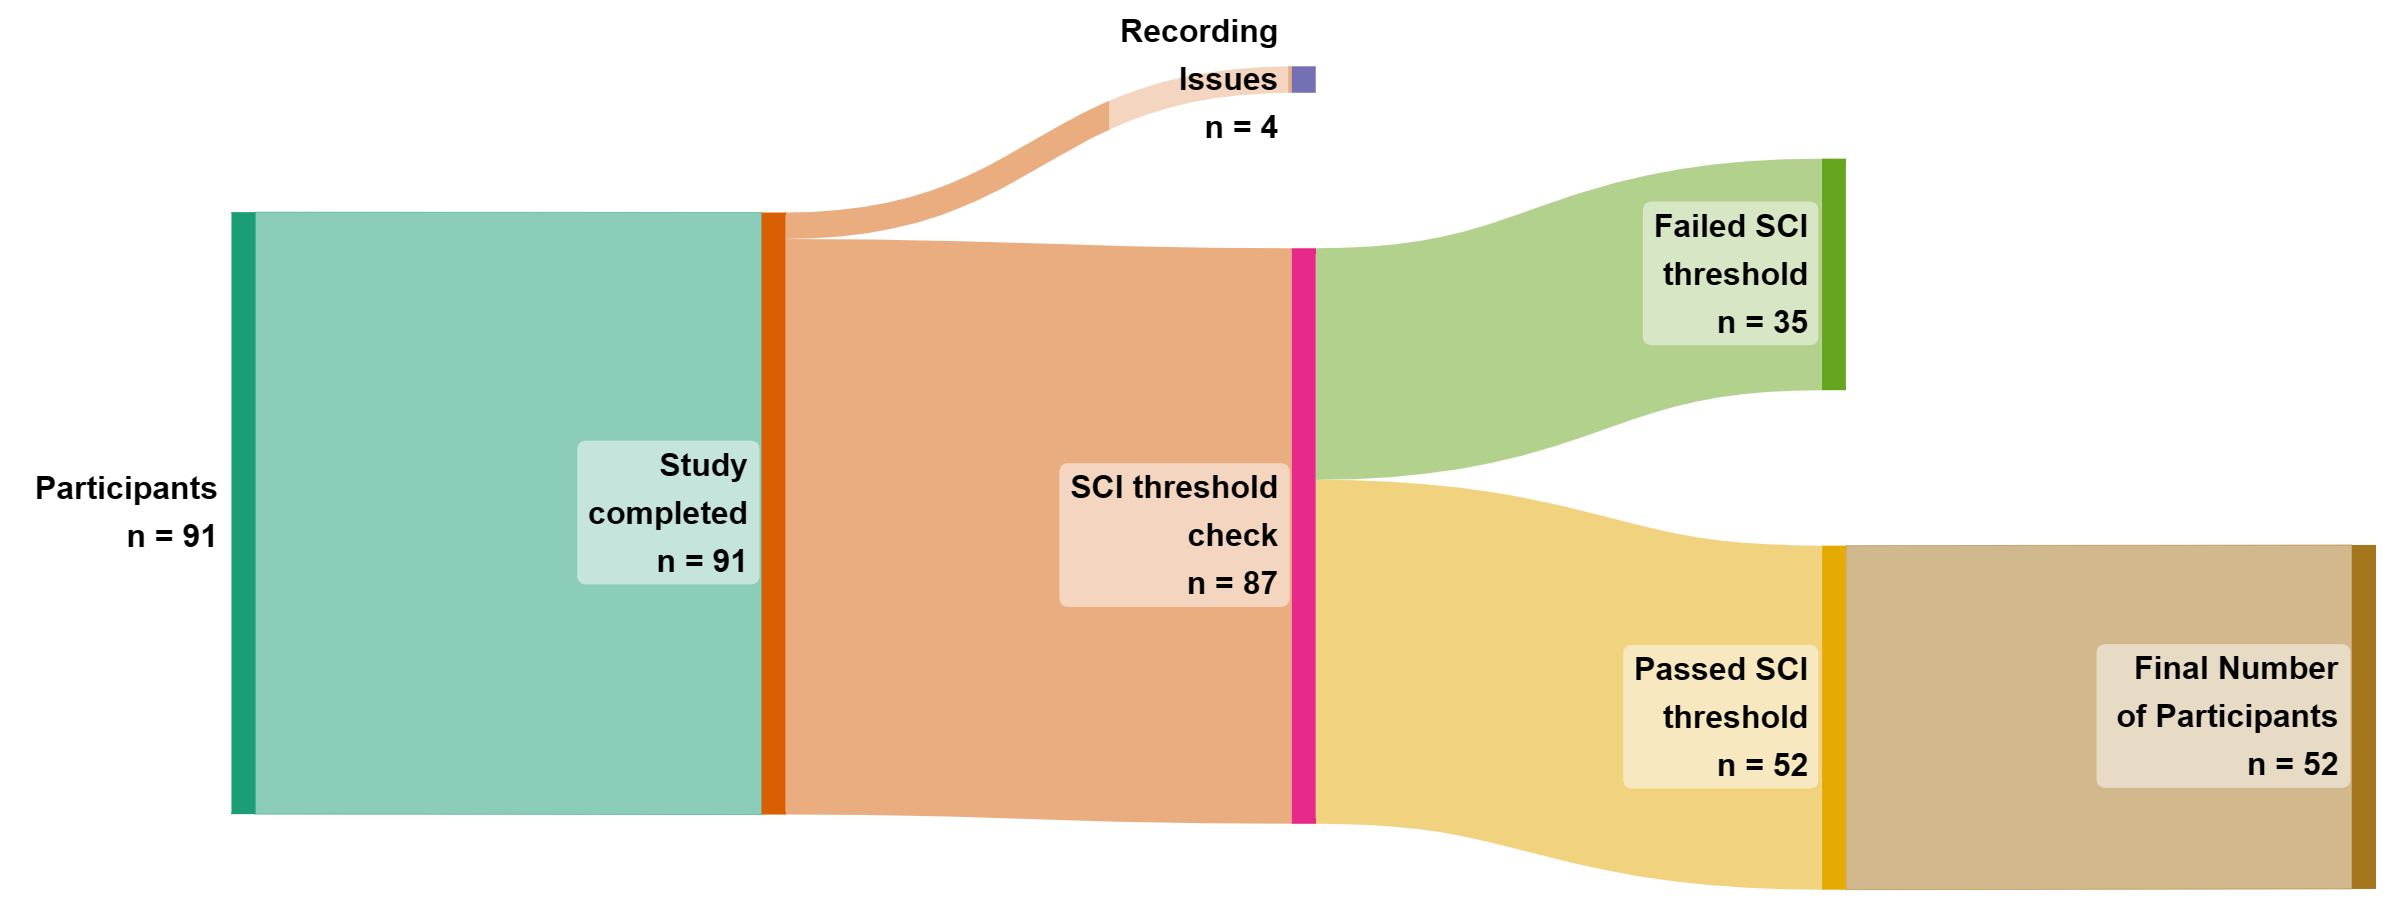
\includegraphics[width=\textwidth]{C:/Users/super/OneDrive - Ontario Tech University/fNIRS_Emotions/plots/figures/Participants Sankey Diagram.png}
        \caption[Participant inclusion flow diagram]{Sankey diagram showing the flow of participants through each stage of inclusion/exclusion in the study.}
        \label{fig:participants_sankey}
    \end{subfigure}
    \vskip\baselineskip
    \begin{subfigure}[b]{0.85\textwidth}
        \centering
        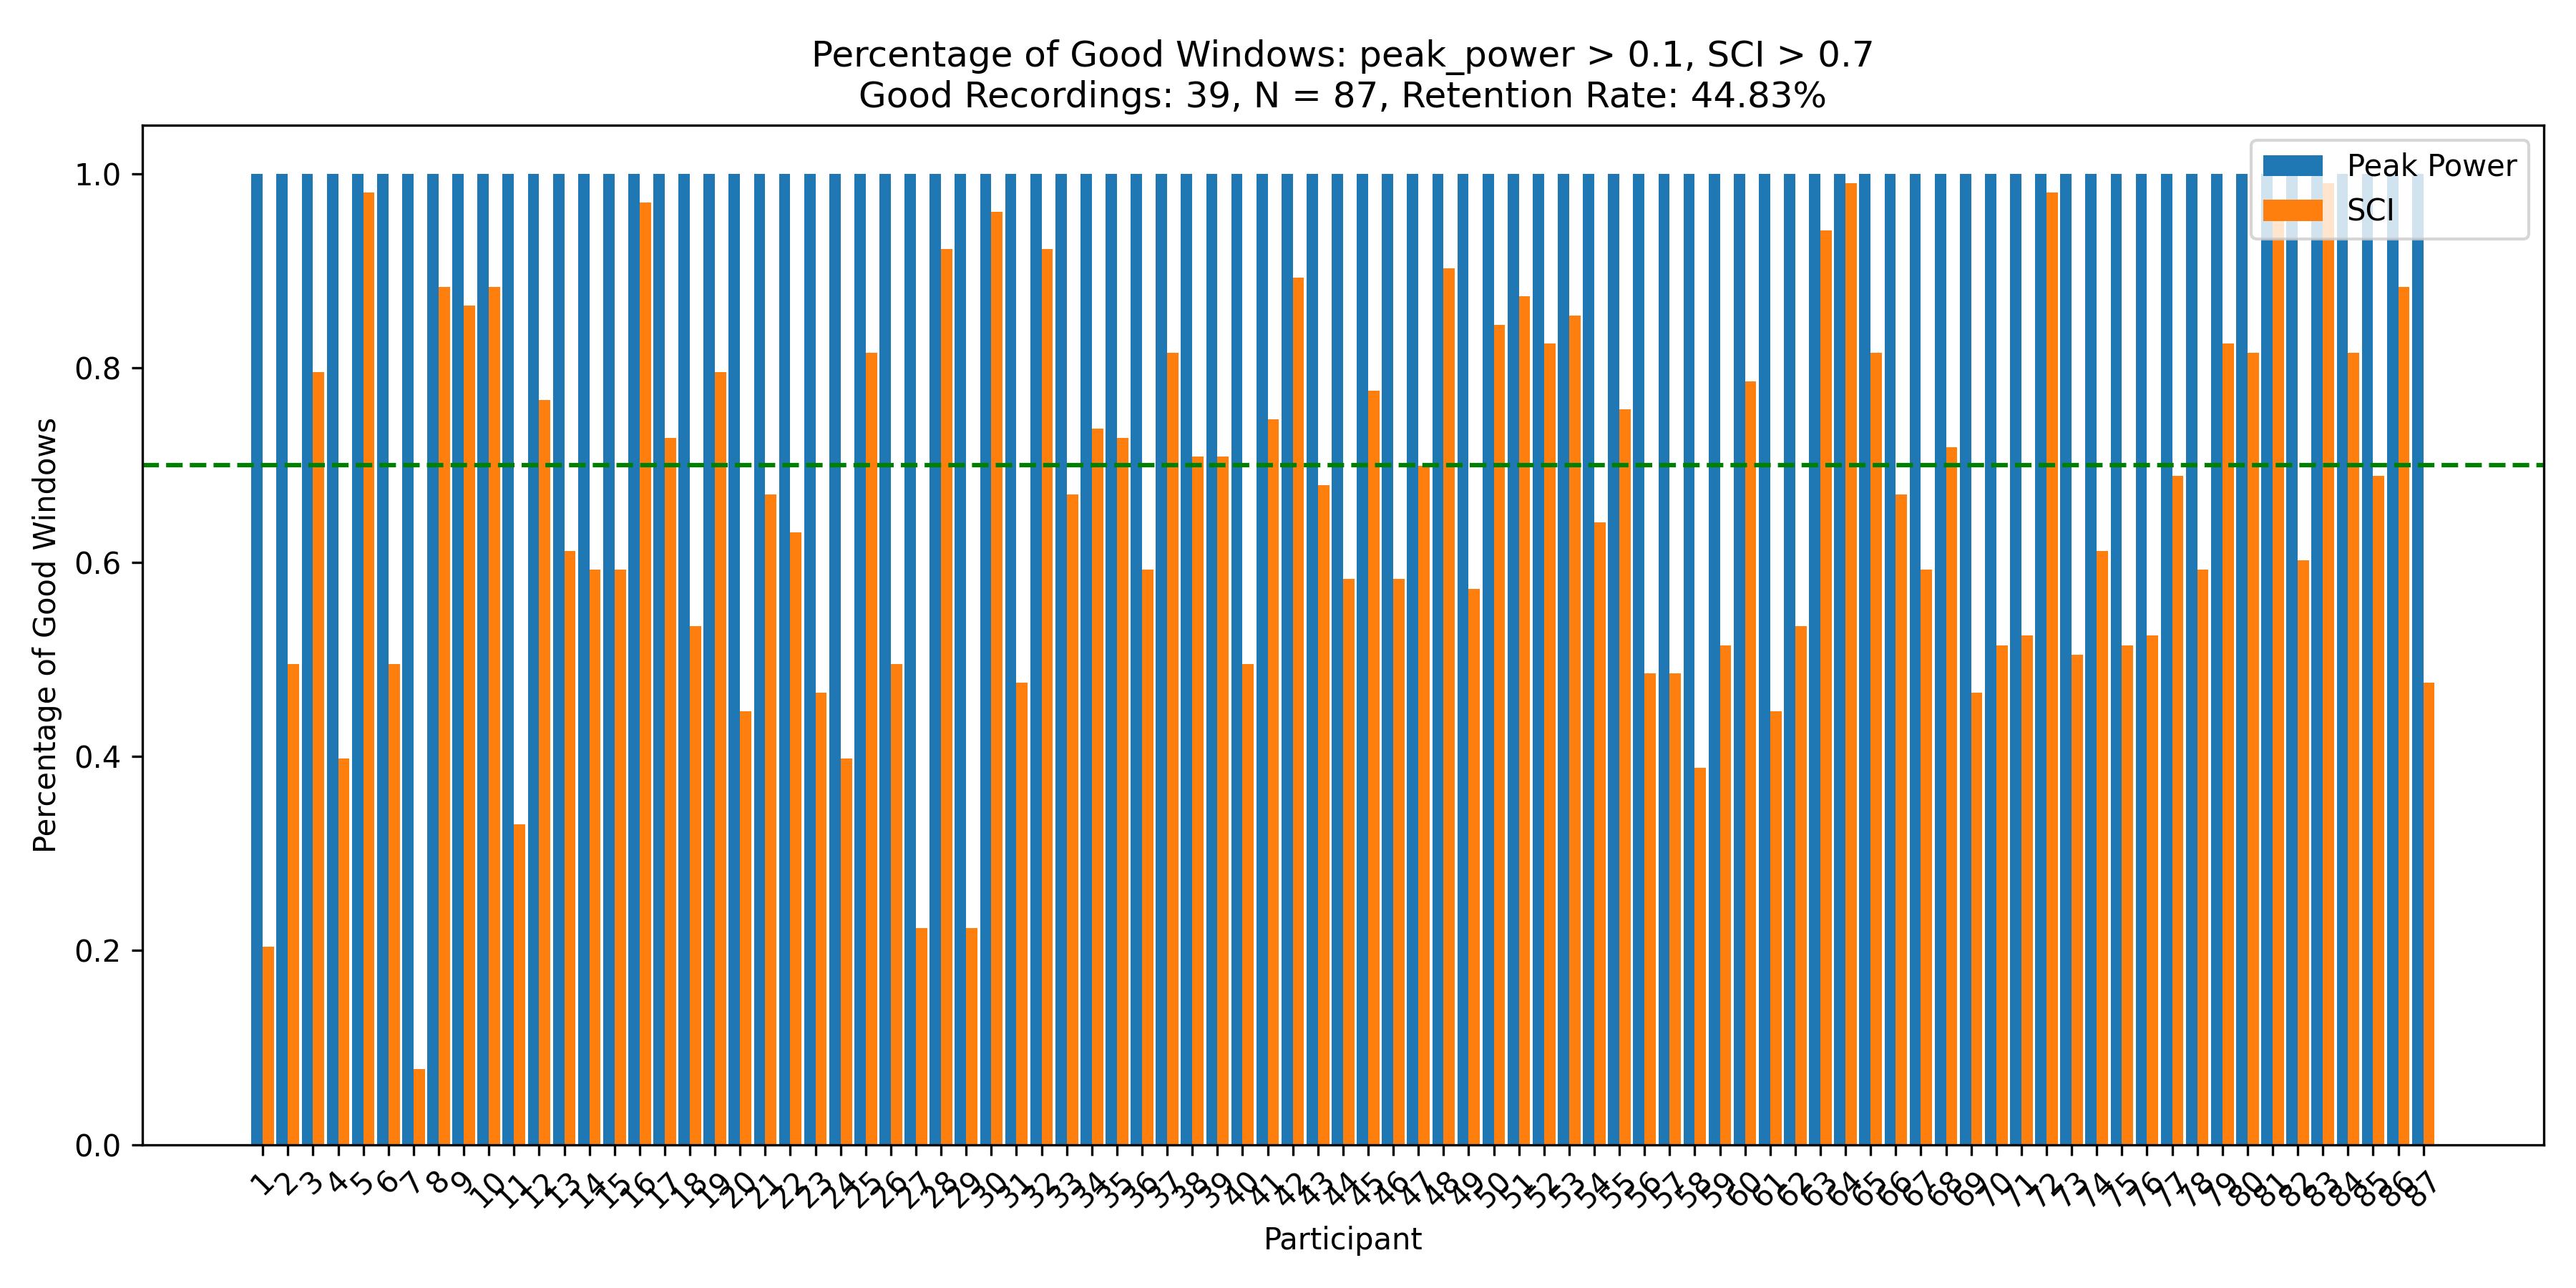
\includegraphics[width=\textwidth]{C:/Users/super/OneDrive - Ontario Tech University/fNIRS_Emotions/plots/signal quality/Percentage of Good Windows.png}
        \caption[SCI signal quality inclusion threshold]{Percentage of Channels where SCI $>$ 0.5 for $>$ 70\% of the windows.
        The green dashed line represents the threshold of 70\% of windows that each participant must meet to be included in the analysis.}
        \label{fig:signal_quality}
    \end{subfigure}
    \caption[Participant signal quality and inclusion flow]{(A) Participant inclusion flow diagram. (B) SCI signal quality inclusion threshold.}
    \label{fig:signal_quality_and_sankey}
\end{figure}

\section{Stimuli and apparatus}
\subsection{Stimuli}
One hundred and forty images of facial expressions from the RADIATE and UIBVFED datasets were used \citep{conley_racially_2018, oliver_uibvfed_2020}.
Then adult models (5 males and 5 females) from each dataset were identified and matched between-sets on face shape, sex, skin tone, and hair colour. 
Images of each model expressing seven emotions (anger, disgust, fear, happiness, sadness, surprise, neutral) were selected. 
Expressions were selected for each model, that closely align with Ekman's 6 basic emotions + neutral \citep{ekman1971constants}.
UIBVFED images were cropped to the same size as RADIATE images. 

\subsection{Apparatus}
Participants were tested individually in a quiet dedicated testing room. 
Stimuli were presented on a Dell U2415 24-inch monitor at 1920x1200 60Hz. 
Participants were seated in a comfortable non-movable chair, with the monitor placed at eye level. 
Stimuli were presented using PsychoPy3 Experiment Builder (v2024.1.5) \citep{peirce_psychopy2_2019}. 
Participant brain activity was recorded using Aurora fNIRS while participants completed the task. 
fNIRS data was collected using two NIRSport2 systems (NIRx Medical Technologies, Berlin, Germany). 
Each NIRSport2 system was equipped with 16 source and 16 detector optodes, and daisy-chained together for a high density 32x32 optode configuration. 
Each neighboring pair of source and detector optode is referred to as a channel, resulting in a total of 103 HbO + 103 HbR channels (plus 16 short distance channels).
The average distance between source and detector optodes was 30 mm, and 7mm for short distance channels, which were placed on a flexible fNIRS head cap (NIRScap) 58 cm in circumference. 
The optodes were arranged in a high density 32x32 montage with one bundle of short distance channels, as shown in Figure \ref{fig:montage_combined}.
This montage was designed to cover a maximally large area of the brain, given increasing evidence that emotion processing is not localized to specific discrete areas of the brain, rather distributed across the brain \citep{lindquist_brain_2012}. 
The fNIRS cap and optodes were positioned following the 10-20 international coordinate system.
Light was emitted at 760 nm and 850 nm wavelengths, and the sampling rate was approximately 6.105 Hz.

\begin{figure}[H]
    \centering
    \begin{subfigure}[b]{1\textwidth}
        \centering
        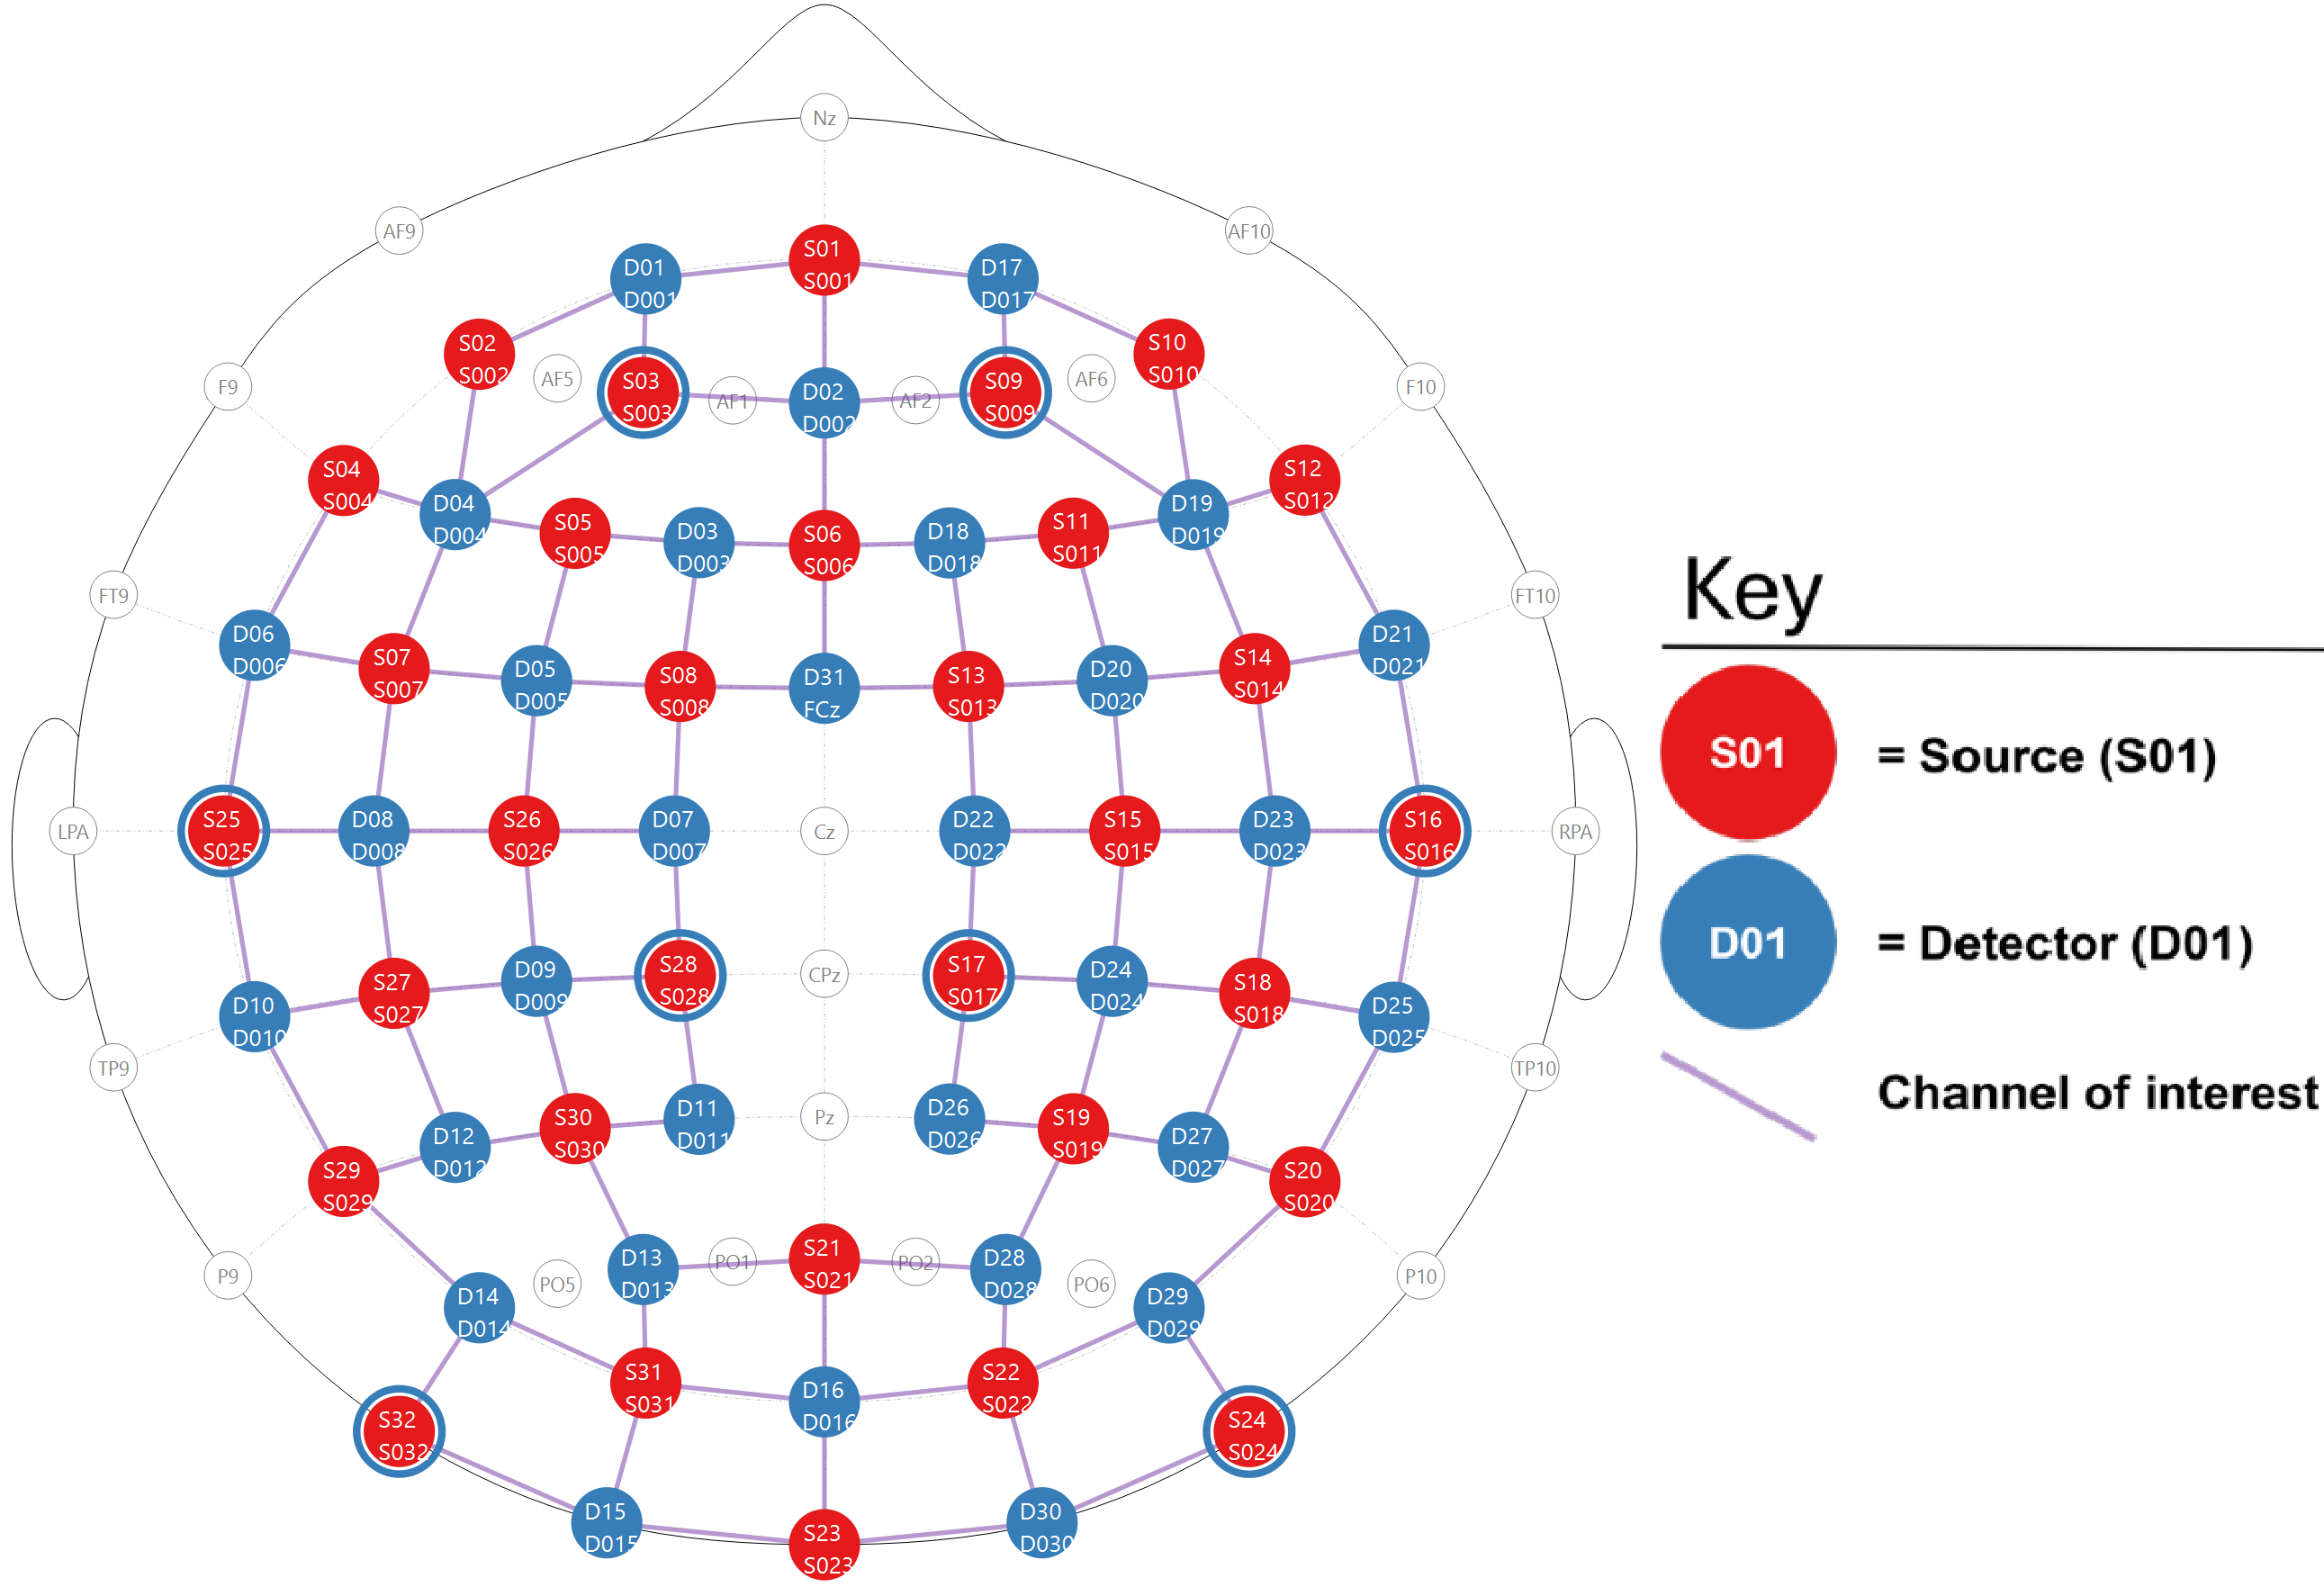
\includegraphics[width=\textwidth]{C:/Users/super/OneDrive - Ontario Tech University/fNIRS_Emotions/plots/figures/Montage.png}
        \caption[Montage depictions]{Depictions of the high density 32x32 optode montage. Red circles represent sources, blue circles represent detectors, the colored lines represent channels, and blue rings around sources represent the locations of the 8 short distance detectors.
        The colors of the channels represent the regions of interest (ROI's) that the channels were grouped into, see (b) for the corresponding brain region labels.}
        \label{fig:montage}
    \end{subfigure}
    \vskip\baselineskip
    \begin{subfigure}[b]{0.45\textwidth}
        \centering
        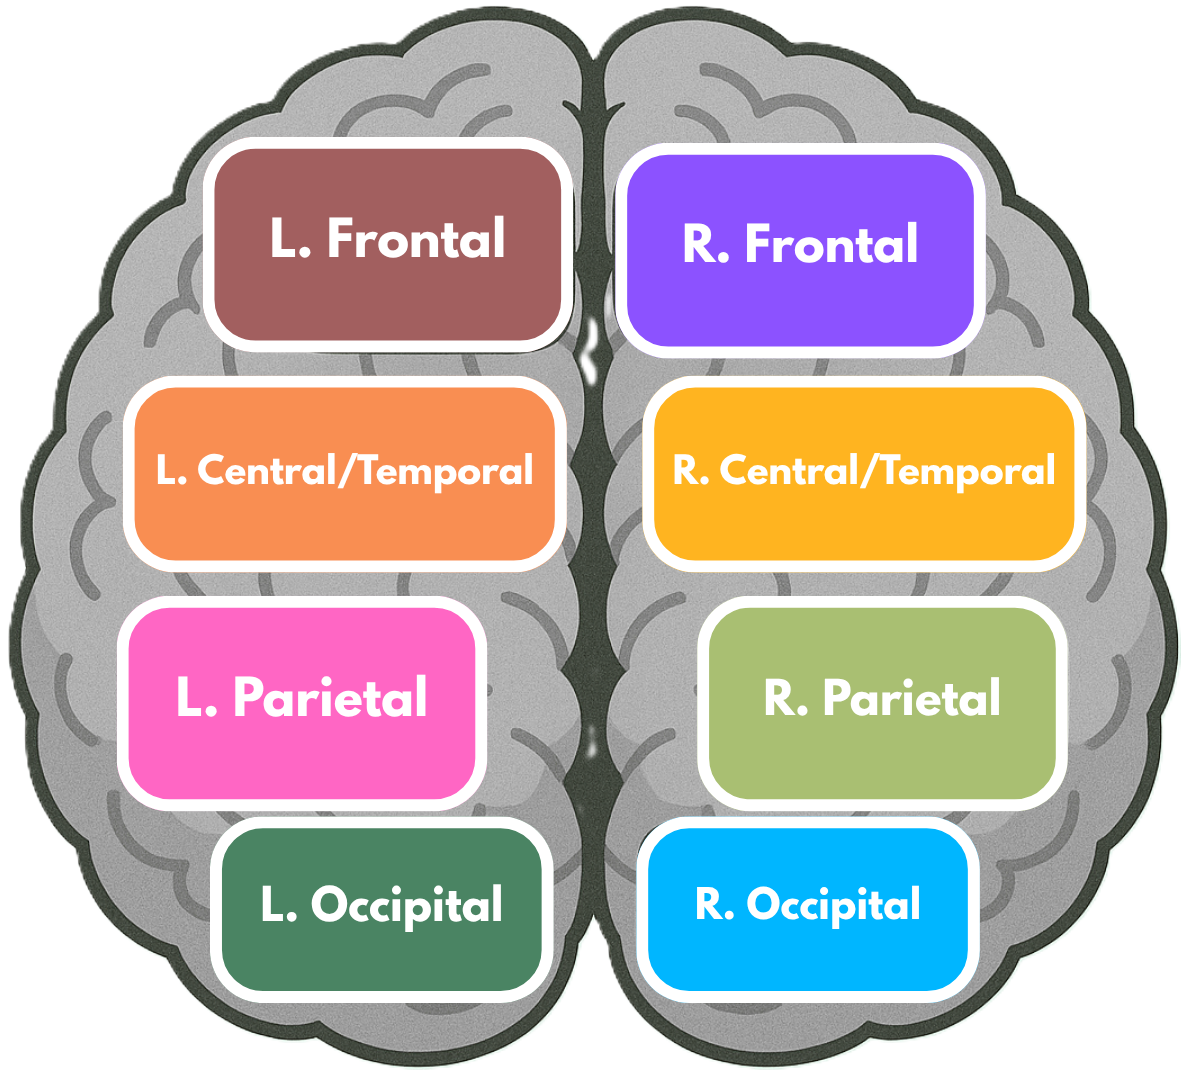
\includegraphics[width=\textwidth]{C:/Users/super/OneDrive - Ontario Tech University/fNIRS_Emotions/plots/figures/Brain Region Map.png}
        \caption[Brain region map for ROI grouping]{Brain region map, showing the regions of interest (ROI's) that the channels were grouped into for certain analyses.}
        \label{fig:brain_region_map}
    \end{subfigure}
    \caption[Montage and brain region map]{(a) High density 32x32 optode montage. (b) Brain region map for ROI grouping.}
    \label{fig:montage_combined}
\end{figure}

\section{Design and procedure}
\subsection{Design}
\label{sec:Design}
A full-factorial Face-type (2 levels: Real, Virtual) \texorpdfstring{$\times$}{x} Emotion (7 levels: Anger, Disgust, Fear, Joy, Sadness, Surprise, Neutral) \texorpdfstring{$\times$}{x} Model (4) \texorpdfstring{$\times$}{x} Sex (2 levels: Male, Female) \texorpdfstring{$\times$}{x} Repetition (4) experimental design was used, with each participant presented with 448 images. 
Stimuli were blocked and counterbalanced by Face-type and Emotion. 
Within each of the 56 Face-type-Emotion Blocks, participants were presented with 8 distinct model faces (4 male, 4 female).

\subsection{Procedure}
\label{sec:Procedure}
Following consent and briefing, participant head size was measured and a size-appropriate fNIRS cap fitted. 
A signal optimization routine was then run within Aurora fNIRS to optimize participant channel signal levels. 
This routine worked by increasing source brightness in a stepwise manner, until the optimal signal levels for all channels was reached. 
Following optimization, participants were told that they would be presented with a series of facial expression images and asked to identify whether a probe face matched one of the faces they saw in the preceding block. 
Room lights were then switched off to avoid interference with the fNIRS cap, and participants were monitored from an adjacent room with a live camera feed. 

The experiment began with instructions presented on screen. 
The trial timeline, shown in Figure \ref{fig:paradigm}, consisted of three main epochs: fixation cross, block presentation, and participant feedback. 
Each Block began with a fixed cross presented for 16 seconds, followed by 8 facial images. 
Facial images were each presented for 1.5 seconds, with a 250-750 ms (M=500 ms) interstimulus interval (ISI) between each face. 
To maintain participant attention, participants completed a memory task after each block. 
In the task, participants were presented with a model image with the same emotional expression as the rest of the block's images, and asked if the model was shown in the preceding block of 8 faces, with feedback provided using the keyboard (y/n). 
The probe face has a 50\% chance of either being in the previous block or not. 
The experiment continued after seven seconds if no feedback was provided. 
Most participants only failed to respond to 1-2 blocks of the 56 blocks, with only a handful of participants failing to respond to up to 5 blocks, as illustrated in Figure \ref{fig:appendix_memory_task_no_response_distribution}.
Participants were given a break every seven blocks, and prompted to enter the space bar when they are ready to continue the experiment. 
After the experiment was completed, the experimenter(s) entered the room, removed the fNIRS cap, and the participant was debriefed about the experiment. 
Participation in the experiment took approximately 35 minutes.

\begin{figure}[H]
    \centering
    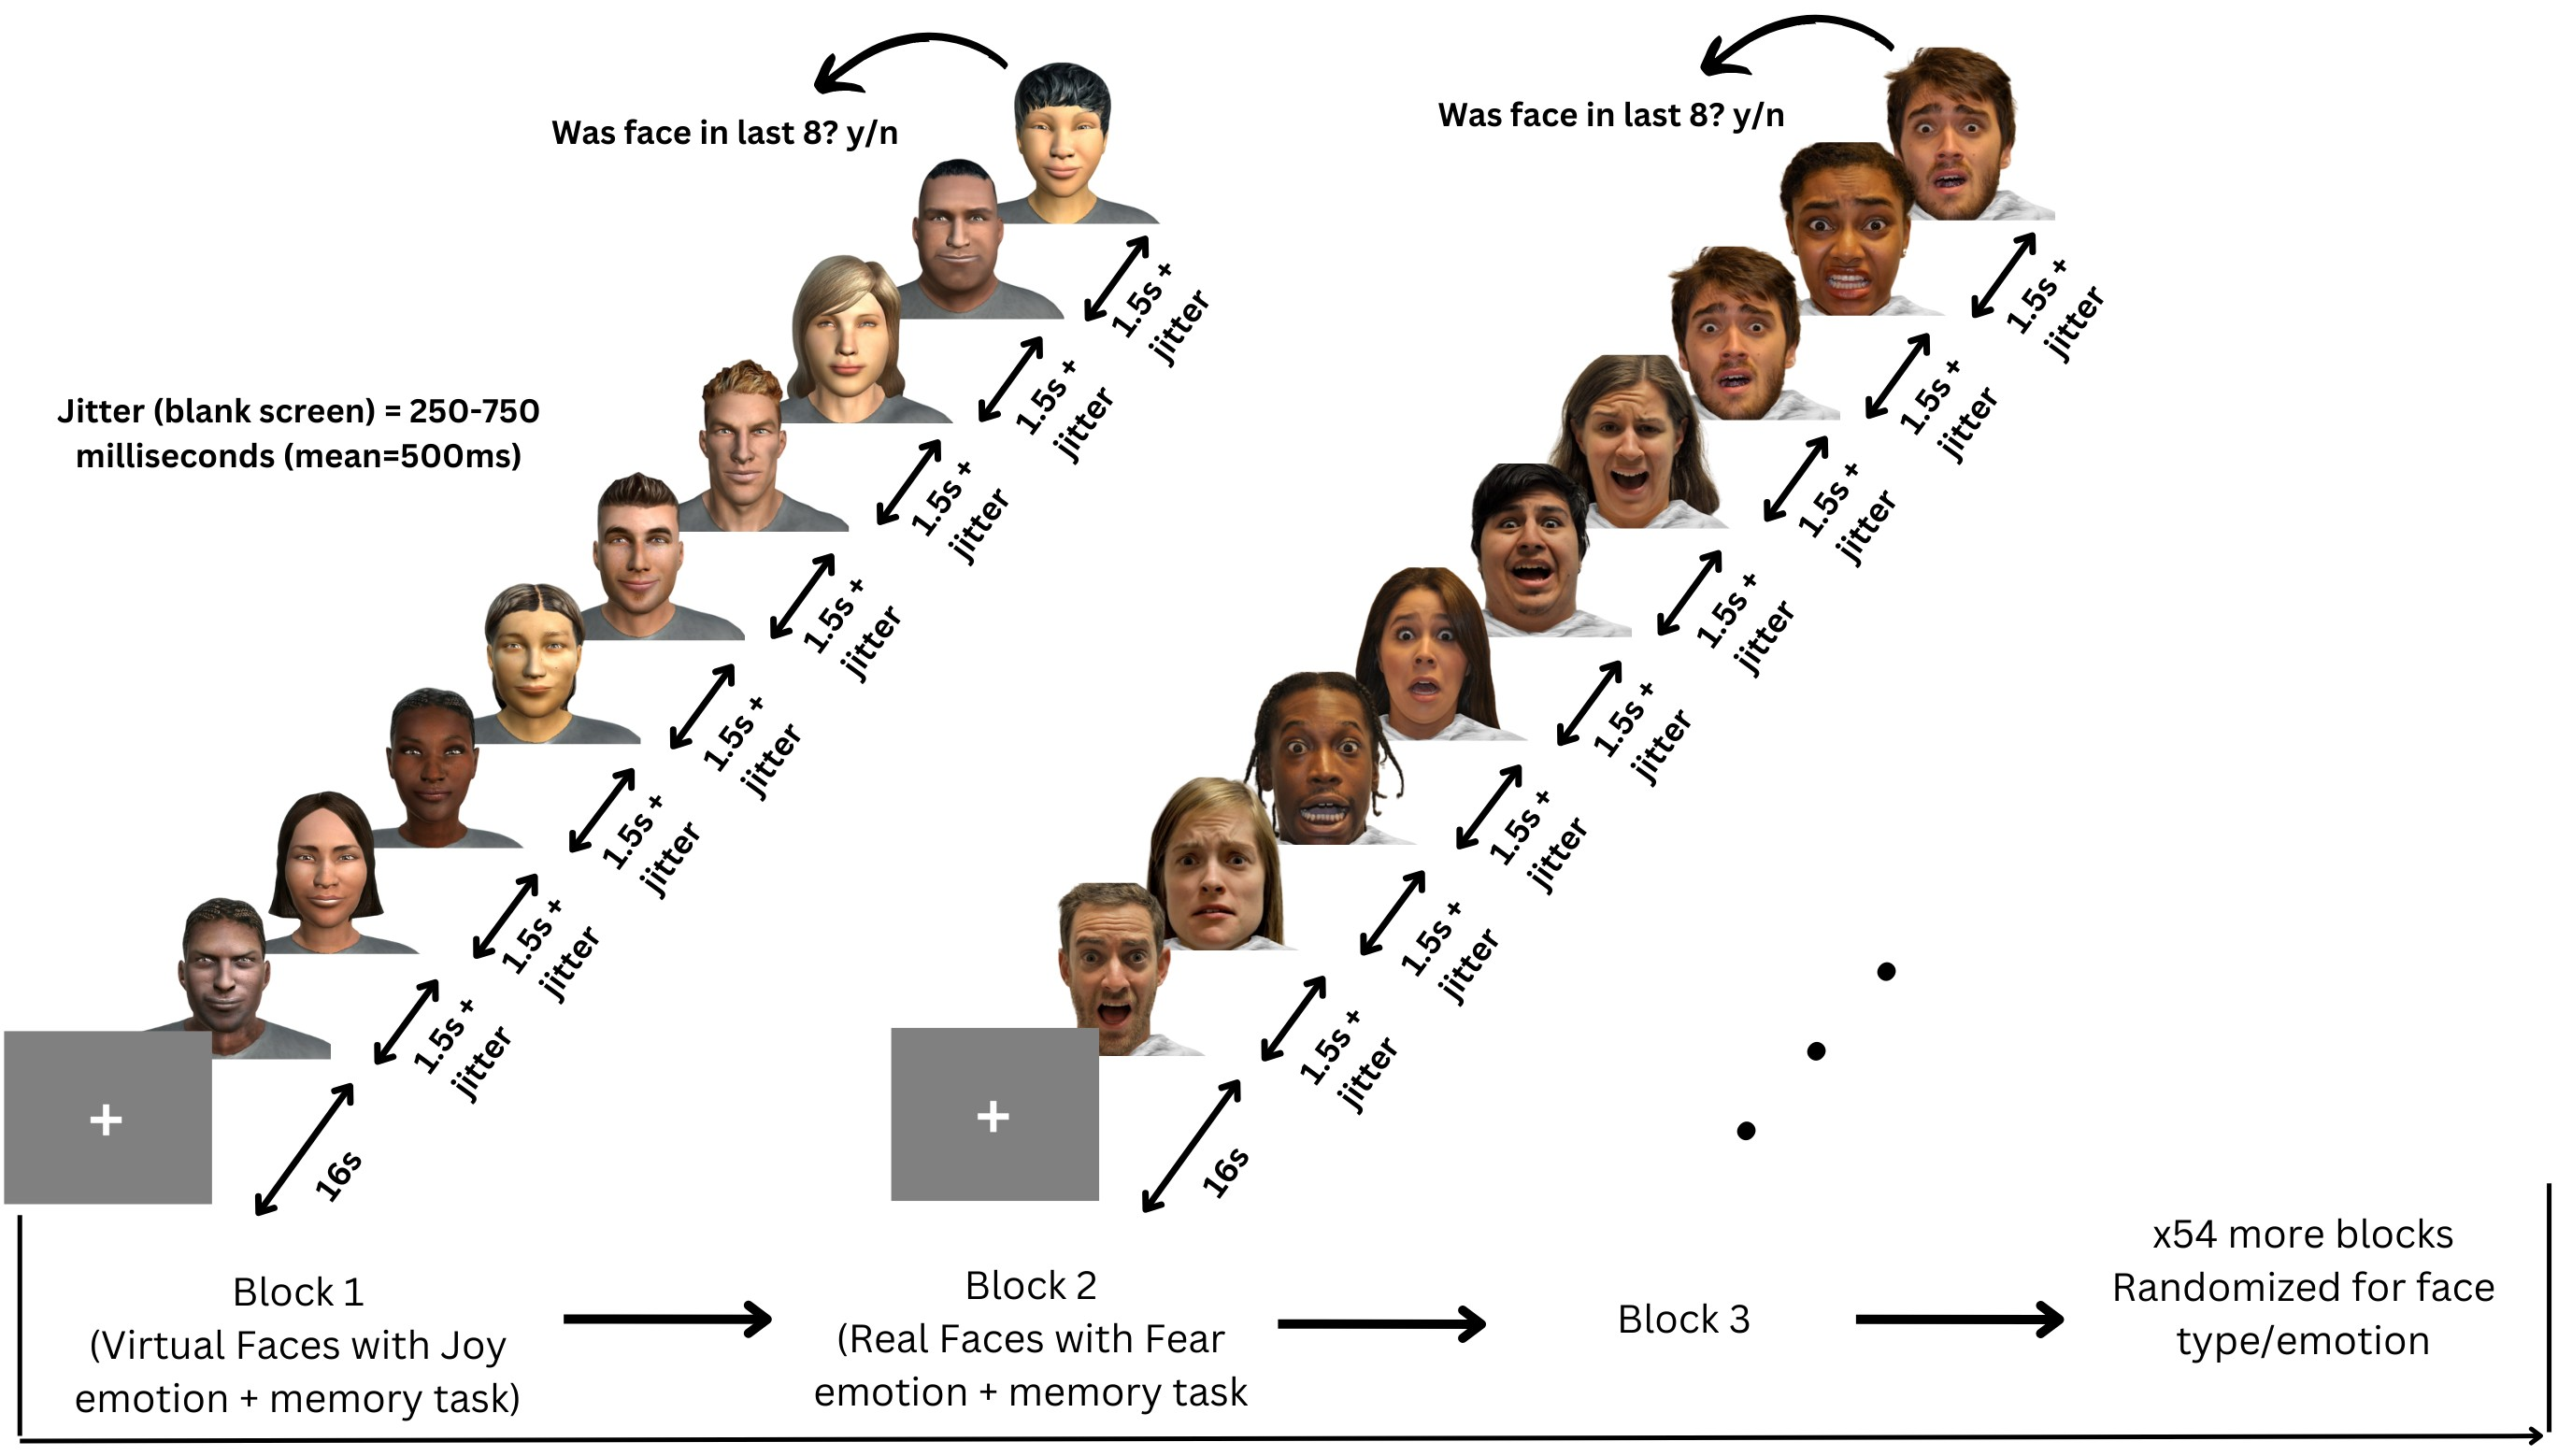
\includegraphics[width=1\textwidth]{C:/Users/super/OneDrive - Ontario Tech University/fNIRS_Emotions/plots/figures/Paradigm.jpg}
    \caption[Experimental paradigm overview]{Participants viewed 56 blocks of 8 faces, each block being either all real or all virtual faces.
    Every face in a block displayed the same emotional expression, one of: anger, disgust, fear, happiness, sadness, surprise, neutral. }
    \label{fig:paradigm}
\end{figure}

\section{Analyses}
All fNIRS data was preprocessed and analyzed with Python 3.11.9 using MNE (version 1.9.0) \citep{gramfort_meg_2013} and MNE-NIRS (version 0.7.1) \citep{luke_analysis_2021}, which used the Nilearn package (version 0.9.2). 
Data were analyzed with a General Linear Model (GLM), followed by a functional connectivity analysis.
The memory task was analyzed in Python using the statsmodels package (version 0.14.4) \citep{seabold2010statsmodels}. 

\subsection{fNIRS preprocessing}
\label{sec:preprocessing}
\begin{figure}[H]
    \centering
    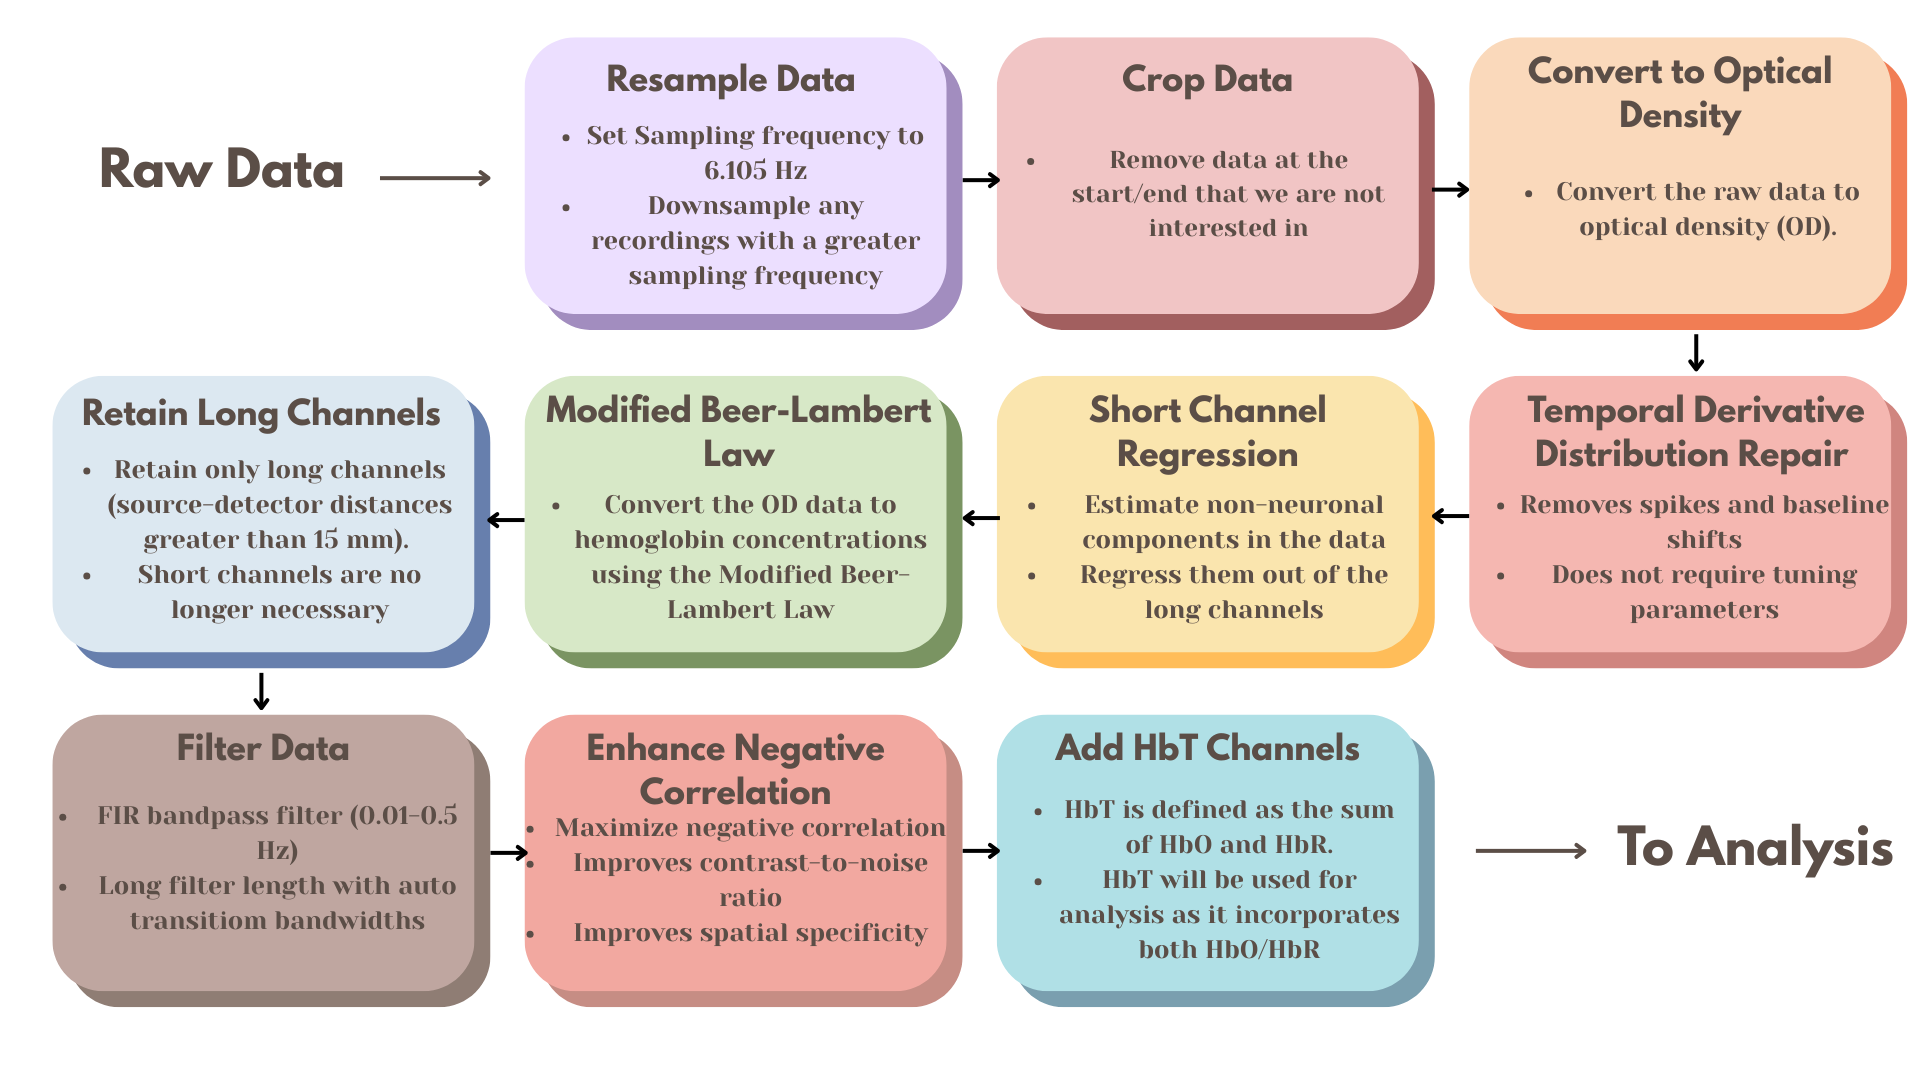
\includegraphics[width=1\textwidth]{C:/Users/super/OneDrive - Ontario Tech University/fNIRS_Emotions/plots/figures/Preprocessing Steps.png}
    \caption[Preprocessing steps for fNIRS data]{Preprocessing steps for fNIRS data, from the raw data to the fully processed data. }
    \label{fig:preprocessing_steps}
\end{figure}

The preprocessing steps for the fNIRS data, as shown in Figure \ref{fig:preprocessing_steps}, were as follows:
1) Downsample the data if the sampling frequency is greater than 6.105 Hz, the initial two datasets were sampled higher than 6.105 Hz, and the sampling frequency should be consistent across all datasets.
2) Crop the data to the first and last annotation. This gets rid of the extra data at the beginning and end of the recording that are not of interest.
3) Convert the raw data to optical density.
4) Apply temporal derivative distribution repair to the OD data \citep{fishburn_temporal_2019}. TDDR is effective at removing spikes and baseline shifts from the data. 
5) Apply short channel regression to the OD data \citep{scholkmann_measuring_2014}. Short channels are used to estimate the superficial hemodynamics (non-evoked/extracerebral/systemic components) in the data, and then regress it out of the long channels \citep{tachtsidis_false_2016}. 
6) Convert the OD data to hemoglobin concentrations using the modified Beer-Lambert law. The MBLL relates the change in light attenuation to the change in hemoglobin concentration of chromophores in the tissue \citep{kocsis_modified_2006}.
7) Retain only long channels (source-detector distance $>$ 15 mm). Since the short channels have already been regressed out, it is no longer necessary to keep them in the data.
8) This FIR bandpass filter extracts signal components in the 0.01-0.5 Hz range, it uses a long filter length (2015 samples) with automatically determined transition bandwidths by MNE-Python \citep{pinti_current_2019}. 
9) Maximizes negative correlation between HbO and HbR \citep{cui_functional_2010}. This method removes spikes, improves contrast-to-noise ratio, and improves spatial specificity of the data.
10) Add HbT (hemoglobin total) channels to the data. HbT is defined as the sum of HbO and HbR. Often, fNIRS studies will only use either one of HbO or HbR channels (more frequently HbO), leaving out one channel with no justification \citep{kinder_systematic_2022}. Therefore, HbT channels are chosen, as HbT makes use of both HbO and HbR channels, and using both hemoglobin species improves the inferences as to where activation occurs \cite{hocke_automated_2018}.

Variable length epochs were created for each block of 8 faces, which were 14-18 seconds long (mean = 16s), depending on the ISI's (see \ref{sec:Procedure}).
Epochs were sorted by Face Type (Real, Virtual), and Emotion (Anger, Disgust, Fear, Happiness, Sadness, Surprise, Neutral), and their interaction.
Baseline correction was applied to remove any constant or slowly varying offsets in the data. 
The data was annotated with the onsets and offsets of each block, along with the duration and condition of each block. 
Block data were then analysed using a GLM and Functional Connectivity analysis. 

\subsection{Activation magnitude with General Linear Model (GLM)}
\label{sec:GLM}
The General Linear Model (GLM) posits that the observed haemodynamic signal at each channel or Region of Interest (ROI) is a linear combination of task-related regressors convolved with a Hemodynamic Response Function (HRF), plus nuisance regressors (e.g., drift) and residual noise. Mathematically, 

\begin{equation}
Y = X\beta + \epsilon,
\end{equation}

where \( Y \) is the observed time series, \( X \) is the design matrix, \( \beta \) represents the parameters to estimate, and \( \epsilon \) denotes the residuals assumed to be Gaussian noise.
Estimation is performed via ordinary least squares (OLS), yielding parameter estimates that quantify condition-specific activation amplitudes.

\subsubsection{Design Matrix}
For each of the epochs, events are defined by their trial type (e.g., emotion or face type), and onsets/offsets relative to the procedure start, and duration.
The design matrix is constructed using Nilearn's \texttt{make\_first\_level\_design\_matrix} by convolving a boxcar function (based on the event timing) with a canonical HRF, which is a model of the expected haemodynamic response to neural activity.
The canonical HRF Statistical Parametric Mapping (SPM) \citep{friston_statistical_2007} is chosen to model neurovascular coupling, this model captures the stereotypical rise and fall of the BOLD/fNIRS response. 
The cosine drift model was utilized, which incorporates discrete cosine transform (DCT) basis functions into the design matrix to model and remove low-frequency drifts.
The selection of the high pass cutoff frequency is guided by the structure of the experimental design. 
The cutoff period is set to twice the duration of the longest inter-trial interval, and each fixation period between epochs (or blocks) is 16 seconds. 
Therefore, a cutoff period of 32 seconds (i.e., \texttt{high\_pass=0.03125} Hz) would be appropriate. 
This ensures that the drift model does not remove task-related signal components that occur at frequencies higher than the cutoff \citep{luke_analysis_2021}.
The design matrix \( X \) and preprocessed time series are fed into MNE's \texttt{run\_glm} function, which computes OLS estimates of \( \beta \) for each channel.

\begin{figure}[H]
    \centering
    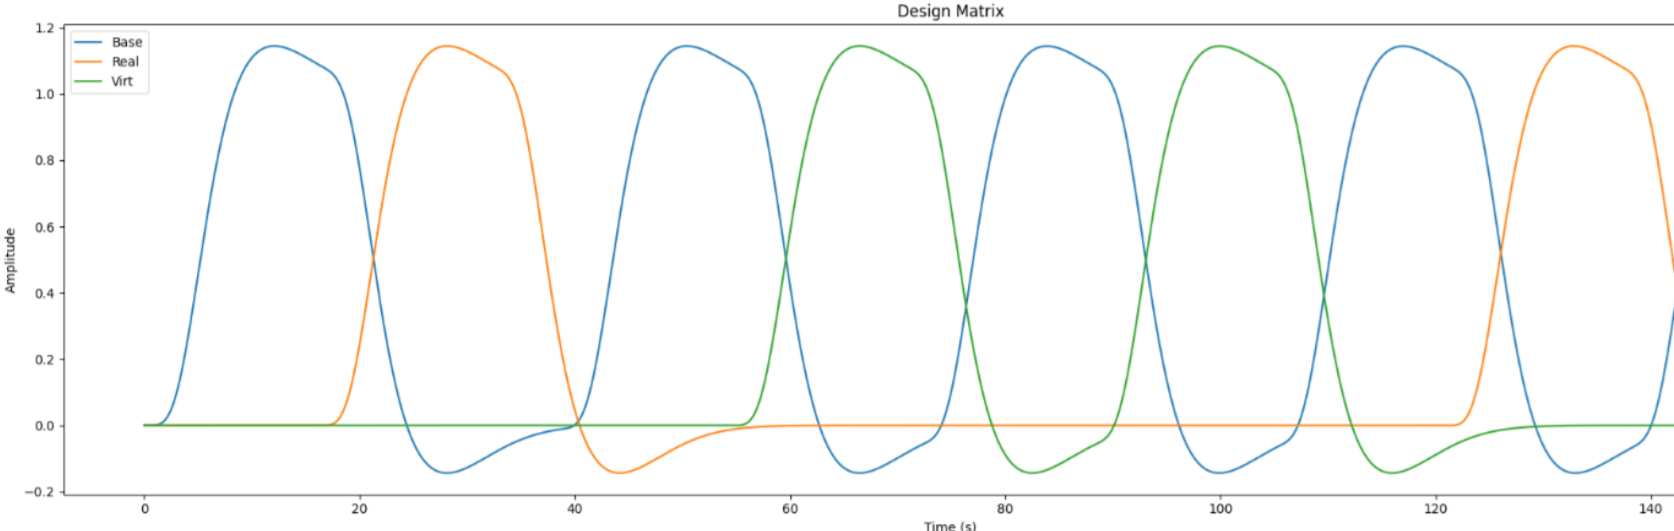
\includegraphics[width=1\textwidth]{C:/Users/super/OneDrive - Ontario Tech University/fNIRS_Emotions/plots/figures/Sample Design Matrix.png}
    \caption[Sample design matrix for GLM]{Sample design matrix for a single participant for the effect Face type, showing the first 7 blocks (250 seconds) of a single experiment.
    The design matrix is organized by condition (Blue for real, orange for virtual), this is the result of convolving the boxcar function with the canonical HRF SPM. }
    \label{fig:design_matrix}
\end{figure}

A two-way repeated measures GLM was conducted on participant's HbT responses by Face-type (2 levels: Real, Virtual) and Emotion (7 levels: Anger, Disgust, Fear, Joy, Sadness, Surprise, Neutral). 
Pairwise contrasts were then computed between conditions to identify effects of interest.

\subsubsection{Contrast Computation}
\label{sec:contrast_computation}
All pairwise contrasts were generated between conditions by constructing an identity contrast matrix over design columns. 
For each pair of conditions \( (A, B) \), the contrast vector is defined as: $c = e_A - e_B$, where \( e_A \) and \( e_B \) are the respective design matrix columns for conditions \( A \) and \( B \). 
Contrasts are computed using MNE's \texttt{compute\_contrast} function, which produces effect estimates and test statistics aggregated across channels.
Since numerous statistical tests are performed across channels and contrasts, $p$-values were FDR-corrected corrected using the Benjamini-Hochberg procedure \citep{singh_exploring_2006} with a family-wise error rate of $\alpha$=0.05.

\subsection{Network mapping with Functional Connectivity Analysis}
\label{sec:fc}
To characterize the temporal coordination between fNIRS channels during face and emotion processing, functional connectivity matrices were computed using a continuous wavelet transform (CWT)-based spectral connectivity approach.
CWT decomposes signals into simultaneous time-frequency representations, providing an optimal framework for fNIRS connectivity analysis by accommodating the non-stationary, physiological nature of hemodynamic signals. 
The morlet wavelet, a gaussian function modulated by a sine wave, was picked as they are suited to capture both slow neural rhythms and faster systemic fluctuations in fNIRS data \citep{reddy_evaluation_2021}. 
Wavelet-based approaches have been widely adopted in the fNIRS literature for connectivity and even artifact correction \citep{bergmann_evaluation_2023, hakim_quantification_2023}
Coherence combines both phase and amplitude information into a single, normalized index, 0 (no coupling) to 1 (perfect coupling), and is a richer description of coupling than phase-only or amplitude-only metrics \citep{bastos_tutorial_2016}.

For each participant, MNE's \texttt{spectral\_connectivity\_time} function was applied to compute time-resolved coherence across pairs of channels, the average of this was taken across epochs to obtain a single channel-by-channel connectivity matrix for each condition.
Each participants' connectivity matrix was then averaged across participants to obtain a group-level connectivity matrix for each condition. 
fNIRS hemodynamics predominantly fluctuate in very low frequencies (0.01-0.5 Hz) \citep{reddy_evaluation_2021}. 
The frequency range was narrowed to five evenly spaced frequences between 0.2-0.5 Hz due to short epoch length, this range still targets systemic and neurogenic oscillations while avoiding high-frequency noise \citep{xu_functional_2017}.
Averaging across these closely spaced frequencies reduces data dimensionality, simplifying downstream statistical analyses without sacrificing sensitivity to coupling dynamics. 

\subsubsection{Paired Sample t-tests}
For each mode (Face type/Emotion), and pair of conditions (e.g., Joy vs. Fear), individual-level connectivity matrices were extracted by averaging across epochs to obtain symmetric channel-by-channel coherence matrices. 
Because coherence values are bounded between 0 and 1 and exhibit skewed distributions \citep{miranda_de_sa_coherence_2009}, Fisher's r-to-z transform (\texttt{atanh}) was applied to each matrix element to normalize the data prior to parametric testing. 
Paired $t$-tests for each unique channel pair ($i > j$) were then conducted across participants using SciPy's \texttt{ttest\_rel}.
This directly tests whether mean connectivity differs between conditions, leveraging the paired design to increase statistical sensitivity \citep{hu_characterizing_2023}. 
Given the large number of channel-pair tests, and similar to the GLM analysis above in \ref{sec:contrast_computation}, $p$-values were FDR-corrected using the Benjamini-Hochberg procedure \citep{singh_exploring_2006} with a family-wise error rate of $\alpha$=0.05.

\subsubsection{ROI Chord Plots}
To distill high-dimensional channel-by-channel connectivity into interpretable inter-regional summaries, we mapped individual fNIRS channels onto anatomically defined ROI's. 
This includes left and right frontal, central/temporal, parietal, occipital regions of the brain as shown in Figure \ref{fig:brain_region_map}, and the channels were grouped into these regions based on their location in the montage.
Since multiple channels may map to the same pair of regions (e.g., several left central/temporal channels connecting to several right occipital channels), we calculated the sum of all signicant channel-pair connections for each ROI pair (separately for positive and negative $t$-values). 
We then subtracted the negative sum from the positive sum, resulting in a single integer representing the net connectivity which was positive if the positive connections outweigh the negative ones, and vice versa.
We then took the top 15\% percentile of each net connectivity value, and set the rest to zero, to show only the strongest connections between regions.
The lines were then plotted using a chord diagram, with the line color indicating the direction of the net connectivity (positive or negative), and the line width indicating the magnitude of the net connectivity (the absolute value of the net connectivity).

\subsubsection{Emotion Summary Ratio Plot}
To summarize the net connectivity between regions for each emotion, we calculated a ratio of positive to negative connections for each emotion pair.
The ratio was calculated by taking the difference of the count of significant channels where the $t$-value was positive and the count of significant channels where the $t$-value was negative, and dividing it by the total number of significant channels for that emotion pair. 
This ratio provides a measure of the net connectivity across all ROI's for each emotion, with a positive ratio indicating that one emotion has a stronger net connectivity than the other, and a negative ratio indicating that the other emotion has a stronger net connectivity.

\subsubsection{Region Summary Plot}
To summarize the net connectivity across all emotions for each region, we summed the number of significantly different channel pairs between each region pair across all emotions, disregarding the direction of the $t$-value.
This provides a measure of the net connectivity across all emotions for each region, showing which regions are more connected across all emotions.
The 3 regions with the highest and lowest number of significant channel pairs are marked, to emphasize the most/least connected regions across all emotions.

\subsection{Memory Task Analysis}
\label{sec:memory_task_analysis}
Raw behavioral data captured from PsychoPy were preprocessed to identify participant keyboard responses. 
The total correct trials per participant were summed. 
Since each block of faces was either all real or all virtual, and all had the same emotional expression (as discussed in \ref{sec:Procedure}), each y/n response was labeled with Face type and Emotion.
An OLS model was fit with accuracy (converted to numeric 0/1) as the dependent variable and categorical predictors for Face Type, Emotion, and their interaction. 
The goal is to determine the main effects of these two factors individually, as well as their interaction, on response accuracy.
A two-way Type III ANOVA (via \texttt{sm.stats.anova\_lm(model, typ=3)}) provided $F$-statistics and $p$-values for main effects and interaction.
This version of the ANOVA is especially suitable when interactions are included in the model, as it calculates each effect after accounting for all other terms.

\chapter{Results}
\section{General Linear Model (GLM) Results}
\subsection{Face Type Contrasts}
\begin{figure}[H]
    \centering
      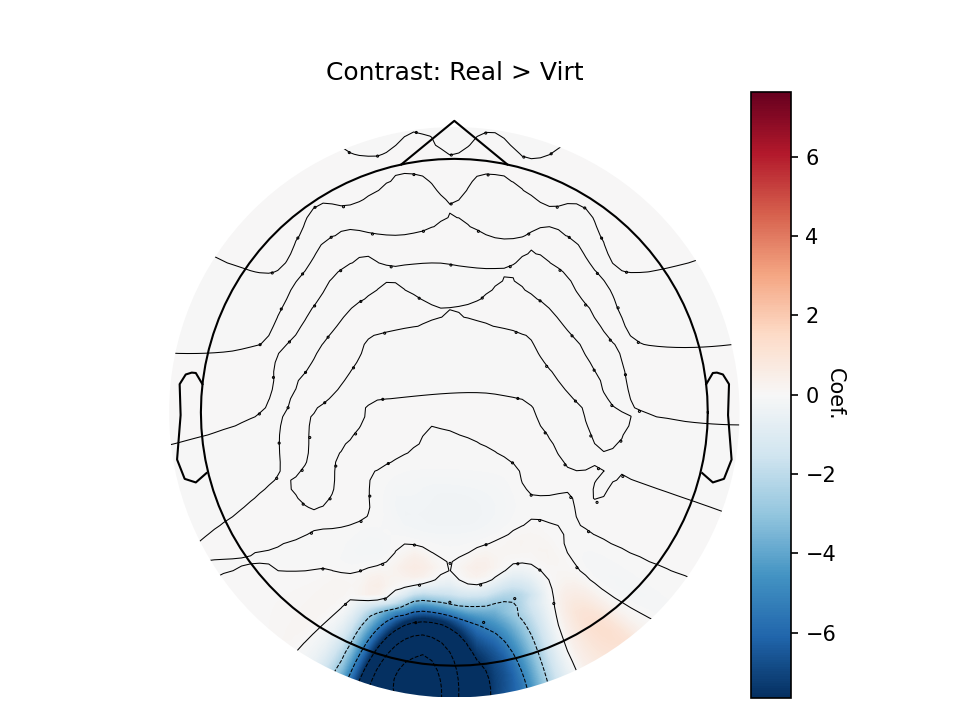
\includegraphics[width=0.85\textwidth]{C:/Users/super/OneDrive - Ontario Tech University/fNIRS_Emotions/plots/glm/contrasts/differences/Contrast_Real-Virt.png}
      \caption[GLM: Real vs. Virtual Faces]{GLM contrast between real and virtual conditions which shows the differences in activation between the two conditions.
      Red signifies that condition 1 (real faces) has more activation in that area than condition 2 (virtual faces), while blue signifies that condition 2 (virtual faces) has more activation than condition 1 (real faces).
      The color bar on the right shows the coefficient of the contrast, which indicates the strength of the difference in activation between the two conditions.}
      \label{fig:glm_real_vs_virtual}
\end{figure}

The main effect of real versus virtual faces (as shown in \ref{fig:glm_real_vs_virtual}) for the GLM revealed a significant difference in activation between real and virtual faces, with the left occipital channel showing greater activation for virtual faces compared to real faces.

\subsection{Emotion Contrasts}
\begin{figure}[H]
    \centering
    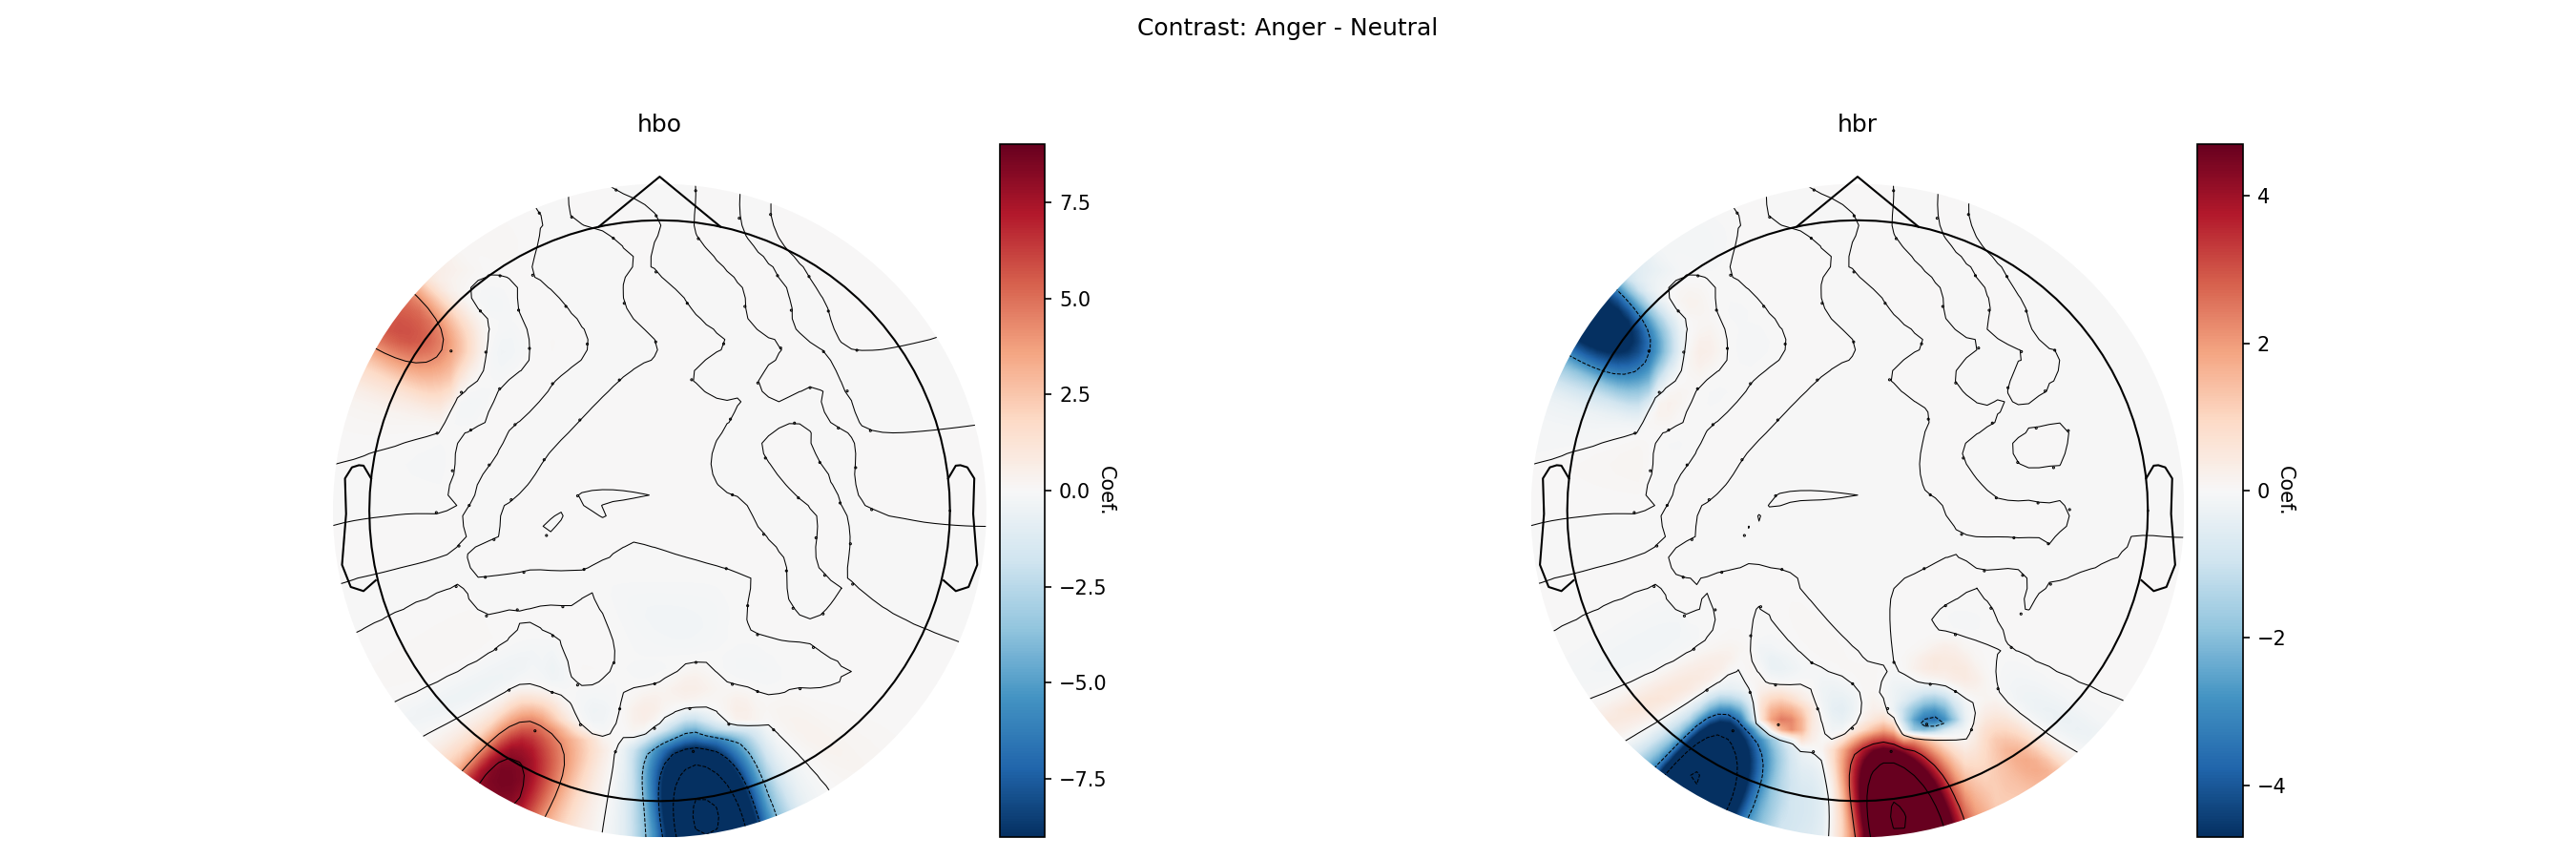
\includegraphics[width=0.45\textwidth]{C:/Users/super/OneDrive - Ontario Tech University/fNIRS_Emotions/plots/glm/contrasts/differences_neutral/Contrast_Anger-Neutral.png}
    
\includegraphics[width=0.45\textwidth]{C:/Users/super/OneDrive - Ontario Tech University/fNIRS_Emotions/plots/glm/contrasts/differences_neutral/Contrast_Fear-Neutral.png}
    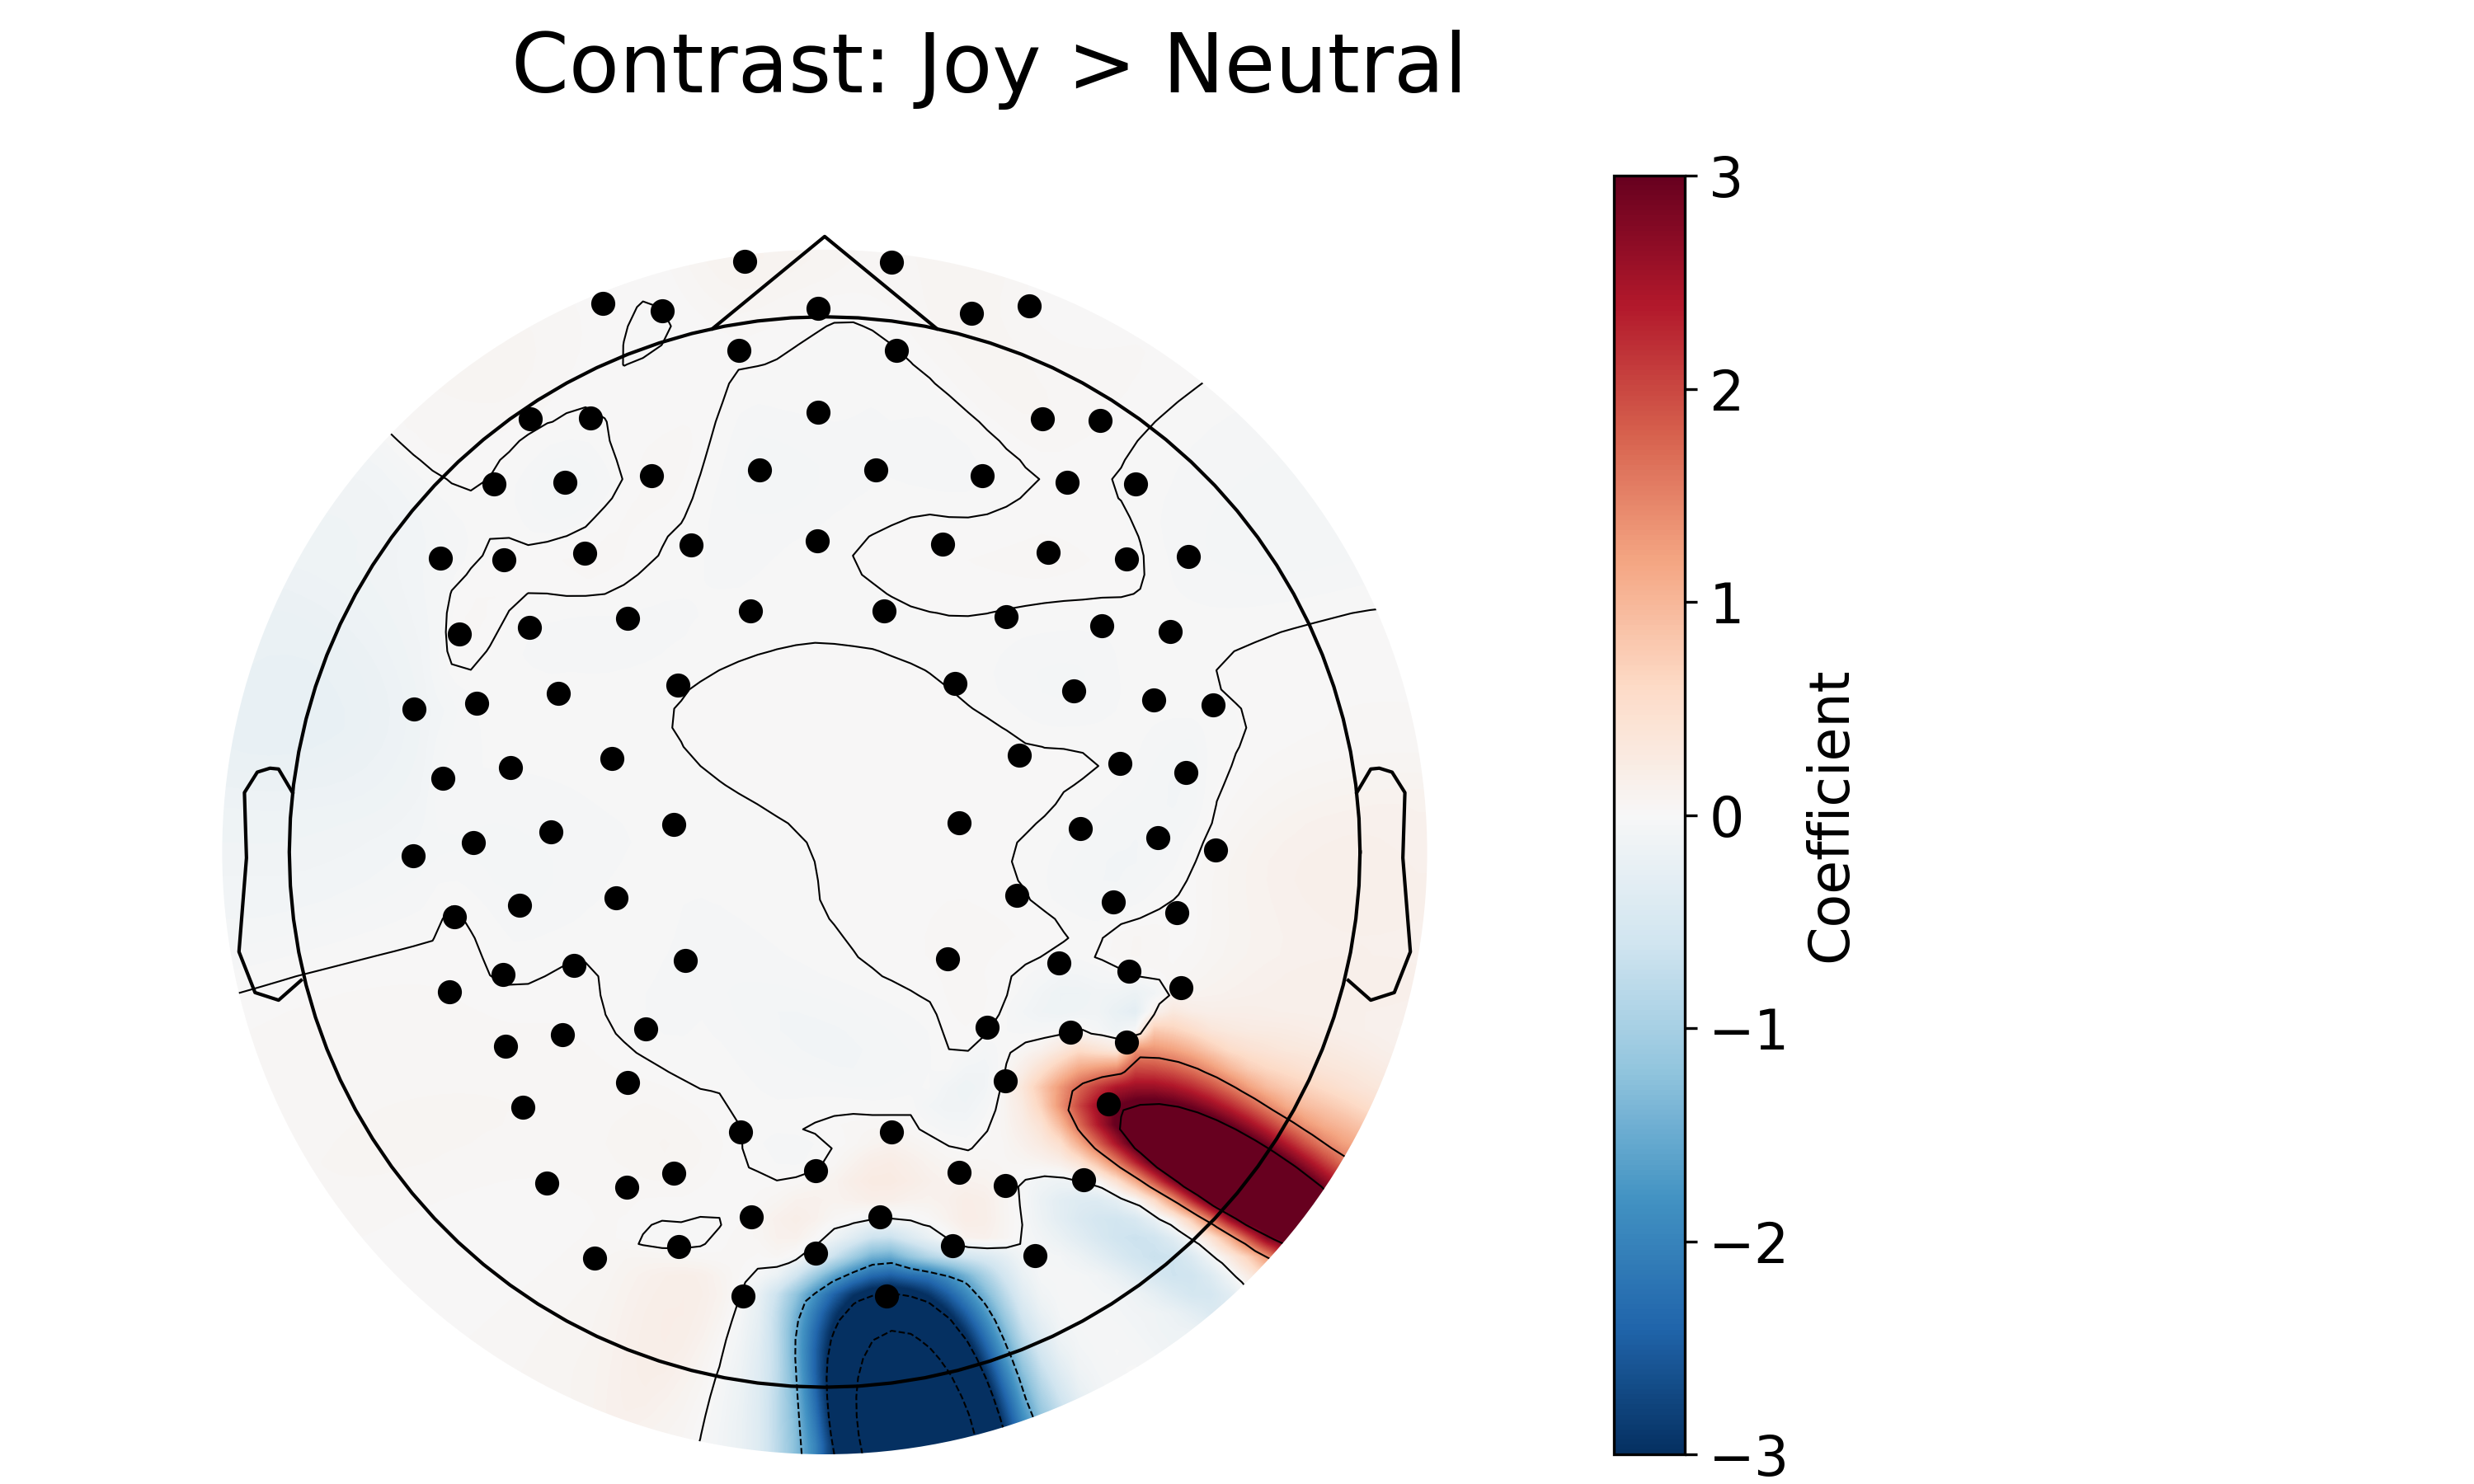
\includegraphics[width=0.45\textwidth]{C:/Users/super/OneDrive - Ontario Tech University/fNIRS_Emotions/plots/glm/contrasts/differences_neutral/Contrast_Joy-Neutral.png}
    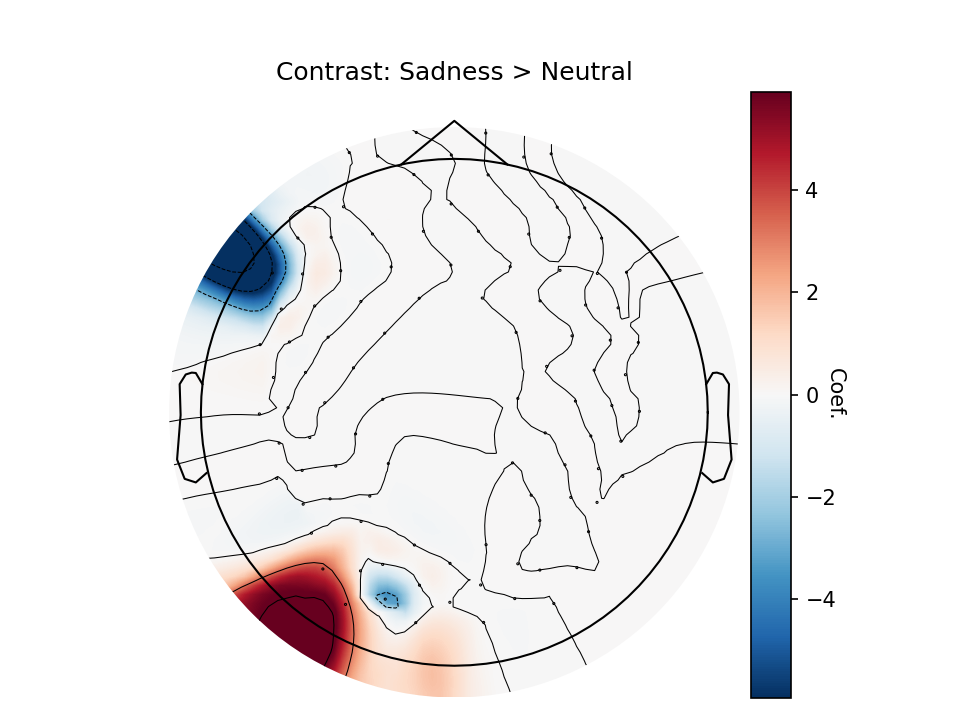
\includegraphics[width=0.45\textwidth]{C:/Users/super/OneDrive - Ontario Tech University/fNIRS_Emotions/plots/glm/contrasts/differences_neutral/Contrast_Sadness-Neutral.png}
    \caption[GLM: Emotion vs. Neutral]{GLM results for the contrast between different emotions and neutral condition.
    Same concept as explained in figure \ref{fig:glm_real_vs_virtual}. }
    \label{fig:glm_emotion_analysis_neutral}
\end{figure}

Against the Neutral emotion (as shown in \ref{fig:glm_emotion_analysis_neutral}), the emotion contrasts revealed significant differences in activation across several brain regions. 
Specifically, Anger and Fear elicited greater activation in the right occipital region compared to Neutral. 
Joy was associated with increased activation in the right parietal region and decreased activation in the right occipital region, while sadness showed reduced activation in the left frontal region relative to Neutral. 
These results indicate distinct neural activation patterns for each emotion when contrasted with the Neutral baseline.

\begin{figure}[H]
    \centering
      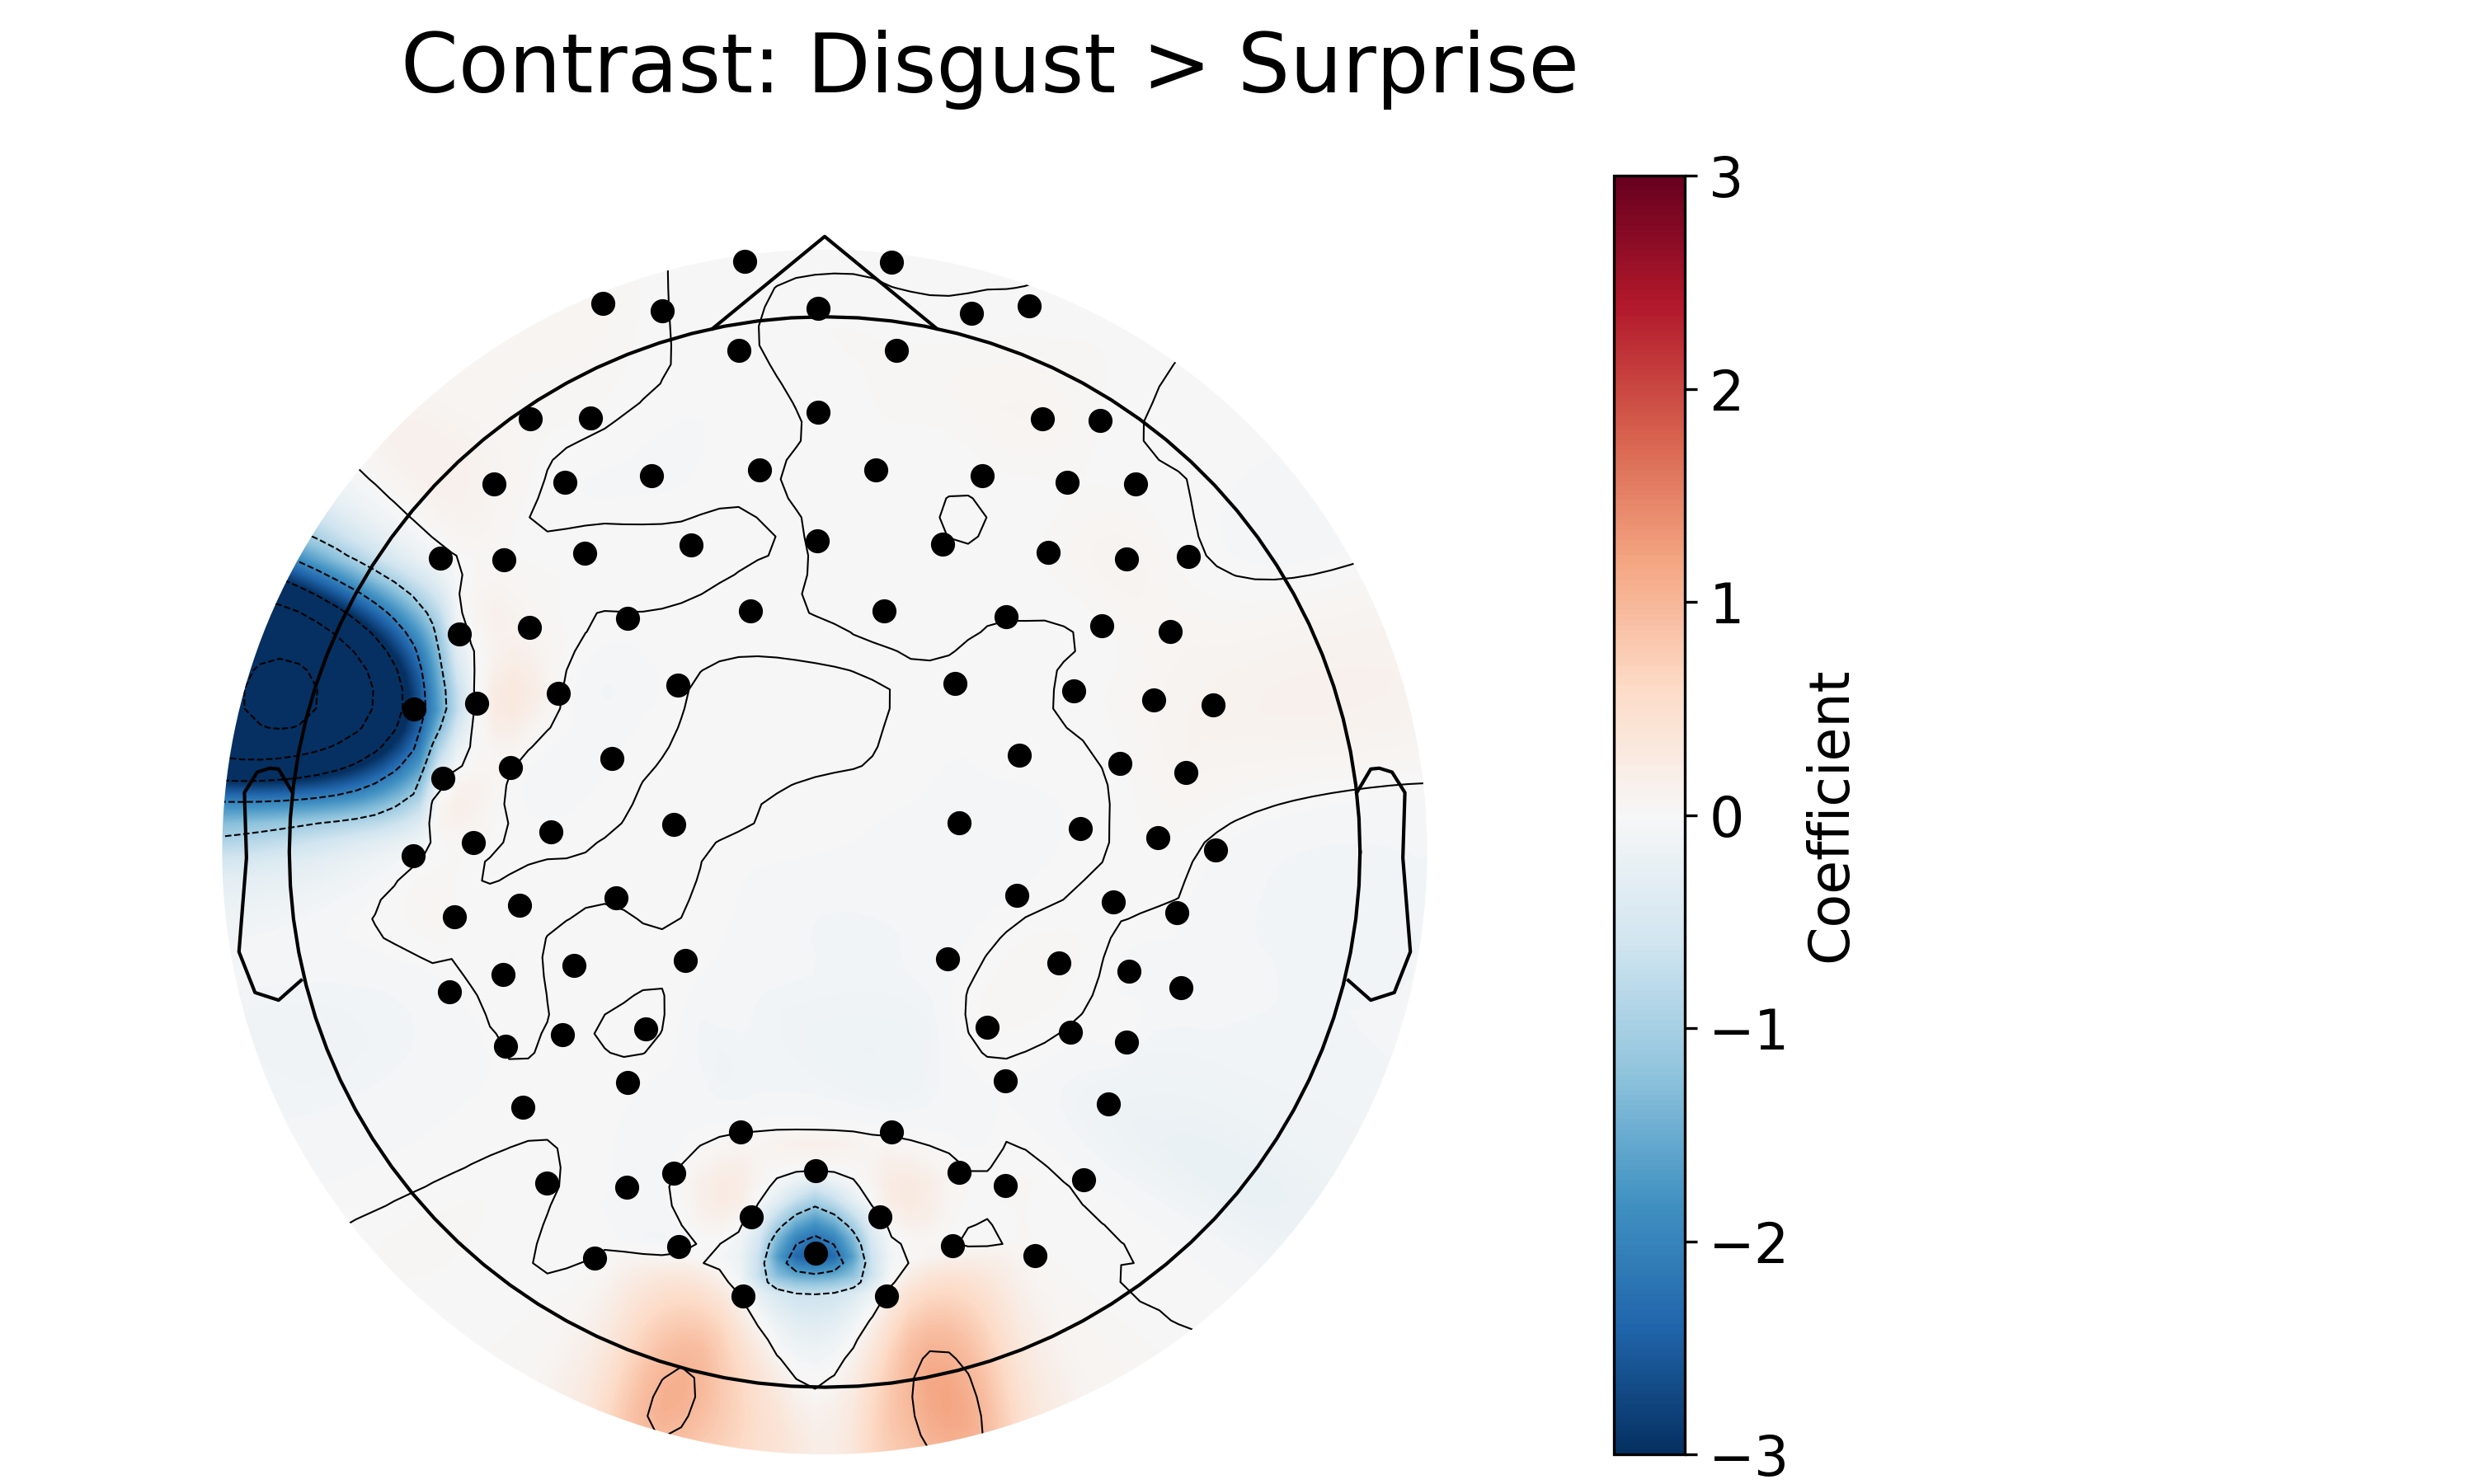
\includegraphics[width=0.45\textwidth]{C:/Users/super/OneDrive - Ontario Tech University/fNIRS_Emotions/plots/glm/contrasts/differences/Contrast_Disgust-Surprise.png}
      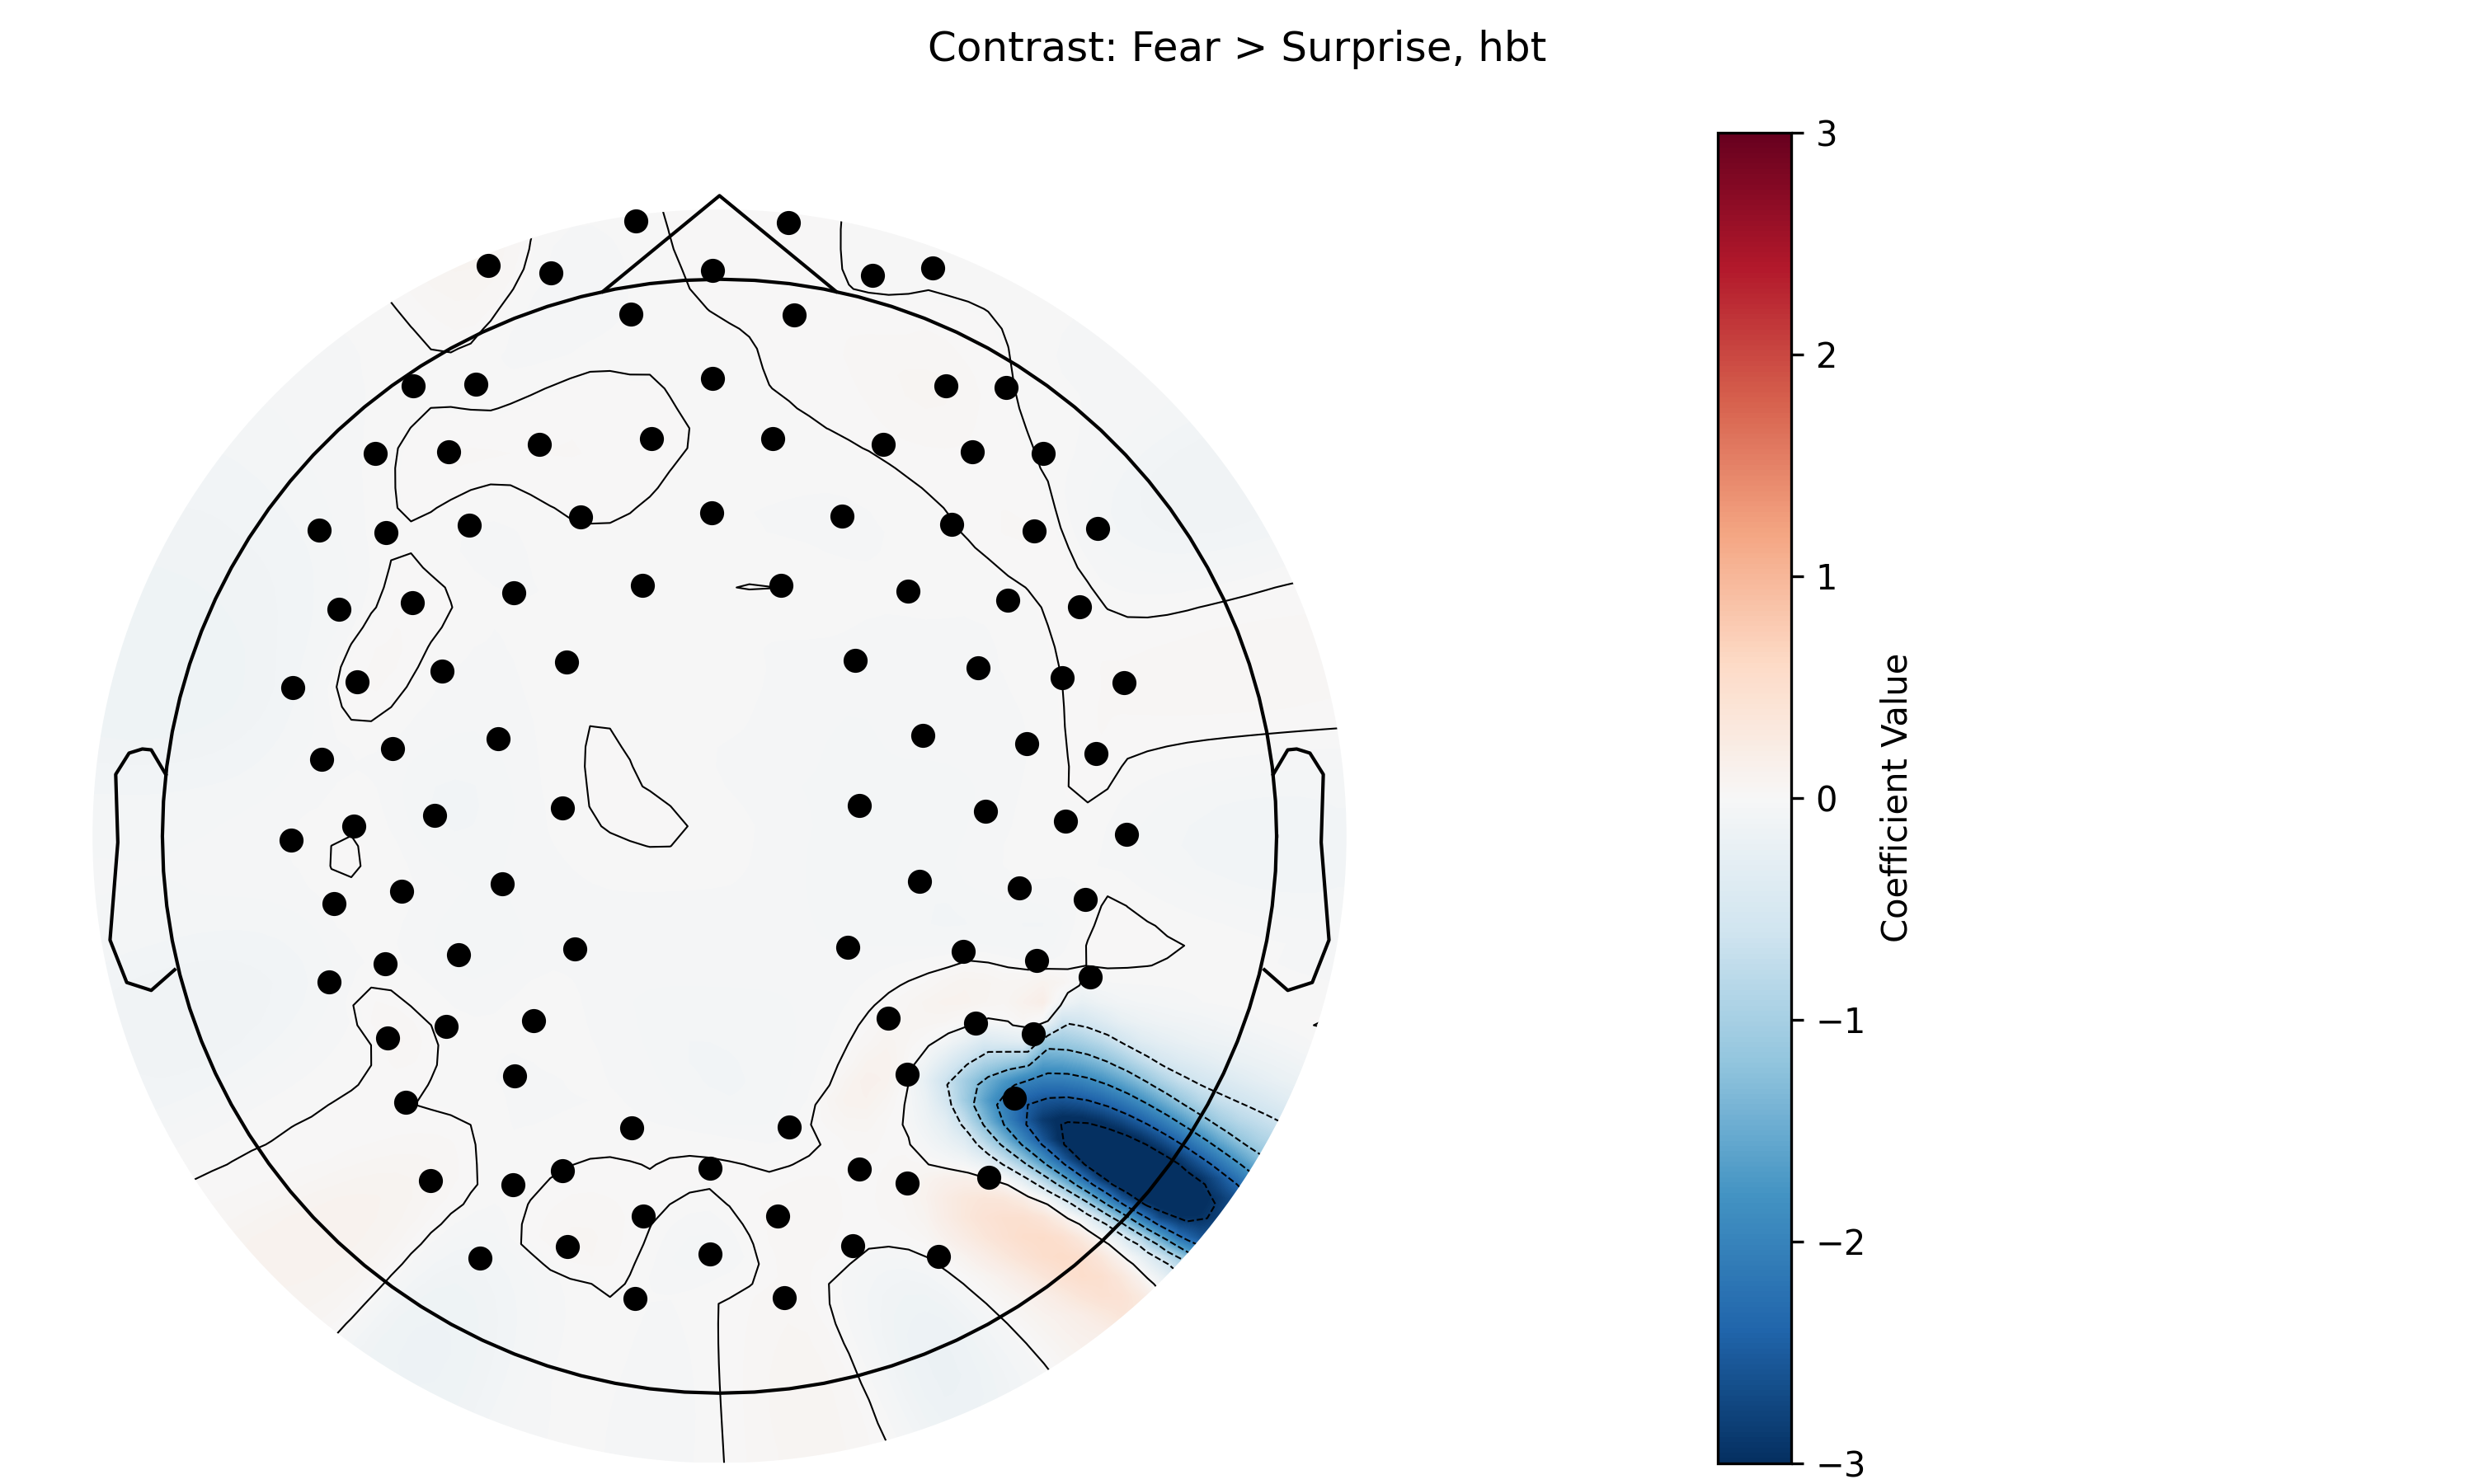
\includegraphics[width=0.45\textwidth]{C:/Users/super/OneDrive - Ontario Tech University/fNIRS_Emotions/plots/glm/contrasts/differences/Contrast_Fear-Surprise.png}
      
\includegraphics[width=0.45\textwidth]{C:/Users/super/OneDrive - Ontario Tech University/fNIRS_Emotions/plots/glm/contrasts/differences/Contrast_Joy-Surprise.png}
      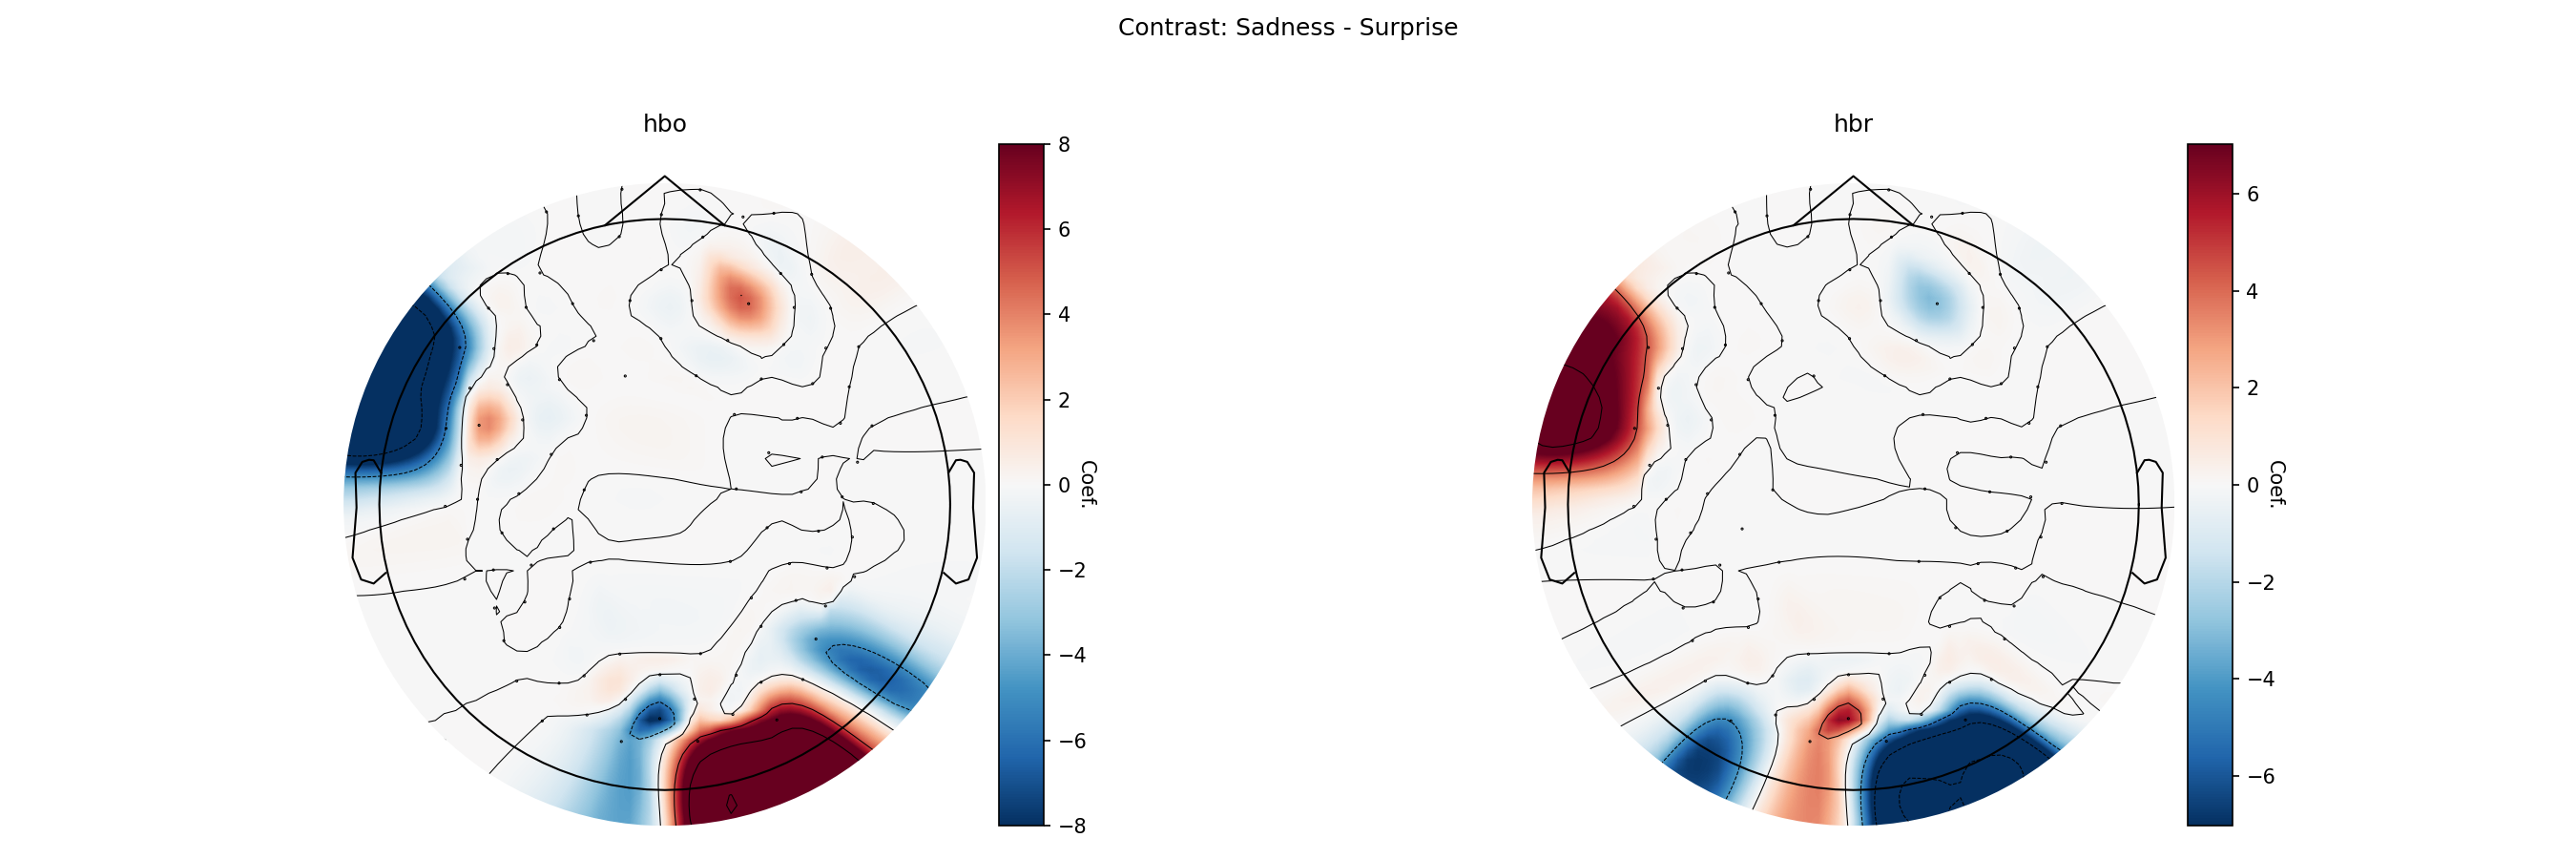
\includegraphics[width=0.45\textwidth]{C:/Users/super/OneDrive - Ontario Tech University/fNIRS_Emotions/plots/glm/contrasts/differences/Contrast_Sadness-Surprise.png}
      \caption[GLM: Emotion vs. Surprise]{GLM results for the contrast between different emotions and surprise condition.
      Same concept as explained in figure \ref{fig:glm_real_vs_virtual}. }
      \label{fig:glm_emotion_analysis_surprise}
\end{figure}

When comparing each emotion against Surprise (as shown in \ref{fig:glm_emotion_analysis_surprise}), significant differences in activation were observed across multiple brain regions. 
Disgust and Joy both showed decreased activation in the right occipital and left prefrontal regions relative to Surprise. 
Fear was associated with reduced activation in the right parietal region, while Sadness showed decreased activation in both the left frontal and right parietal regions. 
These findings suggest that each emotion, when contrasted with Surprise, elicits distinct neural activation patterns all across the brain, rather than being limited to specific regions.

\begin{figure}[H]
    \centering
      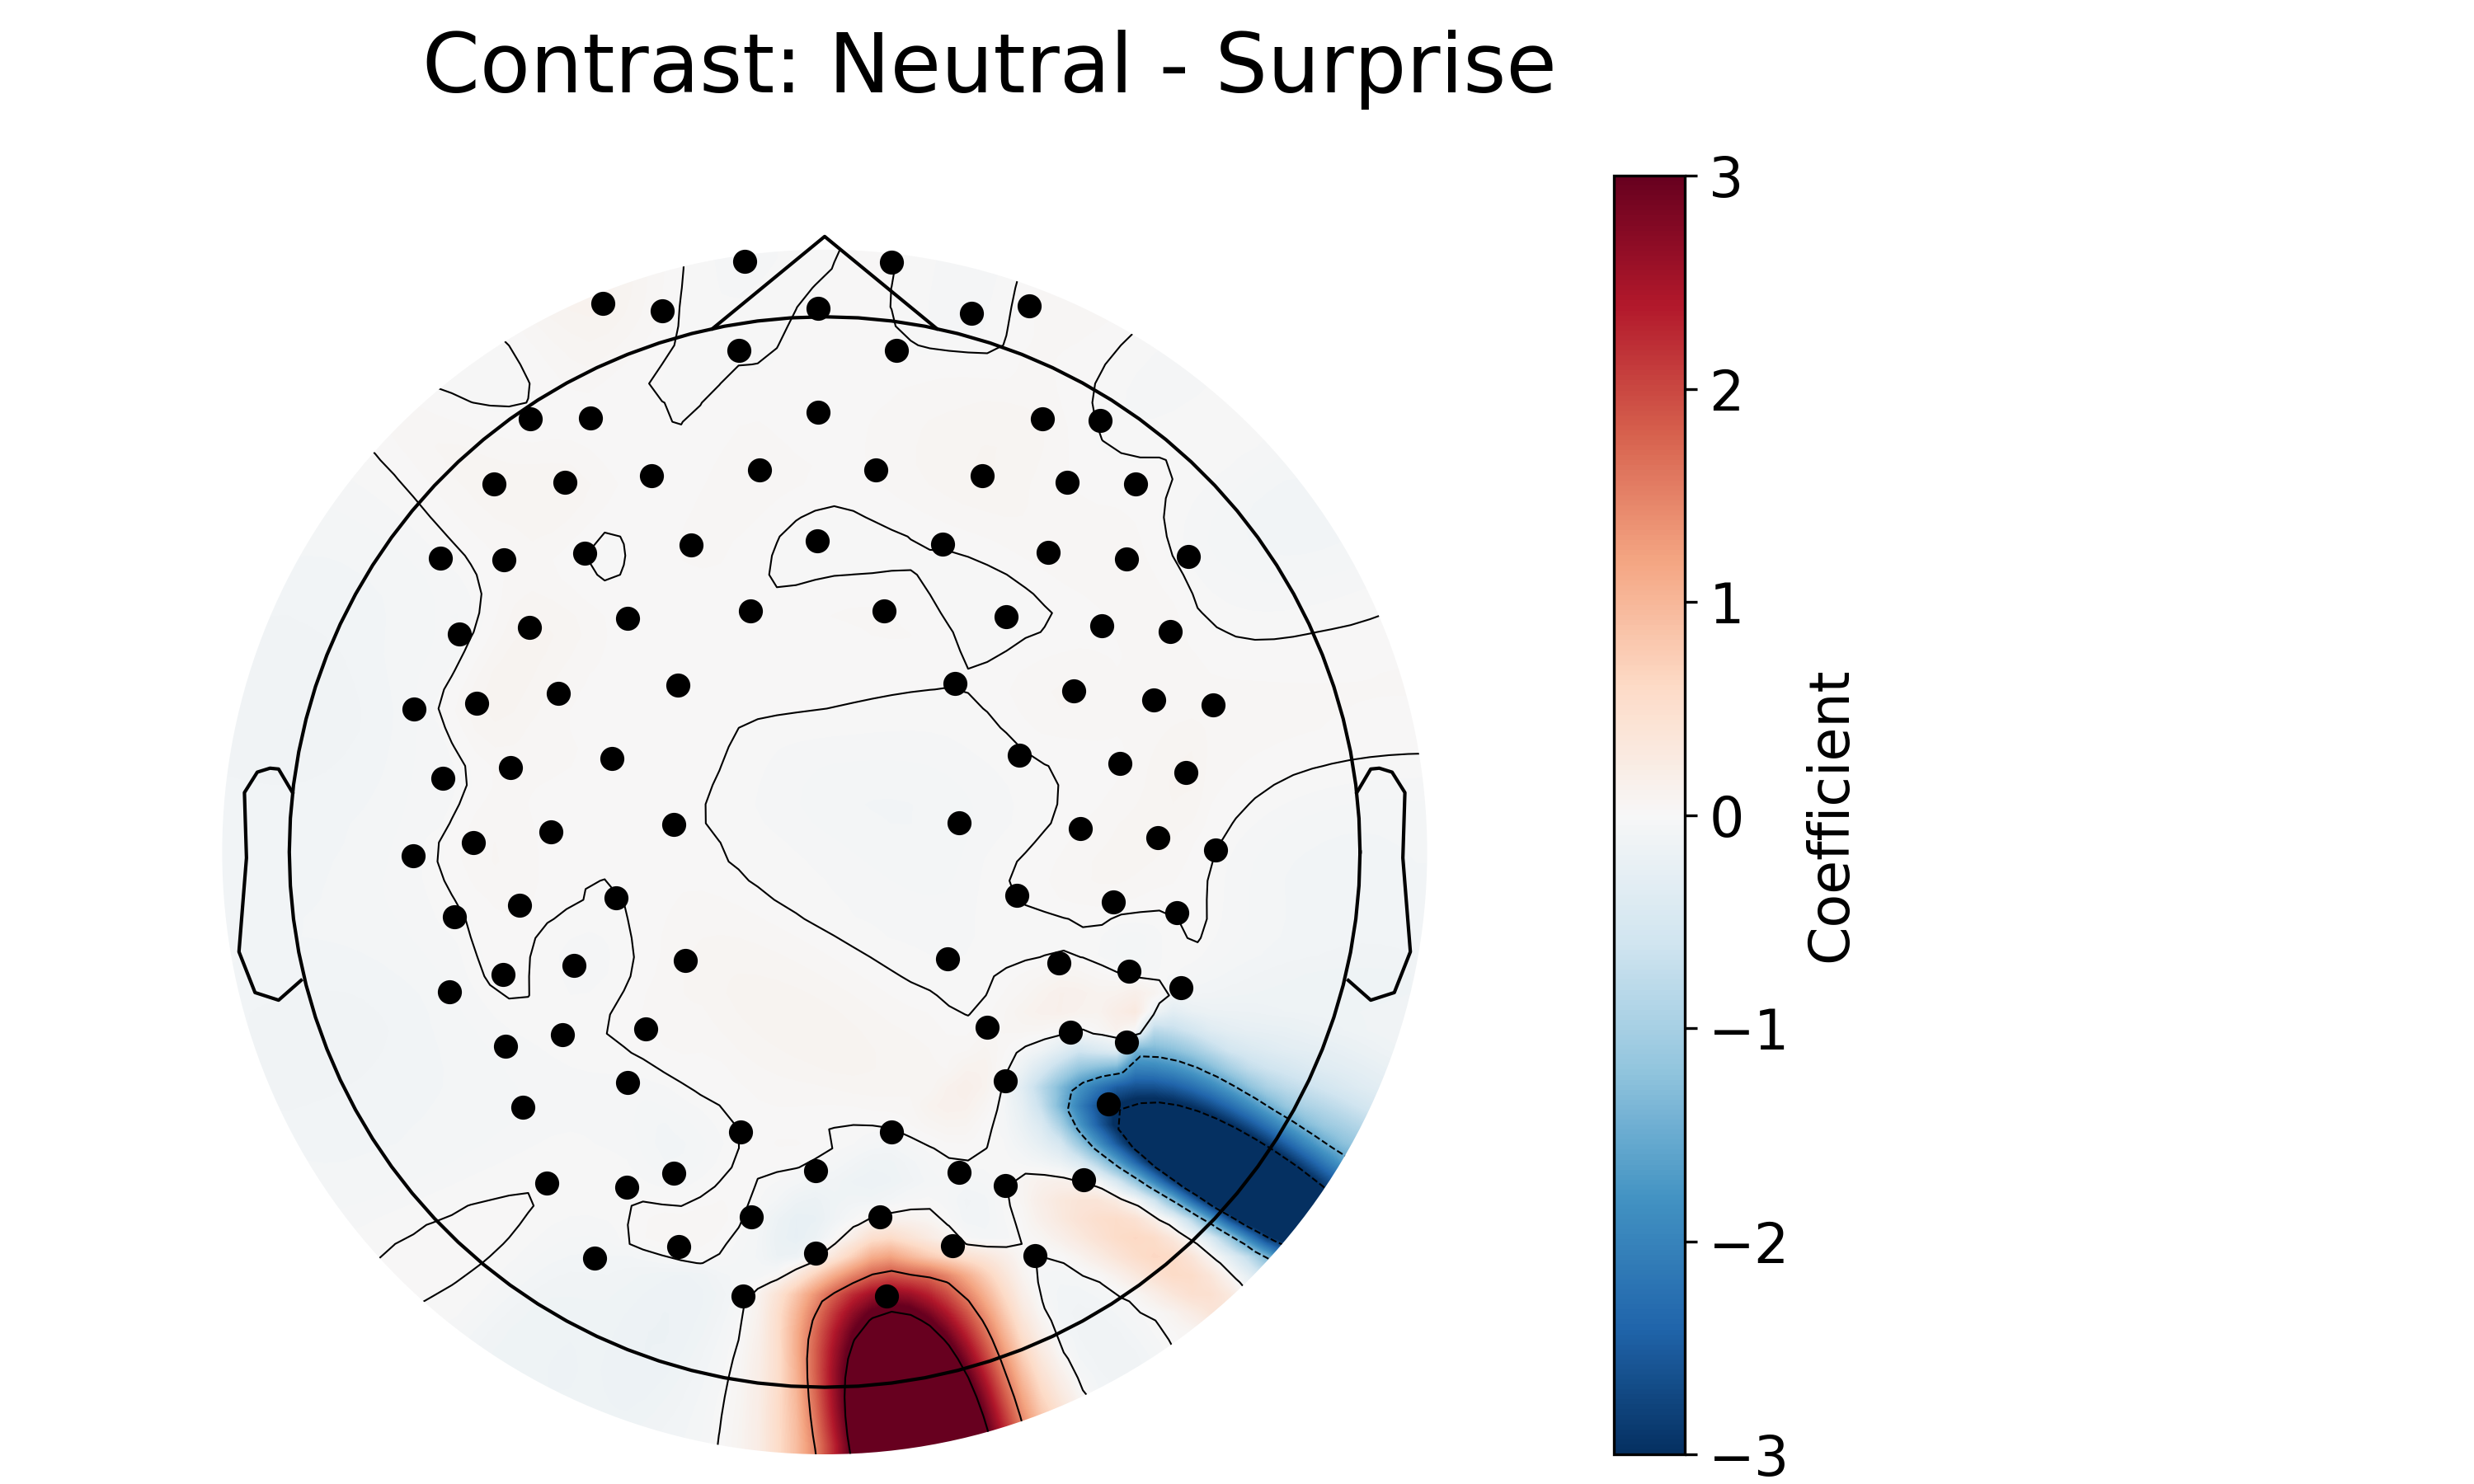
\includegraphics[width=0.85\textwidth]{C:/Users/super/OneDrive - Ontario Tech University/fNIRS_Emotions/plots/glm/contrasts/differences_neutral/Contrast_Neutral-Surprise.png}
      \caption[GLM: Neutral vs. Surprise]{GLM results for the contrast between neutral and surprise condition.
      Same concept as explained in figure \ref{fig:glm_real_vs_virtual}. }
      \label{fig:glm_neutral_vs_surprise}
\end{figure}

The Neutral $>$ Surprise comparison (as shown in \ref{fig:glm_neutral_vs_surprise}) revealed significant differences in the right parietal and right occipital regions. 
The right parietal region showed decreased activation (more activation for Surprise) while the right occipital region showed increased activation (more activation for neutral).
Both Neutral and Surprise conditions elicit greater activation when compared to the other emotions, but when compared to each other, one emotion is not more activated than the other.
This indicates that the neural response to Neutral and Surprise conditions is distinct, with each condition eliciting different activation patterns in specific brain regions.
Note that all combinations of emotion contrasts were performed, no other significant differences were found between any other emotions than the ones shown in this section.

\subsection{Face Type \texorpdfstring{$\times$}{x} Emotion Contrasts}
\begin{figure}[H]
  \centering
  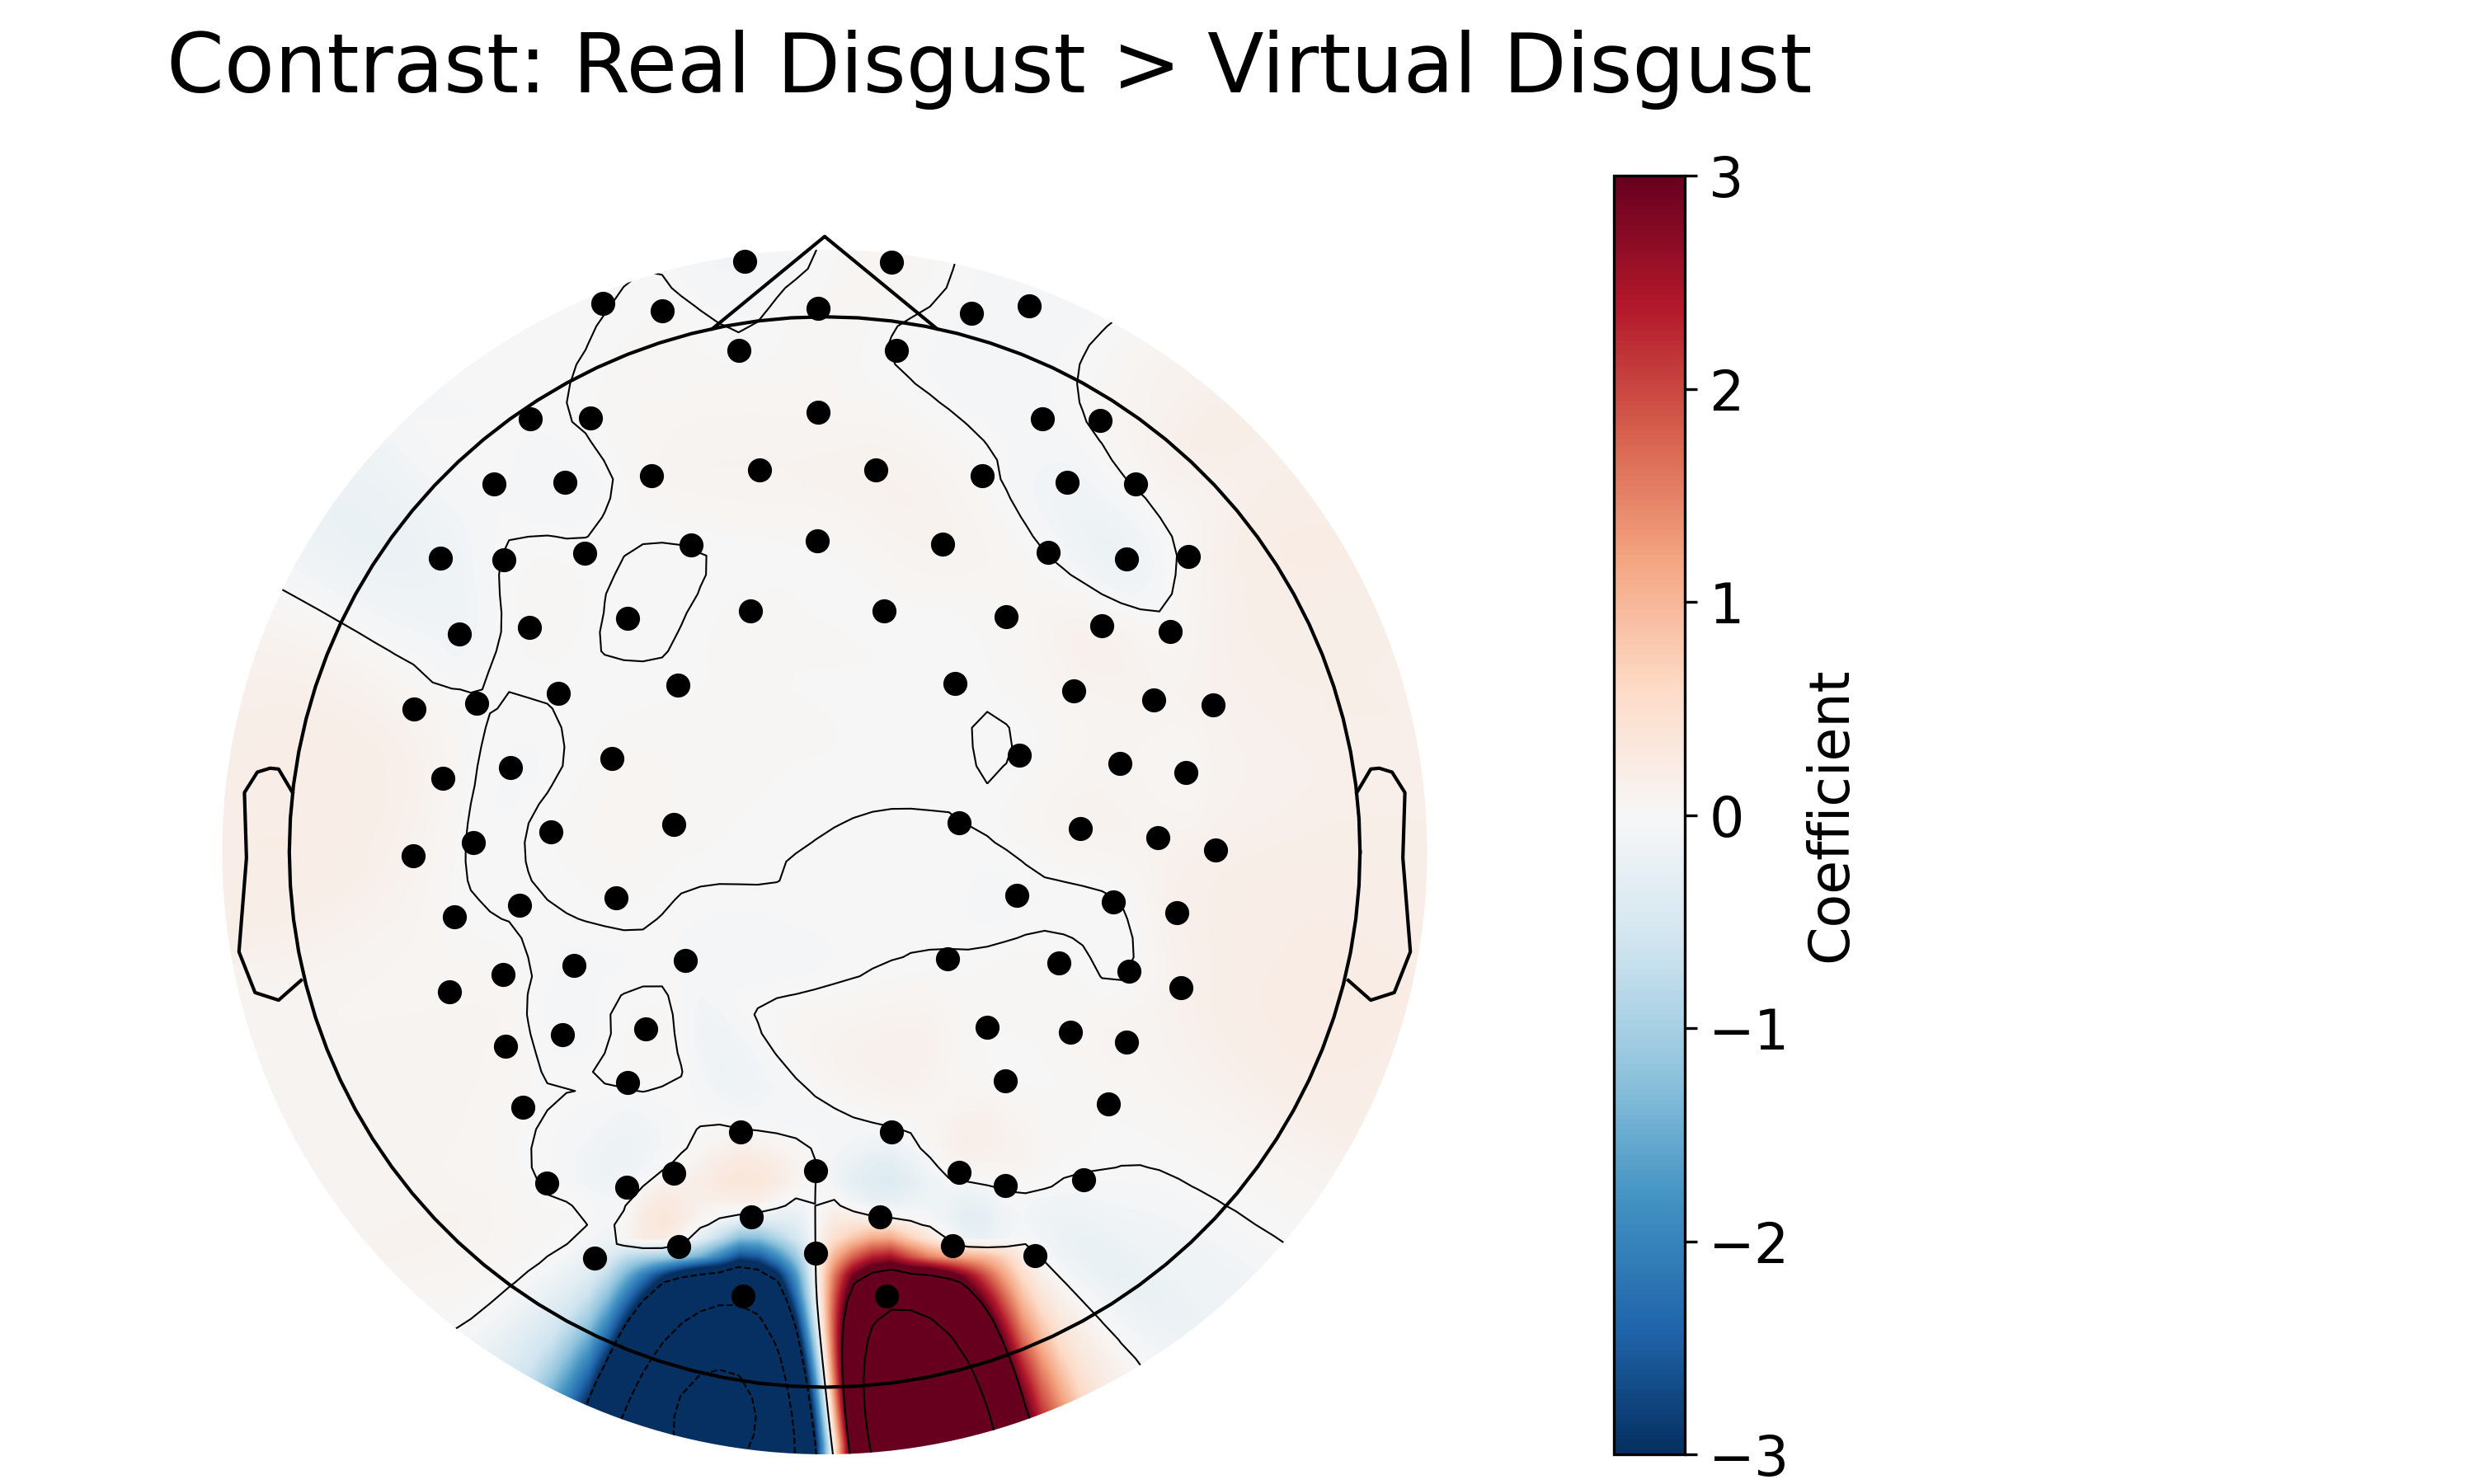
\includegraphics[width=0.45\textwidth]{C:/Users/super/OneDrive - Ontario Tech University/fNIRS_Emotions/plots/glm/contrasts/differences/Contrast_Real_Disgust-Virt_Disgust.png}
  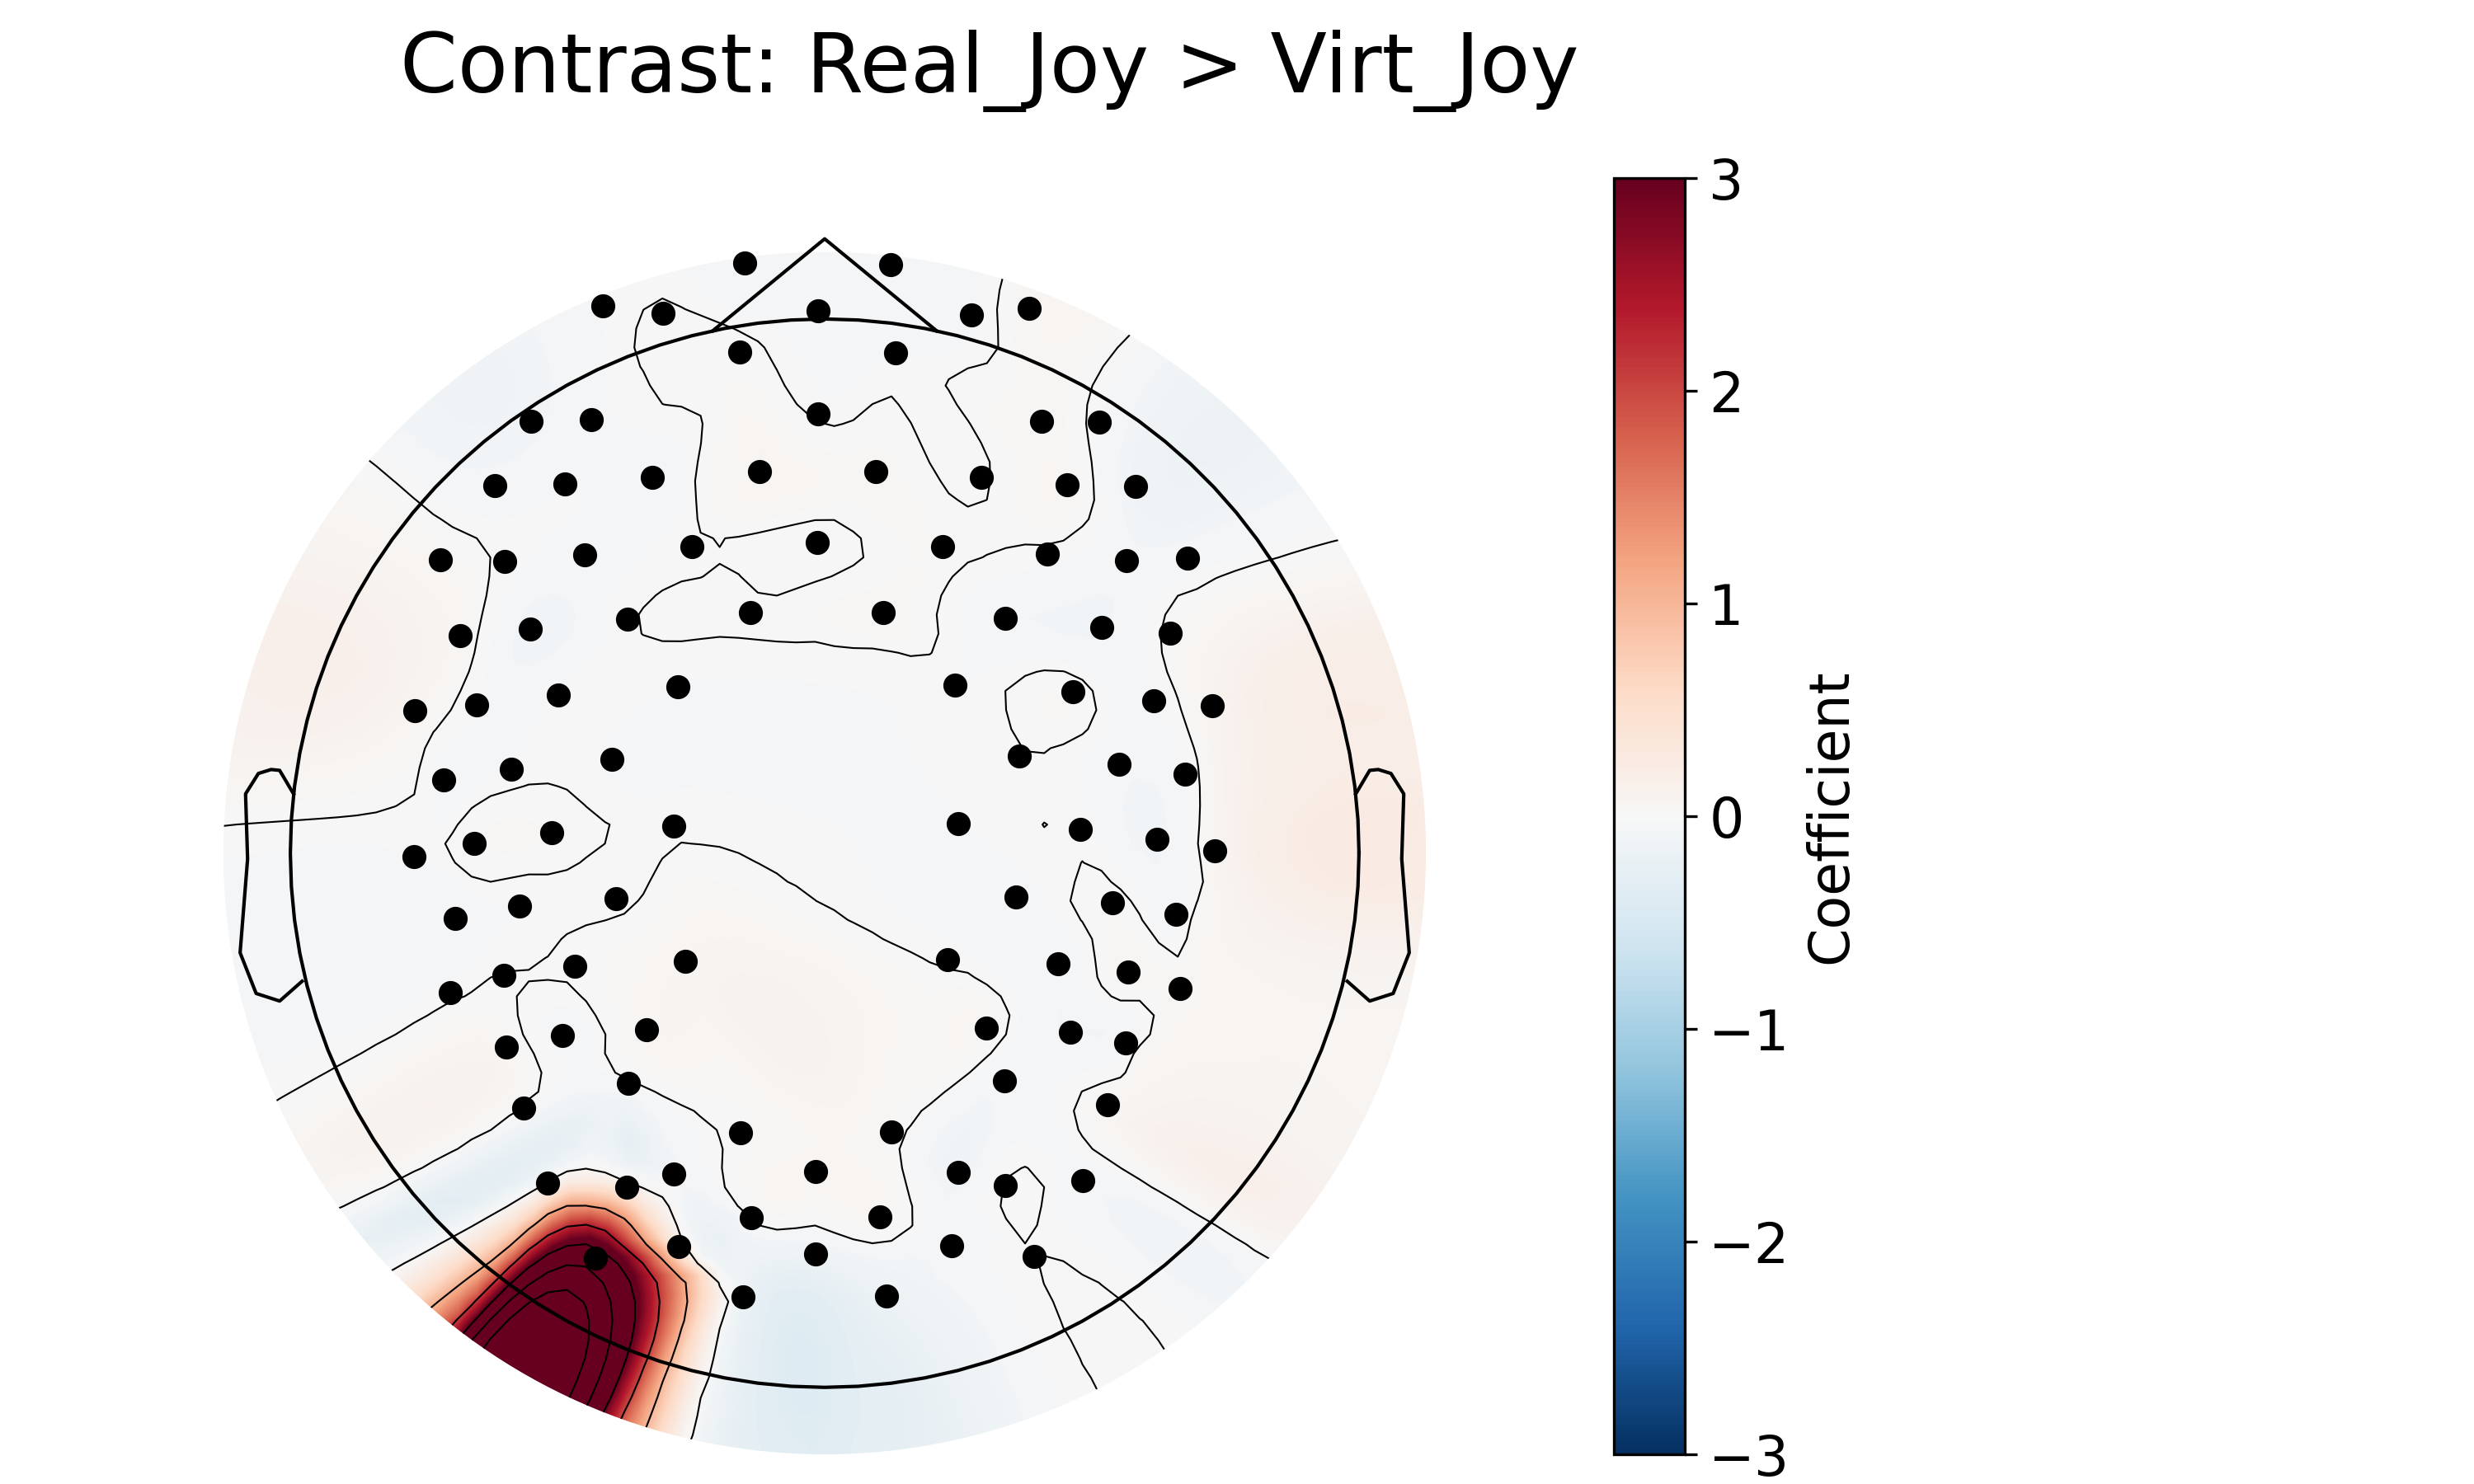
\includegraphics[width=0.45\textwidth]{C:/Users/super/OneDrive - Ontario Tech University/fNIRS_Emotions/plots/glm/contrasts/differences/Contrast_Real_Joy-Virt_Joy.png}
  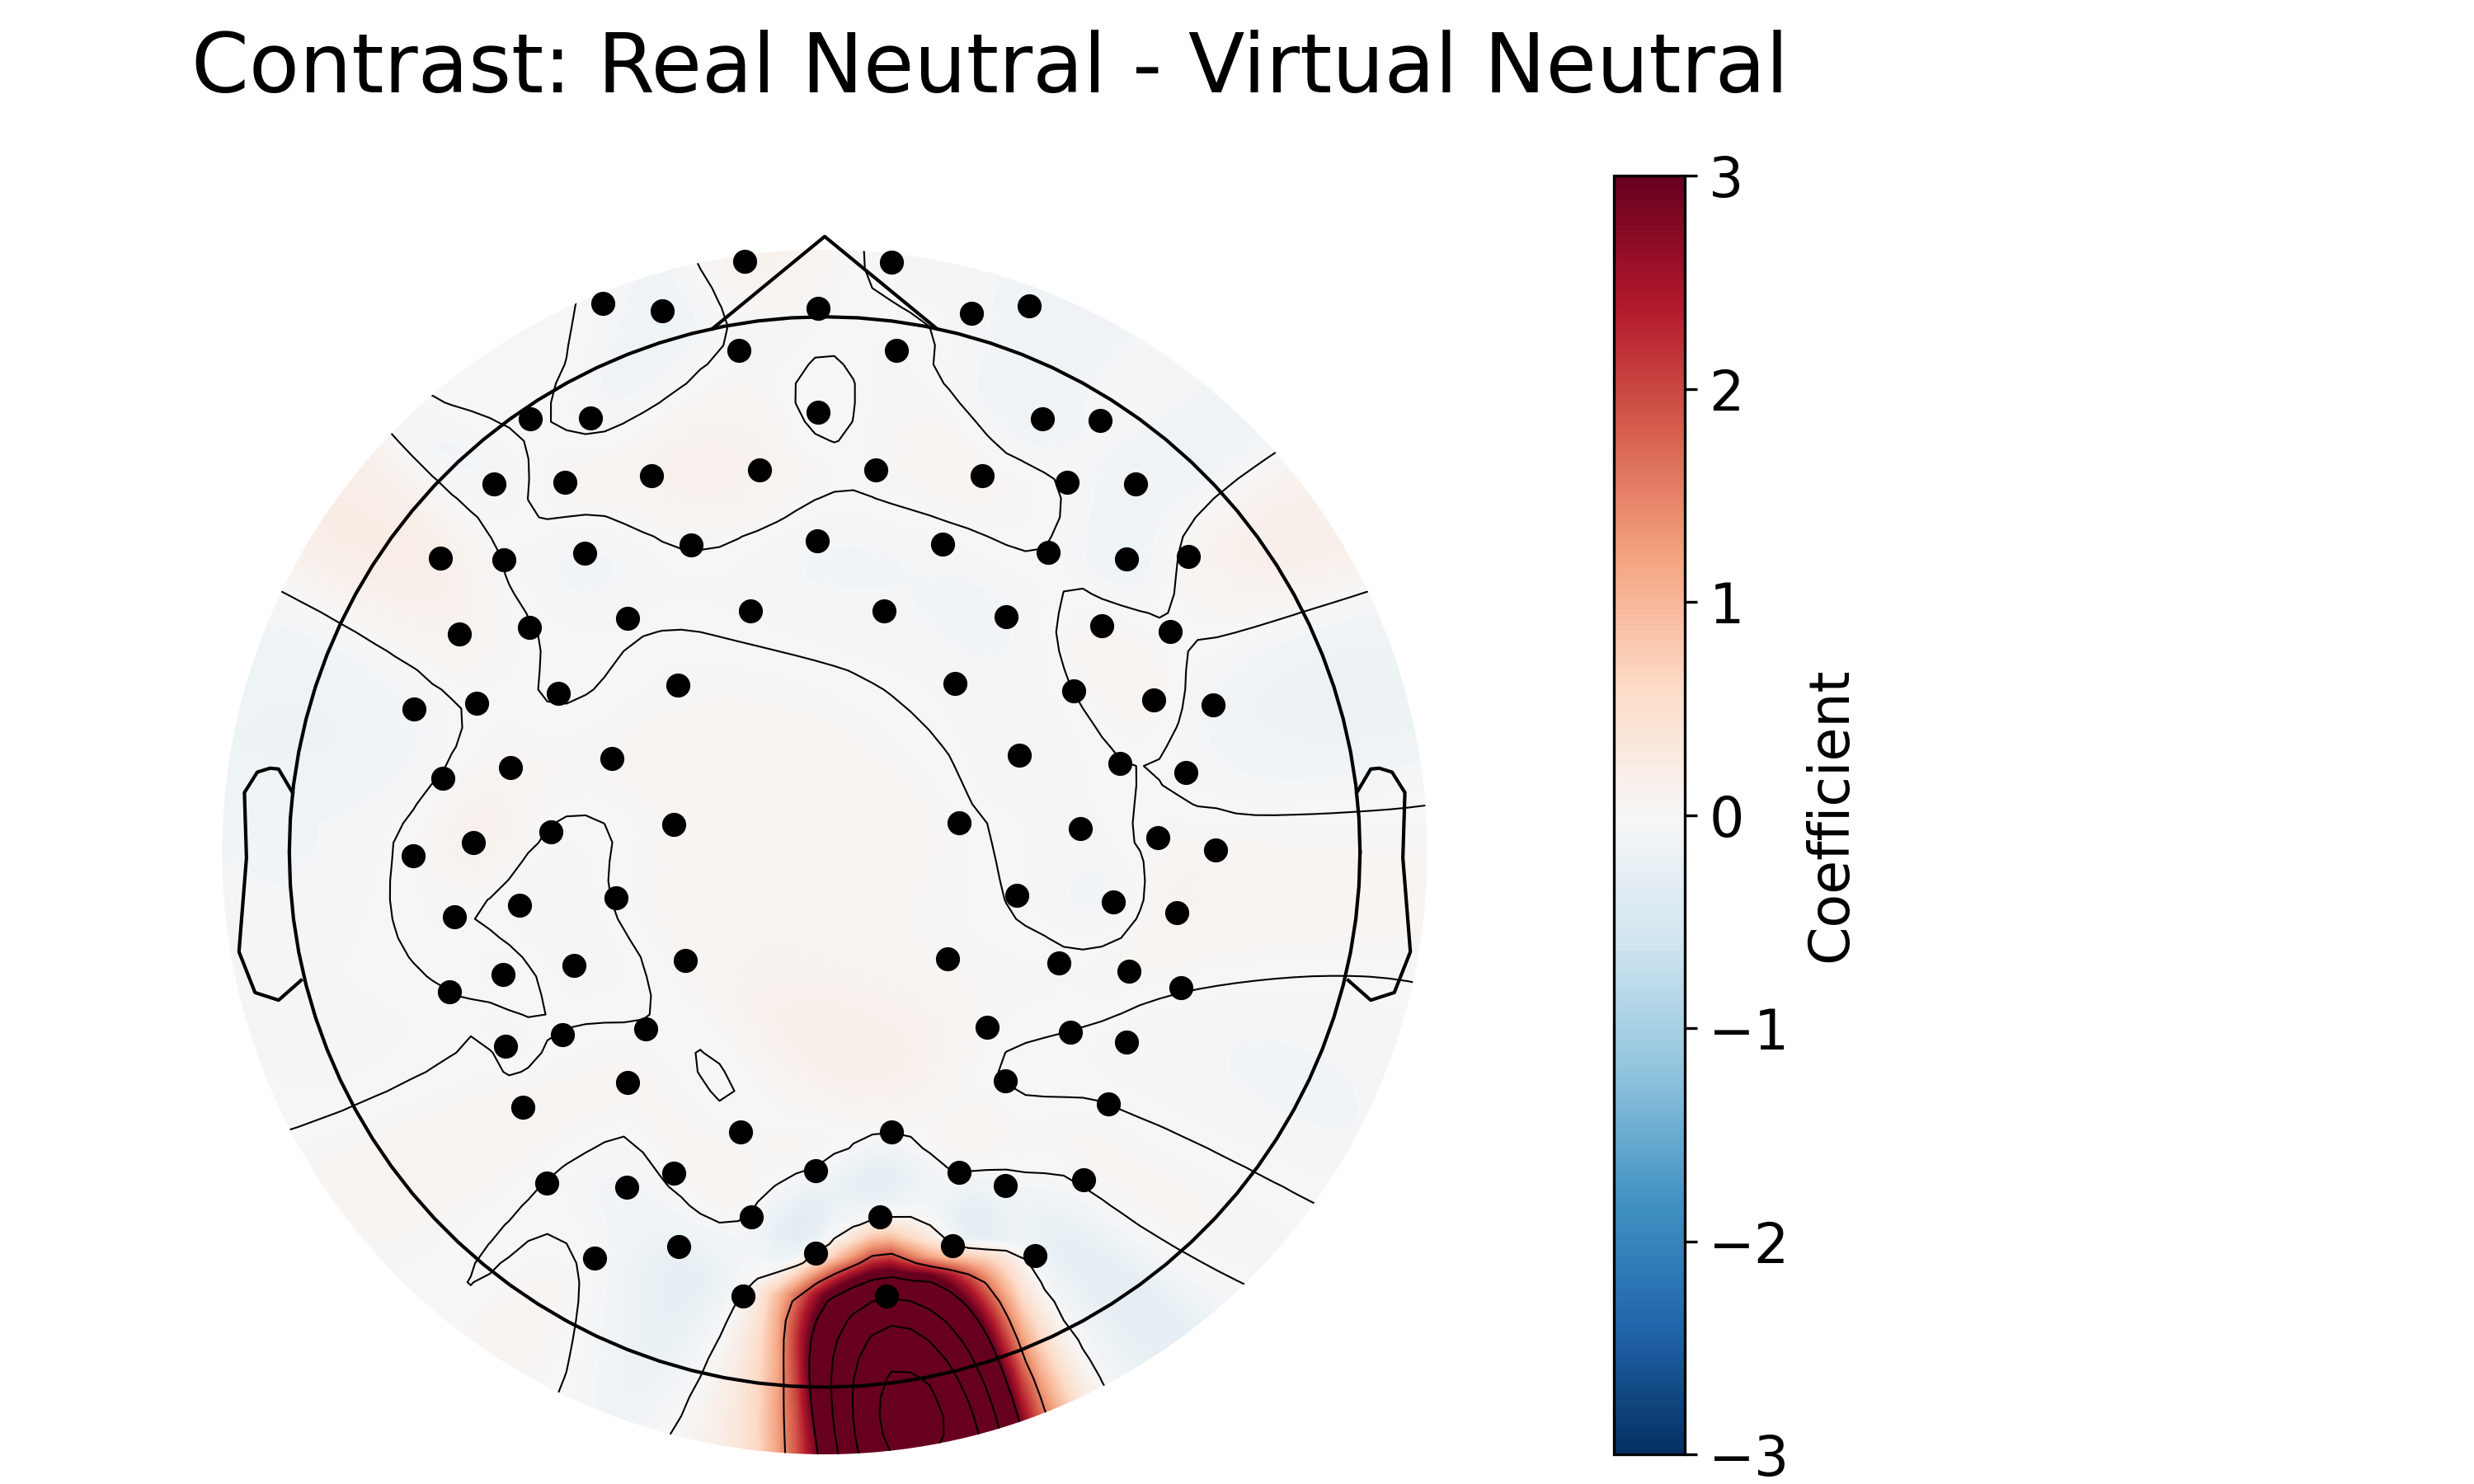
\includegraphics[width=0.45\textwidth]{C:/Users/super/OneDrive - Ontario Tech University/fNIRS_Emotions/plots/glm/contrasts/differences/Contrast_Real_Neutral-Virt_Neutral.png}
  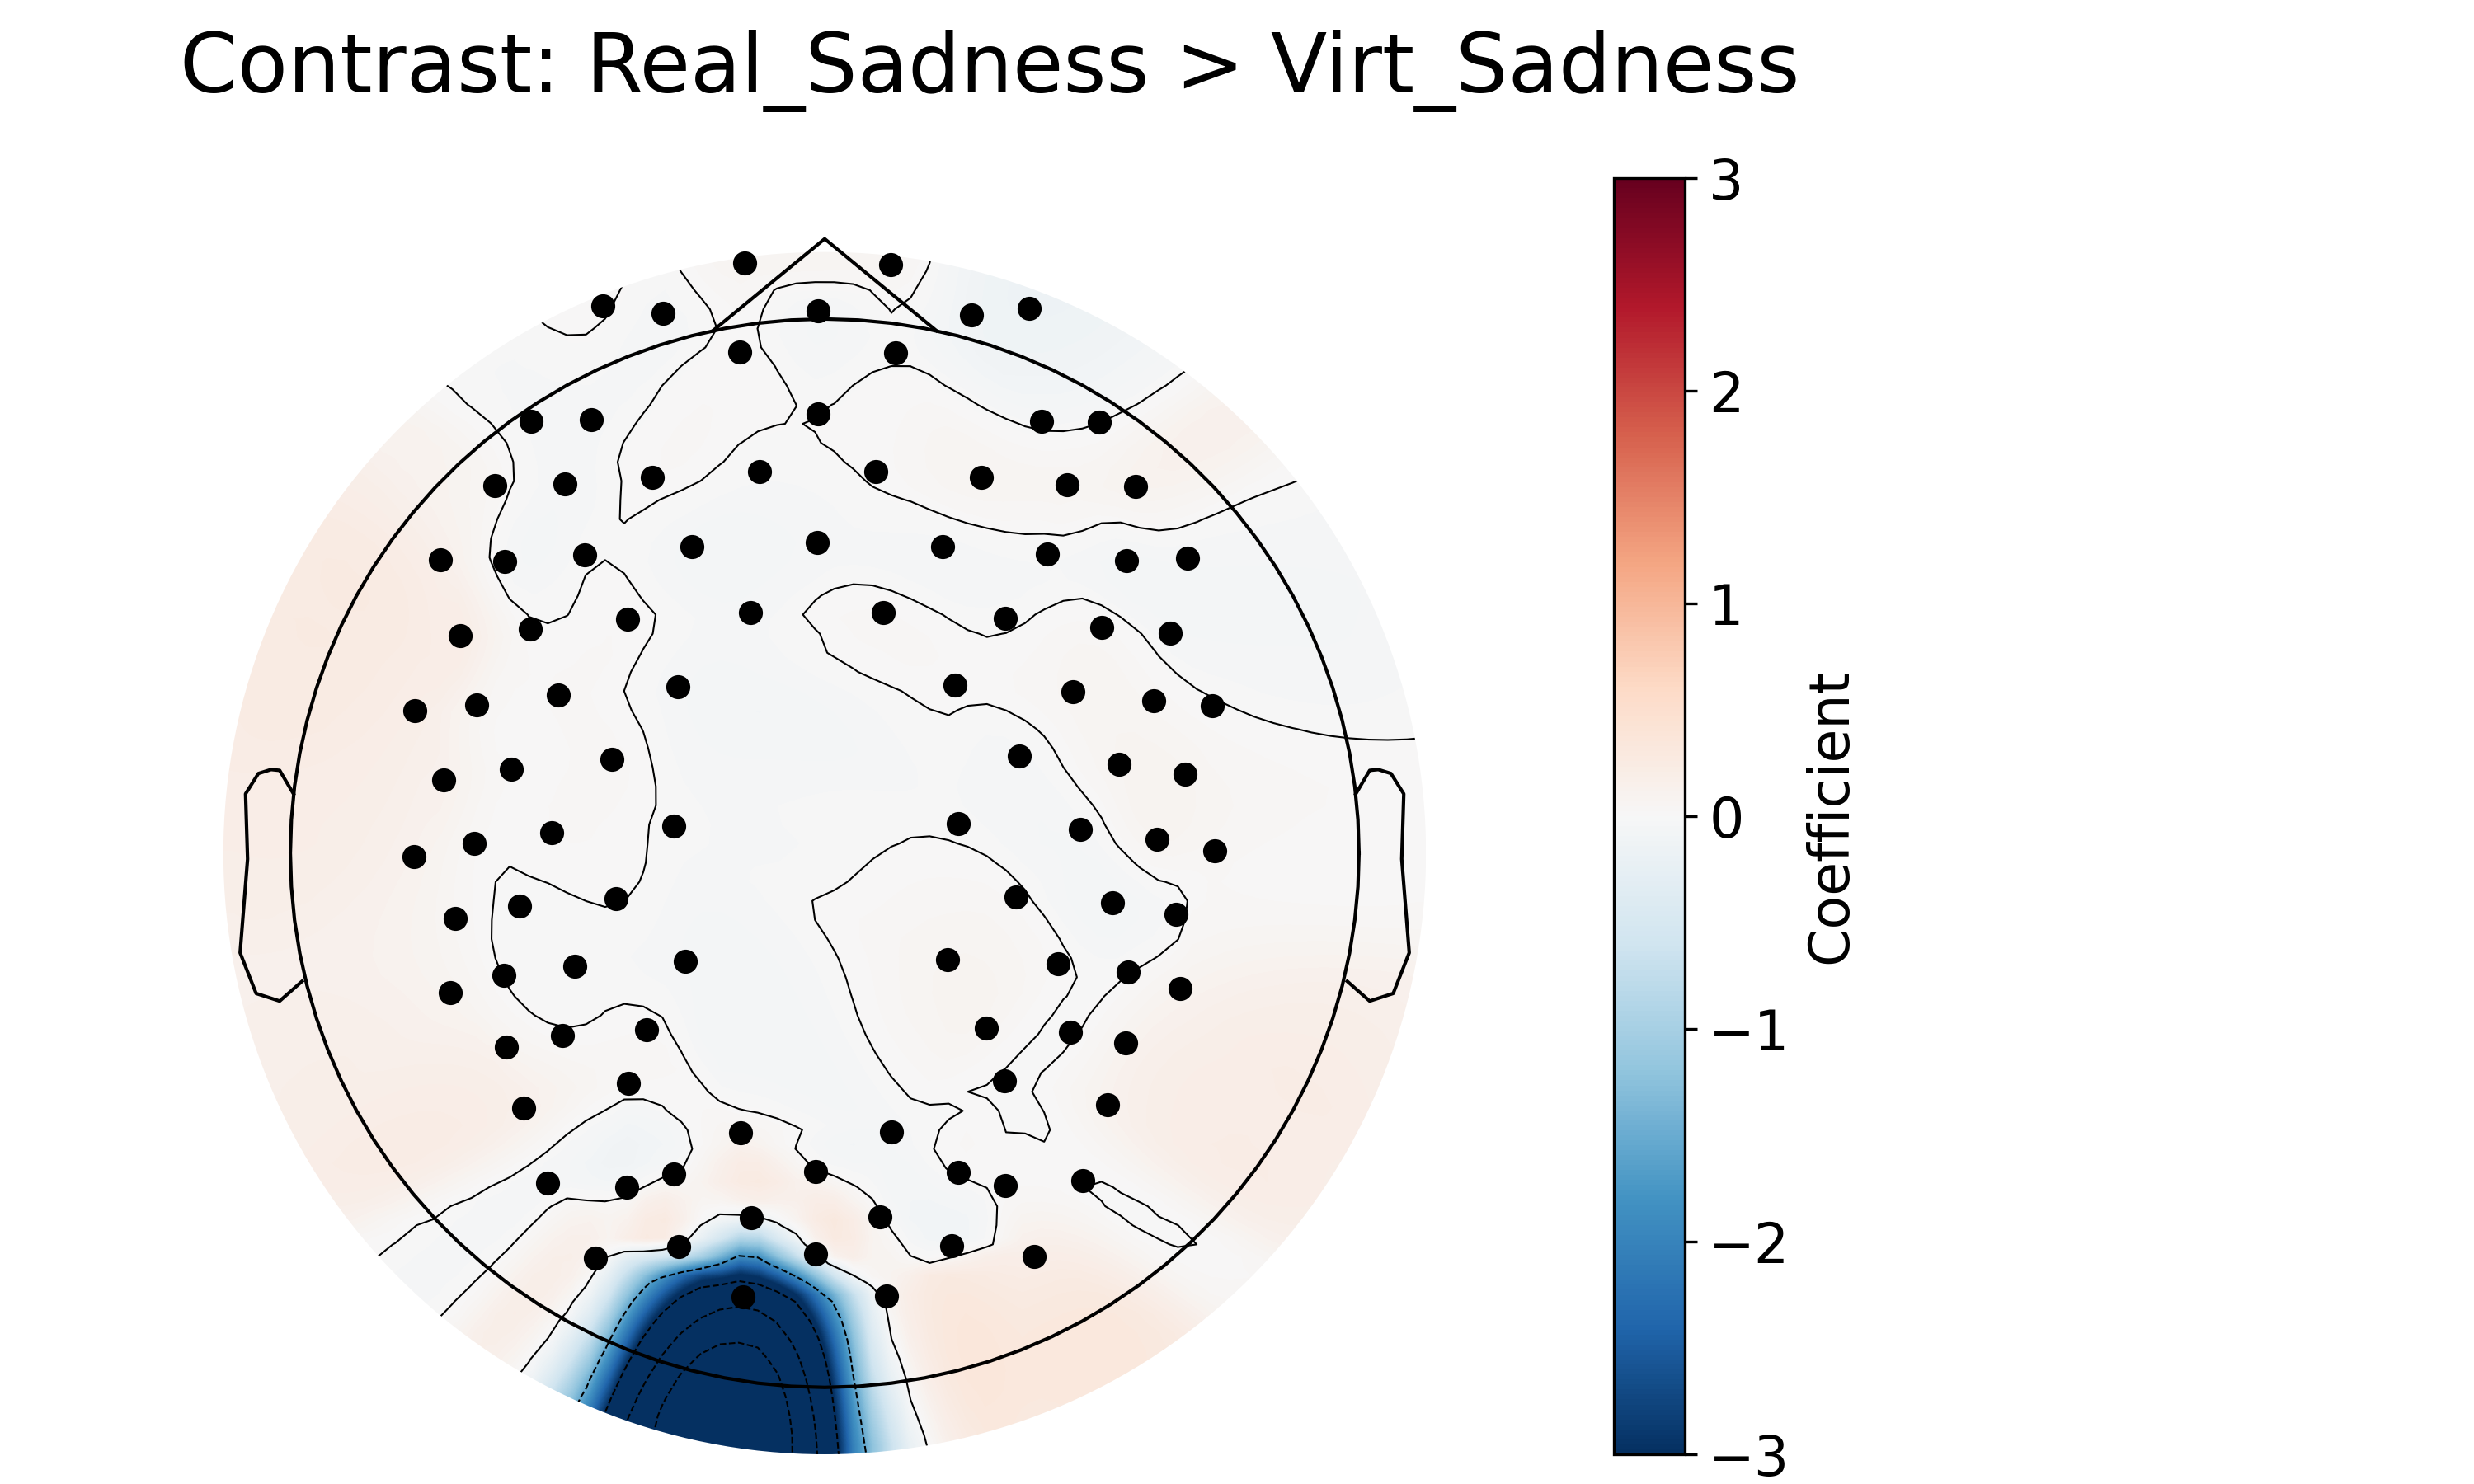
\includegraphics[width=0.45\textwidth]{C:/Users/super/OneDrive - Ontario Tech University/fNIRS_Emotions/plots/glm/contrasts/differences/Contrast_Real_Sadness-Virt_Sadness.png}
  \caption[GLM: Face Type \texorpdfstring{$\times$}{x} Emotion Contrasts]{GLM results for the contrast between real and virtual conditions within each emotion.
  Same concept as explained in figure \ref{fig:glm_real_vs_virtual}. }
  \label{fig:glm_real_vs_virtual_emotion_analysis}
\end{figure}

The interaction of face type with emotion (Real $>$ Virt within each emotion as shown in \ref{fig:glm_real_vs_virtual_emotion_analysis}) revealed significant differences in occipital regions exclusively.
In the case of disgust, real faces elicited greater activation in the right occipital region compared to virtual faces, while the left occipital region showed the opposite pattern.
For Joy and Neutral emotions, real faces also elicited greater activation in the occipital regions compared to virtual faces.
For Sadness, the left occipital region showed greater activation for virtual faces compared to real faces.
These findings suggest that the neural response to emotional expressions is modulated by the realism of the face stimuli. 

The full table of the GLM contrasts for all main effects and interactions can be found in Appendix \ref{tab:appendix_glm_results}.

\section{Functional Connectivity Results}
\subsection{Face Type Contrasts}
\begin{figure}[H]
  \centering
  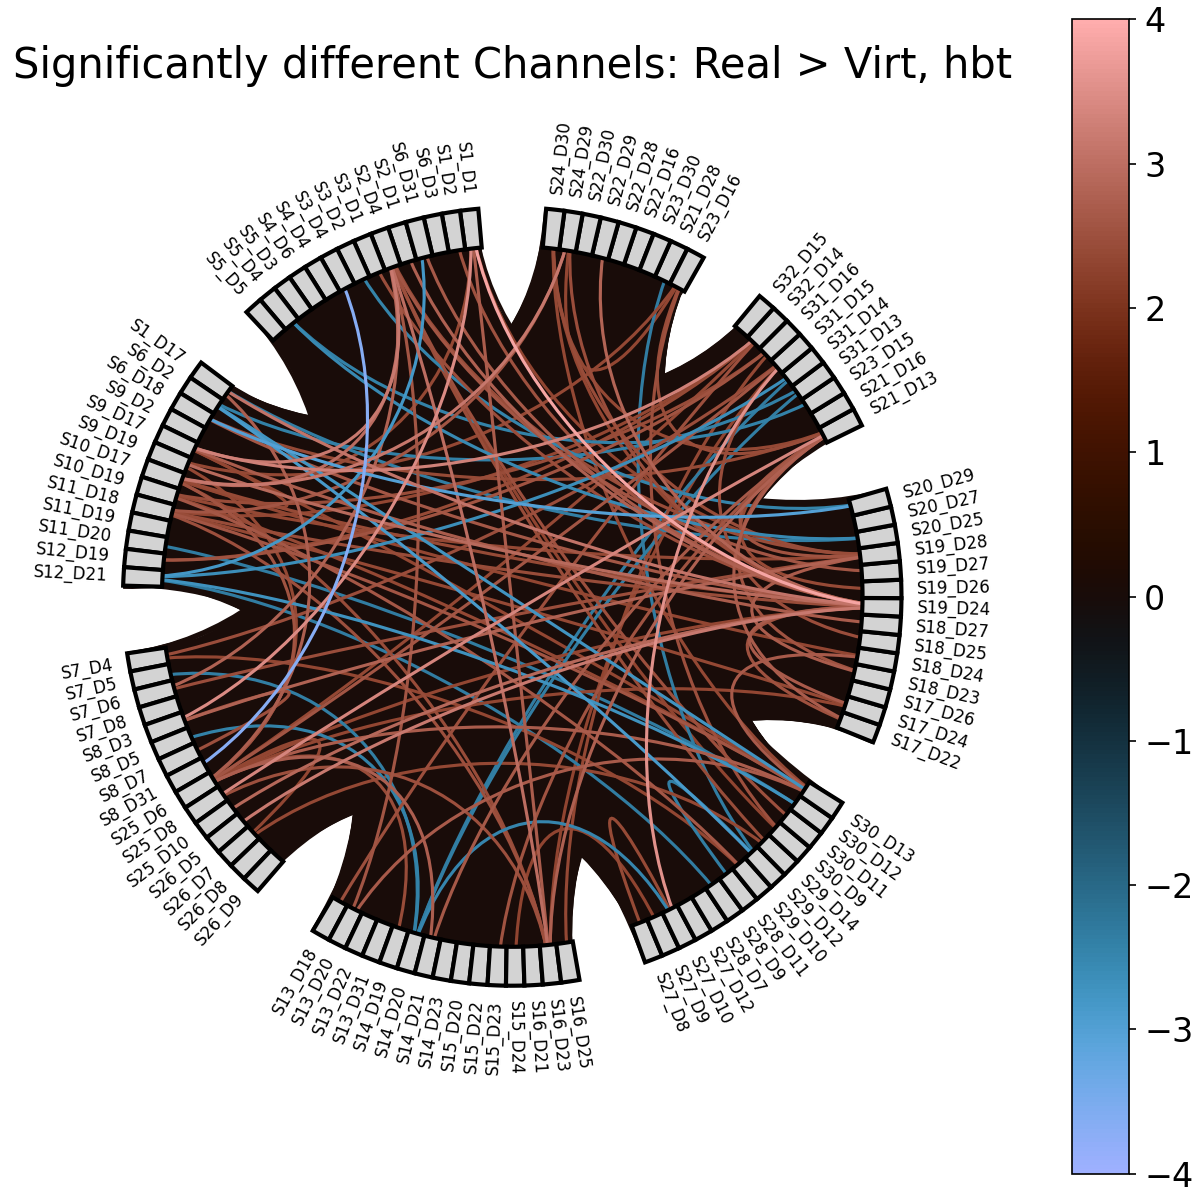
\includegraphics[width=0.85\textwidth]{C:/Users/super/OneDrive - Ontario Tech University/fNIRS_Emotions/plots/spectral_connectivity_time/chord_plots/group_level_t_tests_roi/face_type_Real_Virt.png}
  \caption[FC: Real vs. Virtual]{Functional connectivity results for the contrast between real and virtual conditions.
  Red signifies that condition 1 (real faces) has higher connectivity between those two ROI's than condition 2 (virtual faces), while blue signifies that condition 2 (virtual faces) has higher connectivity than condition 1 (real faces).
  The color bar on the right shows the $t$-statistic of the contrast, which indicates the strength of the difference in connectivity between the two conditions.
  The Mean $t$-value across ROI's is the average of the $t$-values for all significant channel pairs across all ROI's, and generally indicates whether the connectivity is higher or lower in one condition compared to the other.
  If this value is positive, it indicates that the connectivity is higher in condition 1 (real faces) than condition 2 (virtual faces), and vice versa.}
  \label{fig:fc_real_vs_virtual}
\end{figure}

The main effect of real versus virtual faces (as shown in \ref{fig:fc_real_vs_virtual}) for functional connectivity revealed significant differences in connectivity between real and virtual faces across ROI's.
Most ROI's showed higher connectivity for real faces compared to virtual faces, with a few exceptions, i.e. the left occipital/parietal ROI, which showed higher connectivity for virtual faces compared to real faces.
A mean $t$-value of 1.55 indicates that the connectivity is generally higher for real faces compared to virtual faces across all ROI's. 

\subsection{Emotion Contrasts}
\begin{figure}[H]
  \centering
  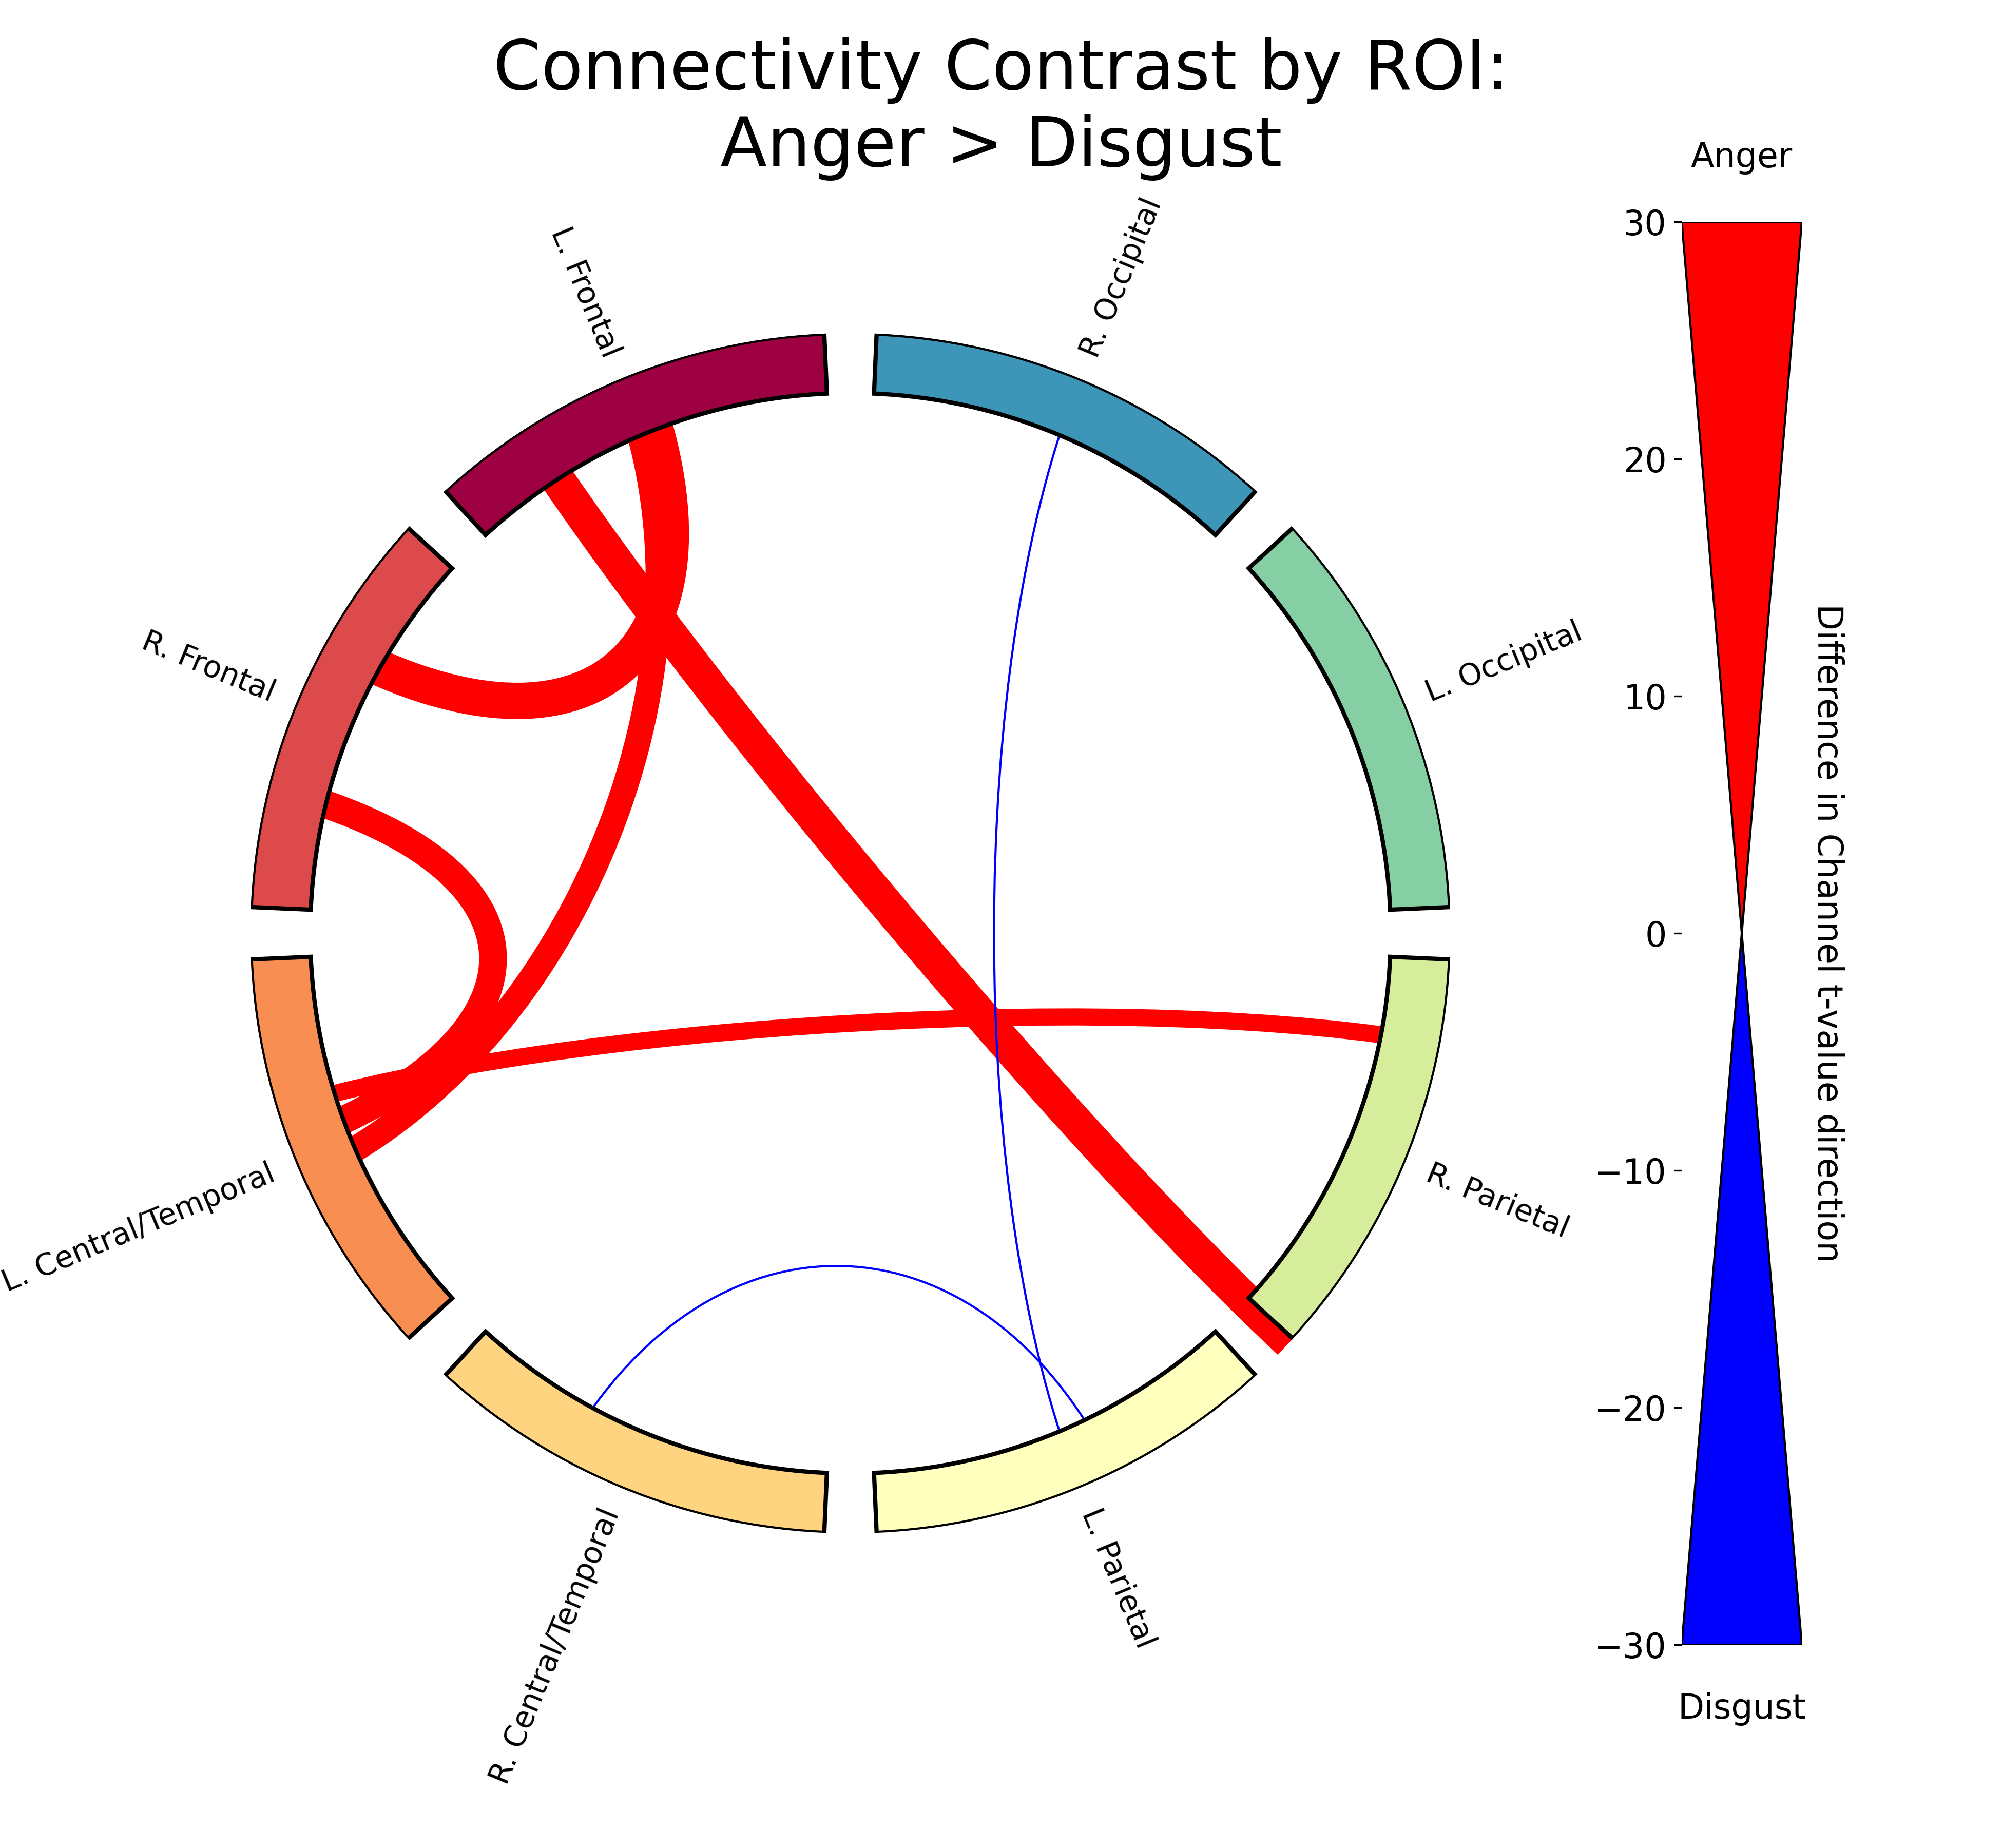
\includegraphics[width=0.24\textwidth]{C:/Users/super/OneDrive - Ontario Tech University/fNIRS_Emotions/plots/spectral_connectivity_time/chord_plots/group_level_t_tests_roi/emotion_Anger_Disgust.png}
  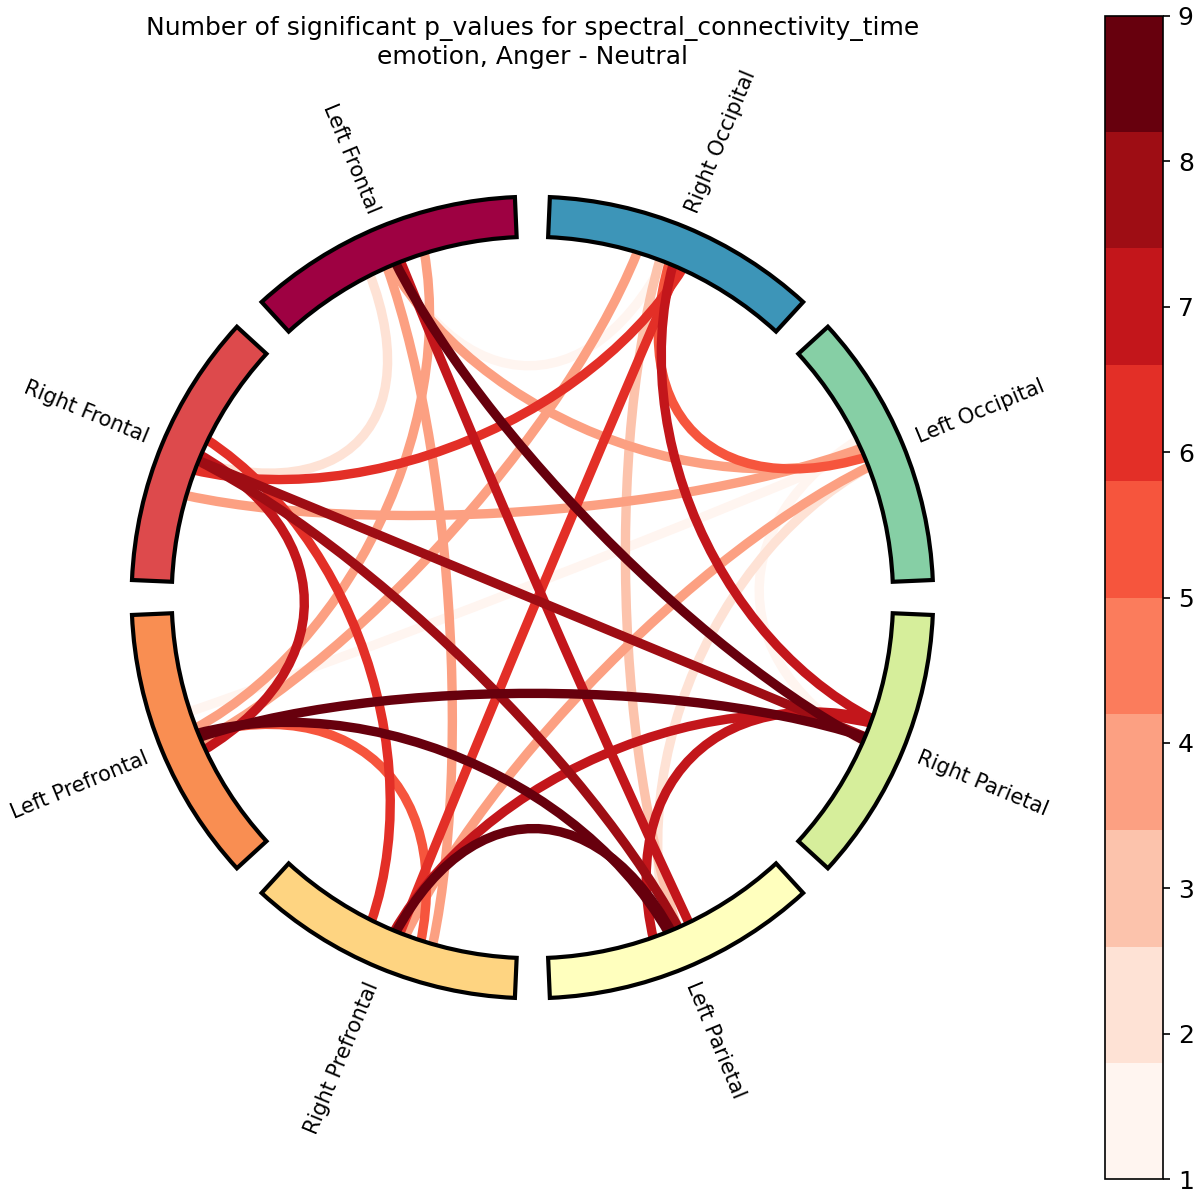
\includegraphics[width=0.24\textwidth]{C:/Users/super/OneDrive - Ontario Tech University/fNIRS_Emotions/plots/spectral_connectivity_time/chord_plots/group_level_t_tests_roi/emotion_Anger_Neutral.png}
  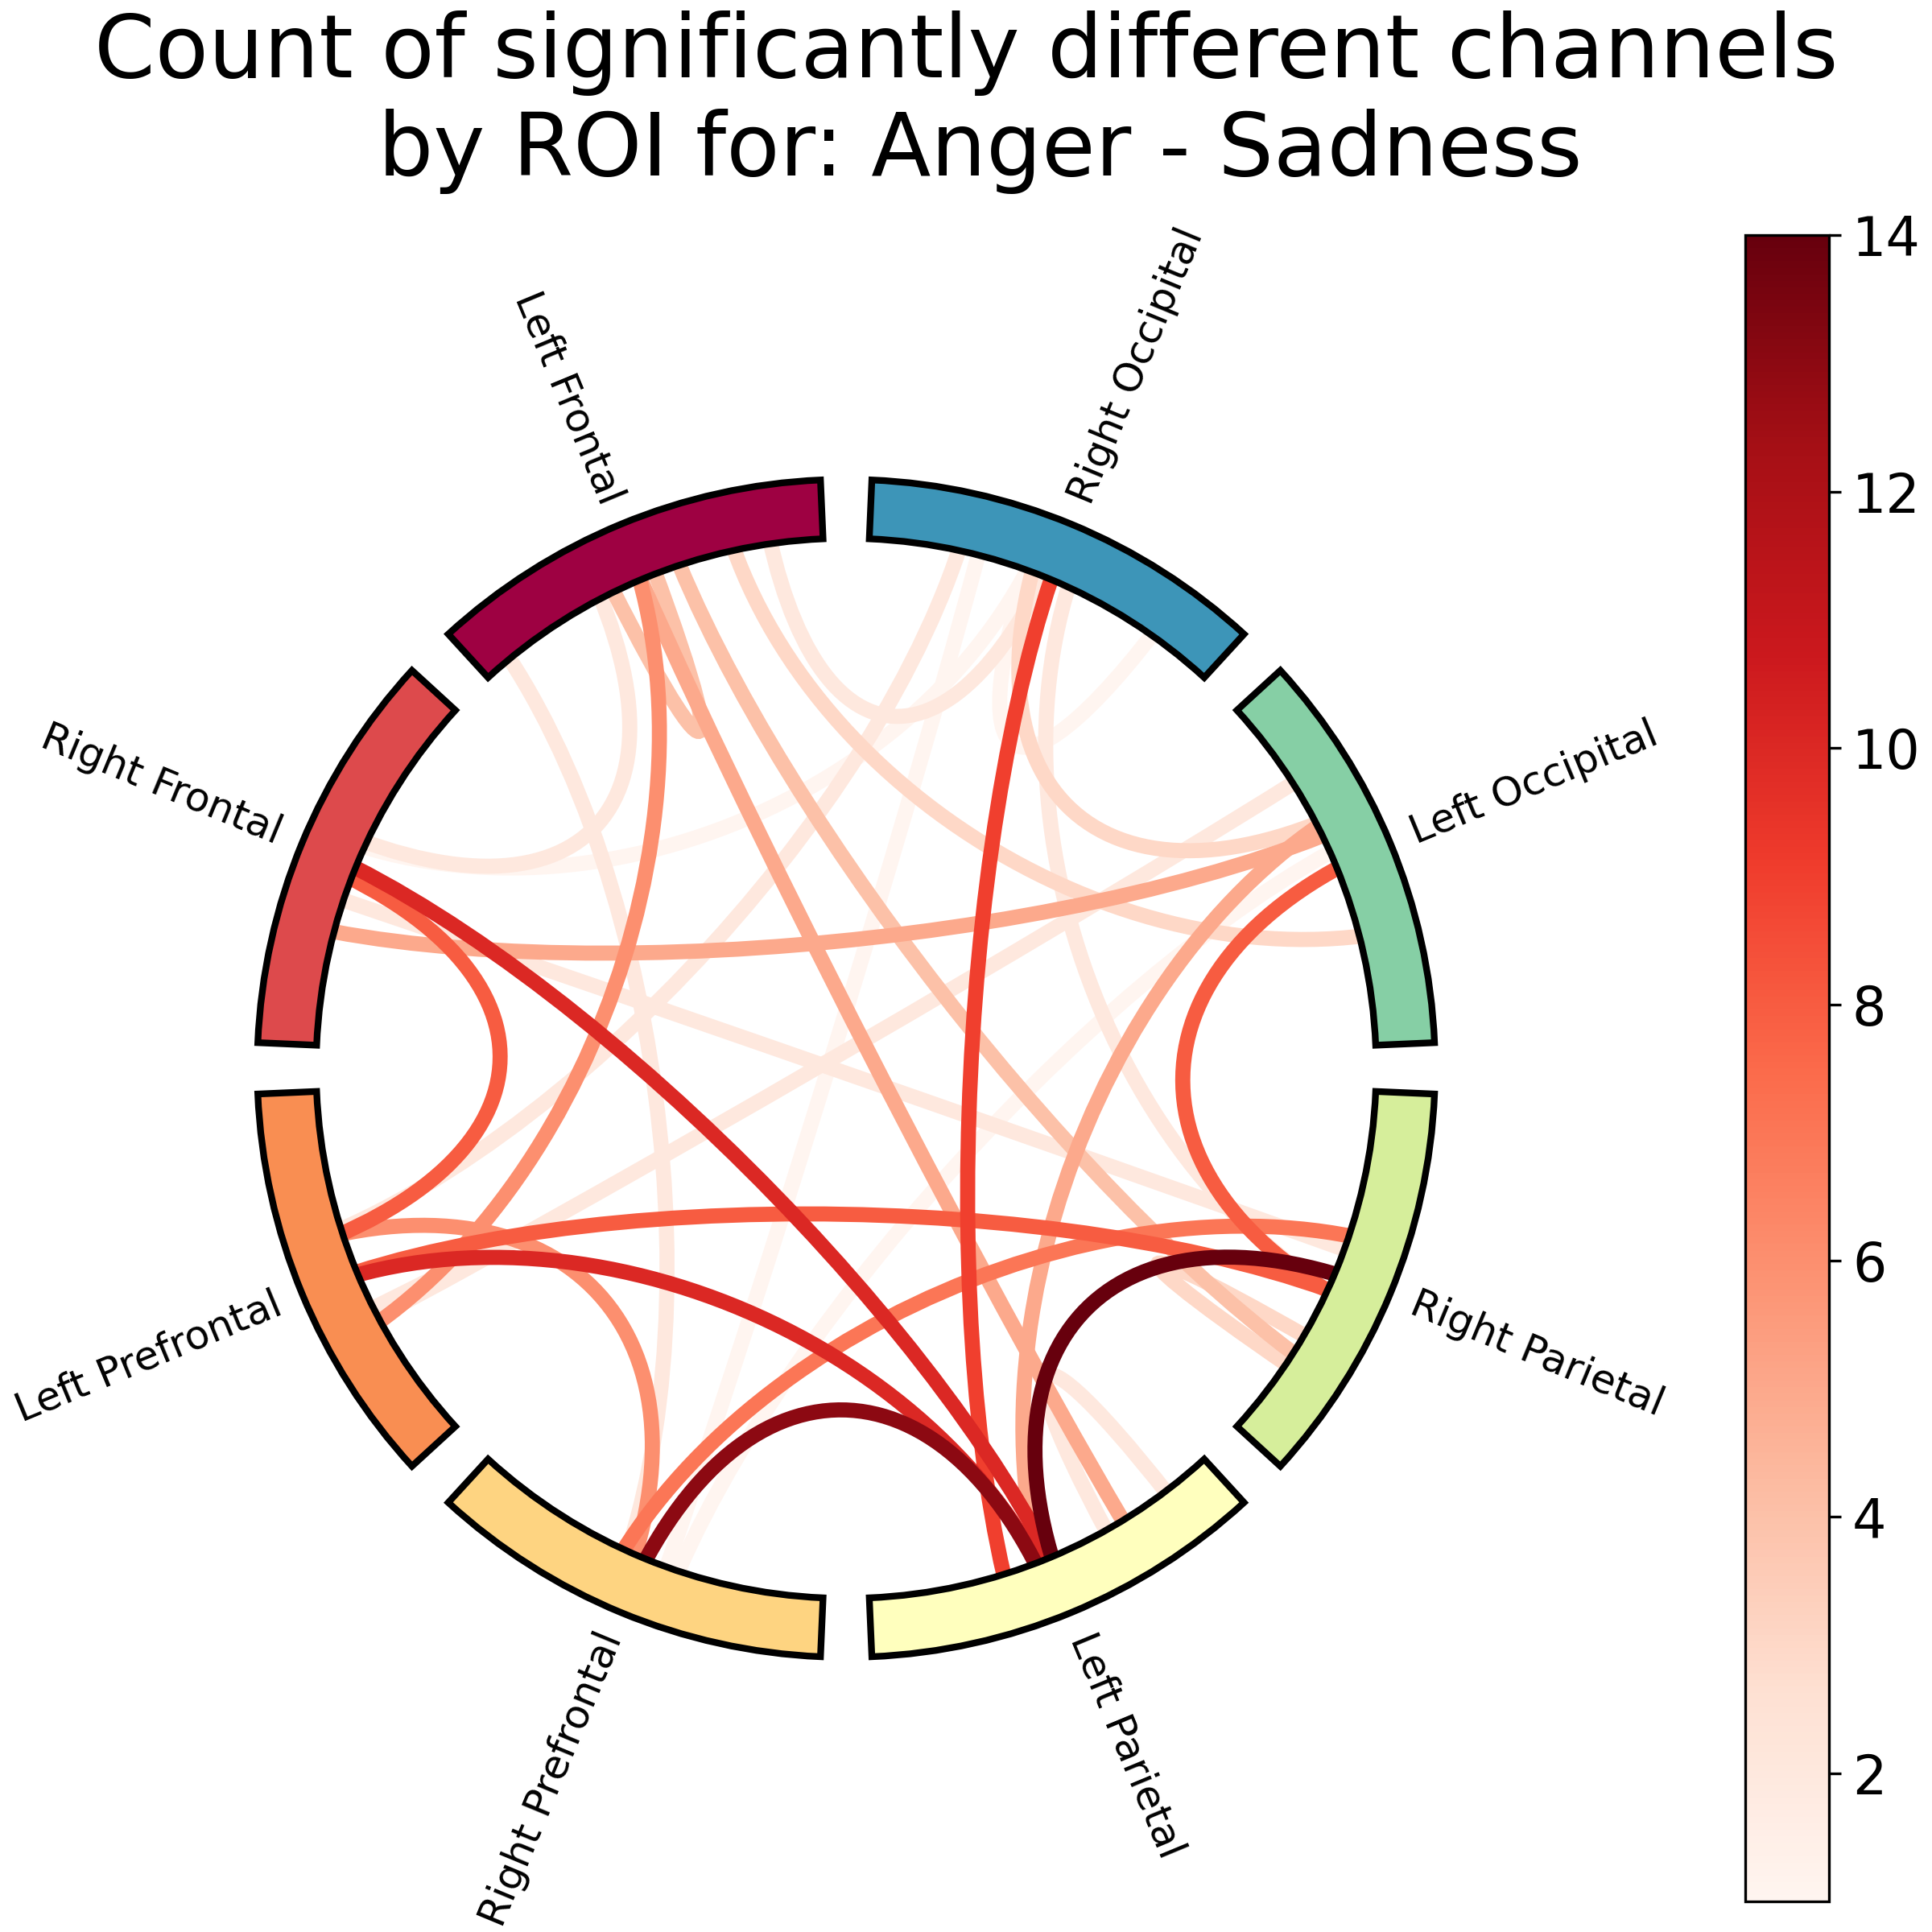
\includegraphics[width=0.24\textwidth]{C:/Users/super/OneDrive - Ontario Tech University/fNIRS_Emotions/plots/spectral_connectivity_time/chord_plots/group_level_t_tests_roi/emotion_Anger_Sadness.png}
  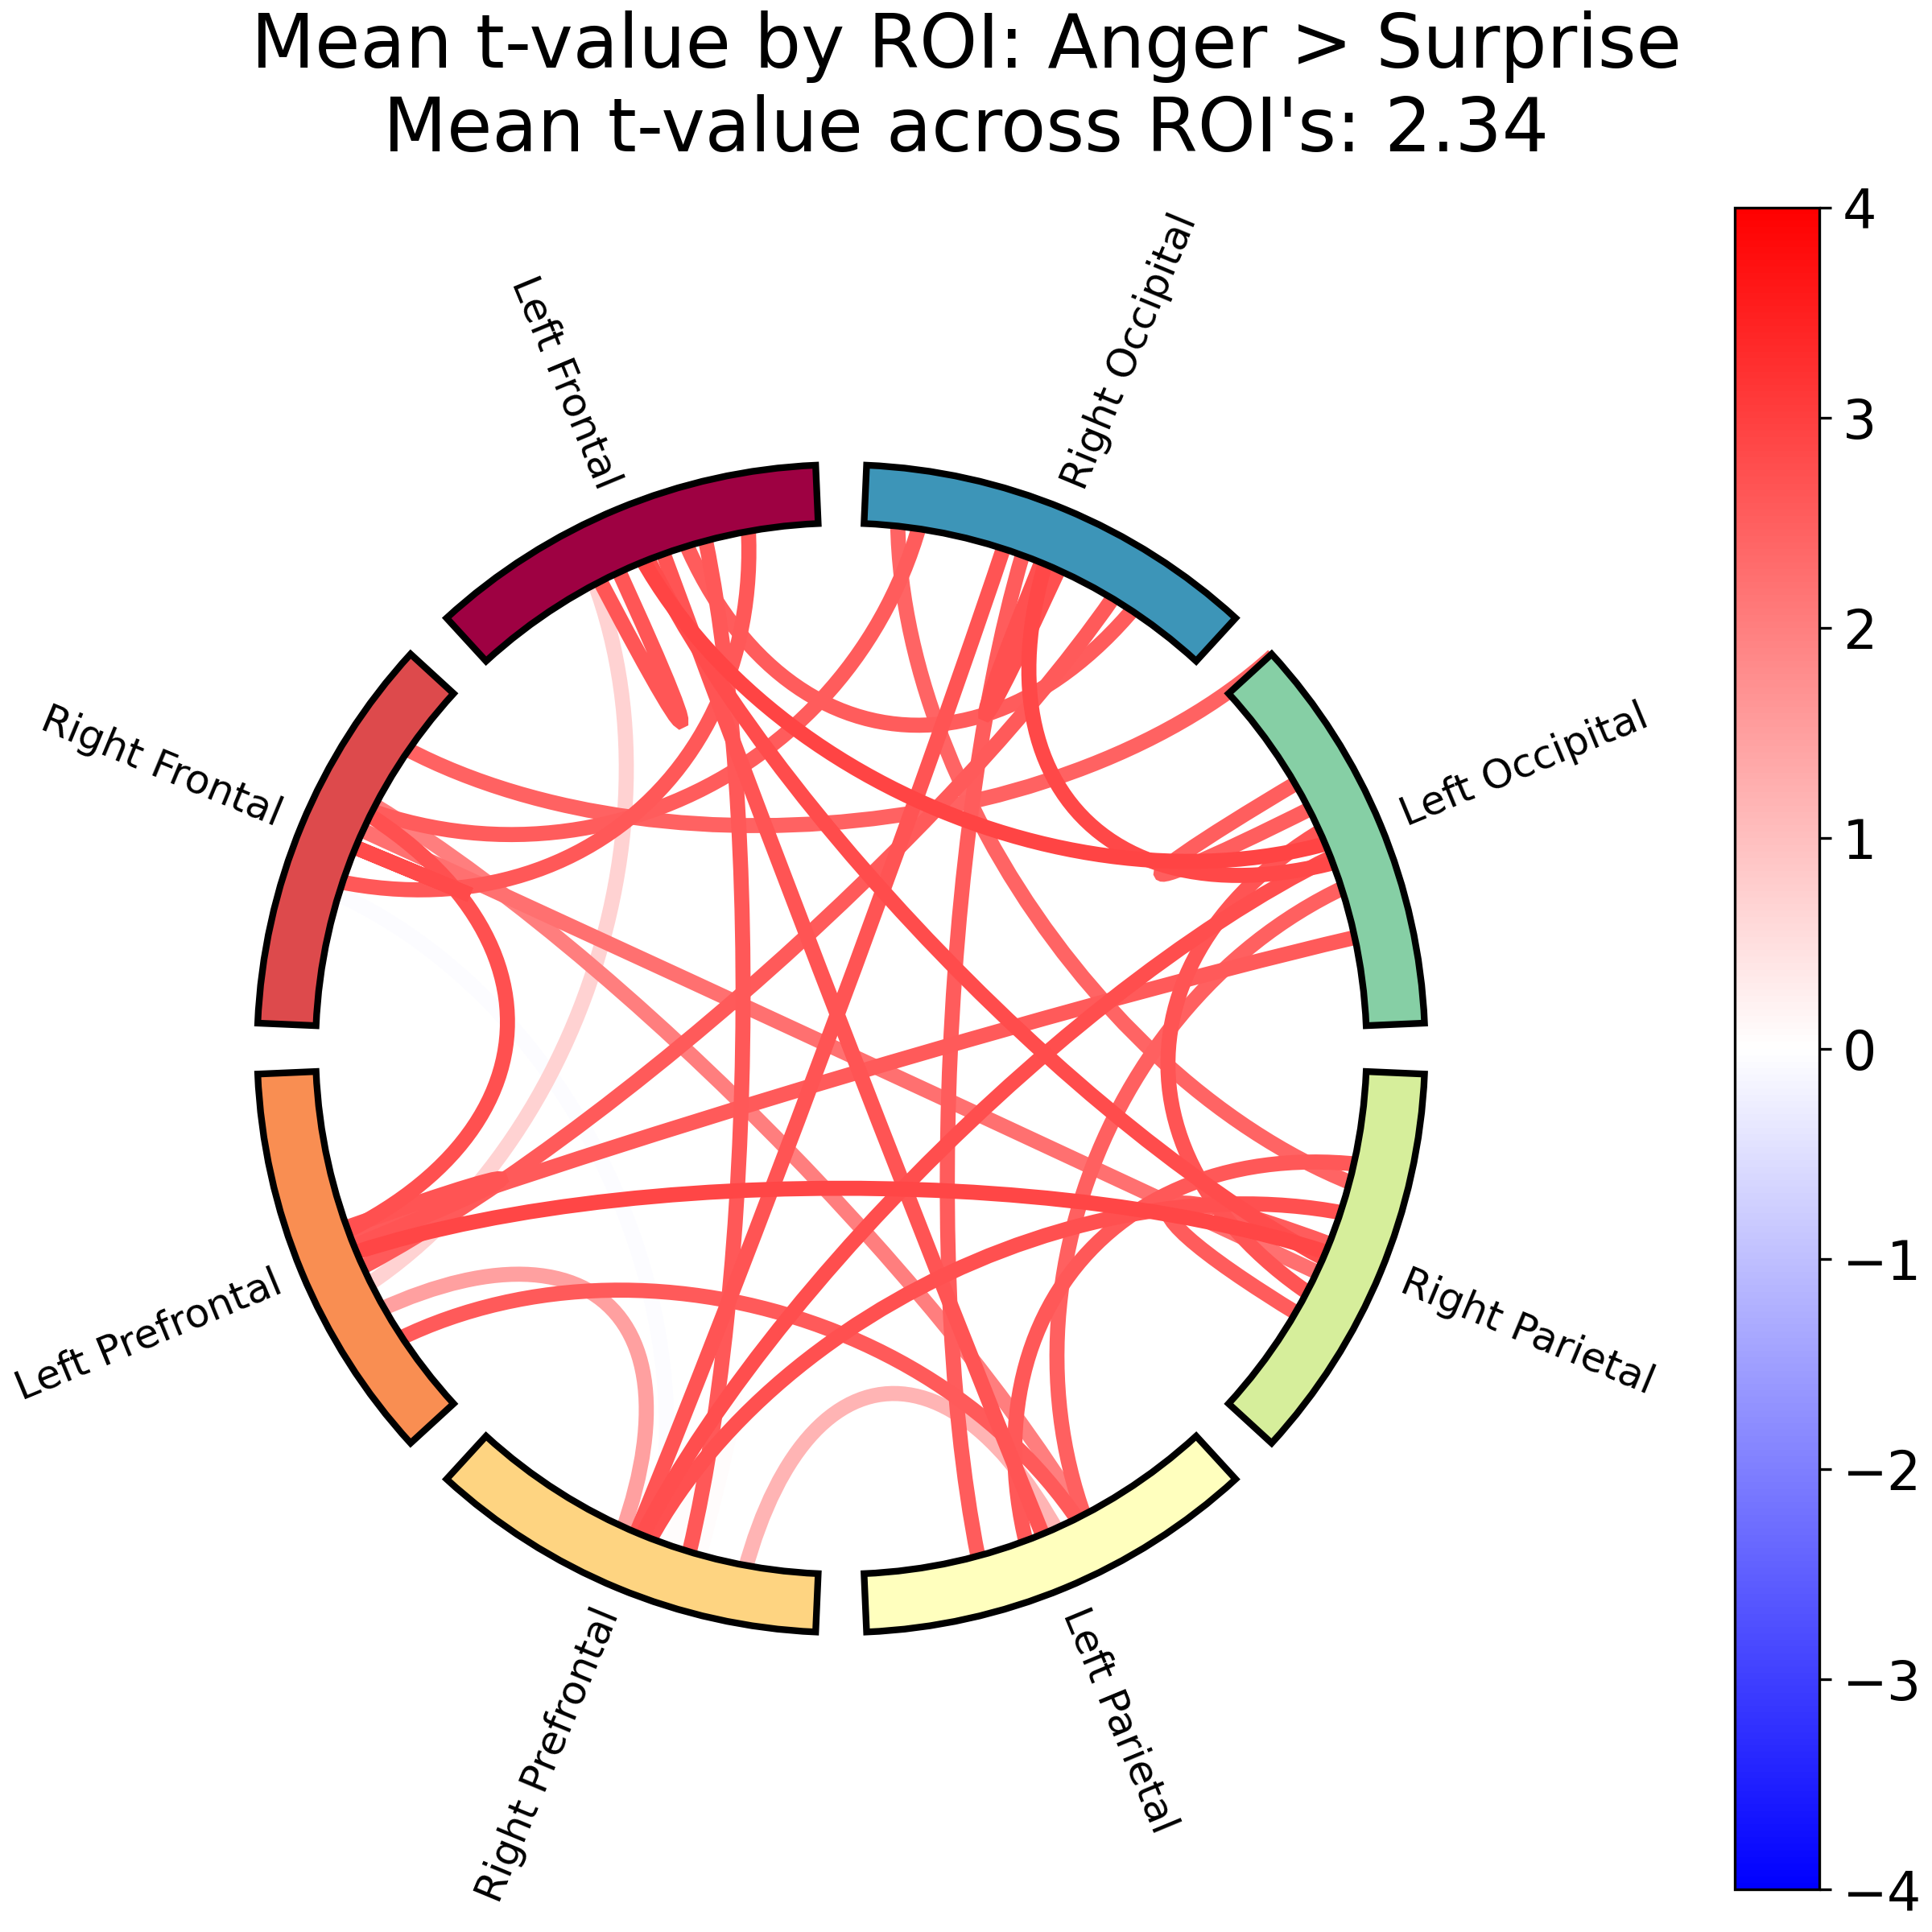
\includegraphics[width=0.24\textwidth]{C:/Users/super/OneDrive - Ontario Tech University/fNIRS_Emotions/plots/spectral_connectivity_time/chord_plots/group_level_t_tests_roi/emotion_Anger_Surprise.png}
  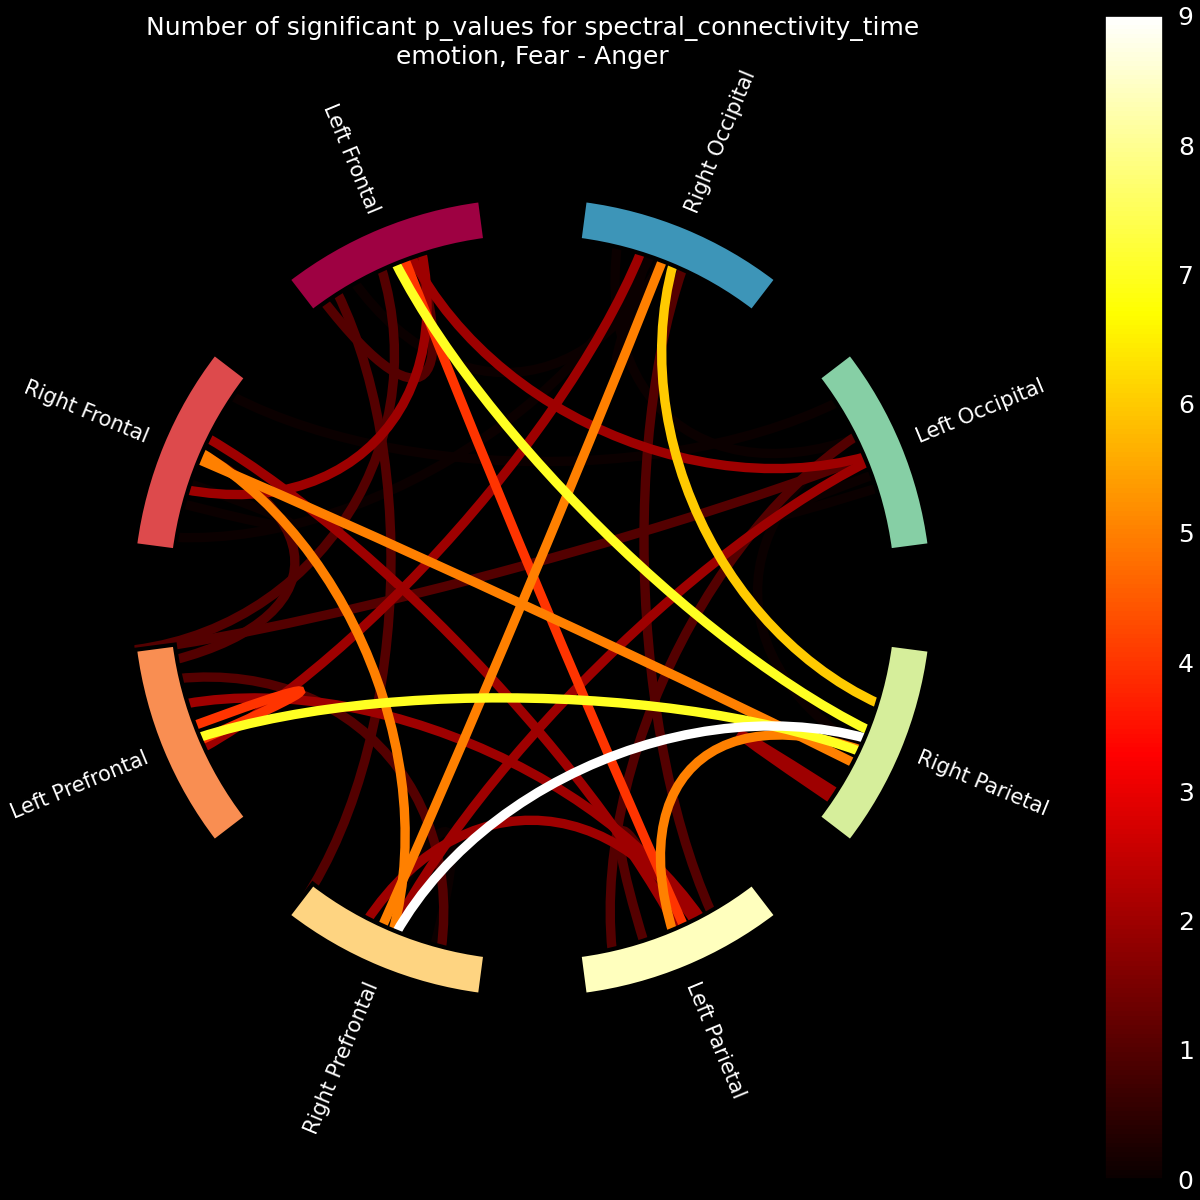
\includegraphics[width=0.24\textwidth]{C:/Users/super/OneDrive - Ontario Tech University/fNIRS_Emotions/plots/spectral_connectivity_time/chord_plots/group_level_t_tests_roi/emotion_Fear_Anger.png}
  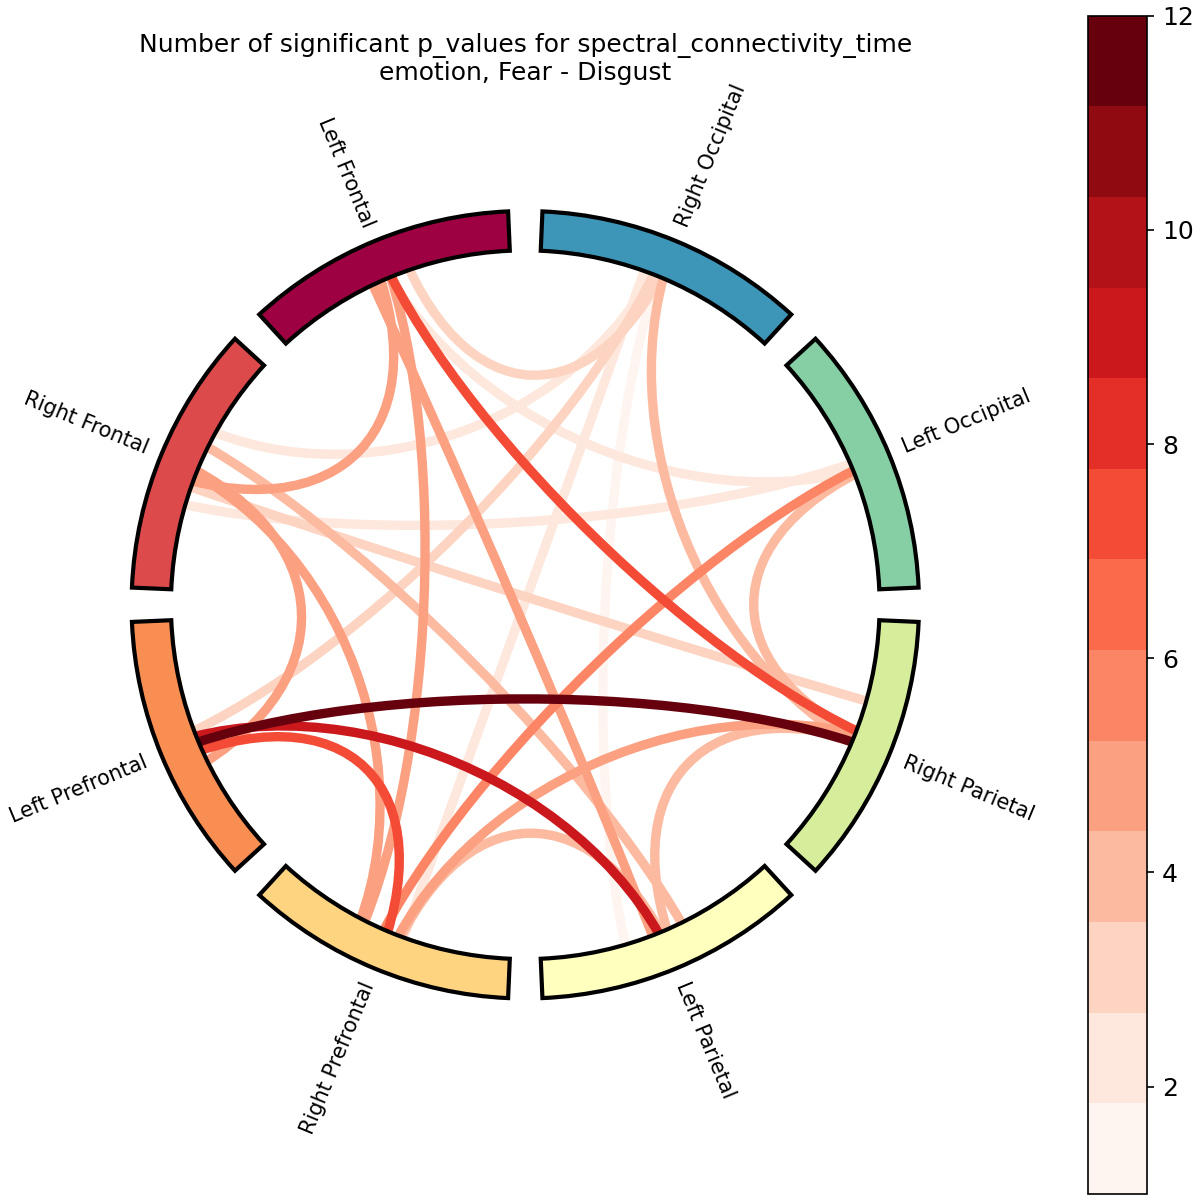
\includegraphics[width=0.24\textwidth]{C:/Users/super/OneDrive - Ontario Tech University/fNIRS_Emotions/plots/spectral_connectivity_time/chord_plots/group_level_t_tests_roi/emotion_Fear_Disgust.png}
  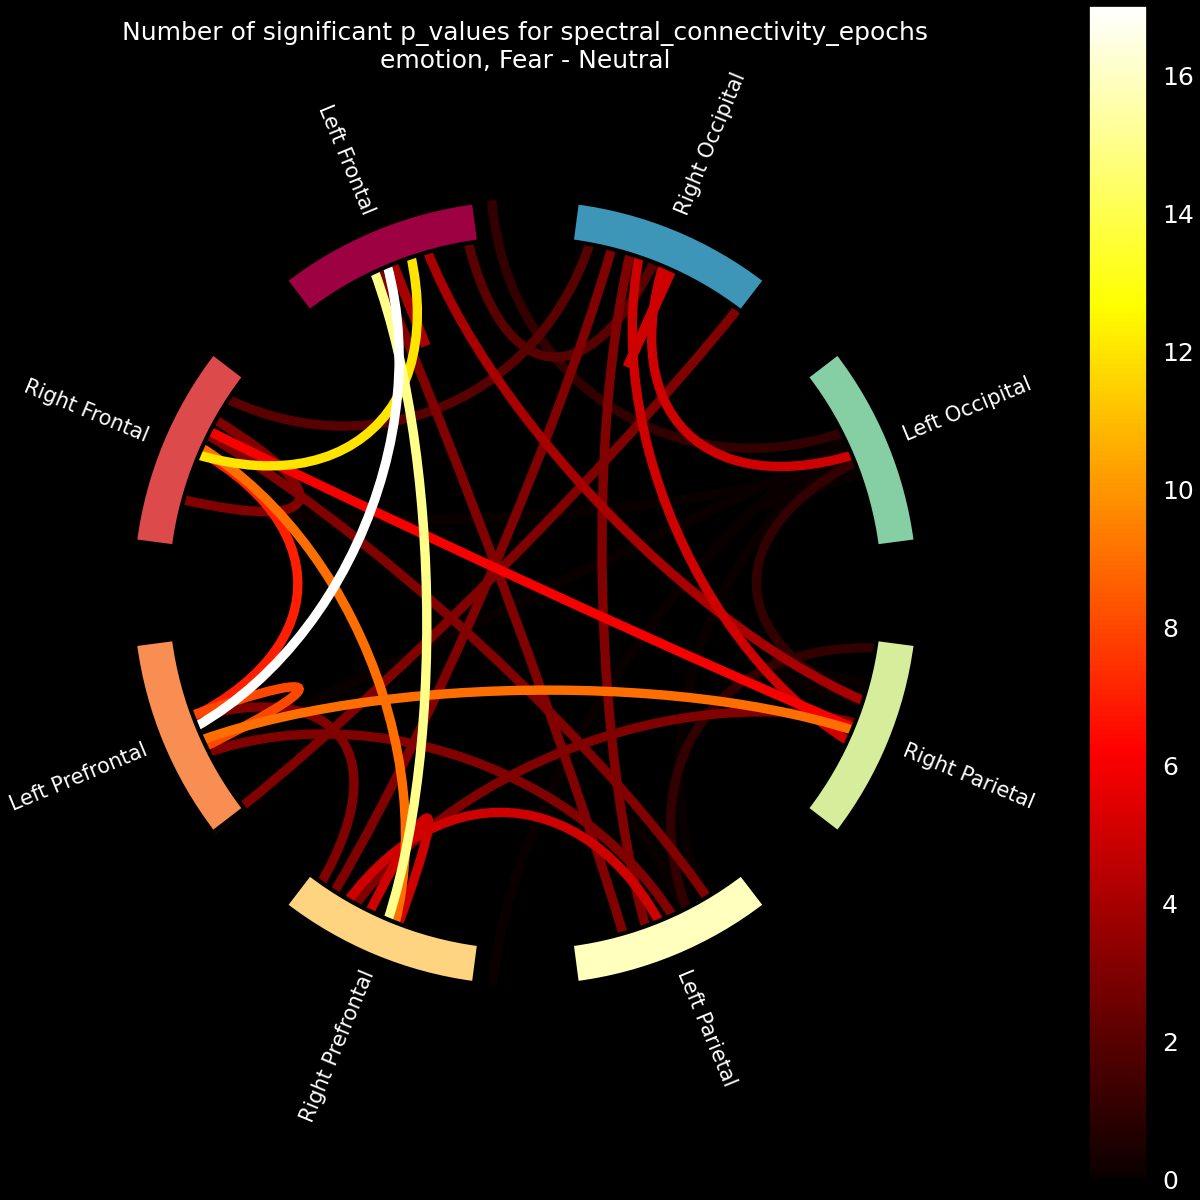
\includegraphics[width=0.24\textwidth]{C:/Users/super/OneDrive - Ontario Tech University/fNIRS_Emotions/plots/spectral_connectivity_time/chord_plots/group_level_t_tests_roi/emotion_Fear_Neutral.png}
  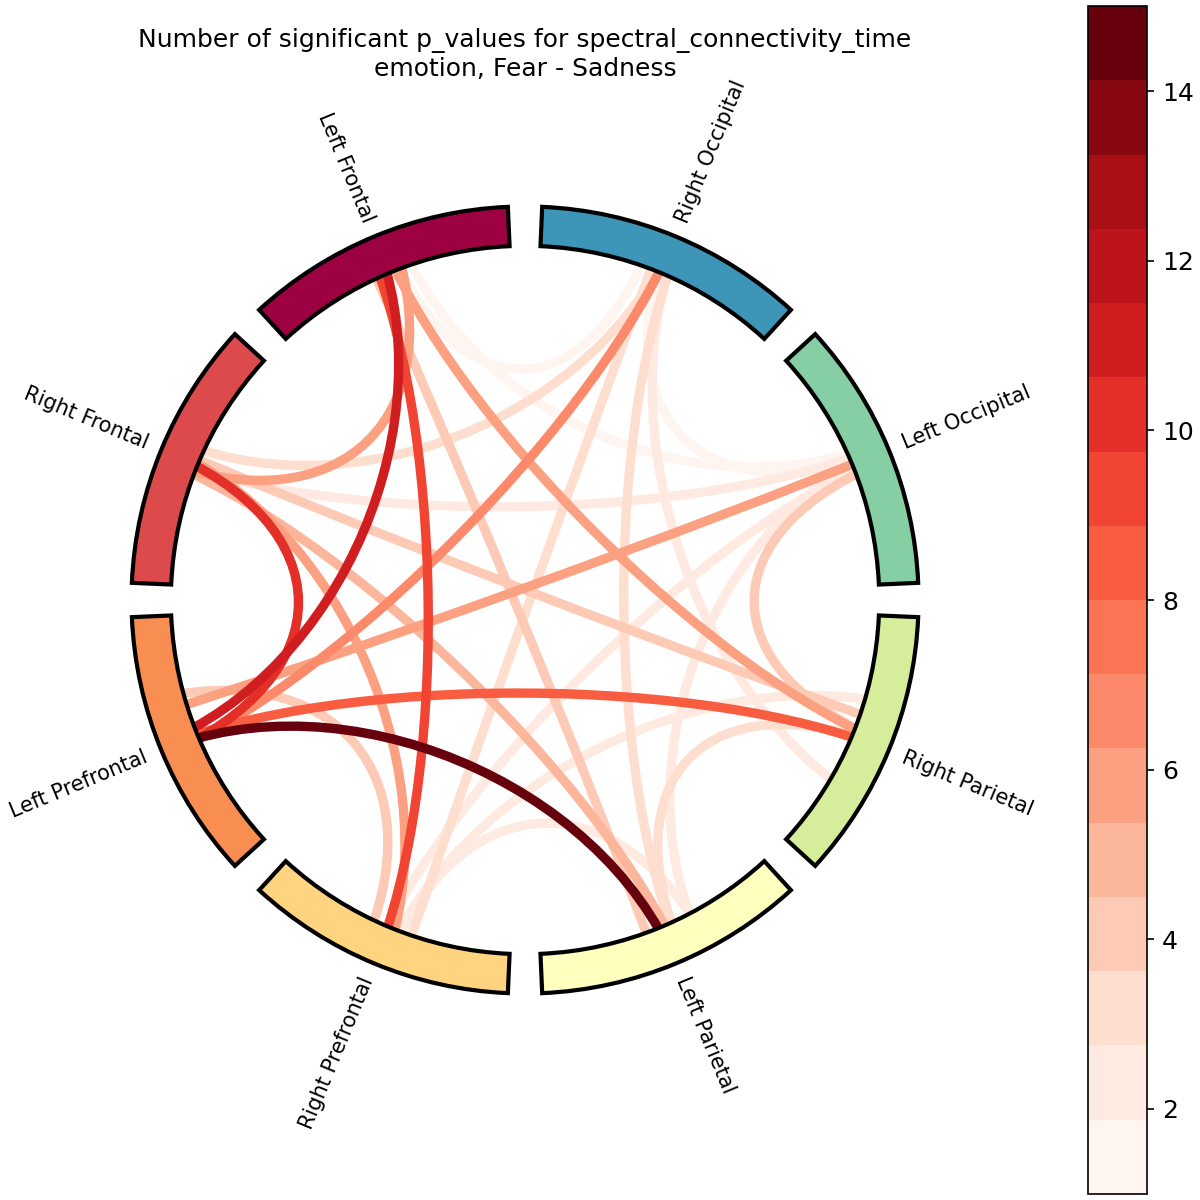
\includegraphics[width=0.24\textwidth]{C:/Users/super/OneDrive - Ontario Tech University/fNIRS_Emotions/plots/spectral_connectivity_time/chord_plots/group_level_t_tests_roi/emotion_Fear_Sadness.png}
  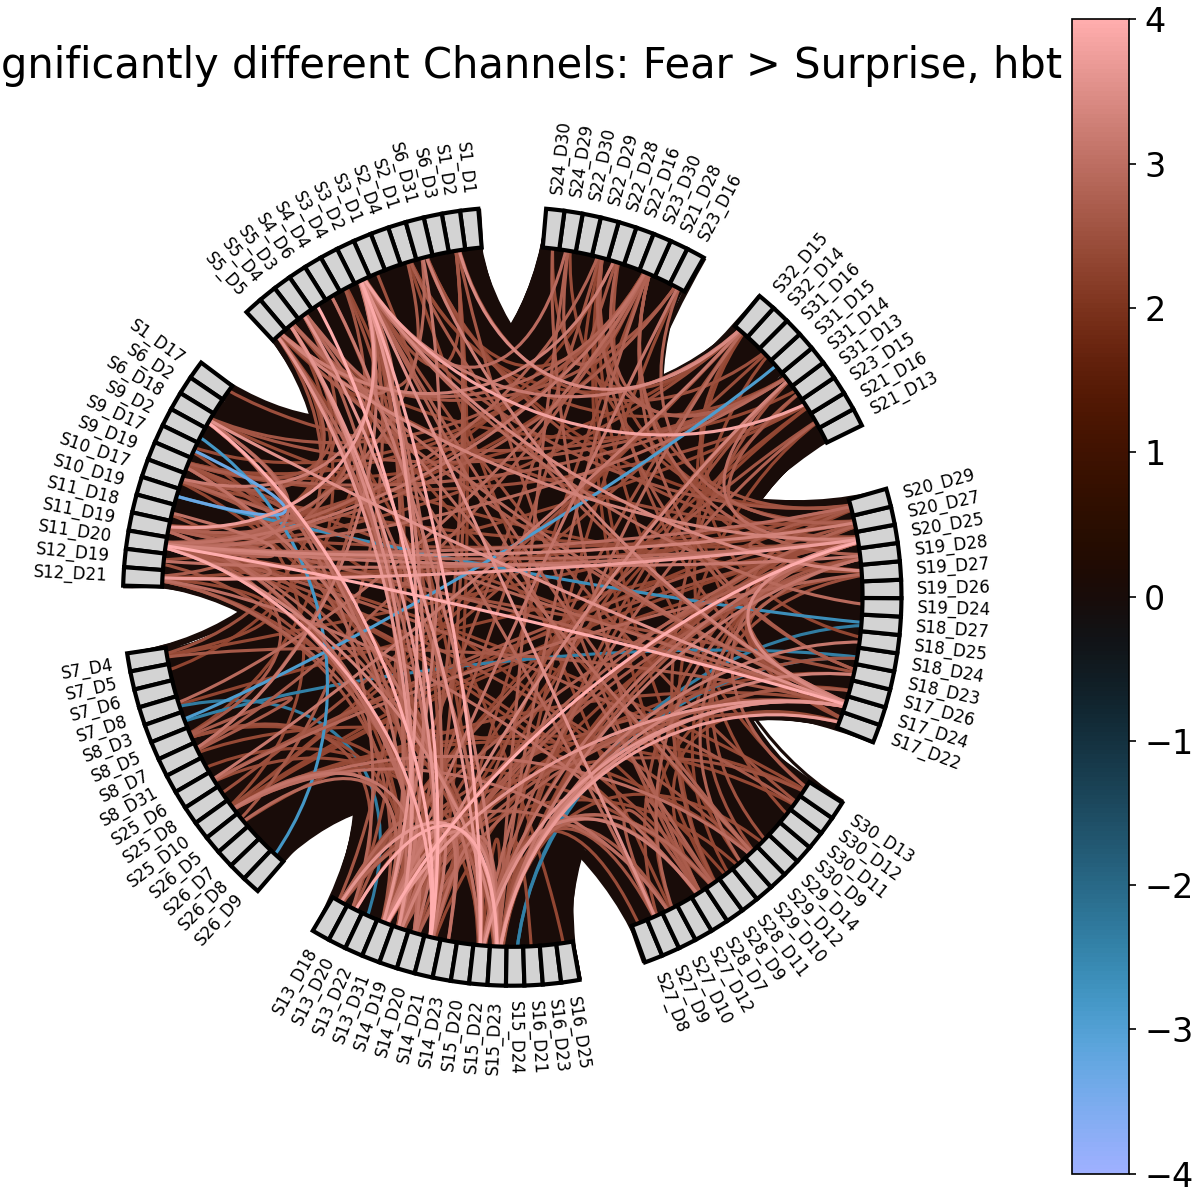
\includegraphics[width=0.24\textwidth]{C:/Users/super/OneDrive - Ontario Tech University/fNIRS_Emotions/plots/spectral_connectivity_time/chord_plots/group_level_t_tests_roi/emotion_Fear_Surprise.png}
  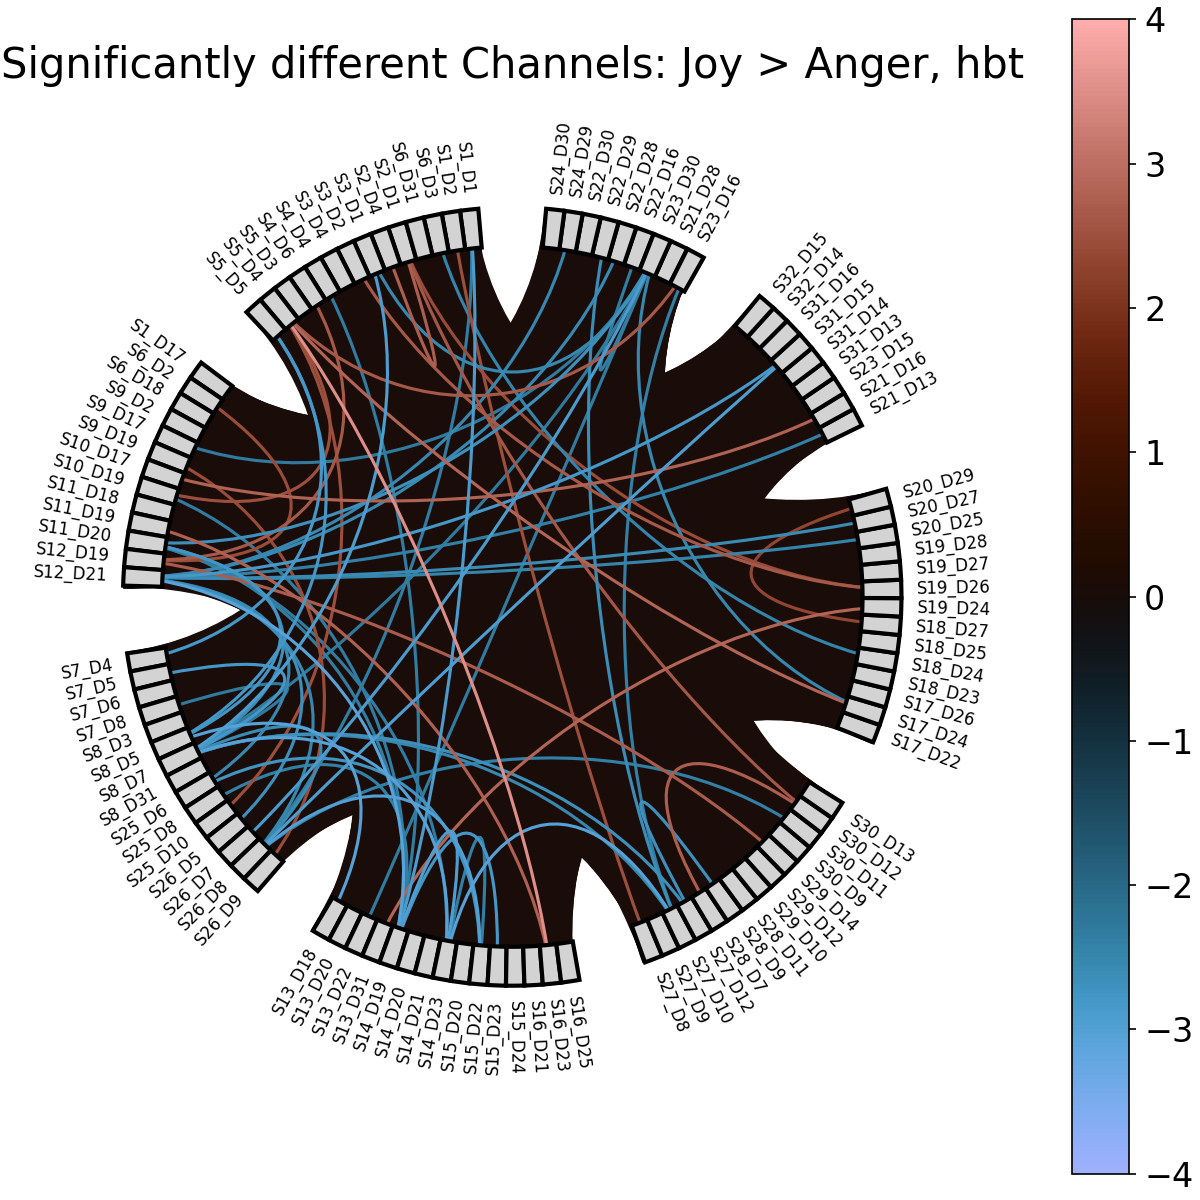
\includegraphics[width=0.24\textwidth]{C:/Users/super/OneDrive - Ontario Tech University/fNIRS_Emotions/plots/spectral_connectivity_time/chord_plots/group_level_t_tests_roi/emotion_Joy_Anger.png}
  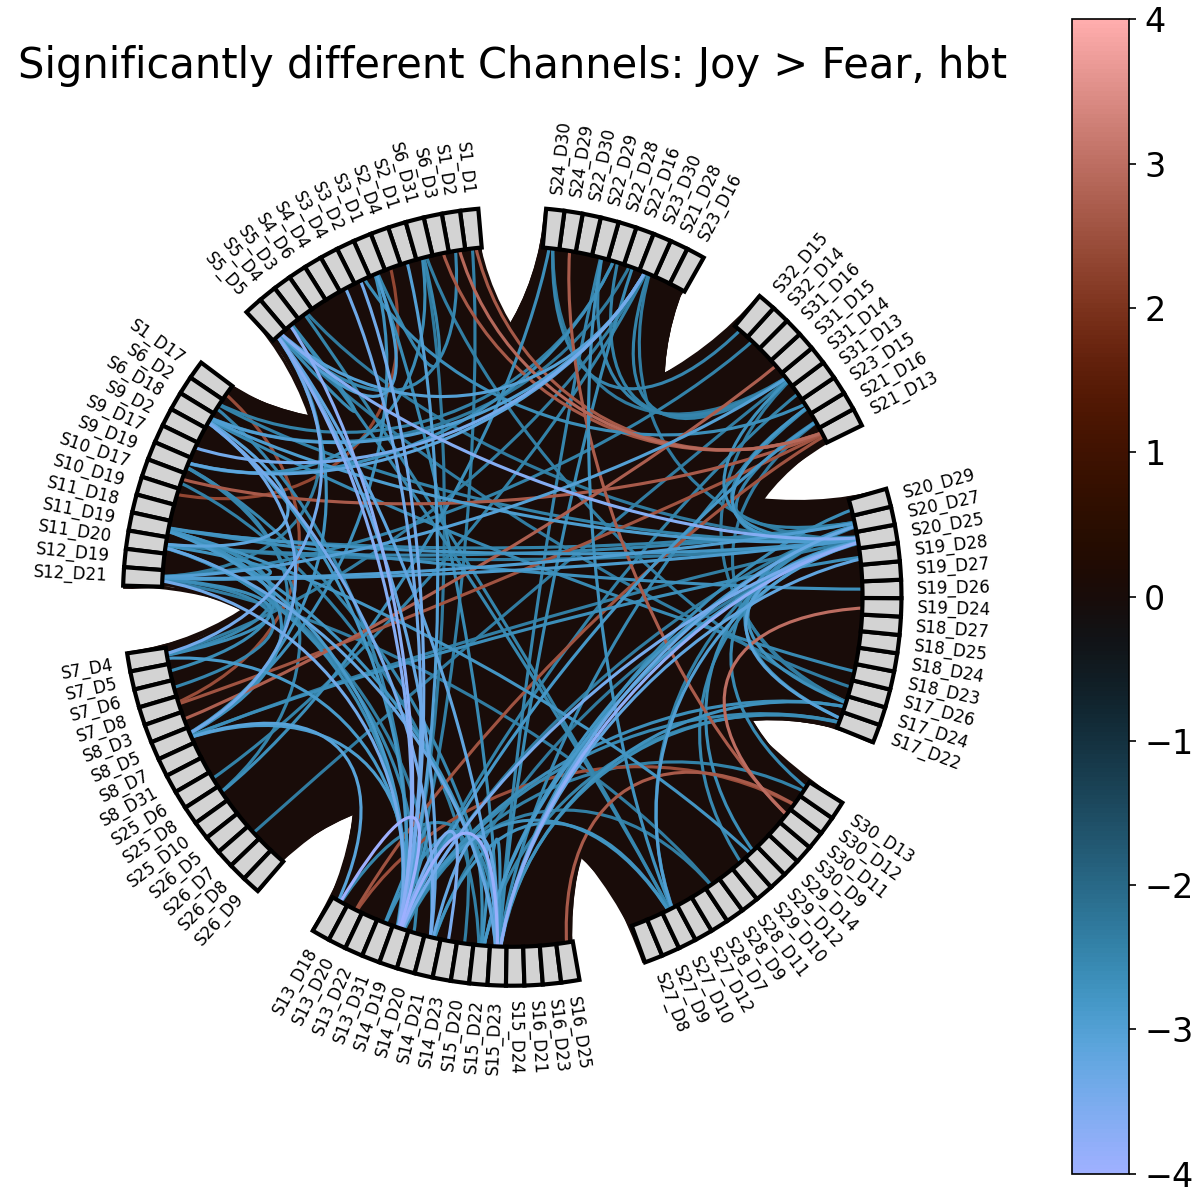
\includegraphics[width=0.24\textwidth]{C:/Users/super/OneDrive - Ontario Tech University/fNIRS_Emotions/plots/spectral_connectivity_time/chord_plots/group_level_t_tests_roi/emotion_Joy_Fear.png}
  \caption[FC: Emotion Contrasts (Fear and Anger)]{Functional connectivity results for Fear and Anger vs. the other emotions.
  Same concept as explained in figure \ref{fig:fc_real_vs_virtual}. }
  \label{fig:fc_emotion_analysis}
\end{figure}

The emotion contrasts (as shown in \ref{fig:fc_emotion_analysis}) revealed significant differences in functional connectivity across different emotions and ROI's.
The $t$-values show that Anger and Fear showed higher connectivity in general compared to the other emotions, and when compared to each other, Fear has only slightly higher connectivity than Anger. 
This higher connectivity for Anger and Fear as compared to the other emotions is consistent across most ROI's as well. 
The rest of the emotion contrasts can be found in Appendix \ref{tab:appendix_fc_emotion_analysis}, which shows the remaining set of contrasts for all emotions.

\begin{figure}[H]
  \centering
  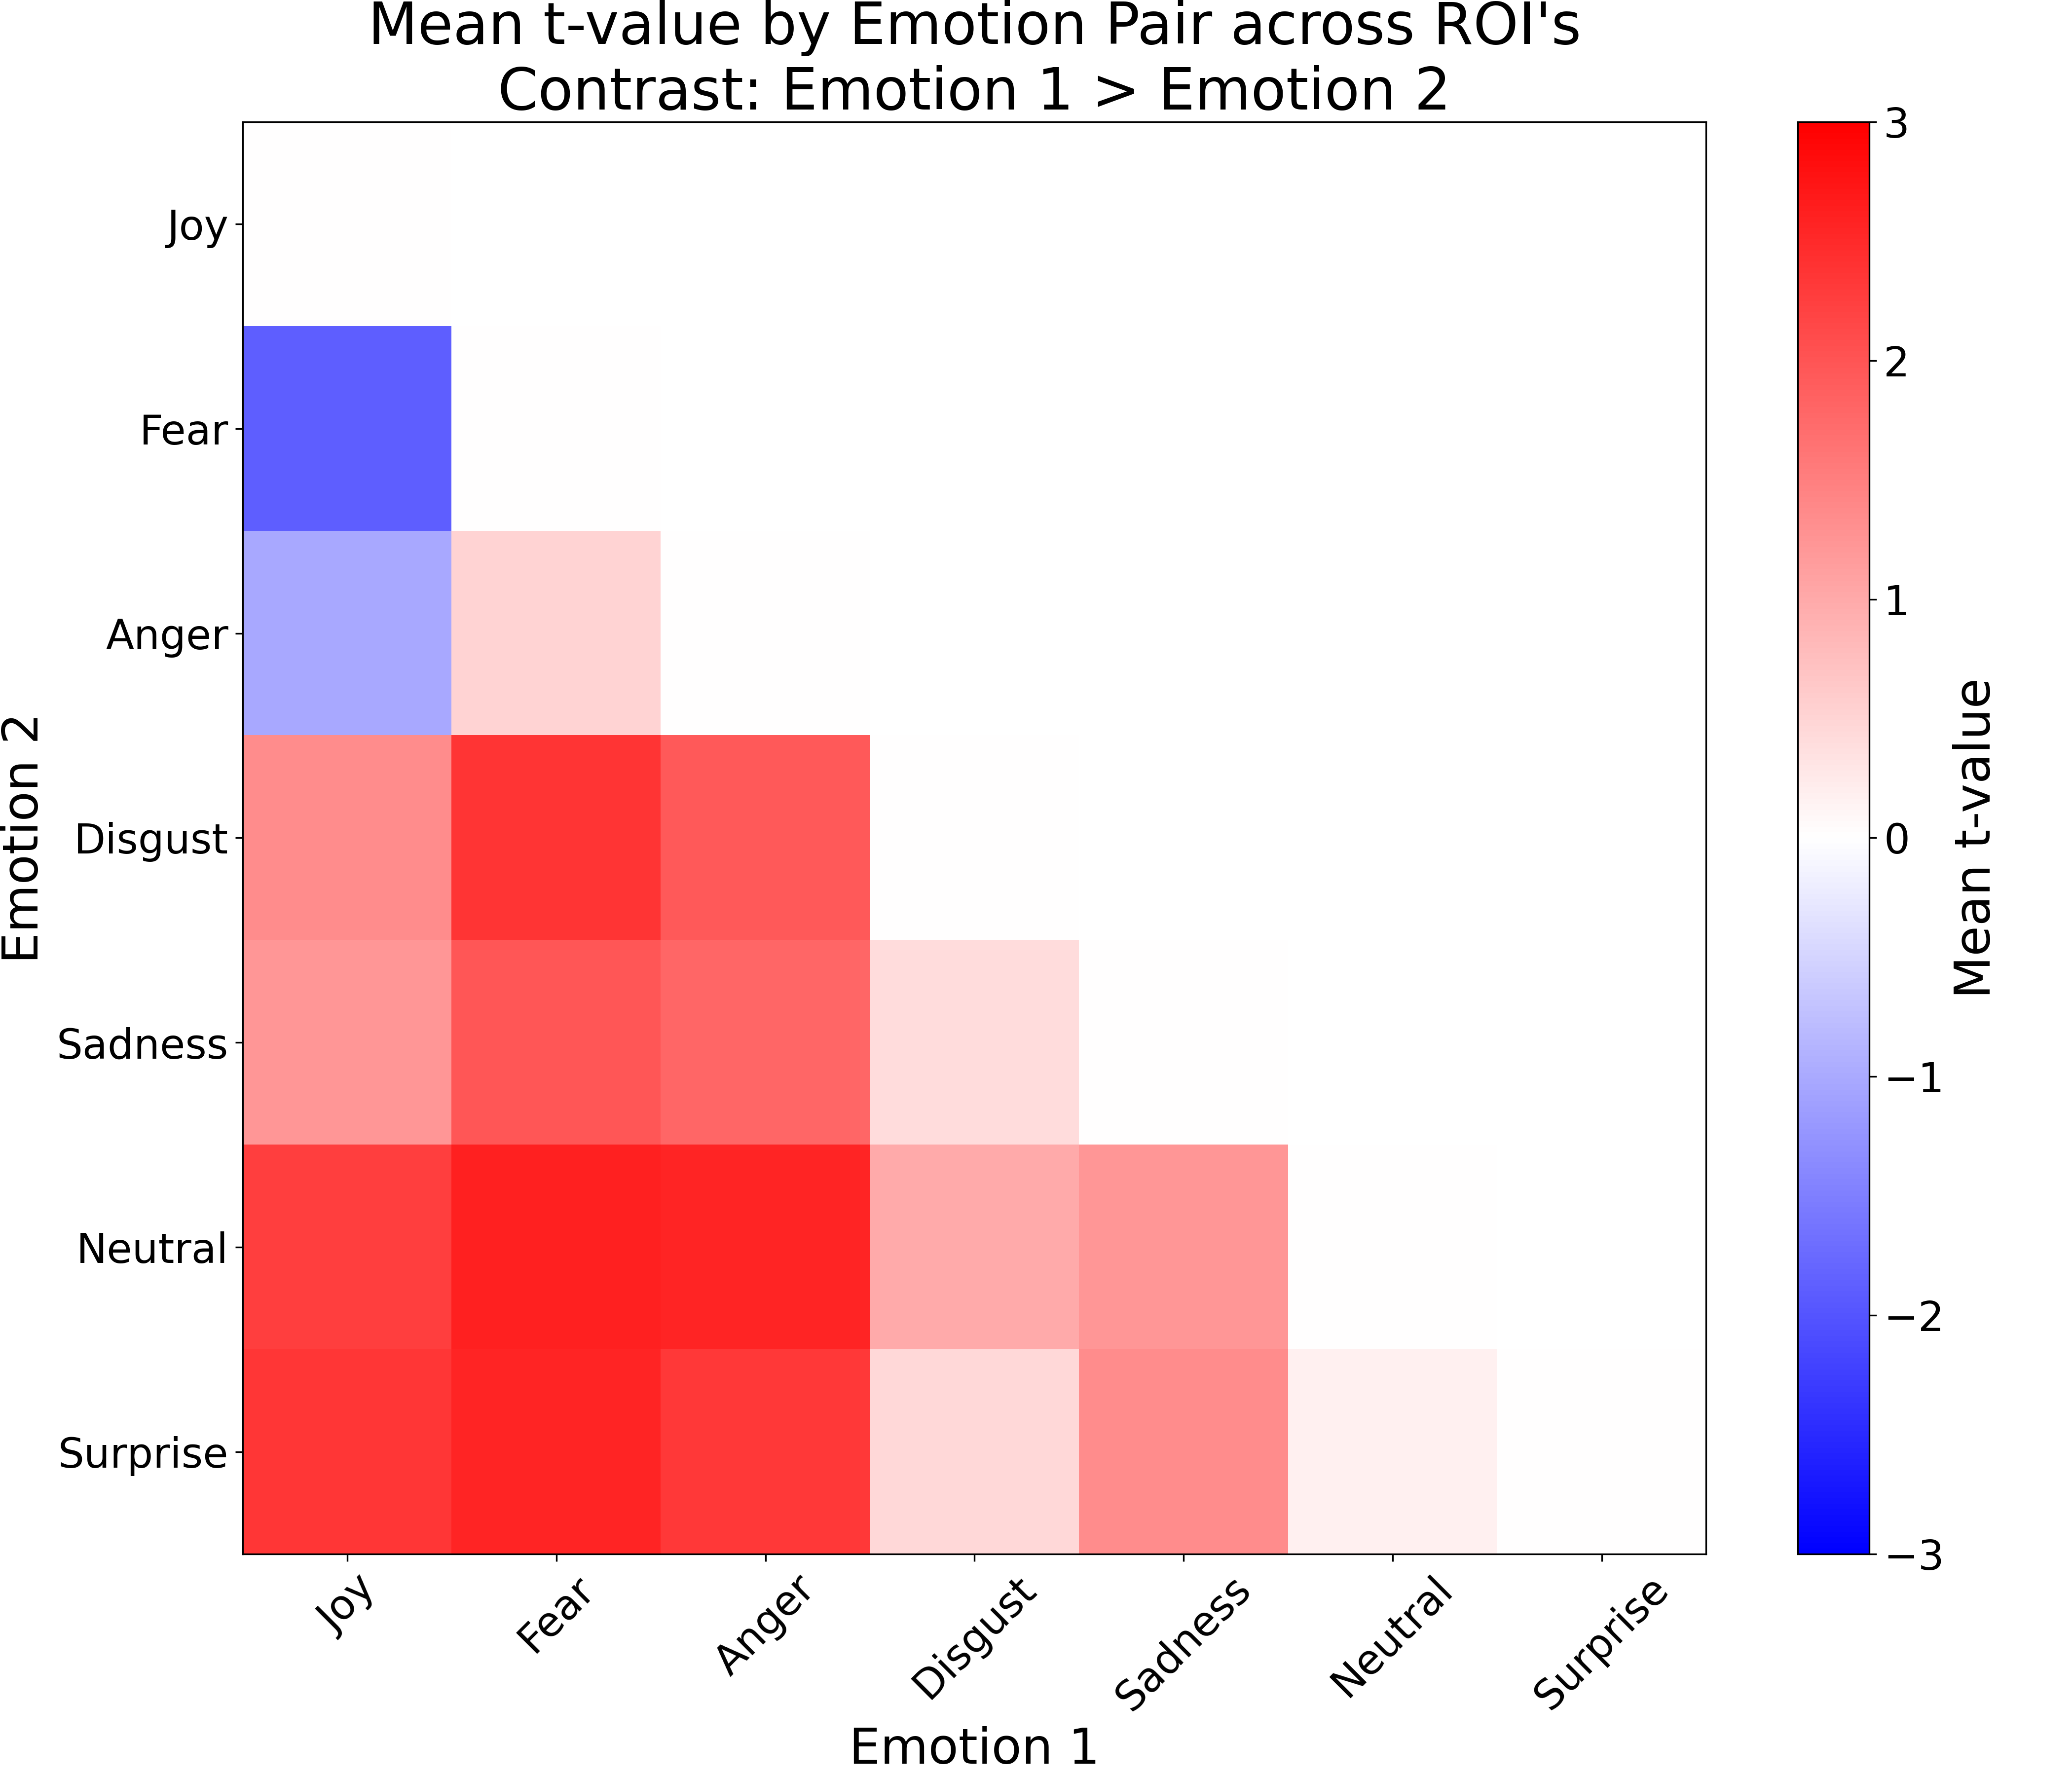
\includegraphics[width=1\textwidth]{C:/Users/super/OneDrive - Ontario Tech University/fNIRS_Emotions/plots/spectral_connectivity_time/emotion_analysis/Mean_t-value_by_Emotion_Pair.png}
  \caption[FC: Summary of Contrasts by Emotion Pair]{A heatmap summary of the functional connectivity results for the contrasts between different emotions.
  Red signifies that emotion 1 has higher connectivity than emotion 2, while blue signifies that emotion 2 has higher connectivity than emotion 1.
  The color bar on the right shows the $t$-value averaged across all significant channel pairs and across all ROI's, which indicates the strength of the difference in connectivity between the two emotions.
  This is the same value that is shown at the top of each plot in figure \ref{fig:fc_real_vs_virtual} and \ref{fig:fc_emotion_analysis}.}
  \label{fig:fc_emotion_summary_analysis}
\end{figure}

This summary of the functional connectivity results for the contrasts between different emotions (as shown in \ref{fig:fc_emotion_summary_analysis}) shows that Anger and Fear have the highest connectivity compared to the other emotions, with Fear having slightly higher connectivity than Anger.
This lines up with figure \ref{fig:fc_emotion_analysis}, which shows that Anger and Fear have higher connectivity compared to the other emotions.

\begin{figure}[H]
  \centering
  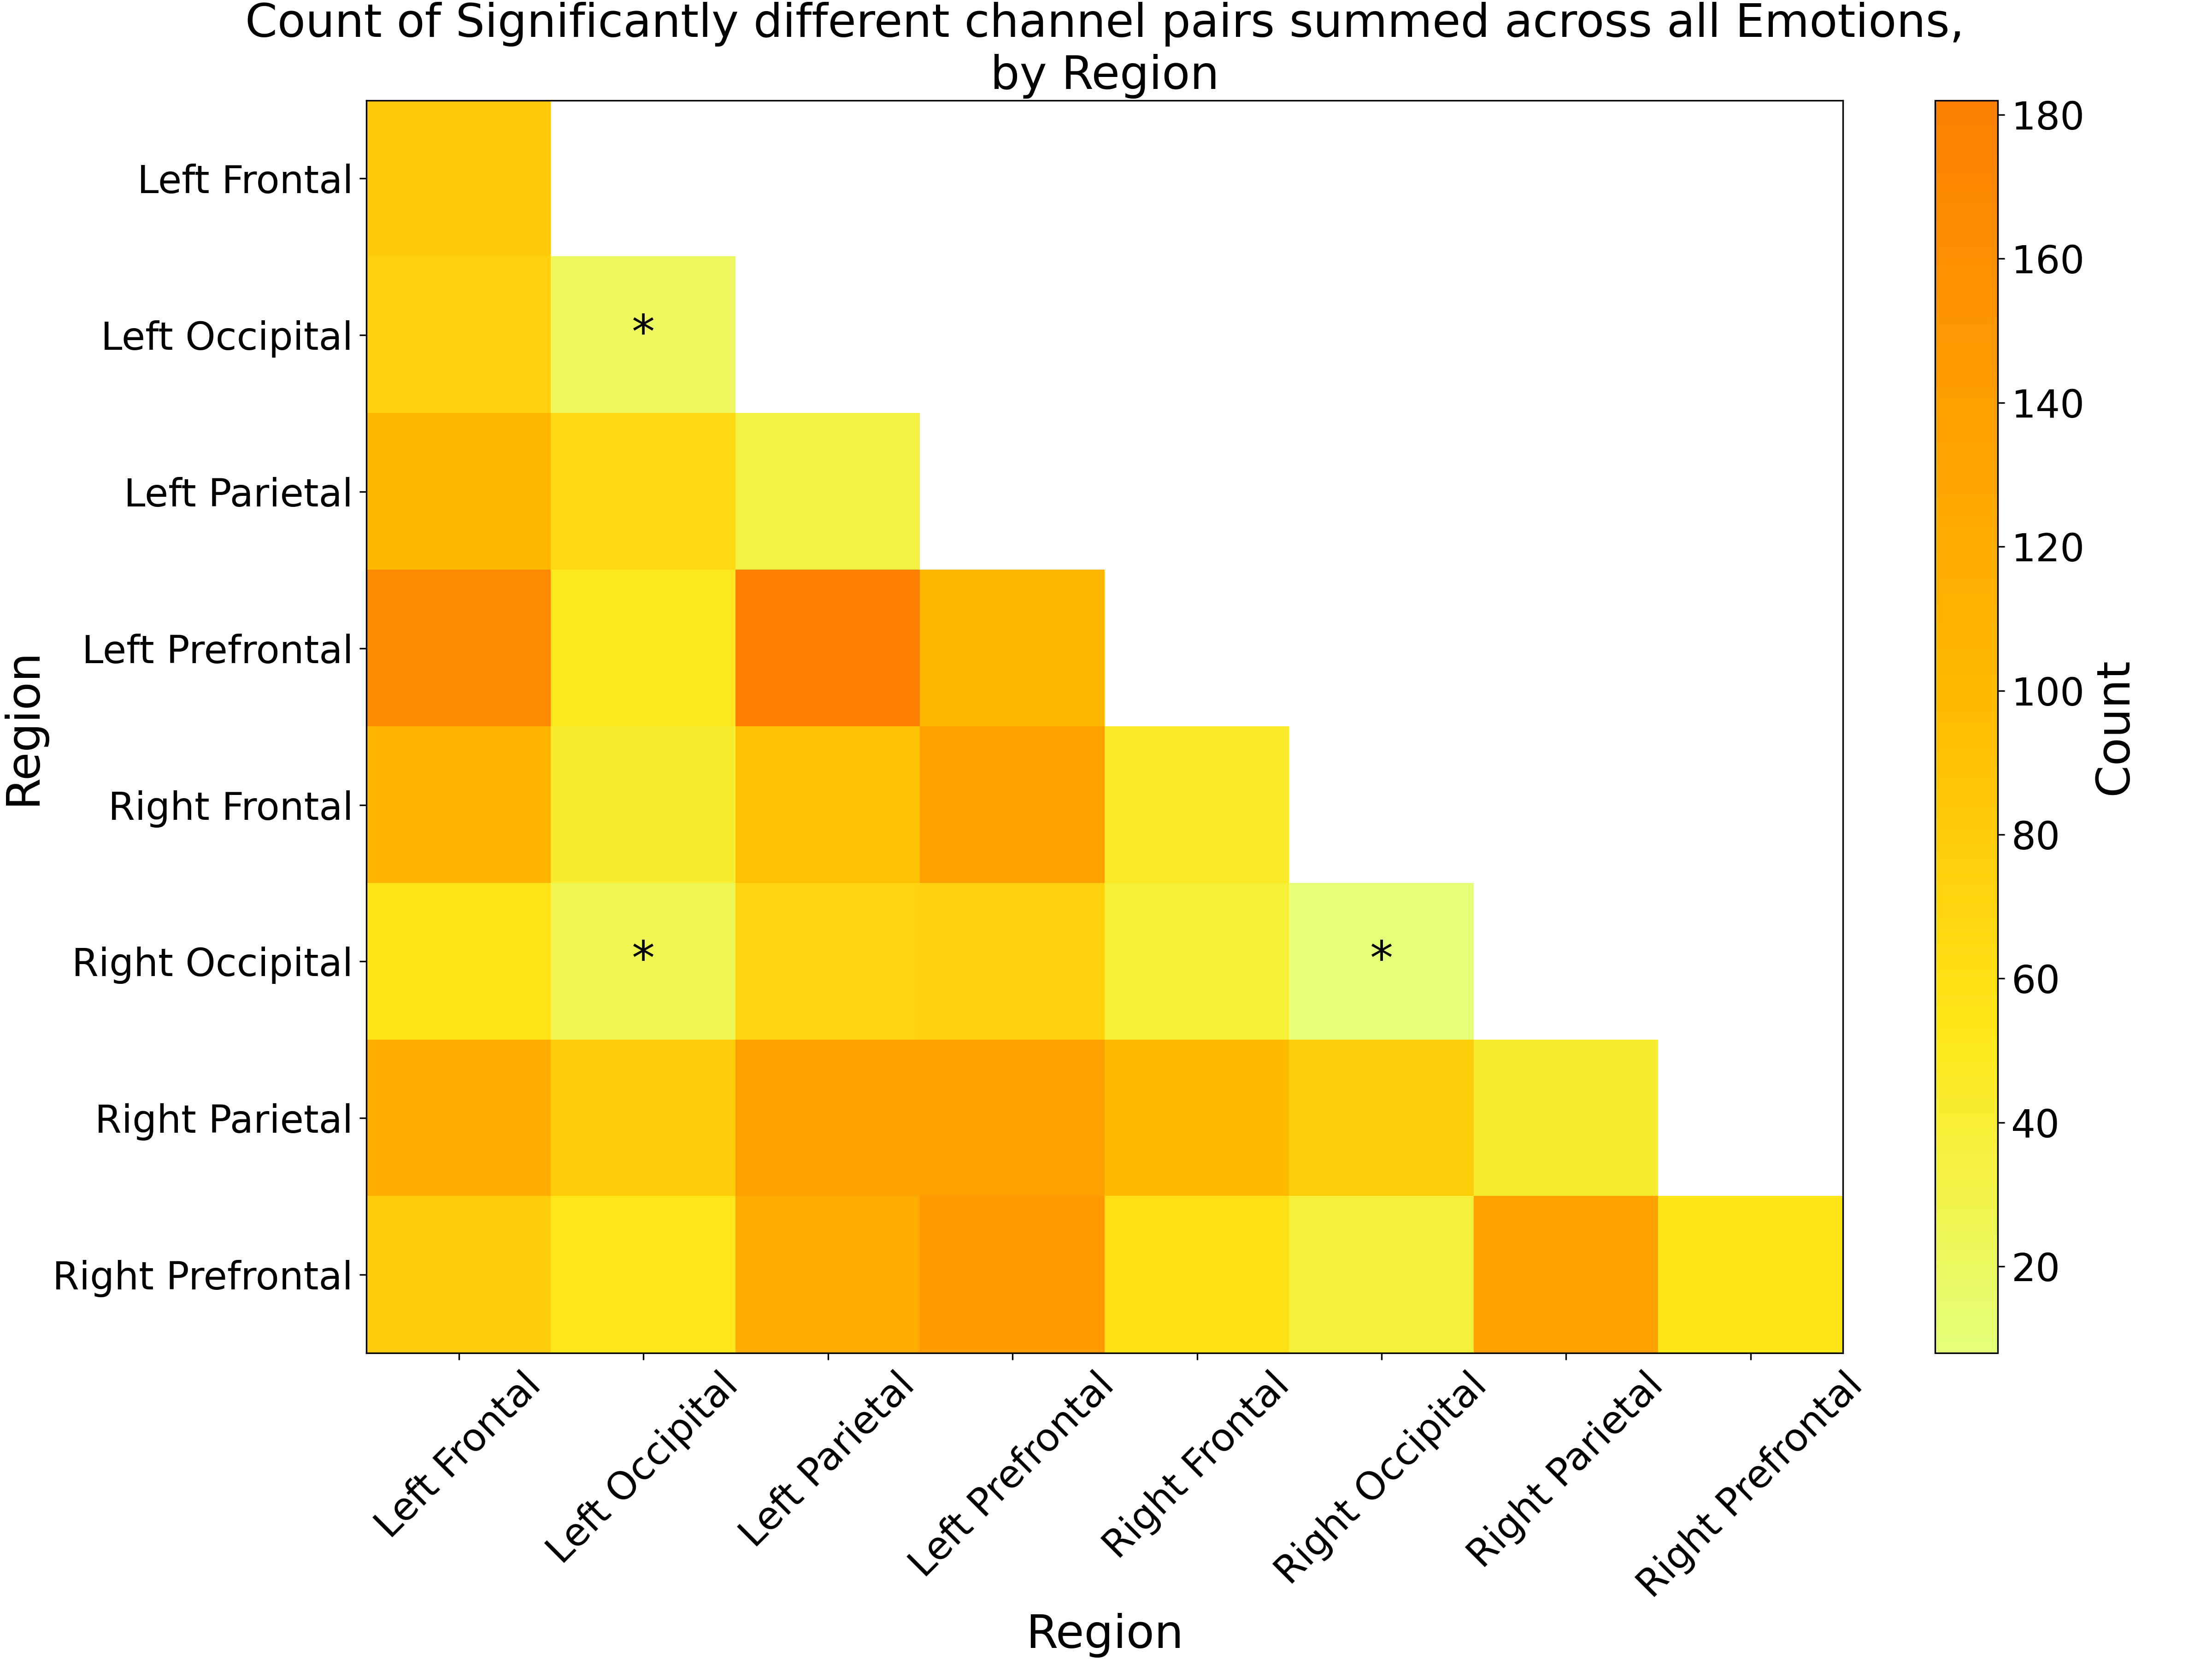
\includegraphics[width=1\textwidth]{C:/Users/super/OneDrive - Ontario Tech University/fNIRS_Emotions/plots/spectral_connectivity_time/emotion_analysis/Count_of_Significant_Channel_Pairs_by_Region.png}
  \caption[FC: Count of Significantly Different Channel Pairs by ROI]{A heatmap summary of the number of significantly different channel pairs for each ROI summed across all emotions. 
  The color bar on the right shows the number of significant channel pairs for each ROI, with brighter colors indicating a smaller number of significant channel pairs, and darker colors indicating a larger number of significant channel pairs.
  An asterisk was placed on the 3 ROI's with the least number of significantly different channel pairs to indicate that these ROI's are more synchronized with each other than any other pair of ROI's, regardless of the emotion.
  Note that ROI's can have differences within them, as each ROI is made up of multiple channels, and the differences are calculated between channels within the same ROI.}
  \label{fig:fc_region_summary_analysis}
\end{figure}

The count of significantly different channel pairs for each ROI summed across all emotions (as shown in \ref{fig:fc_region_summary_analysis}) marks 3 regions with an asterisk, these regions have less channel pairs that are significantly different from each other, meaning that these regions are more synchronized with each other than any other pair of ROI's.
These regions are the left occipital/right occipital, left occipital/left occipital, and right occipital/right occipital ROI's.
This indicates that the differences in processing emotions occur in the frontal, prefrontal, and parietal regions of the brain.

\subsection{Face Type \texorpdfstring{$\times$}{x} Emotion Contrasts}
\begin{figure}[H]
  \centering
  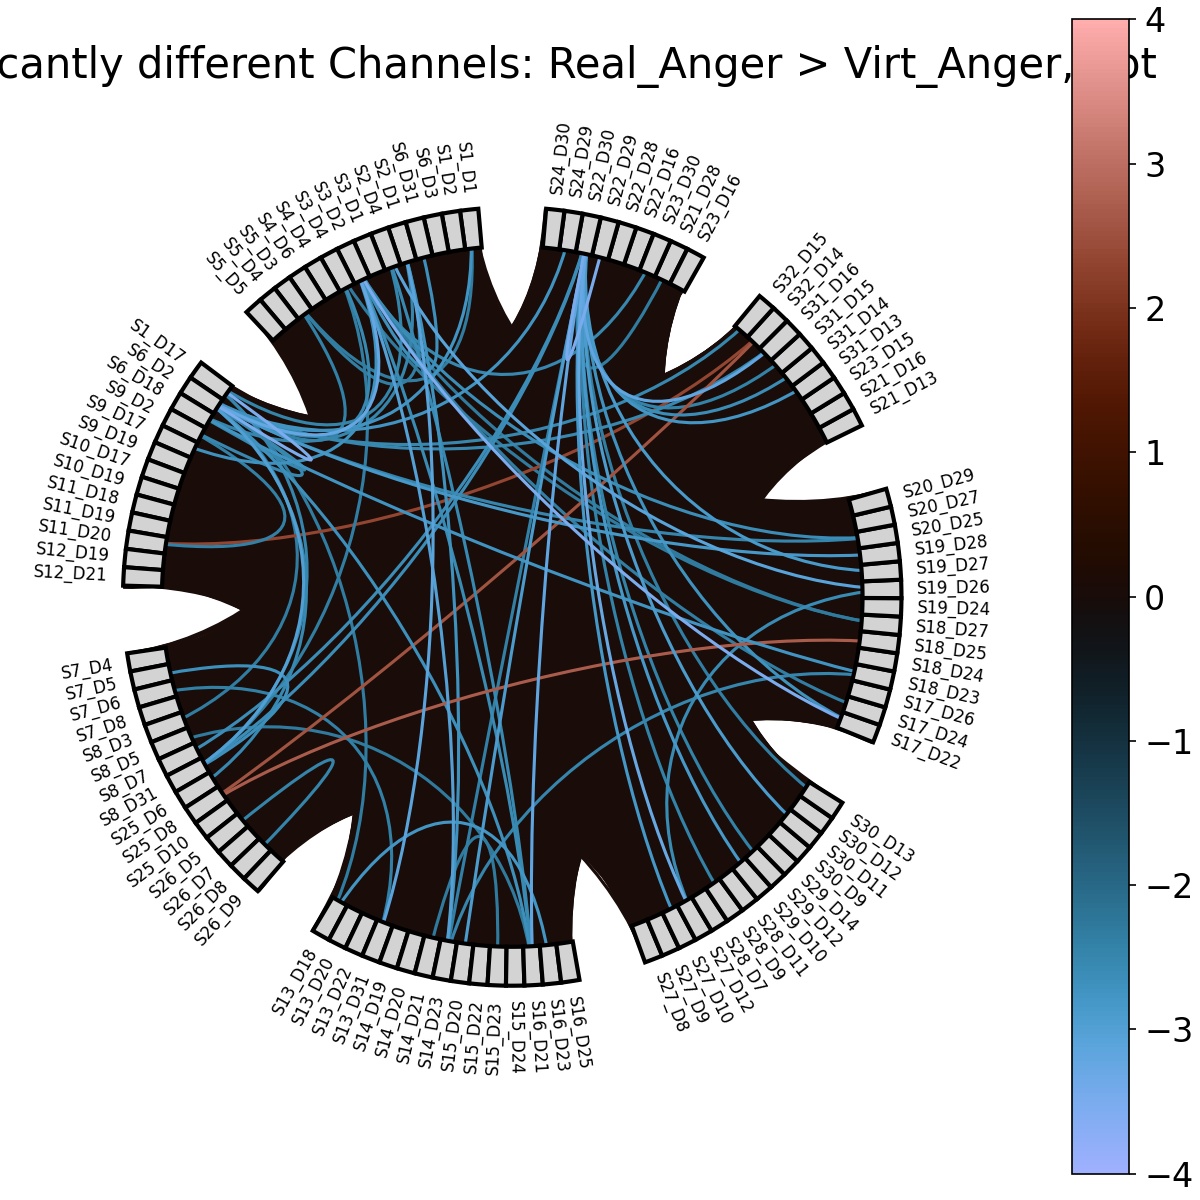
\includegraphics[width=0.3\textwidth]{C:/Users/super/OneDrive - Ontario Tech University/fNIRS_Emotions/plots/spectral_connectivity_time/chord_plots/group_level_t_tests_roi/face_type_emotion_Real_Anger_Virt_Anger.png}
  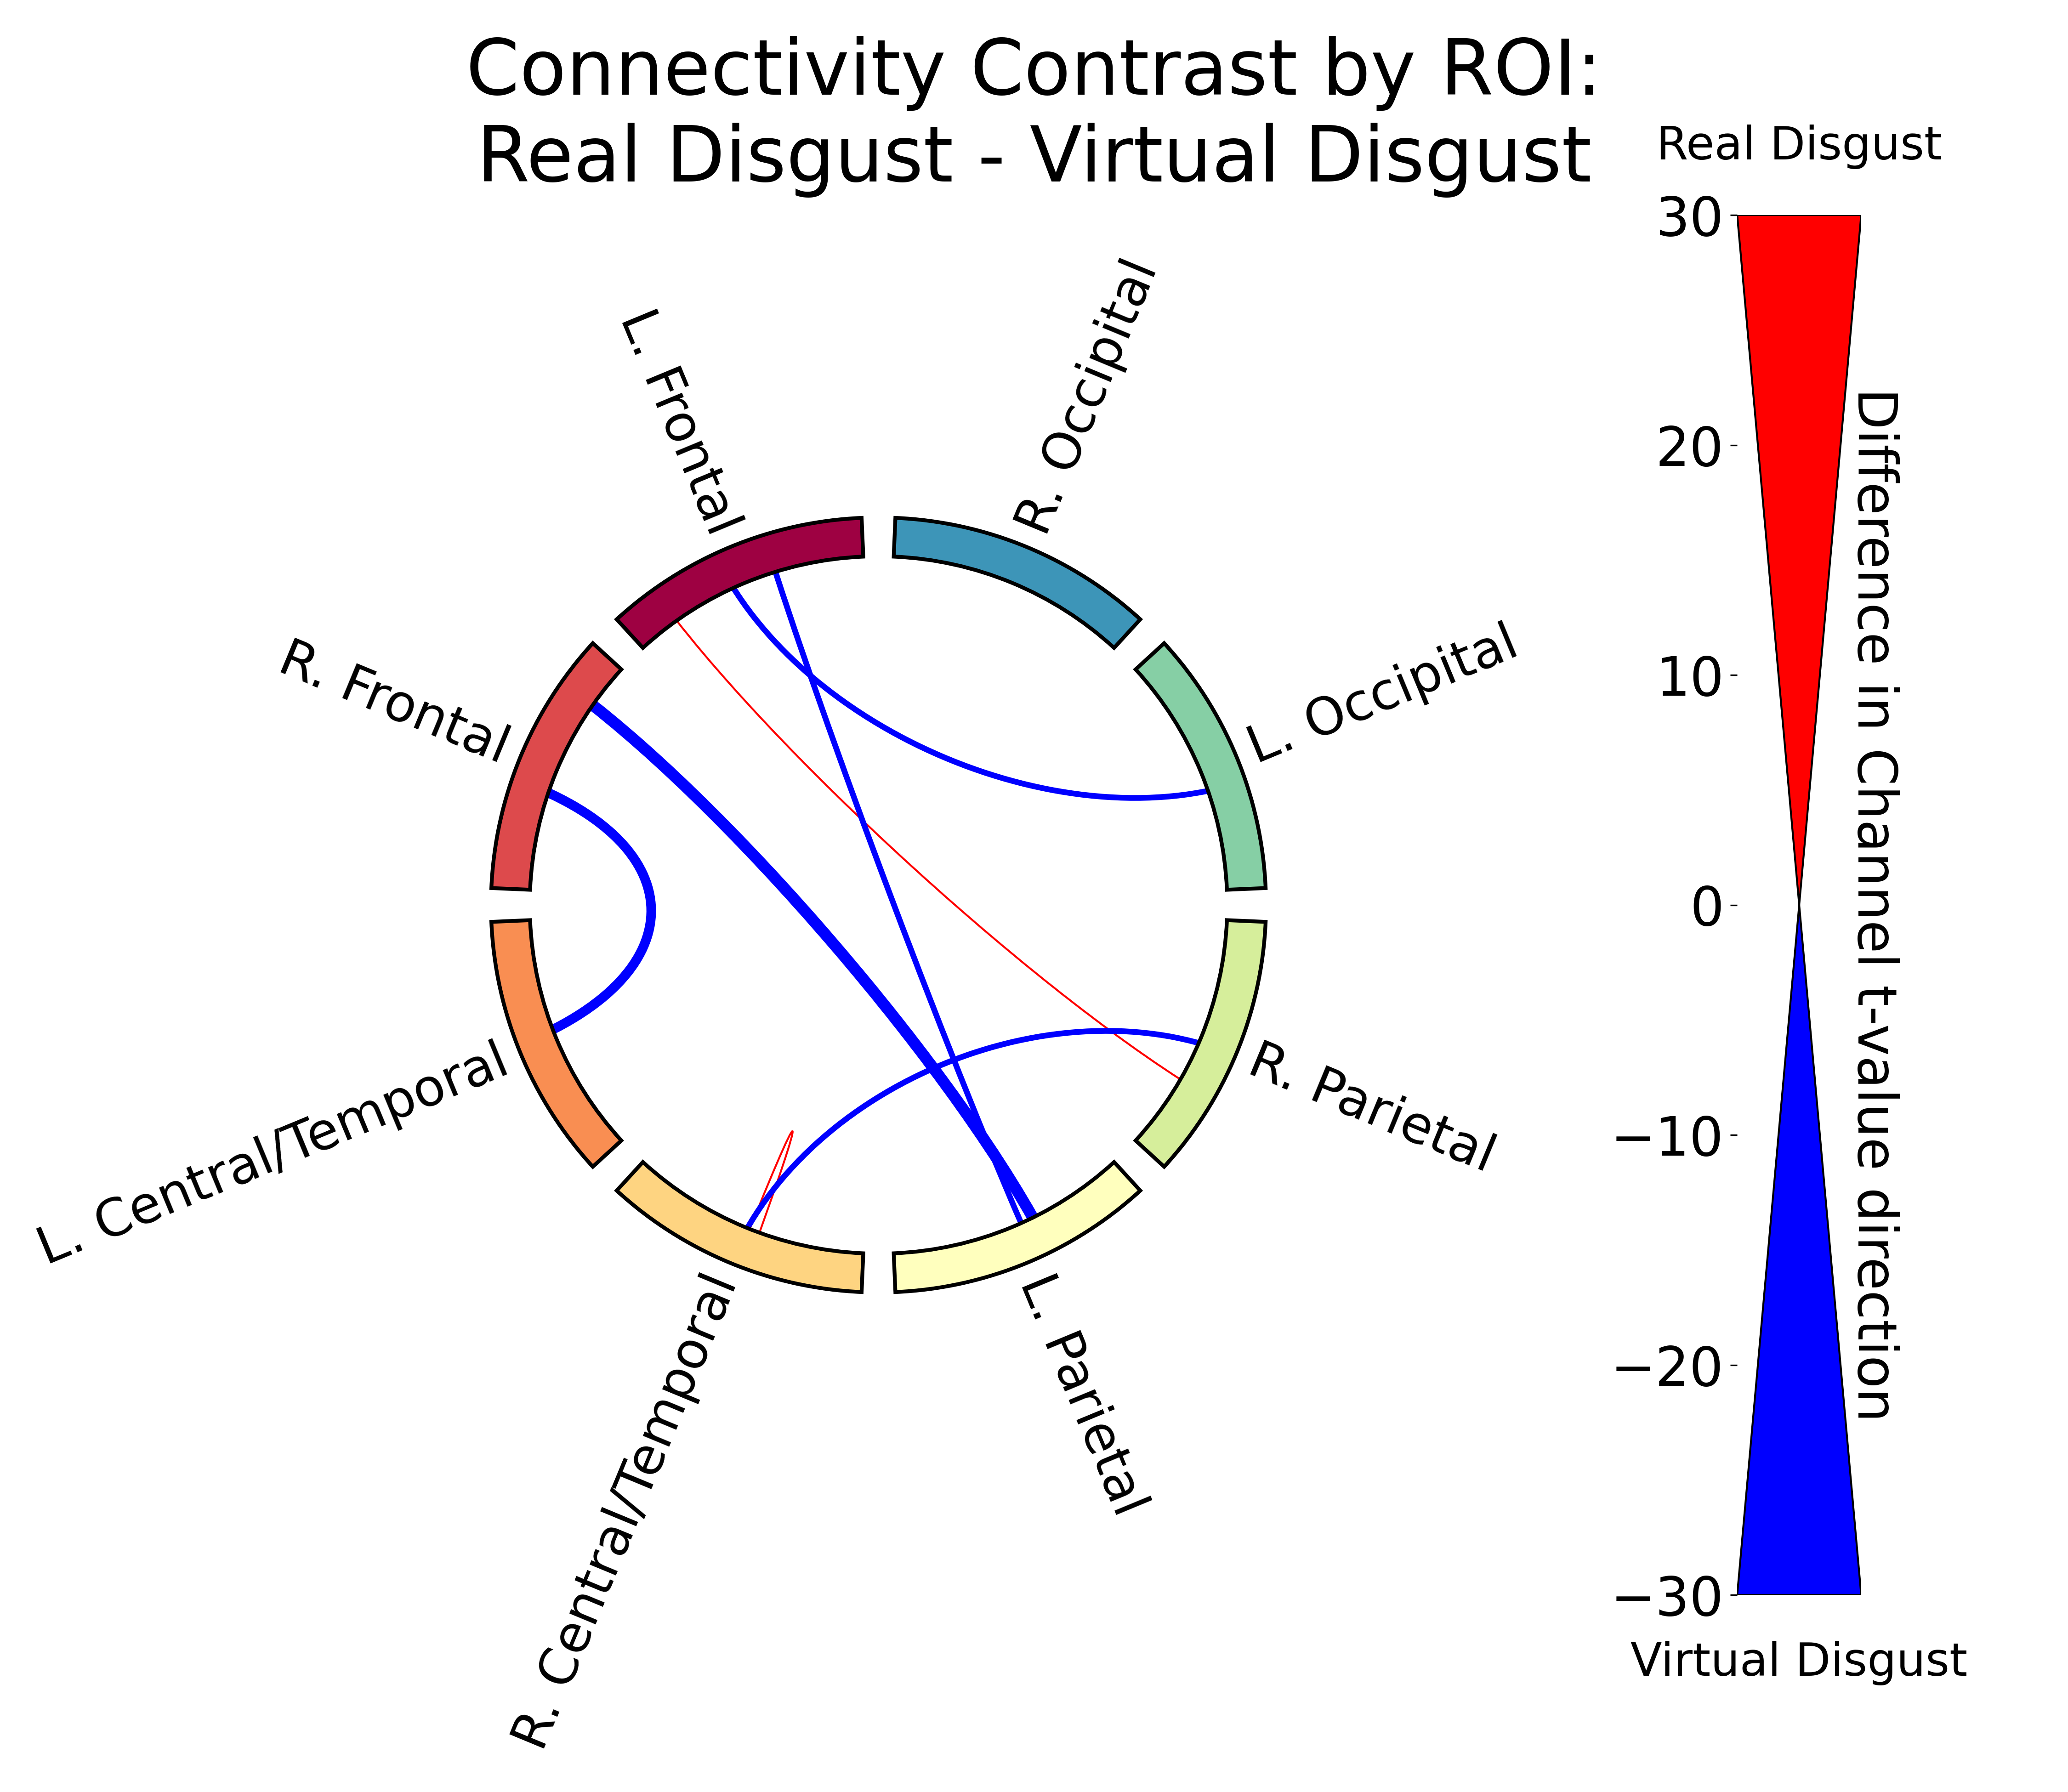
\includegraphics[width=0.3\textwidth]{C:/Users/super/OneDrive - Ontario Tech University/fNIRS_Emotions/plots/spectral_connectivity_time/chord_plots/group_level_t_tests_roi/face_type_emotion_Real_Disgust_Virt_Disgust.png}
  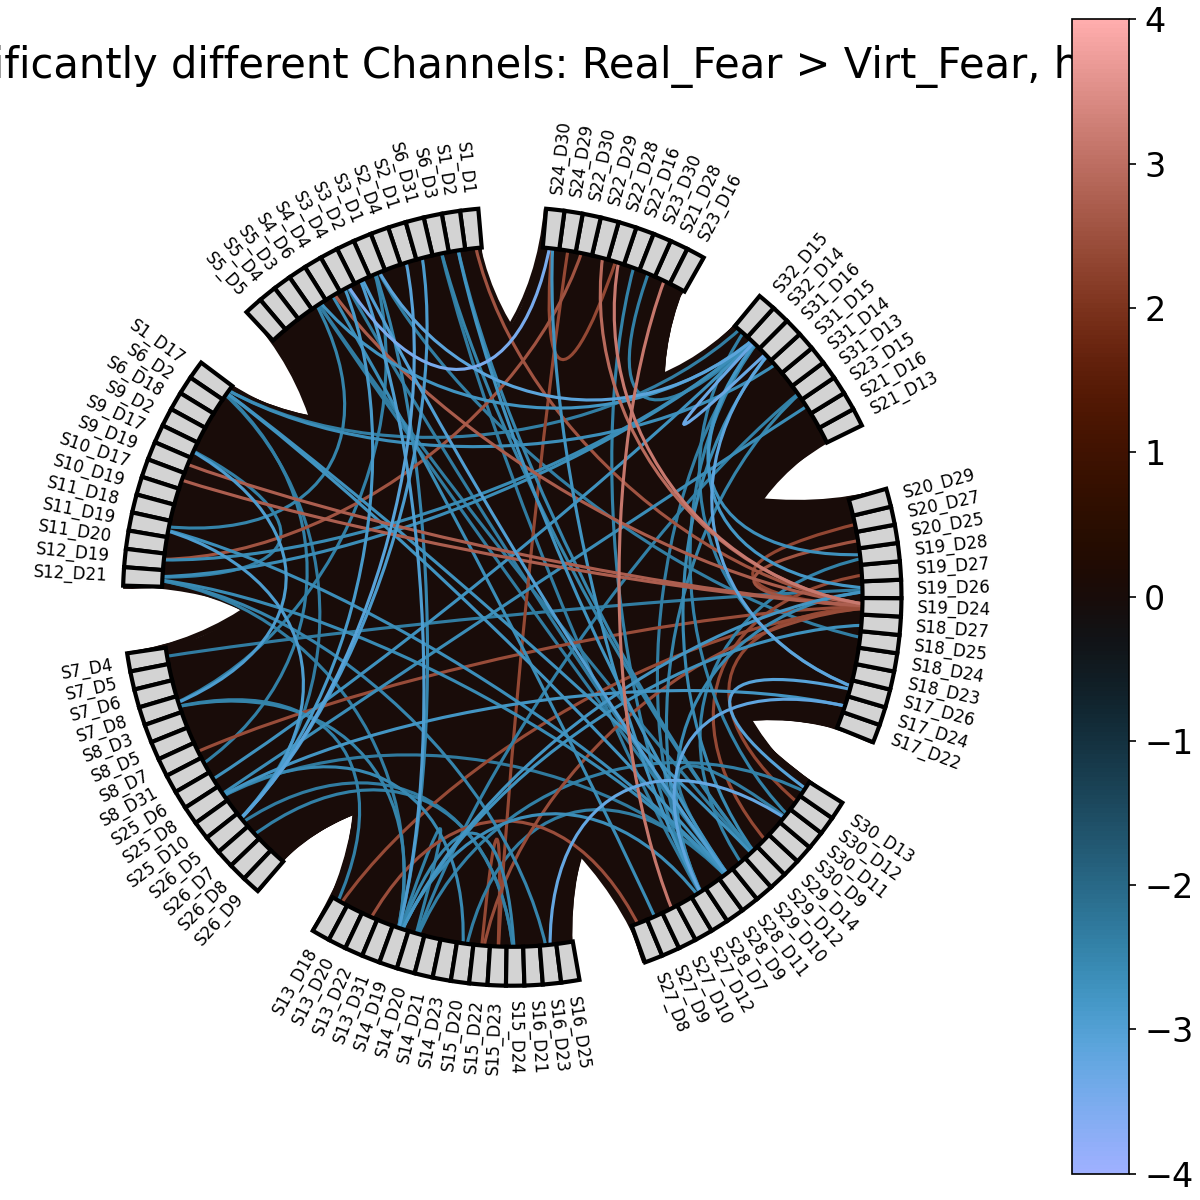
\includegraphics[width=0.3\textwidth]{C:/Users/super/OneDrive - Ontario Tech University/fNIRS_Emotions/plots/spectral_connectivity_time/chord_plots/group_level_t_tests_roi/face_type_emotion_Real_Fear_Virt_Fear.png}
  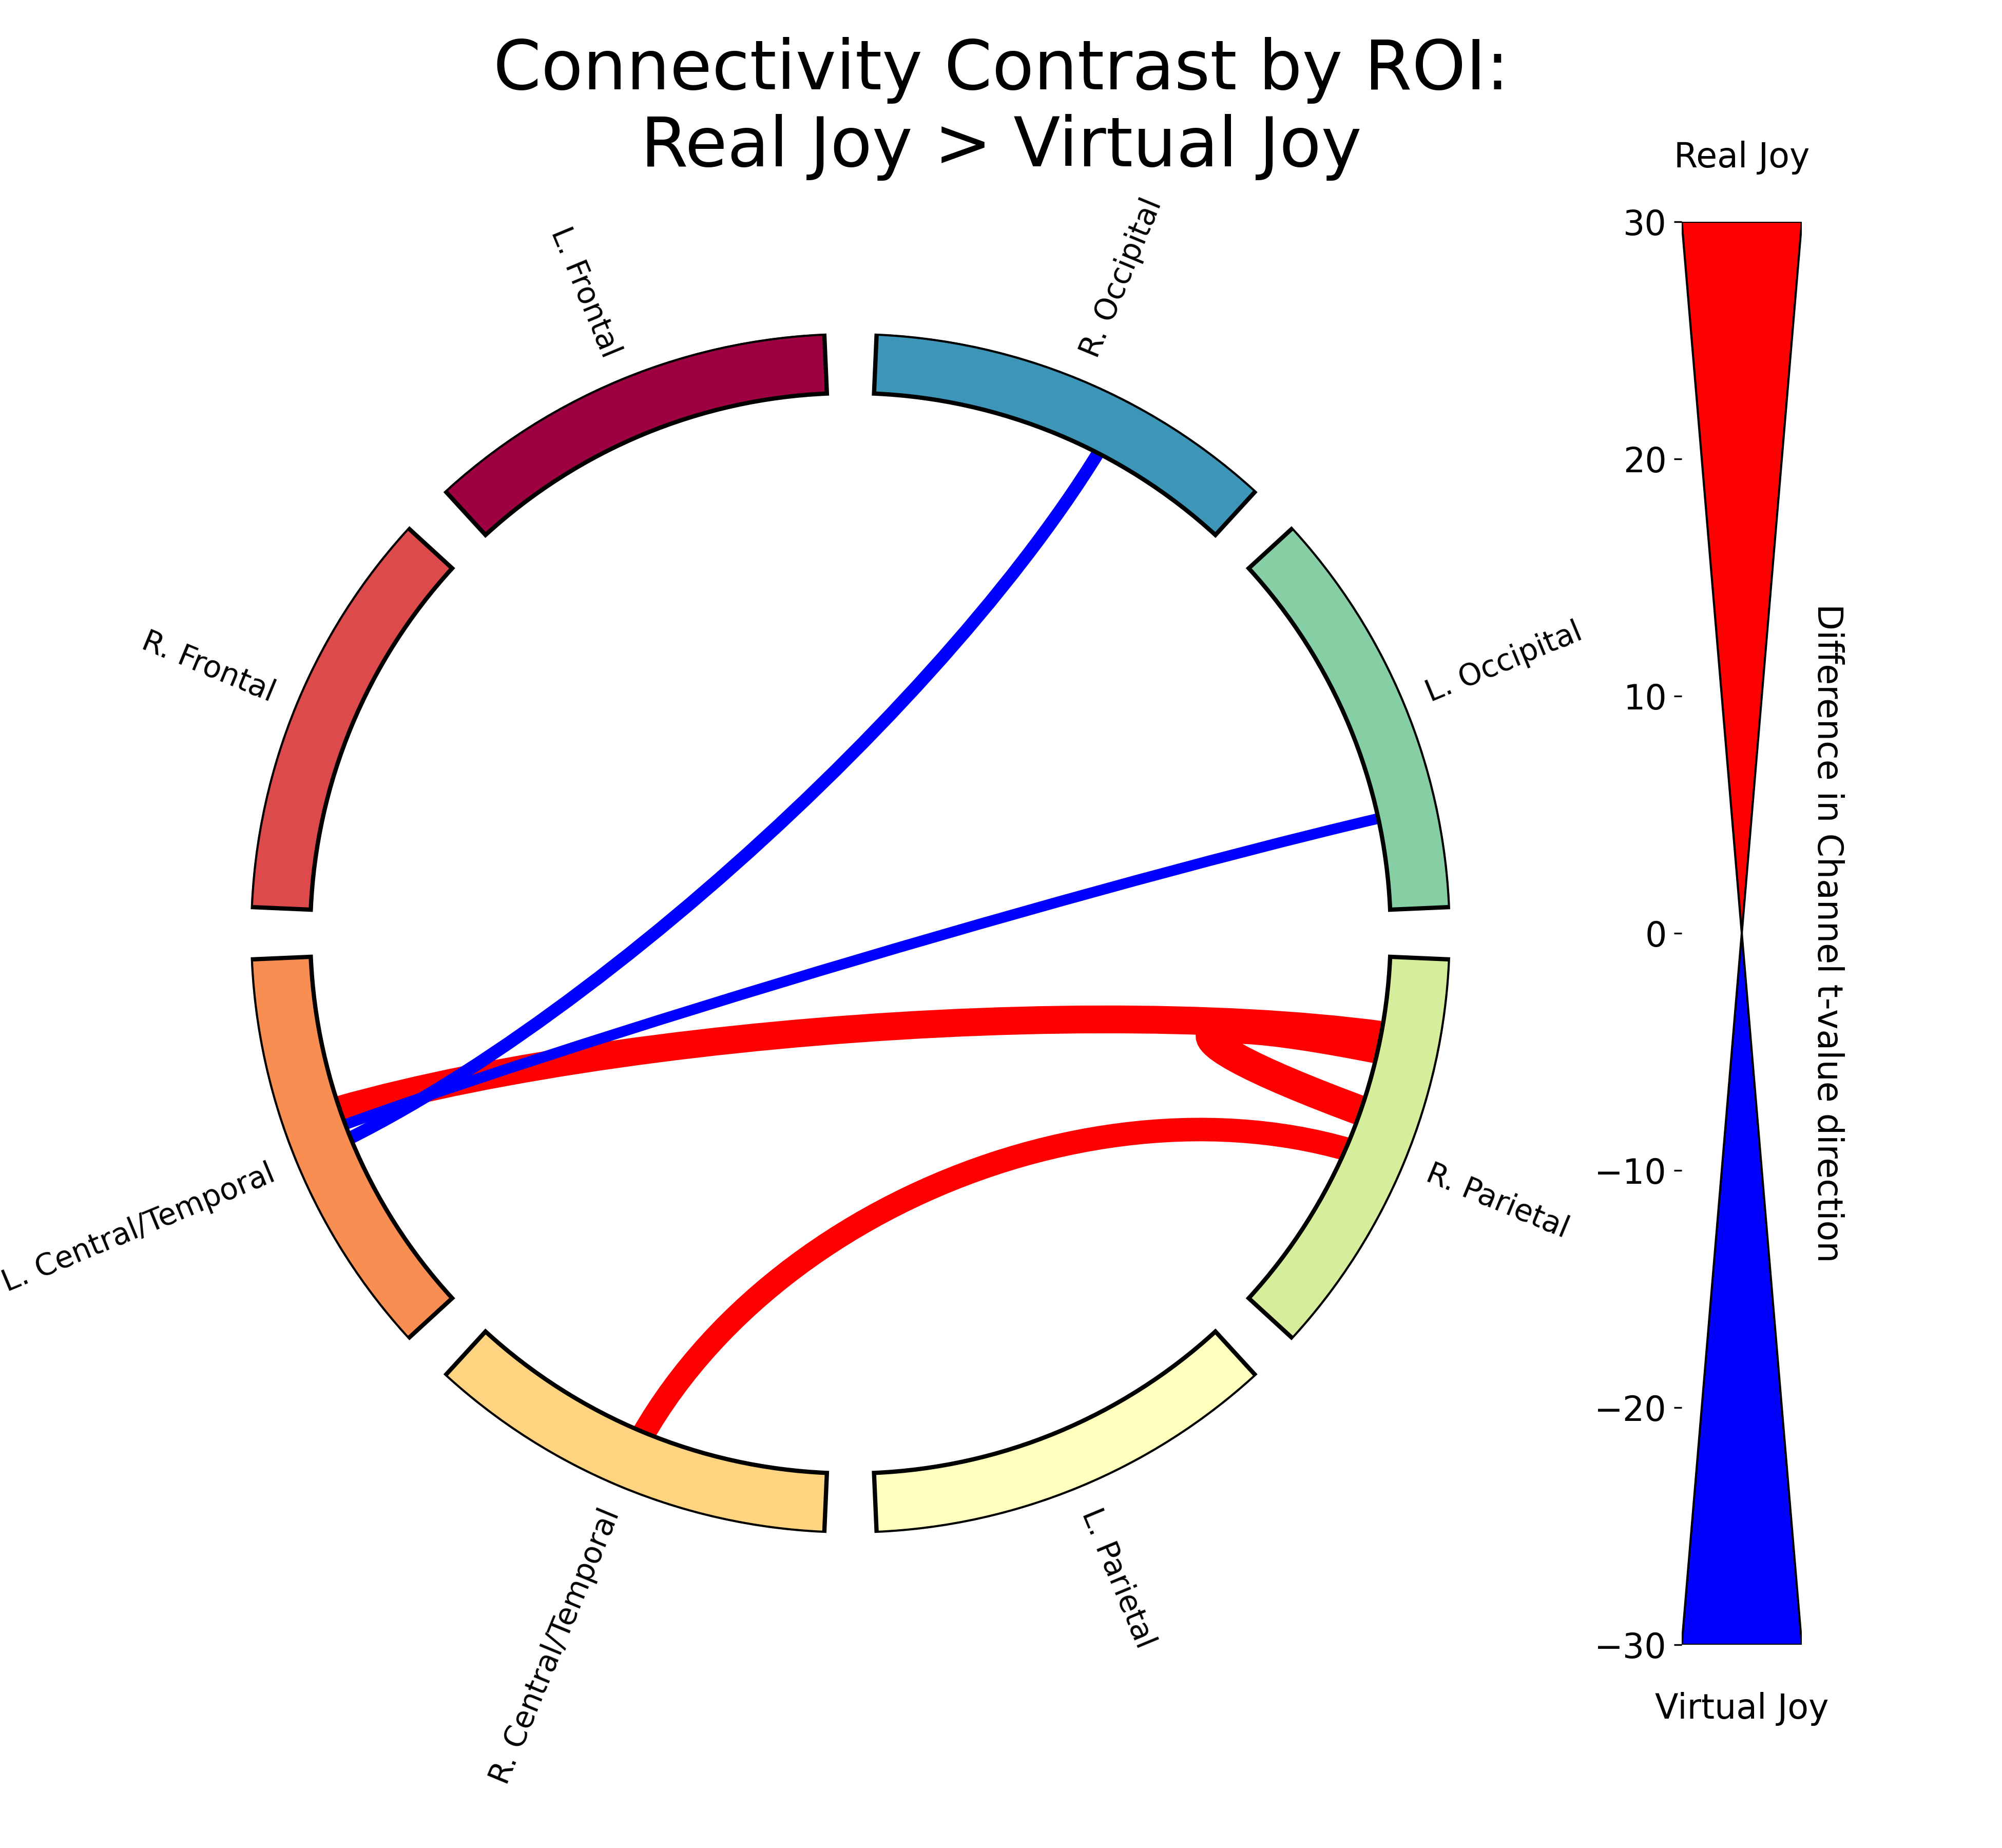
\includegraphics[width=0.3\textwidth]{C:/Users/super/OneDrive - Ontario Tech University/fNIRS_Emotions/plots/spectral_connectivity_time/chord_plots/group_level_t_tests_roi/face_type_emotion_Real_Joy_Virt_Joy.png}
  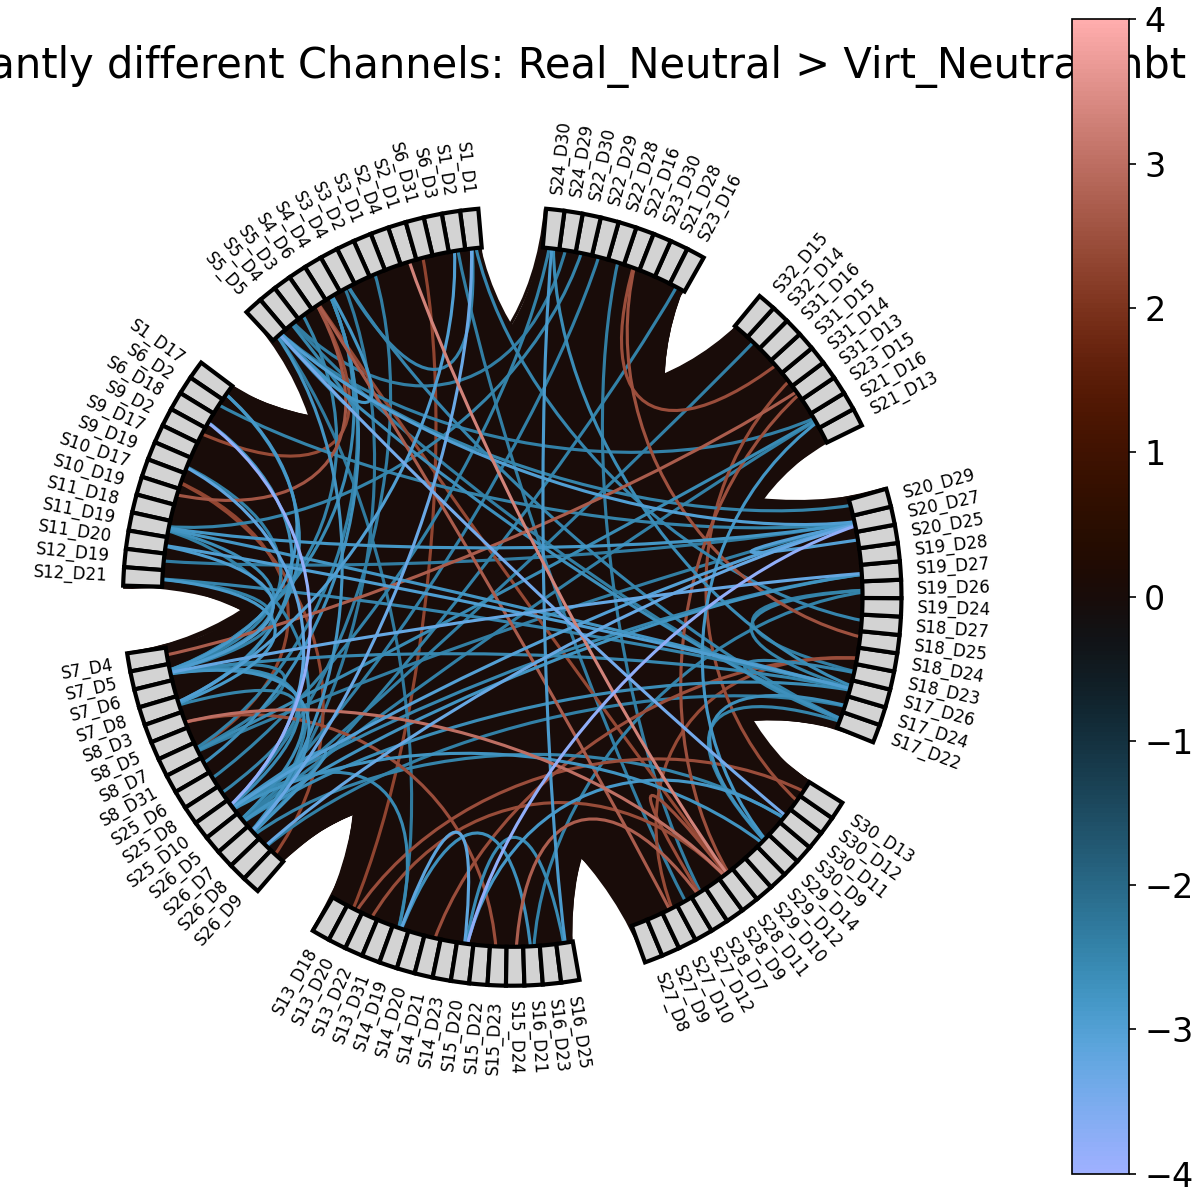
\includegraphics[width=0.3\textwidth]{C:/Users/super/OneDrive - Ontario Tech University/fNIRS_Emotions/plots/spectral_connectivity_time/chord_plots/group_level_t_tests_roi/face_type_emotion_Real_Neutral_Virt_Neutral.png}
  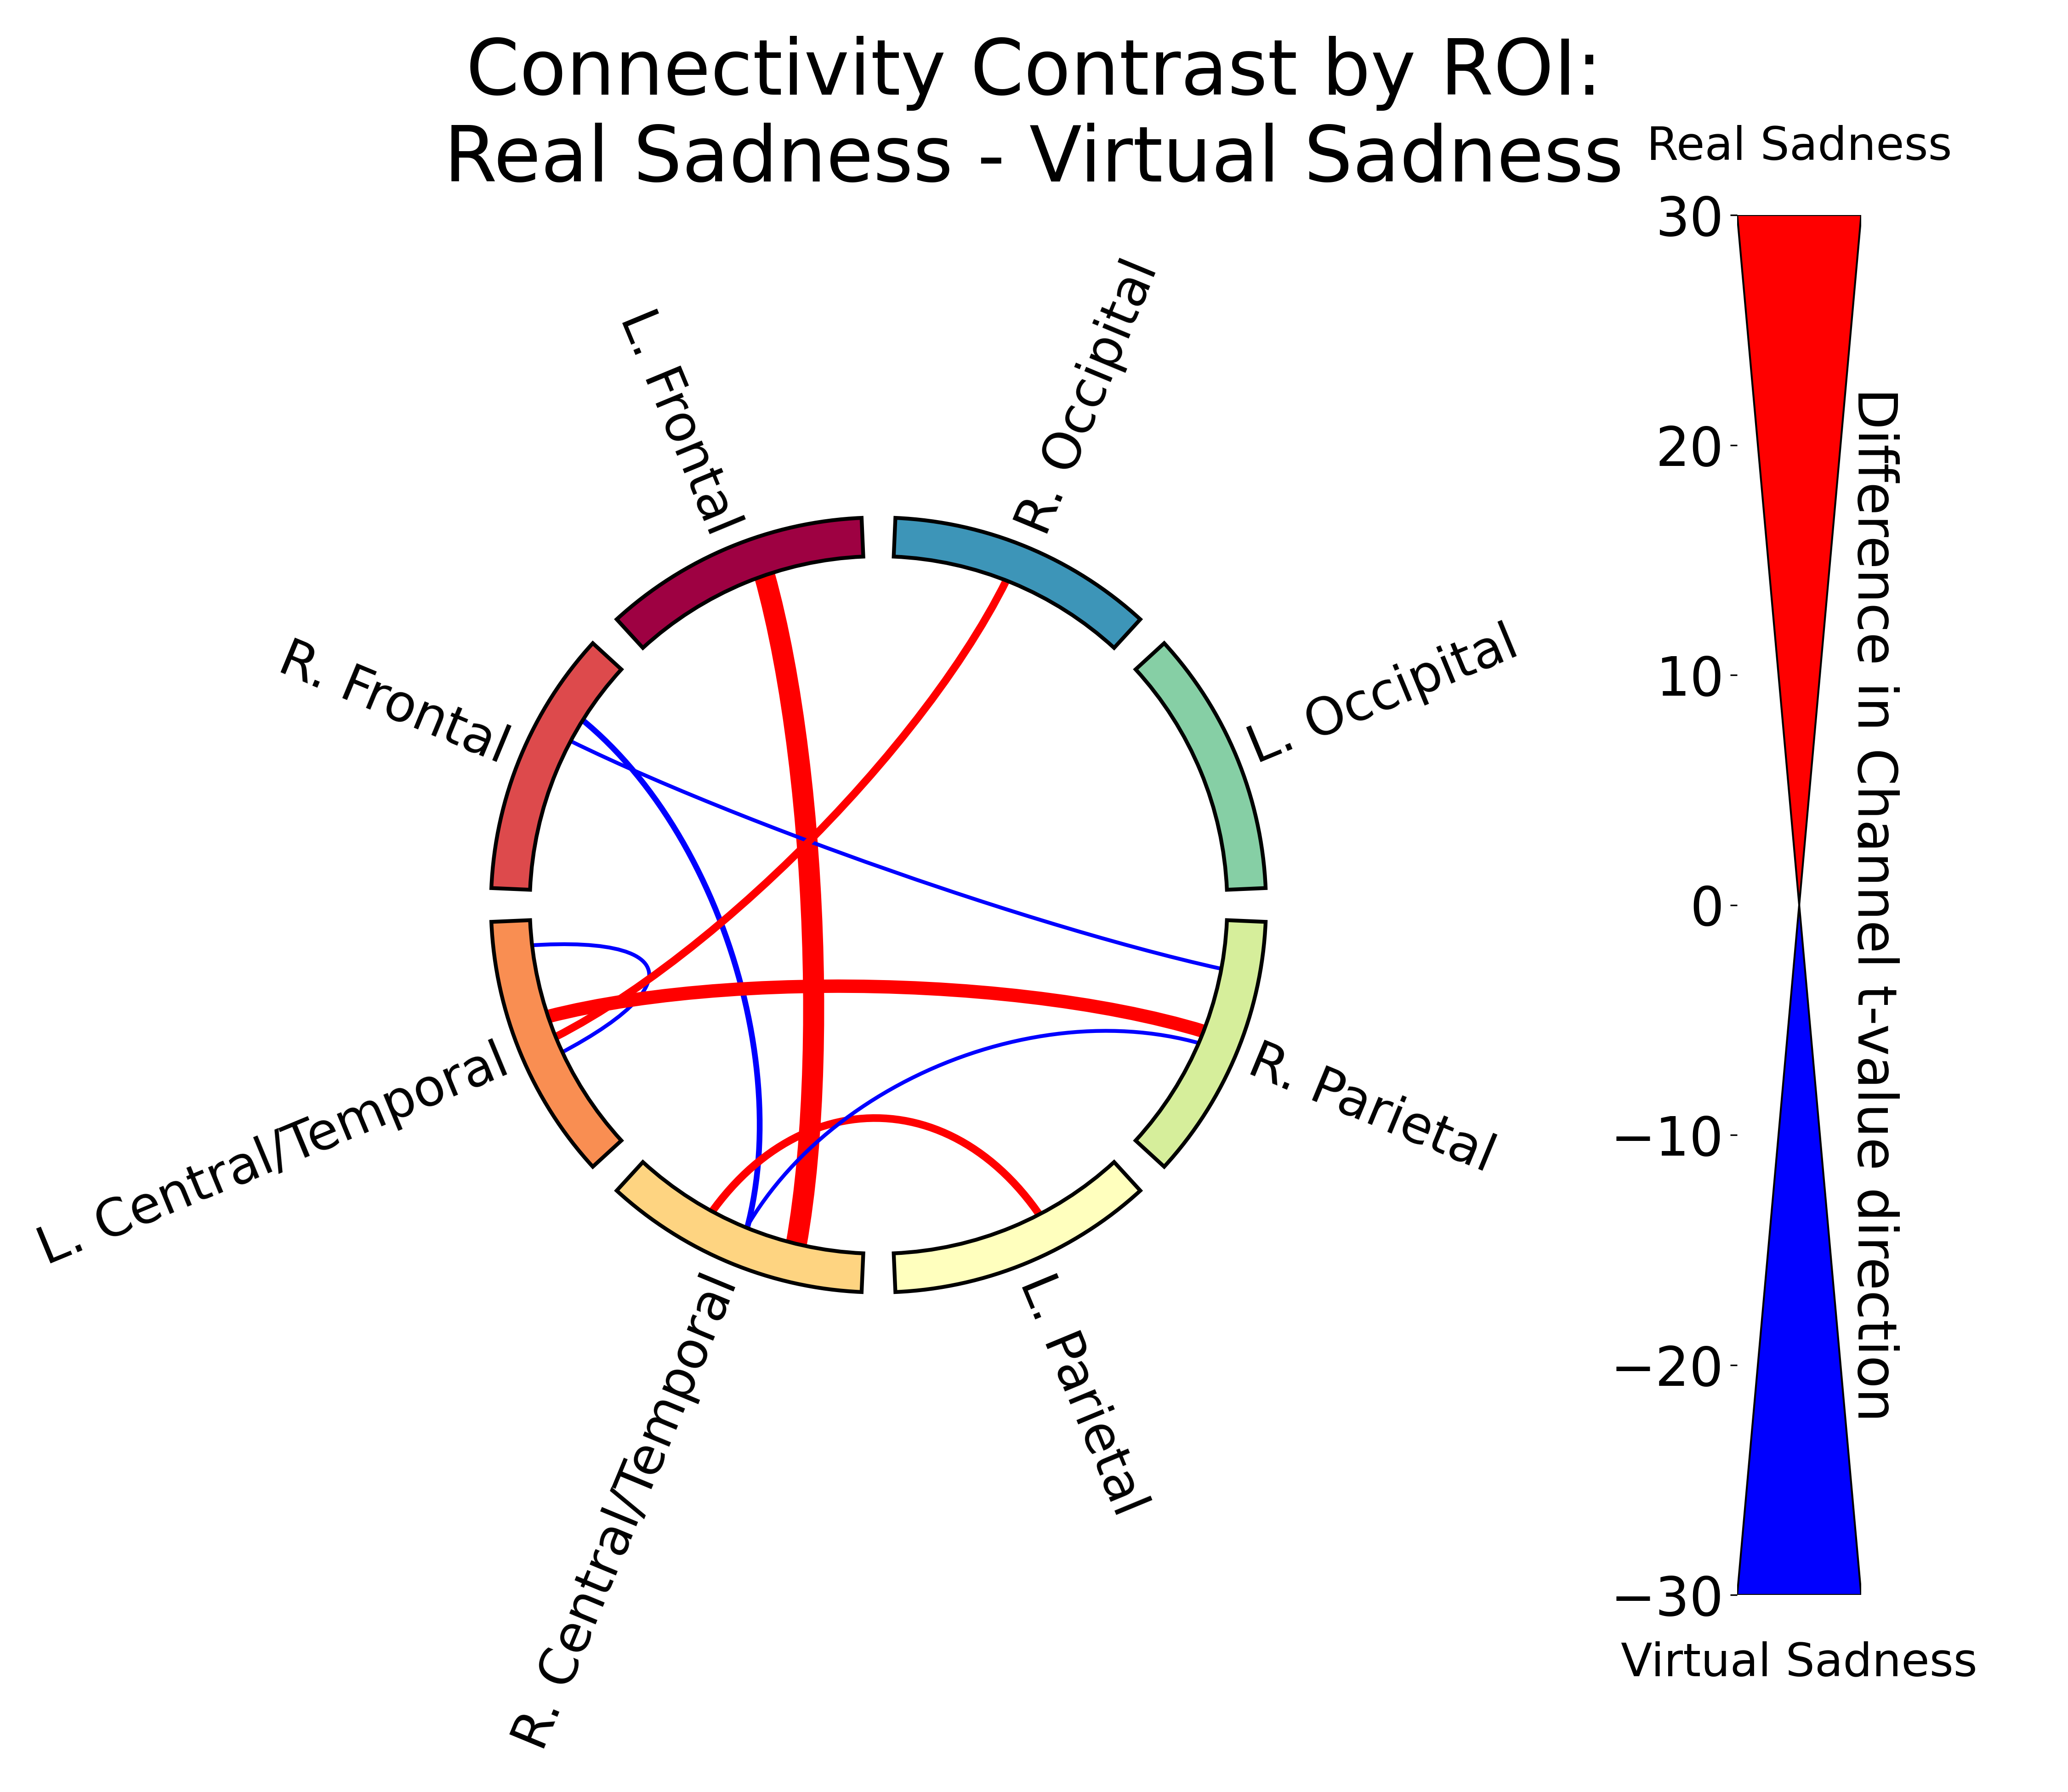
\includegraphics[width=0.3\textwidth]{C:/Users/super/OneDrive - Ontario Tech University/fNIRS_Emotions/plots/spectral_connectivity_time/chord_plots/group_level_t_tests_roi/face_type_emotion_Real_Sadness_Virt_Sadness.png}
  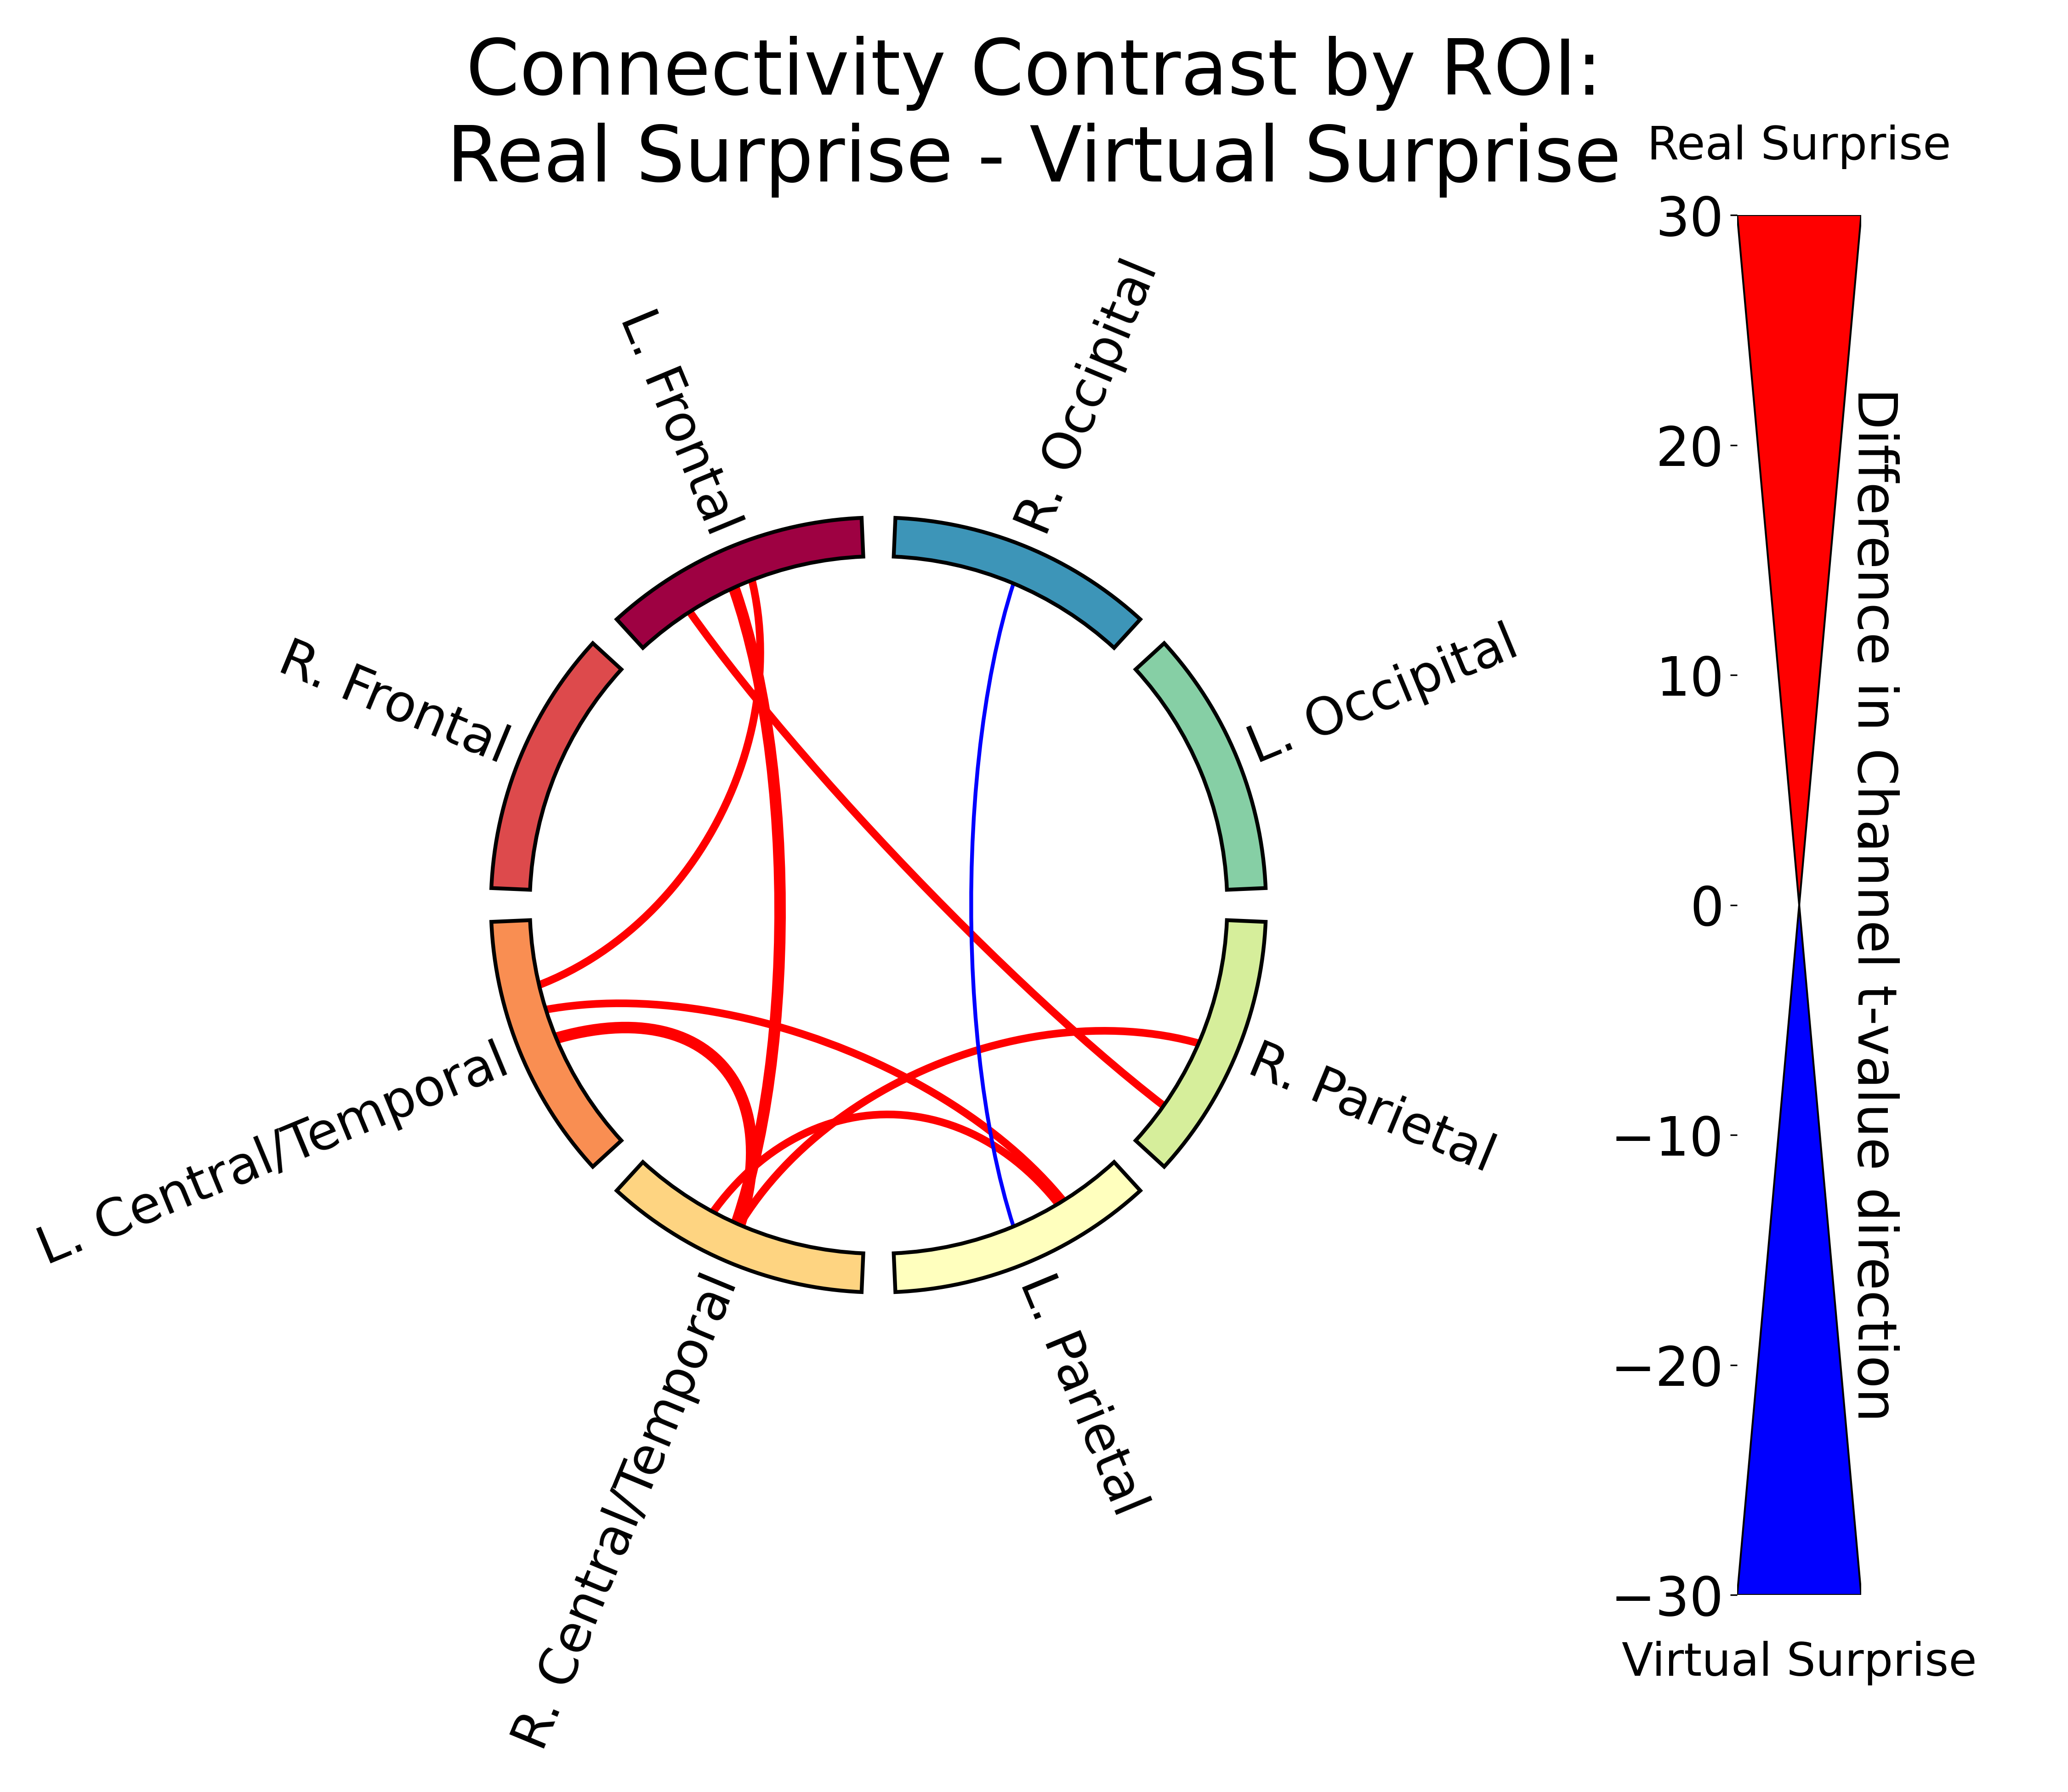
\includegraphics[width=0.3\textwidth]{C:/Users/super/OneDrive - Ontario Tech University/fNIRS_Emotions/plots/spectral_connectivity_time/chord_plots/group_level_t_tests_roi/face_type_emotion_Real_Surprise_Virt_Surprise.png}
  \caption[FC: Face Type \texorpdfstring{$\times$}{x} Emotion Contrasts]{Functional connectivity results for the contrast between real and virtual conditions within each emotion.
  Same concept as explained in figure \ref{fig:fc_real_vs_virtual}. }
  \label{fig:fc_real_vs_virtual_emotion_analysis}
\end{figure}

The interaction of face type with emotion (Real $>$ Virt within each emotion as shown in \ref{fig:fc_real_vs_virtual_emotion_analysis}) revealed significant differences in functional connectivity across both face types within each emotion.
For Anger, Disgust, Fear, and Neutral, virtual faces showed higher connectivity across most ROI's compared to real faces, whereas for Joy, Sadness, and Surprise, real faces showed higher connectivity across most ROI's compared to virtual faces.
Like the GLM results, this indicates that the neural response to emotional expressions is modulated by the realism of the face stimuli, with different patterns of connectivity observed for each face type \texorpdfstring{$\times$}{x} emotion interaction.

The full table of the functional connectivity contrasts for all main effects and interactions can be found in Appendix \ref{tab:appendix_fc_emotion_analysis}.

\section{Memory Task Results}
\begin{figure}[H]
  \centering
  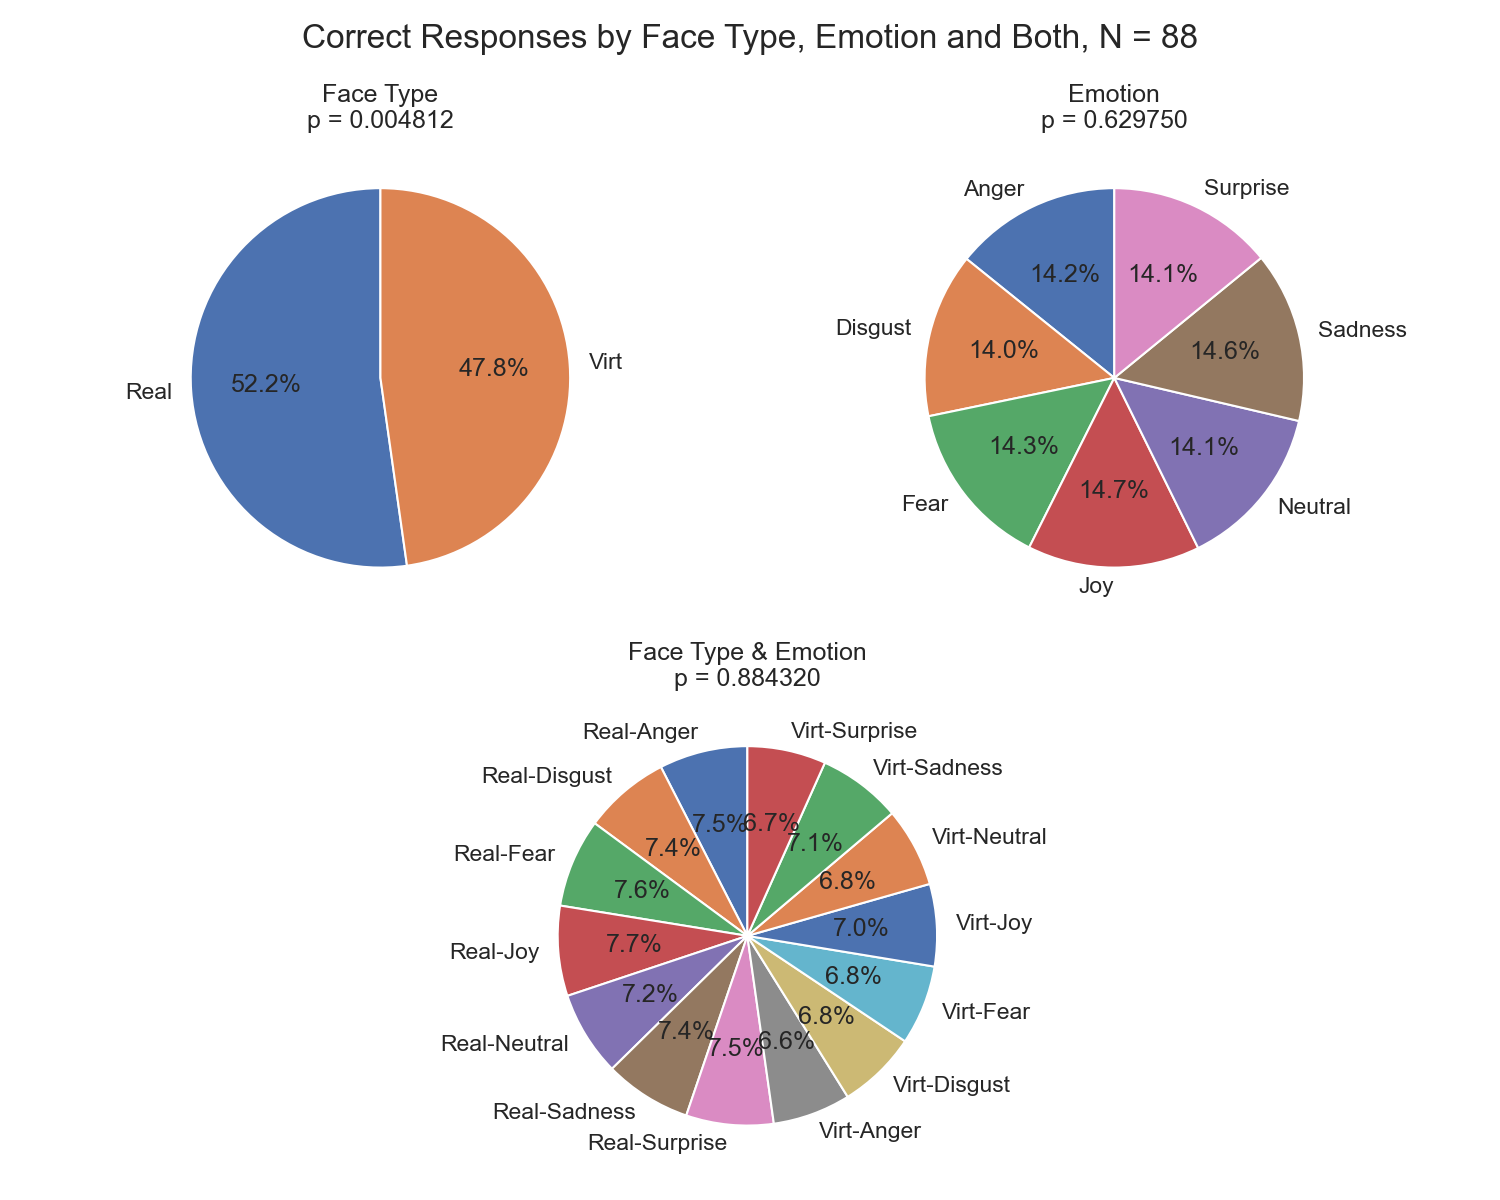
\includegraphics[width=0.9\textwidth]{C:/Users/super/OneDrive - Ontario Tech University/fNIRS_Emotions/plots/behavioural_responses/correct_responses_by_face_type_emotion.png}
  \caption[Correct Memory Task Responses by Face Type and Emotion]{Proportion correct by condition in the memory task, plotted separately for real and virtual faces, for each emotion, and the interaction between face type and emotion. 
  The $p$-values indicate the significance of the main effects and interaction. }
  \label{fig:memory_task_results}
\end{figure}

A two-way Type III ANOVA (as described in \ref{sec:memory_task_analysis}) was conducted to examine the main effects and interaction on memory performance (proportion correct). 
Figure \ref{fig:memory_task_results} shows accuracy by face type/emotion and their interaction.
The analysis revealed a significant main effect of face type, $F(1,4802)=7.96$, $p=0.0048$, indicating that memory performance was higher for real faces compared to virtual faces. 
There was no significant main effect of emotion, $F(6,4802)=0.83$, $p=0.55$, nor a significant interaction between face type and emotion, $F(6,4802)=0.46$, $p=0.84$. 
These findings suggest that while the realism of the face influences memory performance, the specific emotional expression does not have a significant impact on memory accuracy.
The full ANOVA table is shown in Appendix \ref{tab:appendix_memory_task_anova}.

\chapter{Discussion}
The present study aimed to characterize how the human brain processes emotional expressions displayed by real versus virtual faces, using fNIRS to measure both activation and functional connectivity. 
We sought to determine whether face realism modulates neural responses to different emotions, and whether these effects extend beyond local activation to distributed network interactions. 
By directly comparing hemodynamic responses to real and virtual faces across a range of basic emotions, our goal was to provide novel insights into the neural mechanisms underlying emotional face perception in the context of increasing virtual social interactions.

\section{Left occipital activation for virtual faces}
Our finding that virtual faces elicit greater left occipital activation compared to real faces aligns with evidence that face realism modulates visual processing in a complex manner. 
\cite{schindler_differential_2017} showed that the N170 EEG component, reflecting early face perception, is influenced by perceived realism in a u-shaped fashion, while the later Late Positive Potential (LPP) increases continuously with face realism. 
Notably, the N170 generators differ between highly stylized and very realistic faces, suggesting distinct neural processes are engaged depending on realism. 
The LPP enhancement with increasing realism is associated with broader occipito-parietal activity, converging with our fNIRS results that show stronger left occipital activation for virtual faces.
This indicates that the neural response to virtual faces reflects the perceptual demands of artificial stimuli in the occipital area. 
Face perception reliably activates the lateral fusiform gyrus, typically bilaterally but most robustly on the right hemisphere \cite{haxby_distributed_2000}. 
This region shows greater responses to faces than to non-face objects. 
Although fNIRS cannot directly measure deep structures like the fusiform gyrus, it is close enough to detect activity in adjacent occipital regions that are functionally connected to the fusiform and contribute to early stages of face processing.
Our observed higher left occipital activation for virtual faces compared to real faces may then reflect increased perceptual demands in upstream visual areas when viewing virtual faces.

\section{Higher Activation for Neutral and Surprise}
Our results showed that neutral and surprise facial expressions elicited stronger activation than other emotions, particularly in the occipital, right parietal, and left central/temporal regions.
There is consistent evidence of increased brain activation in response to neutral and surprise facial expressions, sometimes even exceeding responses to more overt emotional expressions.
\cite{moser_amygdala_2007} found both avatar and human emotional faces activated regions typically involved in emotion processing, such as the bilateral amygdala, fusiform gyri, cerebellum, and superior temporal gyrus. 
Notably, neutral face conditions also produced strong amygdala activation. 
This suggests that the amygdala may not only respond to emotional intensity, but also to the social relevance of faces in general. 
This aligns with previous findings showing that some neurons in the temporal lobe and amygdala are tuned to detect faces rather than specific emotions.
\cite{keslerwest_neural_2001} used fMRI to compare responses to neutral and scrambled faces. 
It revealed robust activation in regions like the fusiform gyri, amygdalae, entorhinal cortices, and superior temporal sulcus during neutral face viewing. 
These findings confirm that emotionally neutral faces still engage core regions involved in face perception and social processing, likely due to their ambiguous or uncertain emotional content.
\cite{westgarth_systematic_2021} reviewed prior fNIRS and fMRI literature and found inconsistent results for emotional face processing in the PFC. 
While some studies reported increases in oxygenated hemoglobin in regions like the medial and ventral PFC, others showed decreases or no change, depending on the emotion or brain region. 
Our own fNIRS findings showed that both neutral and surprise expressions evoked stronger responses than other emotions, possibly because neutral and surprise faces are more ambiguous and require more cognitive effort to interpret, especially in social contexts.
These findings and our own challenge the assumption that strongly emotional faces always produce the strongest brain responses. 

\section{Stronger connectivity for real faces}
Our functional connectivity analysis revealed distinct neural connectivity patterns associated with processing both real and virtual faces, suggesting that the realism of facial stimuli modulates the underlying brain network dynamics during face processing.
We observed stronger connectivity when processing real faces across parietal, frontal, and central/temporal regions. 
\cite{hirsch_frontal_2017} conducted a two-person fNIRS hyperscanning study finding cross-brain coherence in left frontal, temporal, and parietal regions during social interaction/live eye-to-eye contact. 
A notable limitation of their study was that there was no occipital coverage, but given that our findings found no significant connectivity differences in the left or right occipital region, this suggests that the occipital region may not be as involved in these processes.
These findings further support the notion that real face recognition engages a broader and more coherent neural network. 
\cite{tarchi_electroencephalographic_2023} further supports our observation of stronger neural connectivity for real faces, as EEG data revealed statistically significant differences in brain activation between real and synthetic stimuli. 
The observed discrimination ability, where participants correctly identified real versus synthetic faces with 77\% accuracy, suggested a greater sensitivity to facial authenticity. 
Together, these results align with our connectivity analysis, reinforcing the notion that real faces engage brain networks, particularly in emotional and cognitive processing regions, more robustly than synthetic counterparts.

\section{Stronger connectivity for Fear}
Among emotions, Fear (followed closely by Anger) elicited the strongest connectivity compared to the other emotions, especially for connections involving the left central/temporal cortex across frontal and parietal regions. 
Fearful faces signal potential threat, and the interpretation of these cues depends on contextual factors, whereas Anger signals the source of threat. 
\cite{cushing_neurodynamics_2018} found that fear processing is engages the amygdala, particularly when eye gaze is not directed at the viewer compared to when it is.
\cite{jamieson_differential_2021} found that the connectivity from the amygdala to the dorsolateral prefrontal cortex (dlPFC) differs when processing fearful versus sad facial expressions. 
They reported increased connectivity when processing fearful faces compared to sad faces, attributing this to the higher salience and arousal associated with fear \citep{adolphs_biology_2013}.
This pattern resonates with our emotion connectivity summary heatmap (Figure \ref{fig:fc_emotion_summary_analysis}), where fearful faces show robust network engagement relative to others. 
Additionally, \cite{liang_multivariate_2018} found that facial emotion expressions can be successfully decoded from functional connectivity patterns, and the networks identified include brain regions beyond the conventional face-selective areas. 
This finding supports the notion that emotional face processing involves distributed networks rather than isolated regions, aligning with our connectivity results.
Anger and Joy also produced notably strong connectivity, clustering with Fear in our summary heatmap. 
Lower connectivity for Disgust, Sadness, Surprise, and Neutral faces supports the idea that these emotions have lower arousal or social salience compared to Fear, Anger, and Joy.

Our regional analysis found minimal connectivity differences among left and right occipital ROI across emotions, while central/temporal and parietal regions varied strongly (Figure \ref{fig:fc_region_summary_analysis}).
This fits with models of face perception, where early visual areas (e.g., occipital face area) feed into higher-level hubs like the fusiform face area. 
\cite{underwood_networks_2021} that effective connectivity analyses reveal dynamic modulation between occipital, frontal, and subcortical regions, but that early visual areas remain relatively stable across emotion conditions, with emotional discrimination only arising in higher circuits. 
This suggests that while occipital areas are crucial for initial face processing, the emotional nuances of faces are primarily encoded in more distributed networks involving parietal and central/temporal regions.

\section{Superior memory for real faces}
Our findings align with a growing consensus: real faces are remembered more accurately than artificial ones, even though both are processed as faces. 
\cite{balas_artificial_2015} found that artificial faces are remembered less efficiently and discriminated slightly worse than real faces, supporting the hypothesis that "out-group" faces, those that are less familiar or realistic, are processed differently.
Complementing this, \cite{katsyri_those_2018} showed that virtual faces trigger higher false alarm rates, a sign of reduced memory specificity, despite matched visual features and equivalent overall recognition sensitivity. 
Participants also rated these faces as eerier, highlighting a connection between reduced perceptual expertise and the uncanny valley experience. 
This suggests that artificial faces engage face-specific processing yet are represented more weakly in memory. 
\cite{katsyri_amygdala_2020} found that real faces, compared to computer-generated (CG) faces, were associated with poorer performance in an implicit catch trial task. 
The effect was interpreted as reflecting an involuntary attentional response toward human faces, which are highly familiar and socially salient visual stimuli. 
The automatic allocation of attention to real faces may have interfered with participants' ability to withhold a motor response until the catch stimulus appeared, as required by the task. 
This is consistent with our finding that participants performed better on our memory task for real faces than virtual ones.
Enhancing familiarity through exposure \citep{park_individuals_2021} or increasing realism could help bridge this memory gap. 
Neuroscientific and evolutionary theories also propose that the human brain includes specialized modules (e.g., the fusiform face area), are highly attuned to natural facial features \citep{burke_evolution_2013}. 
These modules are refined by experience and optimized for identity recognition, which may not be fully triggered by virtual faces, due to limited exposure or differences in visual features.
This may signal evolutionary utility in processing real, familiar faces, and why virtual faces, even when perceived as faces, do not engage the same neural mechanisms as real faces.

\section{Limitations and Future Directions}
This study was the first to use fNIRS to examine neural responses to real versus virtual emotional faces, providing novel insights into how face realism and emotion interact in the brain.
However, several limitations should be acknowledged.
First, since we recruited only from Ontario Tech University's undergraduate student body, our sample of students were limited to that relatively young age range and community, and likely are more educated and technologically savvy than the general population.
This may limit the generalizability of our findings to broader populations, particularly older adults or those with less exposure to virtual characters/avatars.
As well, many participants did not pass our signal quality checks, due to reasons discussed in \cite{holmes_opening_2024}, such as hair color/texture affecting the signal quality. 
Additionally, our sample was predominantly female, which may have influenced our results as \cite{weisenbach_reduced_2014} found that females and males may differ in their accuracy and sensitivity when categorizing facial emotions; for example, females have been shown to outperform males in identifying fearful faces.
\cite{keslerwest_neural_2001} also found men have a differential neural response depending upon the emotion presented. 
Future studies should include a wider range of participants, ideally representing the general population. 

Second, since the virtual faces used in this study were all from one dataset (UIBVFED), they were all of similar realism and stylization.
Since \cite{schindler_differential_2017} found that neural responses to virtual faces vary with realism, our findings may not generalize to other virtual face datasets with different levels of realism or stylization. 
Future work should explore a wider range of virtual face styles and realism levels to better understand how these factors influence neural processing.

\section{Conclusion}
The present study investigated how the human brain processes emotional expressions on real and virtual faces, using fNIRS to assess both activation magnitude and functional connectivity. 
We found that virtual faces elicited greater left occipital activation, suggesting increased perceptual demands, while real faces were associated with stronger distributed connectivity and were recalled more accurately in a memory task.
Our results showed that neutral and surprise expressions produced the strongest activation, while fear and anger engaged broader neural networks. 
These findings highlight the complex interplay between face realism and emotion processing, implying that virtual faces, despite being processed as faces, do not engage the same neural mechanisms as real faces, and that emotional expressions are decoded in distributed networks in the brain, rather than isolated regions.
Future research should explore how different levels of virtual face realism and stylization affect neural responses, and how these differences manifest in virtual social interactions.

\addcontentsline{toc}{chapter}{Bibliography}
\bibliographystyle{apalike}
\bibliography{thesis}

\chapter*{Data Availability}
\addcontentsline{toc}{chapter}{Data Availability}
The data generated during this study has been made openly available at the Open Science Framework (OSF) \href{https://osf.io/d7bzp/?view_only=f5a96f051edb4e768c5e4461699ef1ce}{here}. 

\appendix
\addcontentsline{toc}{chapter}{Appendix}
\chapter{GLM Contrasts}
\label{tab:appendix_glm_results}
\input{C:/Users/super/OneDrive - Ontario Tech University/fNIRS_Emotions/processed_data/glm/all_significant_contrasts.tex}

\chapter{Functional Connectivity Contrasts}
\begin{figure}[H]
    \centering
    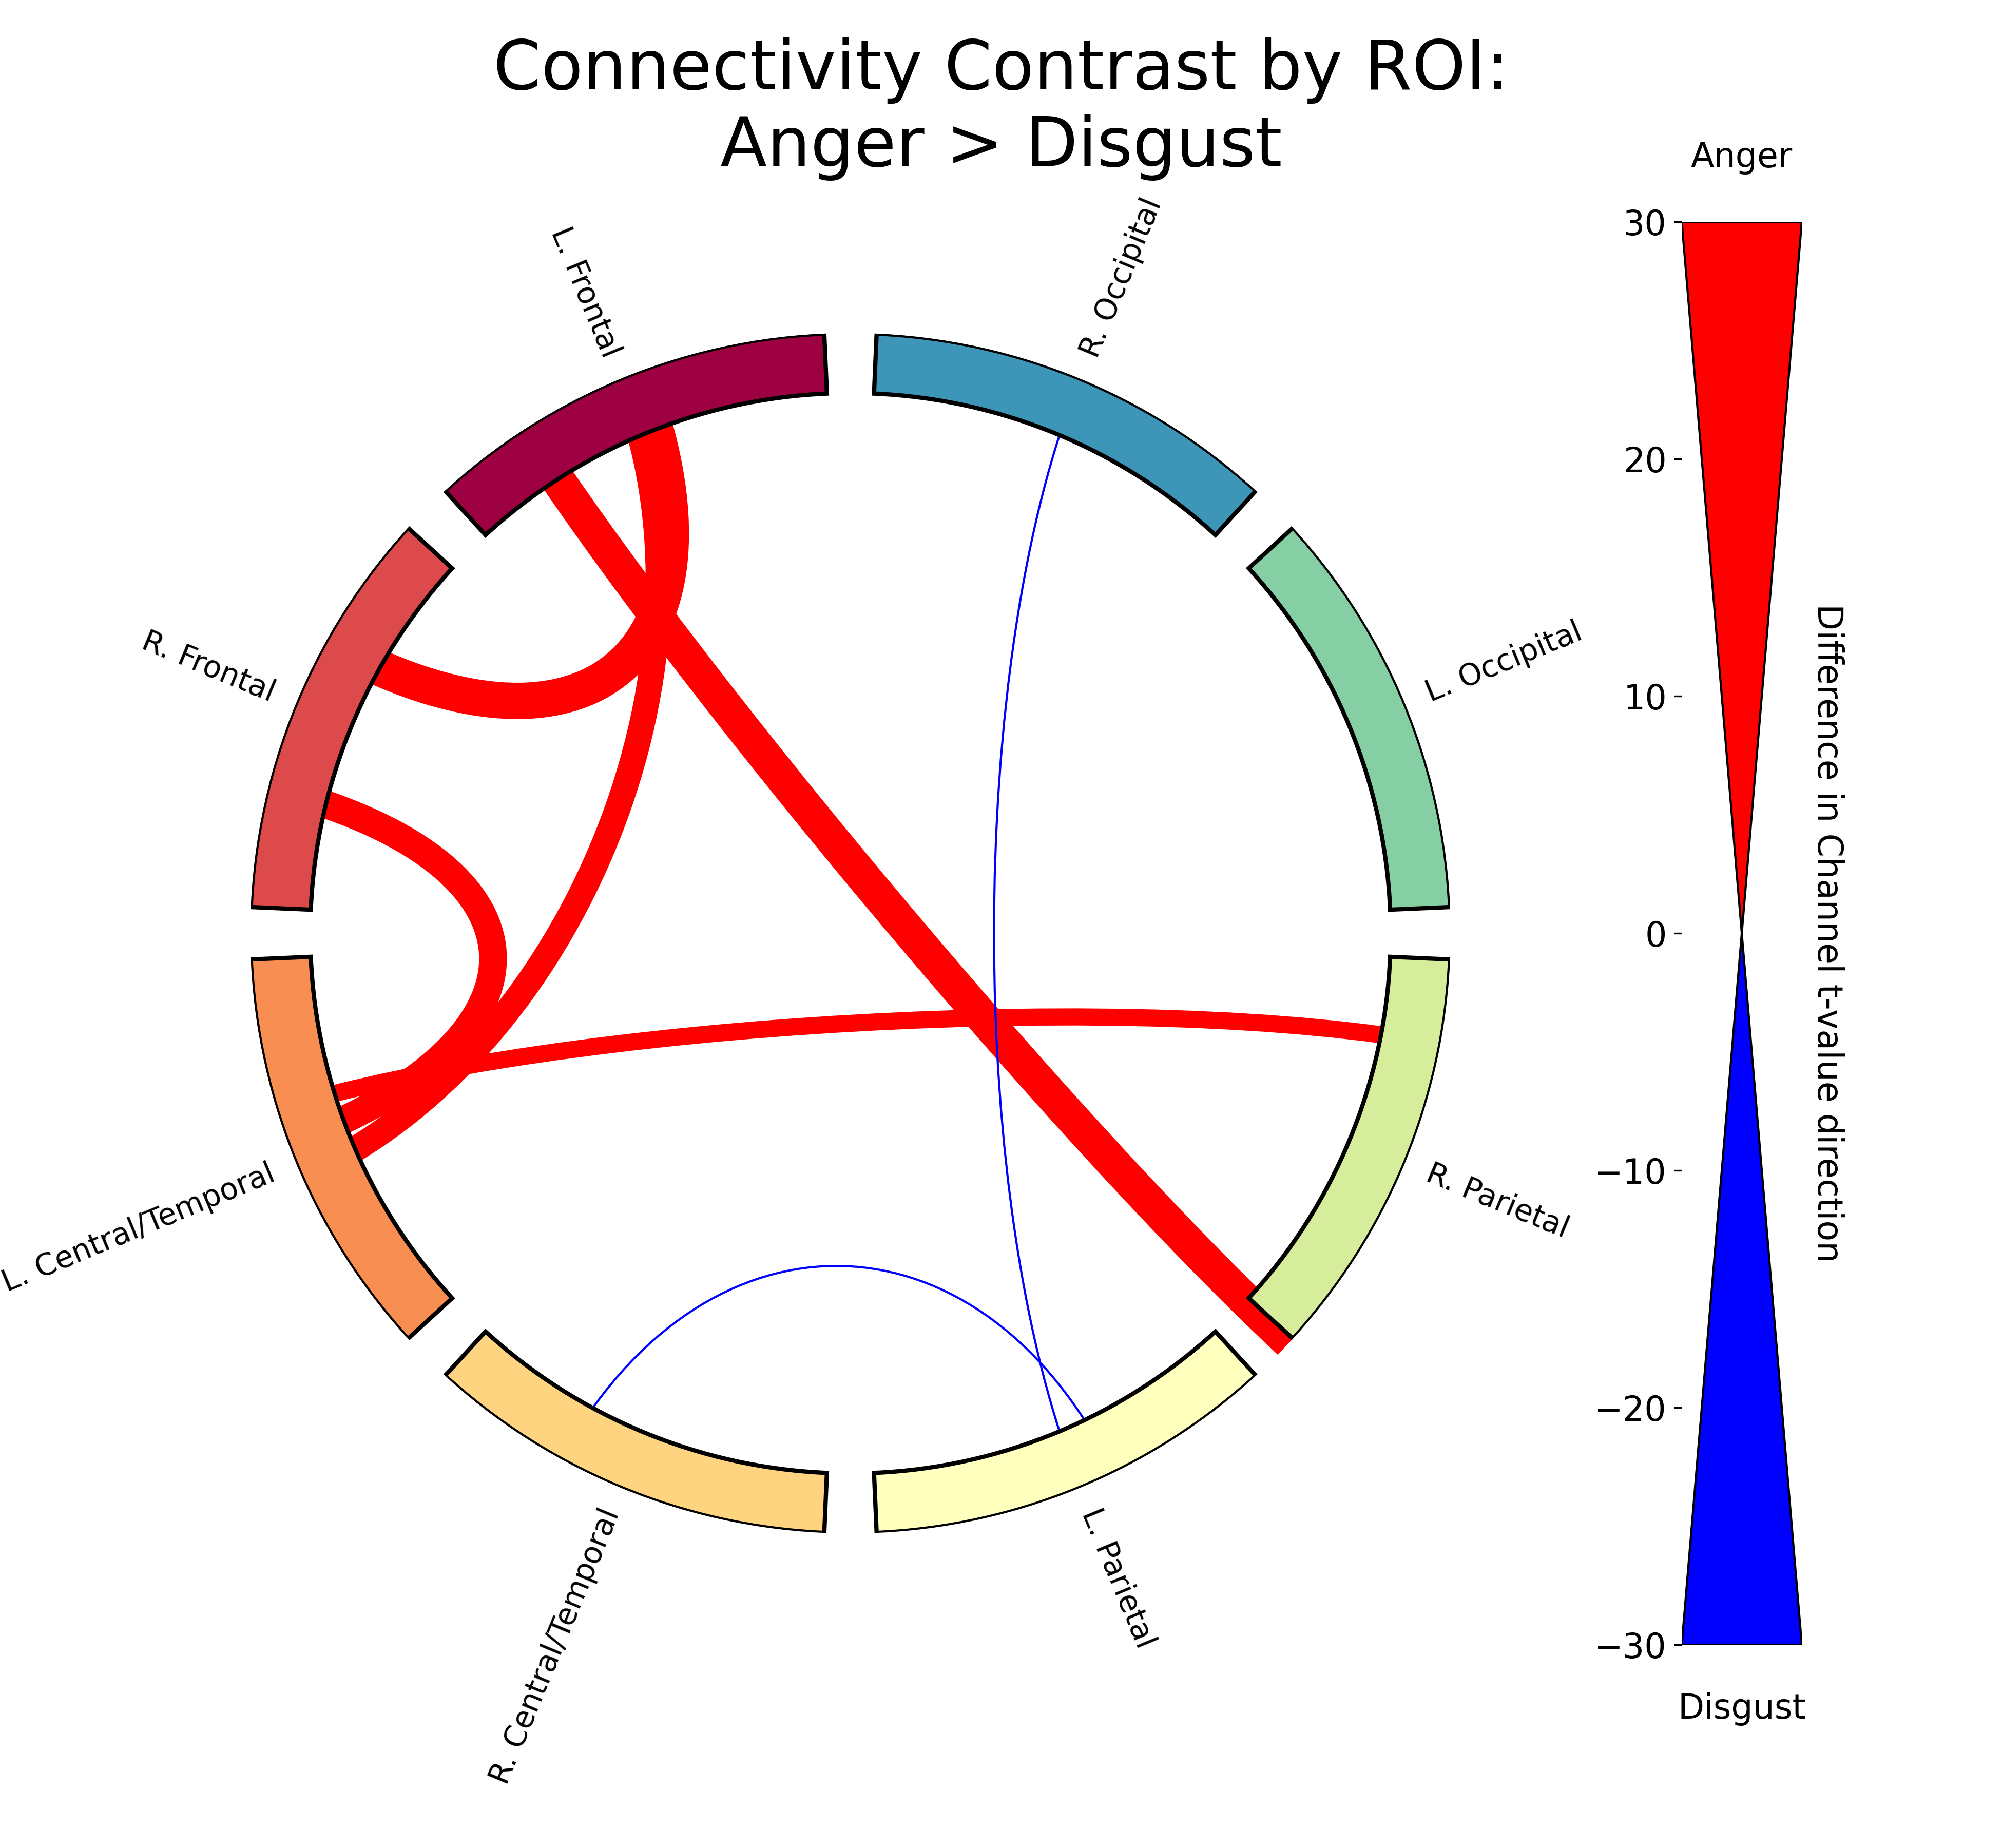
\includegraphics[width=0.45\textwidth]{C:/Users/super/OneDrive - Ontario Tech University/fNIRS_Emotions/plots/spectral_connectivity_time/chord_plots/group_level_t_tests_roi/emotion_Anger_Disgust.png}
    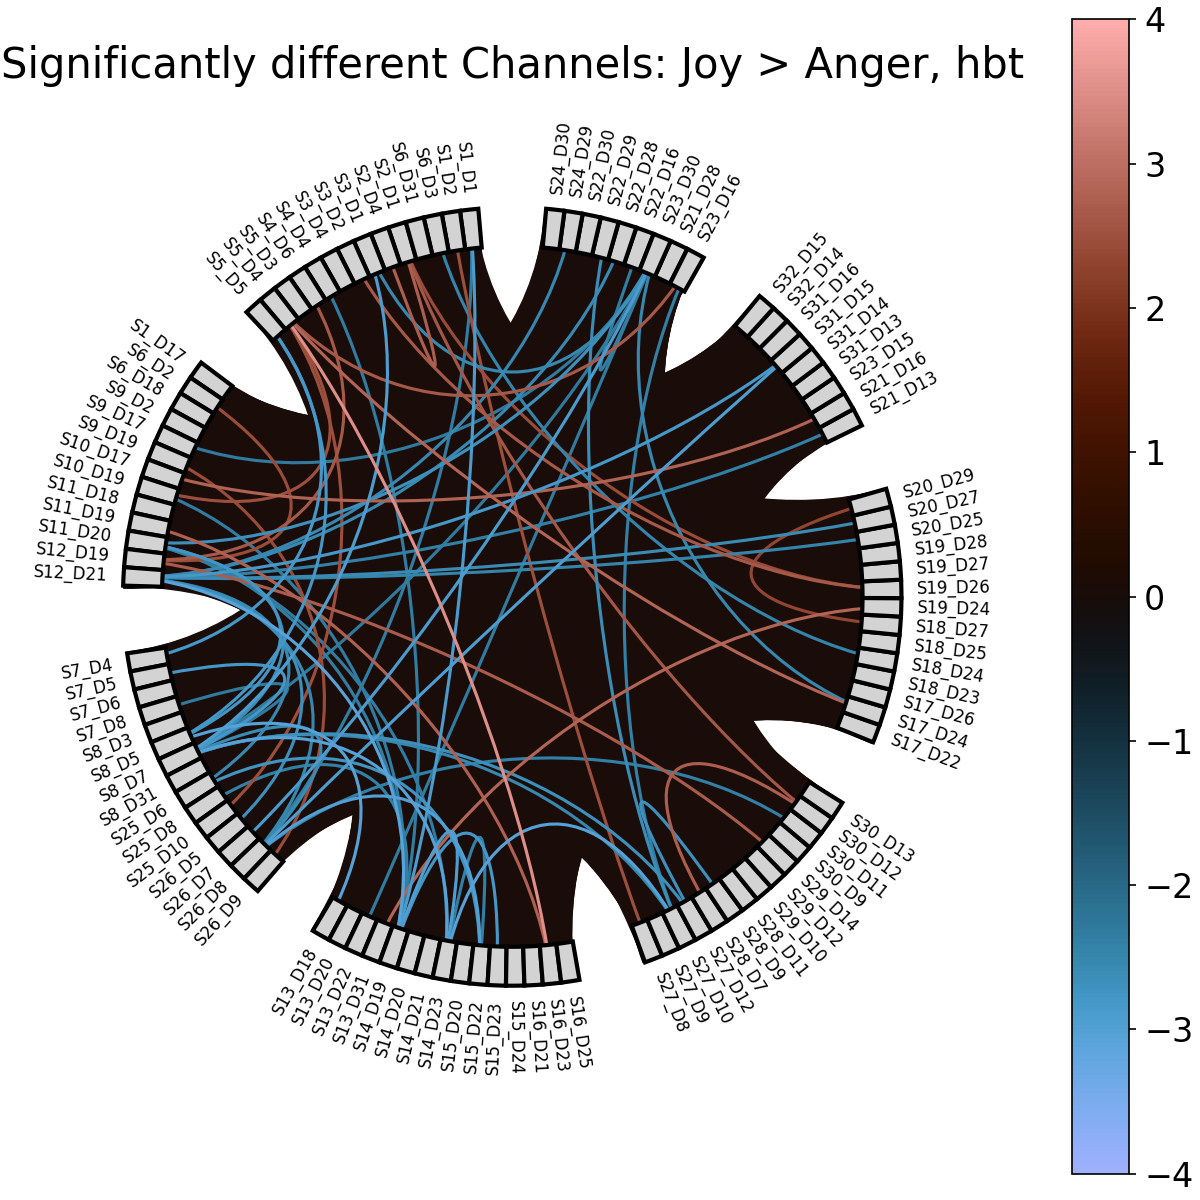
\includegraphics[width=0.45\textwidth]{C:/Users/super/OneDrive - Ontario Tech University/fNIRS_Emotions/plots/spectral_connectivity_time/chord_plots/group_level_t_tests_roi/emotion_Joy_Anger.png}
    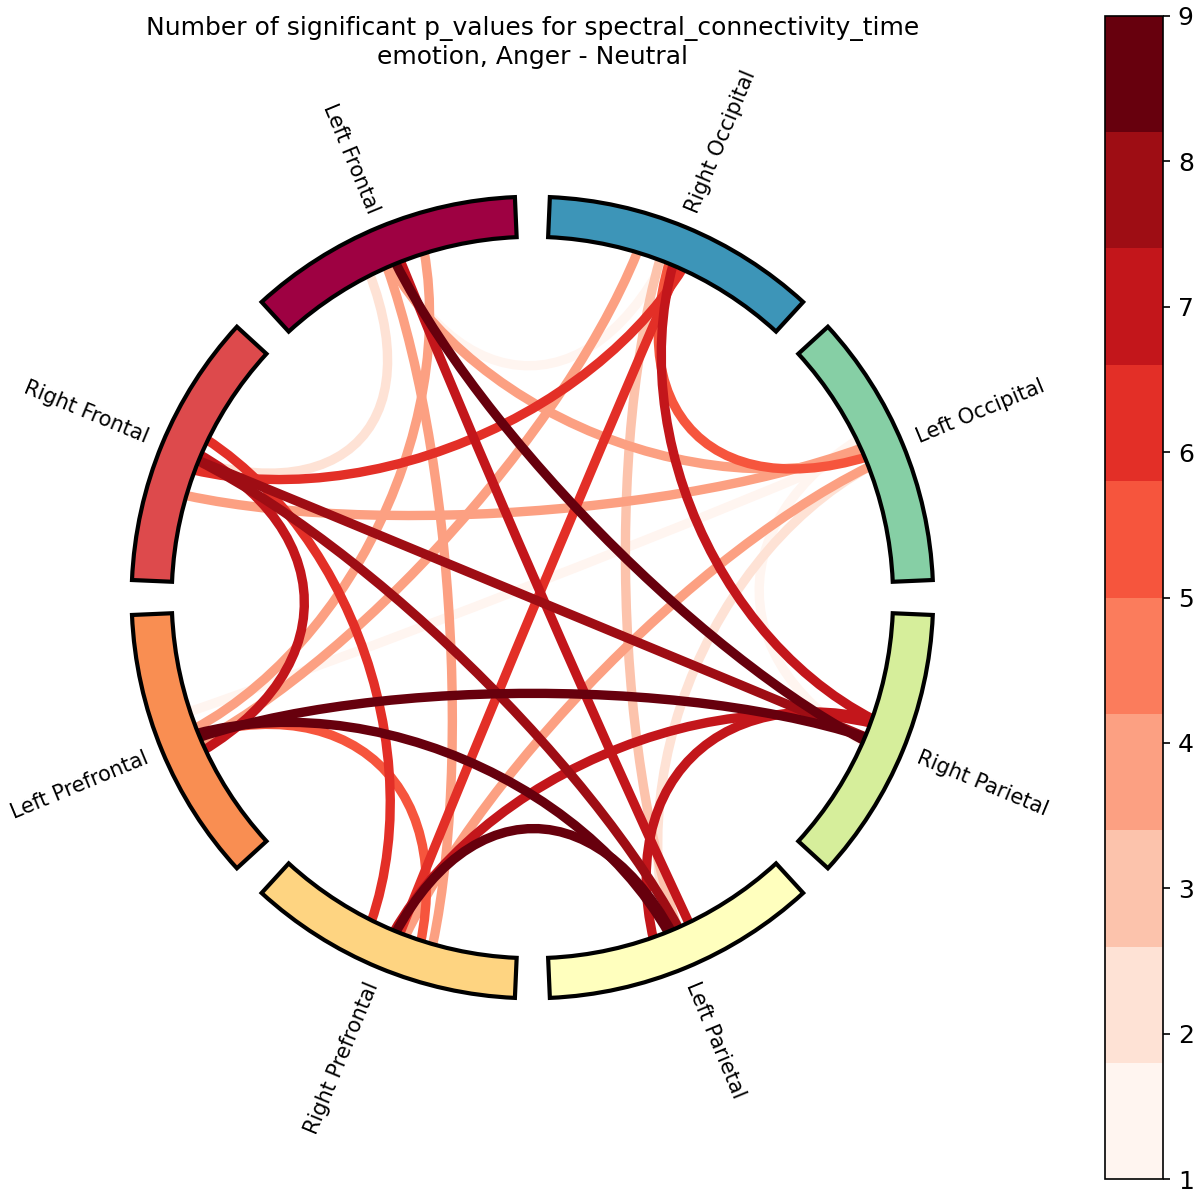
\includegraphics[width=0.45\textwidth]{C:/Users/super/OneDrive - Ontario Tech University/fNIRS_Emotions/plots/spectral_connectivity_time/chord_plots/group_level_t_tests_roi/emotion_Anger_Neutral.png}
    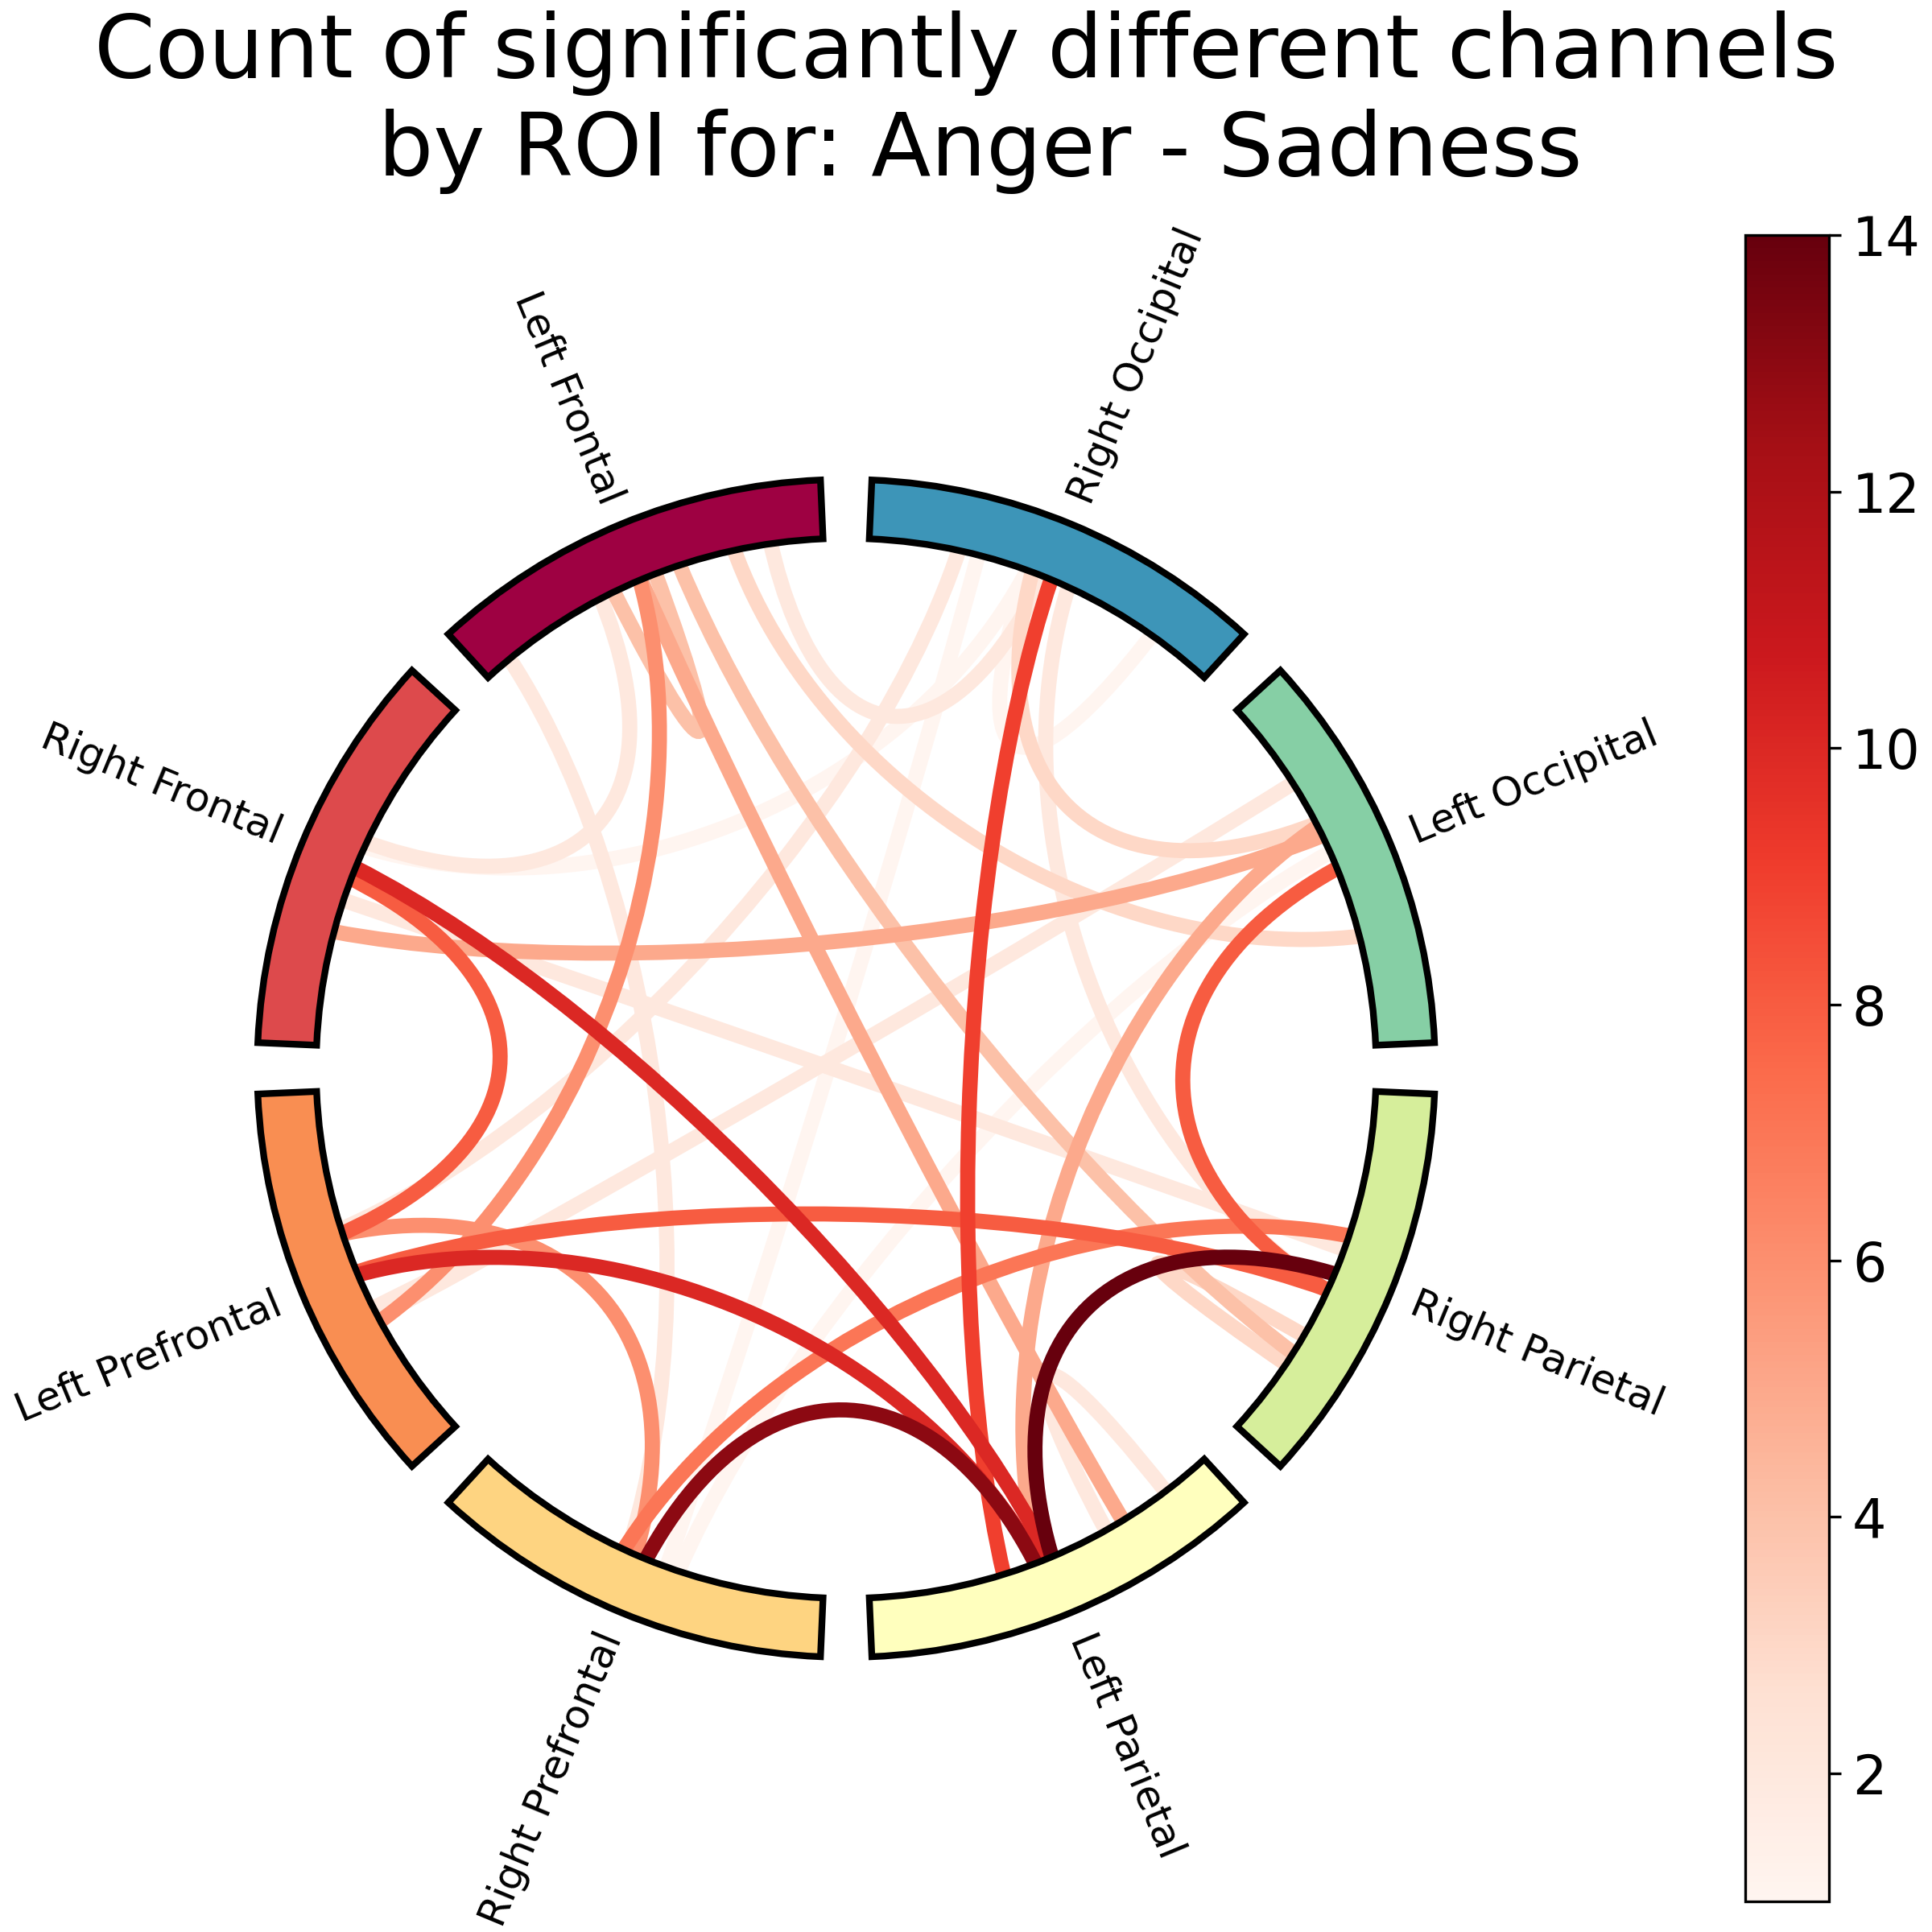
\includegraphics[width=0.45\textwidth]{C:/Users/super/OneDrive - Ontario Tech University/fNIRS_Emotions/plots/spectral_connectivity_time/chord_plots/group_level_t_tests_roi/emotion_Anger_Sadness.png}
    \caption[FC: Additional emotion contrasts]{Functional connectivity results for Anger contrasts: Anger vs. Disgust, Joy, Neutral, and Sadness. (1/4)}
    \label{fig:appendix_fc_emotion_analysis}
\end{figure}

\FloatBarrier

\begin{figure}[H]
    \ContinuedFloat
    \centering
    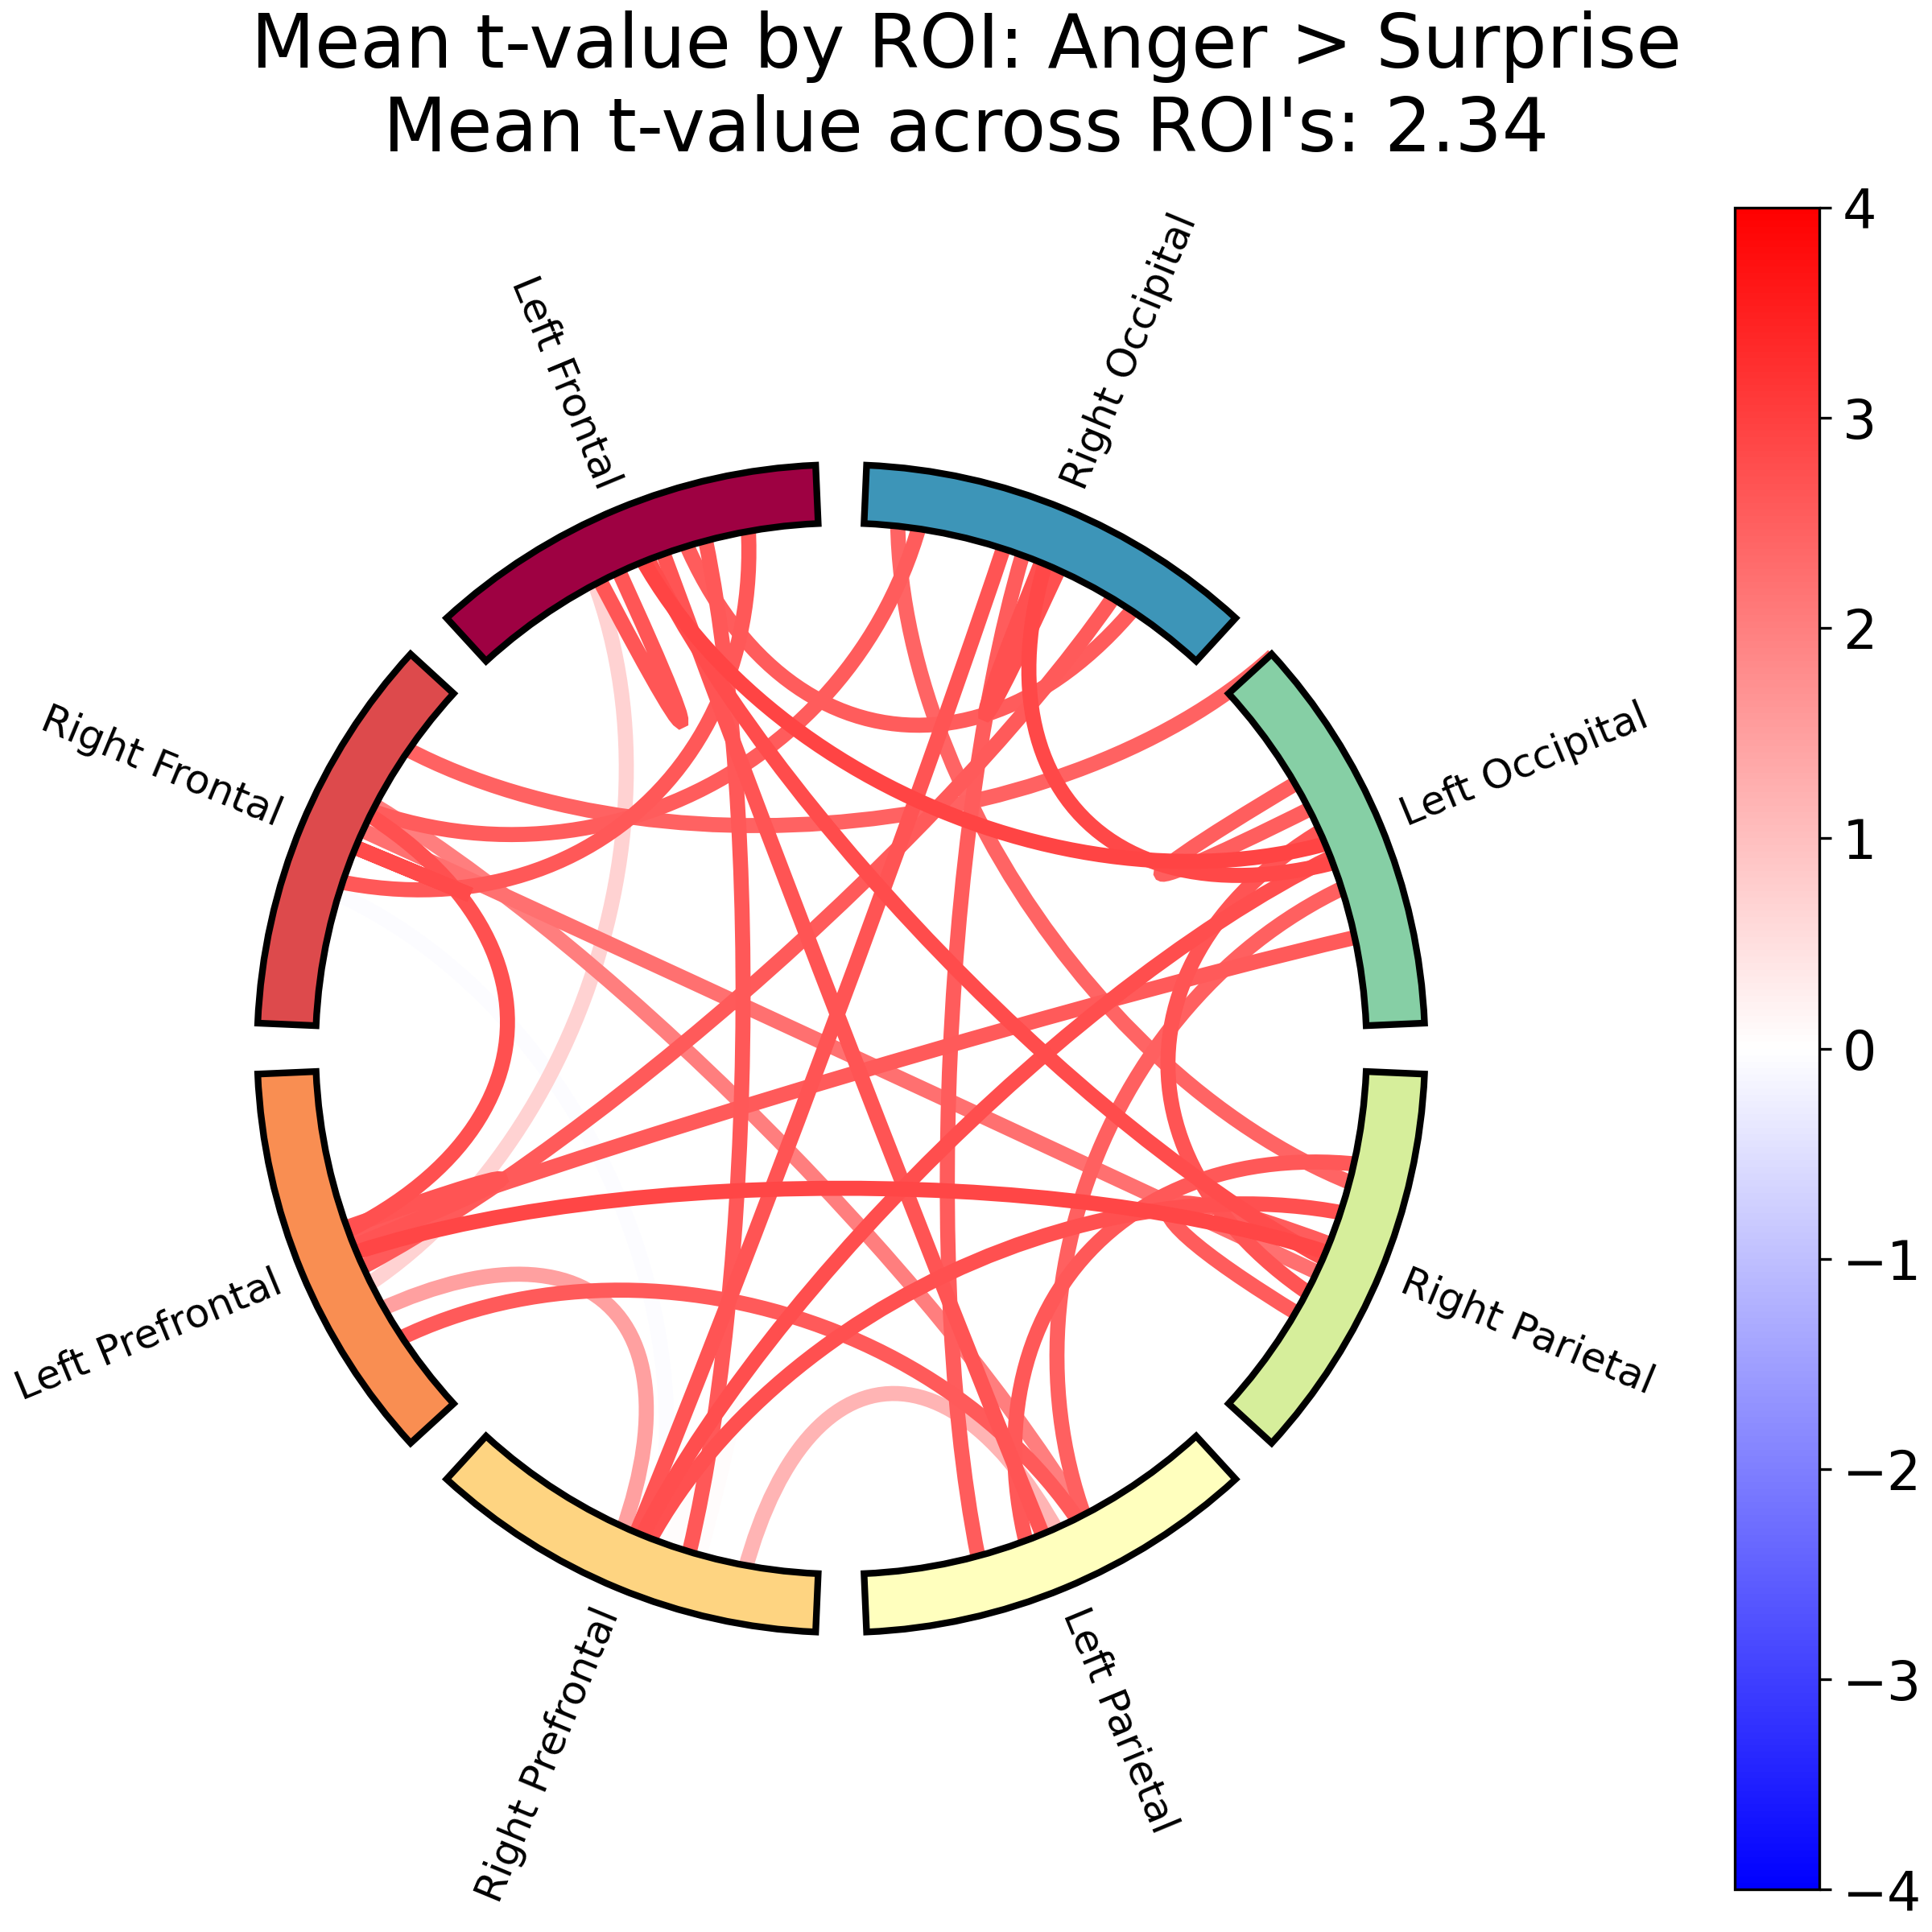
\includegraphics[width=0.49\textwidth]{C:/Users/super/OneDrive - Ontario Tech University/fNIRS_Emotions/plots/spectral_connectivity_time/chord_plots/group_level_t_tests_roi/emotion_Anger_Surprise.png}
    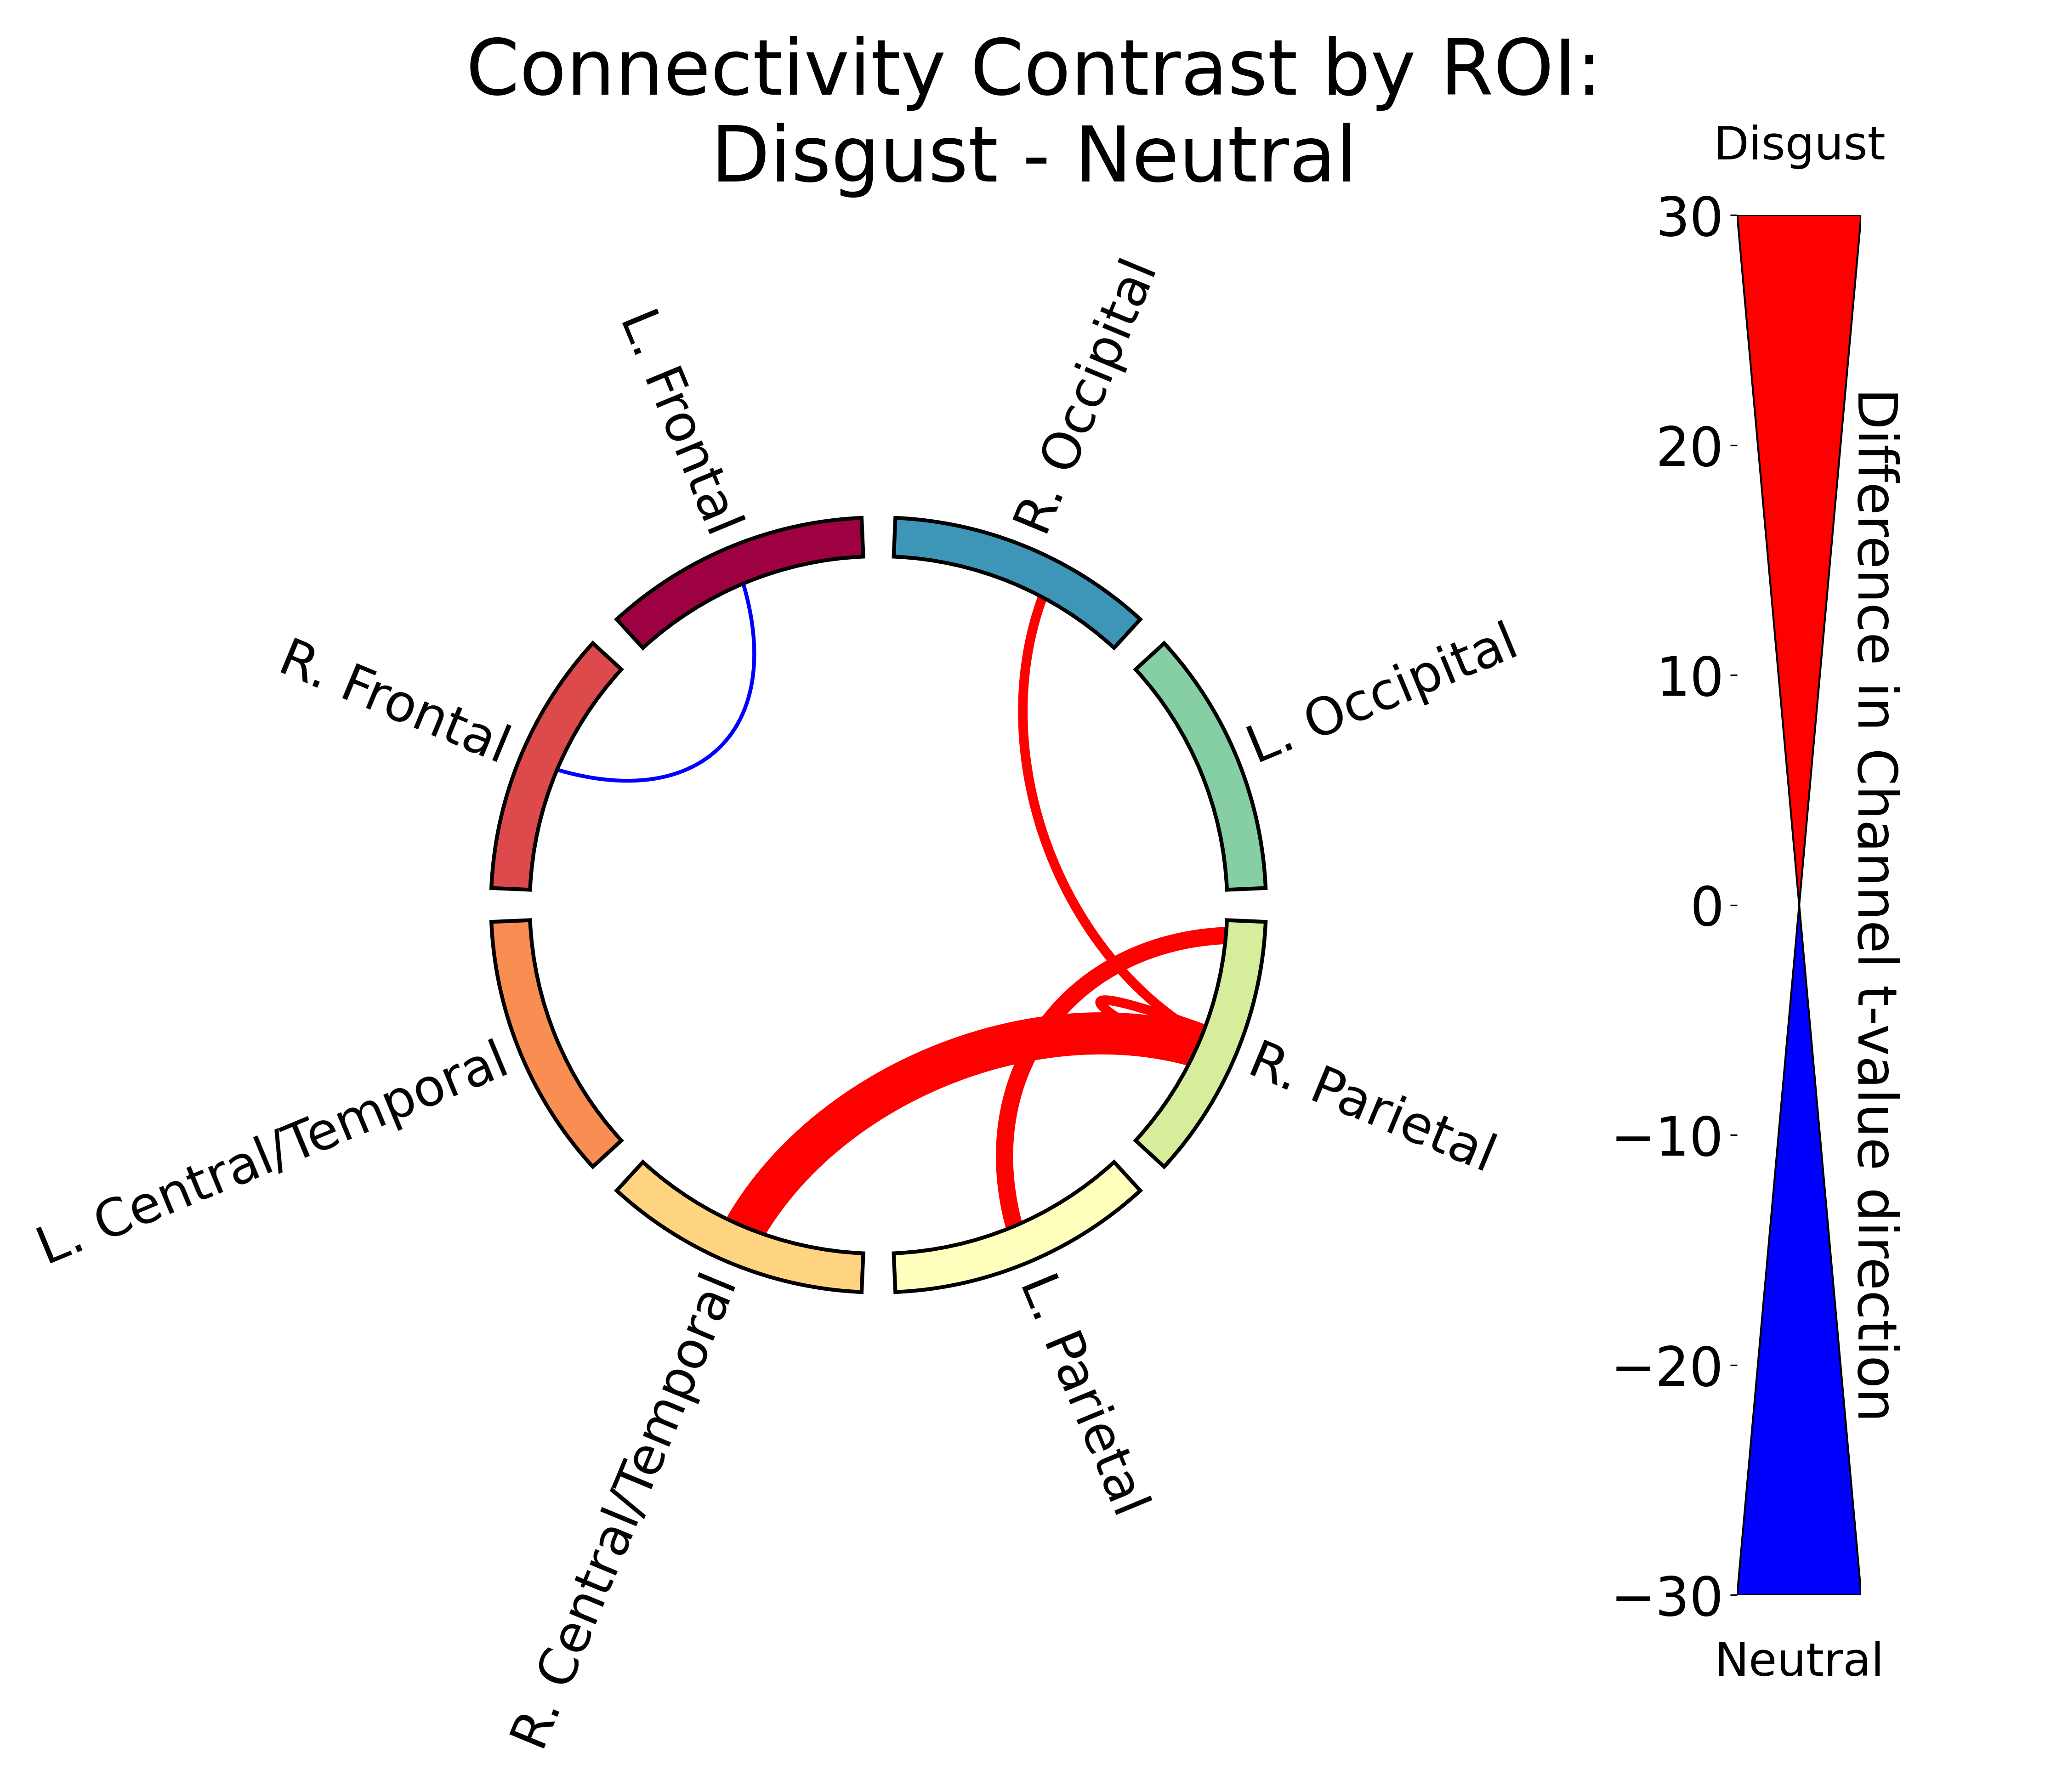
\includegraphics[width=0.49\textwidth]{C:/Users/super/OneDrive - Ontario Tech University/fNIRS_Emotions/plots/spectral_connectivity_time/chord_plots/group_level_t_tests_roi/emotion_Disgust_Neutral.png}
    \includegraphics[width=0.49\textwidth]{C:/Users/super/OneDrive - Ontario Tech University/fNIRS_Emotions/plots/spectral_connectivity_time/chord_plots/group_level_t_tests_roi/emotion_Disgust_Sadness.png}
    \includegraphics[width=0.49\textwidth]{C:/Users/super/OneDrive - Ontario Tech University/fNIRS_Emotions/plots/spectral_connectivity_time/chord_plots/group_level_t_tests_roi/emotion_Disgust_Surprise.png}
    \caption*{Functional connectivity results for Anger vs. Surprise and Disgust contrasts: Disgust vs. Neutral, Sadness, and Surprise. (2/4)}
\end{figure}

\FloatBarrier

\begin{figure}[H]
    \ContinuedFloat
    \centering
    \includegraphics[width=0.49\textwidth]{C:/Users/super/OneDrive - Ontario Tech University/fNIRS_Emotions/plots/spectral_connectivity_time/chord_plots/group_level_t_tests_roi/emotion_Joy_Disgust.png}
    \includegraphics[width=0.49\textwidth]{C:/Users/super/OneDrive - Ontario Tech University/fNIRS_Emotions/plots/spectral_connectivity_time/chord_plots/group_level_t_tests_roi/emotion_Joy_Neutral.png}
    \includegraphics[width=0.49\textwidth]{C:/Users/super/OneDrive - Ontario Tech University/fNIRS_Emotions/plots/spectral_connectivity_time/chord_plots/group_level_t_tests_roi/emotion_Joy_Sadness.png}
    \includegraphics[width=0.49\textwidth]{C:/Users/super/OneDrive - Ontario Tech University/fNIRS_Emotions/plots/spectral_connectivity_time/chord_plots/group_level_t_tests_roi/emotion_Joy_Surprise.png}
    \caption*{Functional connectivity results for Joy contrasts: Joy vs. Disgust, Neutral, Sadness, and Surprise. (3/4)}
\end{figure}

\FloatBarrier

\begin{figure}[H]
    \ContinuedFloat
    \centering
    \includegraphics[width=0.49\textwidth]{C:/Users/super/OneDrive - Ontario Tech University/fNIRS_Emotions/plots/spectral_connectivity_time/chord_plots/group_level_t_tests_roi/emotion_Neutral_Surprise.png}
    \includegraphics[width=0.49\textwidth]{C:/Users/super/OneDrive - Ontario Tech University/fNIRS_Emotions/plots/spectral_connectivity_time/chord_plots/group_level_t_tests_roi/emotion_Sadness_Neutral.png}
    \includegraphics[width=0.49\textwidth]{C:/Users/super/OneDrive - Ontario Tech University/fNIRS_Emotions/plots/spectral_connectivity_time/chord_plots/group_level_t_tests_roi/emotion_Sadness_Surprise.png}
    \caption*{Functional connectivity results for Neutral and Sadness contrasts: Neutral vs. Surprise, Sadness vs. Neutral, and Sadness vs. Surprise. (4/4)}
\end{figure}

\label{tab:appendix_fc_emotion_analysis}
\input{C:/Users/super/OneDrive - Ontario Tech University/fNIRS_Emotions/processed_data/spectral_connectivity_time/group_level_t_tests_roi_contrast_ratios.tex}

\chapter{Memory Task}
\section{ANOVA Results}
\label{tab:appendix_memory_task_anova}
\input{C:/Users/super/OneDrive - Ontario Tech University/fNIRS_Emotions/processed_data/behavioural_responses/anova_table.tex}

\section{Memory Task No Response Distribution}
\begin{figure}[H]
    \centering
    \includegraphics[width=1\textwidth]{C:/Users/super/OneDrive - Ontario Tech University/fNIRS_Emotions/plots/behavioural_responses/no_response_counts.png}
    \caption[Memory Task No Response Distribution]{Distribution of the number of no responses across the 56 blocks for each participant in the memory task.}
    \label{fig:appendix_memory_task_no_response_distribution}
\end{figure}

\end{document}

%%%%%%%%%%%%%%%%%%%%%%%%%%%%%%%%%%%%%%%%%%%%%%%%%%%%%%%%%%%%%%%%%%%%%%
%%  End of ONTARIOTECHU-THESIS.TEX
%%%%%%%%%%%%%%%%%%%%%%%%%%%%%%%%%%%%%%%%%%%%%%%%%%%%%%%%%%%%%%%%%%%%%%
